\documentclass{article}

\usepackage{forest}
\usetikzlibrary[intersections]
\usetikzlibrary[decorations.pathreplacing]
\usepackage{html}
\usepackage{graphicx}
\usepackage{tikz}

\usetikzlibrary[arrows.meta,backgrounds,calc,fit,positioning,shapes.multipart]

% Also ****ing broken.
%\newenvironment{ezcode}{\begin{quote}\begin{verbatim}}{\end{verbatim}\end{quote}}

\begin{document}

This page contains links to writings about topics such as technology, video games, and philosophy.

\tableofchildlinks*

% Recompiling the Novena Linux Kernel Woes
\section{2019-05-07 Recompiling the Novena Linux Kernel Woes}
Normally when I have kernel problems they happen during a kernel upgrade, but not this time.  In fact, I'm not even sure \emph{when} the issues started happening.  Everything seemed fine at first, until one day when I tried to mount a USB storage device only to find that it wasn't working; instead, I got an error along the following lines (except not the \texttt{ipv6} module, obviously):

\begin{quote}
\begin{verbatim}
	[  622.972948] ipv6: no symbol version for module_layout
\end{verbatim}
\end{quote}

What could have caused this?  I'd done several major system upgrades since last time I recall modules working, but more suspect was the \texttt{CHOST} \htmladdnormallink{change}{https://www.gentoo.org/support/news-items/2018-09-07-arm-17-profile-migration.html}.  Well, it wasn't (and still isn't) clear to me exactly how much the \texttt{CHOST} change might affect the kernel, so the simplest solution would be to simply recompile the kernel, right?  That's when this happened:

\begin{quote}
\begin{verbatim}
	  CC      kernel/fork.o
	In file included from include/linux/kernel.h:11,
	                 from include/asm-generic/bug.h:13,
	                 from ./arch/arm/include/asm/bug.h:59,
	                 from include/linux/bug.h:4,
	                 from include/linux/mmdebug.h:4,
	                 from include/linux/gfp.h:4,
	                 from include/linux/slab.h:14,
	                 from kernel/fork.c:14:
	include/linux/log2.h:22:1: warning: ignoring attribute 'noreturn' because it  \
	conflicts with attribute 'const' [-Wattributes]
	 int ____ilog2_NaN(void);
	 ^~~
	In file included from kernel/fork.c:41:
	include/linux/syscalls.h:195:18: warning: 'sys_set_tid_address' alias between \
	functions of incompatible types 'long int(int *)' and 'long int(long int)'    \
	[-Wattribute-alias]
	  asmlinkage long sys##name(__MAP(x,__SC_DECL,__VA_ARGS__)) \
	                  ^~~
	include/linux/syscalls.h:191:2: note: in expansion of macro '__SYSCALL_DEFINEx'
	  __SYSCALL_DEFINEx(x, sname, __VA_ARGS__)
	  ^~~~~~~~~~~~~~~~~
	include/linux/syscalls.h:182:36: note: in expansion of macro 'SYSCALL_DEFINEx'
	 #define SYSCALL_DEFINE1(name, ...) SYSCALL_DEFINEx(1, _##name, __VA_ARGS__)
	                                    ^~~~~~~~~~~~~~~
	kernel/fork.c:1236:1: note: in expansion of macro 'SYSCALL_DEFINE1'
	 SYSCALL_DEFINE1(set_tid_address, int __user *, tidptr)
	 ^~~~~~~~~~~~~~~
	include/linux/syscalls.h:199:18: note: aliased declaration here
	  asmlinkage long SyS##name(__MAP(x,__SC_LONG,__VA_ARGS__)) \
	                  ^~~
	include/linux/syscalls.h:191:2: note: in expansion of macro '__SYSCALL_DEFINEx'
	  __SYSCALL_DEFINEx(x, sname, __VA_ARGS__)
	  ^~~~~~~~~~~~~~~~~
	include/linux/syscalls.h:182:36: note: in expansion of macro 'SYSCALL_DEFINEx'
	 #define SYSCALL_DEFINE1(name, ...) SYSCALL_DEFINEx(1, _##name, __VA_ARGS__)
	                                    ^~~~~~~~~~~~~~~
	kernel/fork.c:1236:1: note: in expansion of macro 'SYSCALL_DEFINE1'
	 SYSCALL_DEFINE1(set_tid_address, int __user *, tidptr)
	 ^~~~~~~~~~~~~~~
	include/linux/syscalls.h:195:18: warning: 'sys_unshare' alias between functions \
	of incompatible types 'long int(long unsigned int)' and 'long int(long int)' \
	[-Wattribute-alias]
	  asmlinkage long sys##name(__MAP(x,__SC_DECL,__VA_ARGS__)) \
	                  ^~~
	include/linux/syscalls.h:191:2: note: in expansion of macro '__SYSCALL_DEFINEx'
	  __SYSCALL_DEFINEx(x, sname, __VA_ARGS__)
	  ^~~~~~~~~~~~~~~~~
	include/linux/syscalls.h:182:36: note: in expansion of macro 'SYSCALL_DEFINEx'
	 #define SYSCALL_DEFINE1(name, ...) SYSCALL_DEFINEx(1, _##name, __VA_ARGS__)
	                                    ^~~~~~~~~~~~~~~
	kernel/fork.c:2000:1: note: in expansion of macro 'SYSCALL_DEFINE1'
	 SYSCALL_DEFINE1(unshare, unsigned long, unshare_flags)
	 ^~~~~~~~~~~~~~~
	include/linux/syscalls.h:199:18: note: aliased declaration here
	  asmlinkage long SyS##name(__MAP(x,__SC_LONG,__VA_ARGS__)) \
	                  ^~~
	include/linux/syscalls.h:191:2: note: in expansion of macro '__SYSCALL_DEFINEx'
	  __SYSCALL_DEFINEx(x, sname, __VA_ARGS__)
	  ^~~~~~~~~~~~~~~~~
	include/linux/syscalls.h:182:36: note: in expansion of macro 'SYSCALL_DEFINEx'
	 #define SYSCALL_DEFINE1(name, ...) SYSCALL_DEFINEx(1, _##name, __VA_ARGS__)
	                                    ^~~~~~~~~~~~~~~
	kernel/fork.c:2000:1: note: in expansion of macro 'SYSCALL_DEFINE1'
	 SYSCALL_DEFINE1(unshare, unsigned long, unshare_flags)
	 ^~~~~~~~~~~~~~~
	include/linux/syscalls.h:195:18: warning: 'sys_clone' alias between functions \
	of incompatible types 'long int(long unsigned int,  long unsigned int,  int *, \
	long unsigned int,  int *)' and 'long int(long int,  long int,  long int,  \
	long int,  long int)' [-Wattribute-alias]
	  asmlinkage long sys##name(__MAP(x,__SC_DECL,__VA_ARGS__)) \
	                  ^~~
	include/linux/syscalls.h:191:2: note: in expansion of macro '__SYSCALL_DEFINEx'
	  __SYSCALL_DEFINEx(x, sname, __VA_ARGS__)
	  ^~~~~~~~~~~~~~~~~
	include/linux/syscalls.h:186:36: note: in expansion of macro 'SYSCALL_DEFINEx'
	 #define SYSCALL_DEFINE5(name, ...) SYSCALL_DEFINEx(5, _##name, __VA_ARGS__)
	                                    ^~~~~~~~~~~~~~~
	kernel/fork.c:1849:1: note: in expansion of macro 'SYSCALL_DEFINE5'
	 SYSCALL_DEFINE5(clone, unsigned long, clone_flags, unsigned long, newsp,
	 ^~~~~~~~~~~~~~~
	include/linux/syscalls.h:199:18: note: aliased declaration here
	  asmlinkage long SyS##name(__MAP(x,__SC_LONG,__VA_ARGS__)) \
	                  ^~~
	include/linux/syscalls.h:191:2: note: in expansion of macro '__SYSCALL_DEFINEx'
	  __SYSCALL_DEFINEx(x, sname, __VA_ARGS__)
	  ^~~~~~~~~~~~~~~~~
	include/linux/syscalls.h:186:36: note: in expansion of macro 'SYSCALL_DEFINEx'
	 #define SYSCALL_DEFINE5(name, ...) SYSCALL_DEFINEx(5, _##name, __VA_ARGS__)
	                                    ^~~~~~~~~~~~~~~
	kernel/fork.c:1849:1: note: in expansion of macro 'SYSCALL_DEFINE5'
	 SYSCALL_DEFINE5(clone, unsigned long, clone_flags, unsigned long, newsp,
	 ^~~~~~~~~~~~~~~
	/tmp/ccxt2fNN.s: Assembler messages:
	/tmp/ccxt2fNN.s:5608: Error: .err encountered
	make[1]: *** [scripts/Makefile.build:290: kernel/fork.o] Error 1
	make: *** [Makefile:987: kernel] Error 2
\end{verbatim}
\end{quote}

"Oh, a system call error, this will be an easy fix", said no one, ever.  At this point I decided to run away screaming from the problem, but, after many months, I eventually got tired of not being able to use modules (or compile them into the kernel) and decided to buckle down and fix the problem.  As I suspected, it took a lot of guesswork.

\subsection{Troubleshooting}

I decided to begin by looking for low-hanging fruit.  Perhaps some simple configuration options, or a forgotten PEBKAC.  One hopeful candidate was to enable the \texttt{CONFIG_OABI_COMPAT} option, but it didn't help.  The next was to save the \texttt{.config} file, then re-emerge the kernel sources, you know, in case it had become\ldots~corrupted.  Or something.  That also failed to solve the problem.  The easy stuff was out, so it was time to look at the source.  The system call definitions in the file \texttt{include/linux/syscalls.h} showed:

\begin{quote}
\begin{verbatim}
	#define SYSCALL_DEFINE1(name, ...) SYSCALL_DEFINEx(1, _##name, __VA_ARGS__)
	#define SYSCALL_DEFINE2(name, ...) SYSCALL_DEFINEx(2, _##name, __VA_ARGS__)
	#define SYSCALL_DEFINE3(name, ...) SYSCALL_DEFINEx(3, _##name, __VA_ARGS__)
	#define SYSCALL_DEFINE4(name, ...) SYSCALL_DEFINEx(4, _##name, __VA_ARGS__)
	#define SYSCALL_DEFINE5(name, ...) SYSCALL_DEFINEx(5, _##name, __VA_ARGS__)
	#define SYSCALL_DEFINE6(name, ...) SYSCALL_DEFINEx(6, _##name, __VA_ARGS__)

	#define SYSCALL_DEFINEx(x, sname, ...)				\
		SYSCALL_METADATA(sname, x, __VA_ARGS__)			\
		__SYSCALL_DEFINEx(x, sname, __VA_ARGS__)

	#define __PROTECT(...) asmlinkage_protect(__VA_ARGS__)
	#define __SYSCALL_DEFINEx(x, name, ...)					\
		asmlinkage long sys##name(__MAP(x,__SC_DECL,__VA_ARGS__))	\
			__attribute__((alias(__stringify(SyS##name))));		\
		static inline long SYSC##name(__MAP(x,__SC_DECL,__VA_ARGS__));	\
		asmlinkage long SyS##name(__MAP(x,__SC_LONG,__VA_ARGS__));	\
		asmlinkage long SyS##name(__MAP(x,__SC_LONG,__VA_ARGS__))	\
		{								\
			long ret = SYSC##name(__MAP(x,__SC_CAST,__VA_ARGS__));	\
			__MAP(x,__SC_TEST,__VA_ARGS__);				\
			__PROTECT(x, ret,__MAP(x,__SC_ARGS,__VA_ARGS__));	\
			return ret;						\
		}								\
		static inline long SYSC##name(__MAP(x,__SC_DECL,__VA_ARGS__))
\end{verbatim}
\end{quote}

\ldots and the clone system call definition in \texttt{kernel/fork.c} was:

\begin{quote}
\begin{verbatim}
#ifdef __ARCH_WANT_SYS_CLONE
#ifdef CONFIG_CLONE_BACKWARDS
SYSCALL_DEFINE5(clone, unsigned long, clone_flags, unsigned long, newsp,
		 int __user *, parent_tidptr,
		 unsigned long, tls,
		 int __user *, child_tidptr)
#elif defined(CONFIG_CLONE_BACKWARDS2)
SYSCALL_DEFINE5(clone, unsigned long, newsp, unsigned long, clone_flags,
		 int __user *, parent_tidptr,
		 int __user *, child_tidptr,
		 unsigned long, tls)
#elif defined(CONFIG_CLONE_BACKWARDS3)
SYSCALL_DEFINE6(clone, unsigned long, clone_flags, unsigned long, newsp,
		int, stack_size,
		int __user *, parent_tidptr,
		int __user *, child_tidptr,
		unsigned long, tls)
#else
SYSCALL_DEFINE5(clone, unsigned long, clone_flags, unsigned long, newsp,
		 int __user *, parent_tidptr,
		 int __user *, child_tidptr,
		 unsigned long, tls)
#endif
{
	return _do_fork(clone_flags, newsp, 0, parent_tidptr, child_tidptr, tls);
}
#endif
\end{verbatim}
\end{quote}

I spent a good amount of time staring at this code, and still didn't truly understand it.  The macros existed in order to define system calls, with the various numbers corresponding to the number of arguments passed to the system call.  The other stuff?  Dragons.  Looking at the "backwards" cloning showed that it wasn't really a toggleable option, though an amusing comment was left in \texttt{arch/Kconfig}: "\texttt{# ABI hall of shame}".  I couldn't glean any clues from staring at the code, so I decided to switch gears towards the \htmladdnormallink{Novena patchset}{https://github.com/clinew/novena-kernel-patches/releases/tag/v4.7.2-r1} in order to see if any of those patches may have tweaked the system call code.  They didn't, and I couldn't find any clues.  Perhaps, because the kernel was old, the \texttt{CHOST} change had not taken effect in the kernel and was mismatched with the system?  A \texttt{grep} through the source code showed the opposite; the kernel had changed way before my user space had!  An Internet search returned this \htmladdnormallink{mail thread}{https://lkml.org/lkml/2018/6/30/143} which showed a similar error, but \texttt{KCOV} wasn't enabled in my kernel, so it was also a dead end.

Stumped, I decided that, surely, someone else must have run into the issue and had probably already fixed the issue in a later kernel.  Looking at the latest source, \texttt{v5.1-rc6} at the time, showed that the system calls had changed to:

\begin{quote}
\begin{verbatim}
	/*
	 * The asmlinkage stub is aliased to a function named __se_sys_*() which
	 * sign-extends 32-bit ints to longs whenever needed. The actual work is
	 * done within __do_sys_*().
	 */
	#ifndef __SYSCALL_DEFINEx
	#define __SYSCALL_DEFINEx(x, name, ...)					\
		__diag_push();							\
		__diag_ignore(GCC, 8, "-Wattribute-alias",			\
			      "Type aliasing is used to sanitize syscall arguments");\
		asmlinkage long sys##name(__MAP(x,__SC_DECL,__VA_ARGS__))	\
			__attribute__((alias(__stringify(__se_sys##name))));	\
		ALLOW_ERROR_INJECTION(sys##name, ERRNO);			\
		static inline long __do_sys##name(__MAP(x,__SC_DECL,__VA_ARGS__));\
		asmlinkage long __se_sys##name(__MAP(x,__SC_LONG,__VA_ARGS__));	\
		asmlinkage long __se_sys##name(__MAP(x,__SC_LONG,__VA_ARGS__))	\
		{								\
			long ret = __do_sys##name(__MAP(x,__SC_CAST,__VA_ARGS__));\
			__MAP(x,__SC_TEST,__VA_ARGS__);				\
			__PROTECT(x, ret,__MAP(x,__SC_ARGS,__VA_ARGS__));	\
			return ret;						\
		}								\
		__diag_pop();							\
		static inline long __do_sys##name(__MAP(x,__SC_DECL,__VA_ARGS__))
	#endif /* __SYSCALL_DEFINEx */
\end{verbatim}
\end{quote}

This is a fair bit of churn, but it could be divided into at least 3 changes: 1) the \texttt{__diag} functions, 2) the \texttt{__se_sys} and \texttt{__do_sys} macros, and the 3) \texttt{ALLOW_ERROR_INJECTION} changes.  Using \texttt{git blame} to track the relevant commits down, I found out from commit \texttt{bee20031772af3debe8cbaa234528f24c7892e8f} that the \texttt{__diag*} functions existed in order to suppress the warnings that I was seeing; helpful, but this still left me with the compilation error.  The \texttt{__se_sys*} and \texttt{__do_sys*} macro changes were simply cleanups of the syscall stubs, as documented in commit \texttt{e145242ea0df6b7d28fd7186e61d6840fa4bb06e}.  Though none of the changes so far looked like they'd break the compilation, I nonetheless tried porting the patches and re-compiling; I succeeded in porting and suppressing the warning, but still had the compilation failure.  I never looked into \texttt{ALLOW_ERROR_INJECTION} as it didn't seem relevant.

Foiled once again, I decided to see if I could get the assembly code generated during compilation, as the temporary files were being cleaned up automatically after the error.  First I needed to find the build command.  It turned out that running \texttt{make V=1} increased the verbosity of the kernel compilation process enough that I could then view the commands being issued.  This is what I got:

\begin{quote}
\begin{verbatim}
	gcc -Wp,-MD,kernel/.fork.o.d  -nostdinc -isystem \
	/usr/lib/gcc/armv7a-unknown-linux-gnueabihf/8.2.0/include \
	-I./arch/arm/include -Iarch/arm/include/generated/uapi \
	-Iarch/arm/include/generated  -Iinclude -I./arch/arm/include/uapi \
	-Iarch/arm/include/generated/uapi -I./include/uapi \
	-Iinclude/generated/uapi -include ./include/linux/kconfig.h -D__KERNEL__ \
	-mlittle-endian -Wall -Wundef -Wstrict-prototypes -Wno-trigraphs \
	-fno-strict-aliasing -fno-common -Werror-implicit-function-declaration \
	-Wno-format-security -std=gnu89 -fno-dwarf2-cfi-asm -fno-omit-frame-pointer \
	-mapcs -mno-sched-prolog -fno-ipa-sra -mabi=aapcs-linux -mno-thumb-interwork \
	-mfpu=vfp -marm -D__LINUX_ARM_ARCH__=7 -march=armv7-a -msoft-float -Uarm \
	-fno-delete-null-pointer-checks -O2 --param=allow-store-data-races=0 \
	-fno-reorder-blocks -fno-ipa-cp-clone -fno-partial-inlining \
	-Wframe-larger-than=1024 -fno-stack-protector -Wno-unused-but-set-variable \
	-Wno-unused-const-variable -fno-omit-frame-pointer \
	-fno-optimize-sibling-calls -fno-var-tracking-assignments -g -gdwarf-4 -pg \
	-Wdeclaration-after-statement -Wno-pointer-sign -fno-strict-overflow \
	-fconserve-stack -Werror=implicit-int -Werror=strict-prototypes \
	-Werror=date-time -Werror=incompatible-pointer-types    \
	-DKBUILD_BASENAME='"fork"'  -DKBUILD_MODNAME='"fork"' -c -o \
	kernel/.tmp_fork.o kernel/fork.c
\end{verbatim}
\end{quote}

Luckily for me, simply running this command alone would reproduce the issue, but I still needed to have it preserve the assembly code.  After asking in \texttt{#kosagi} on the OFTC IRC channel I was told by \texttt{Jookia} that I could use either \texttt{-E} or \texttt{-S} to get the generated code.  Using \texttt{-E} generated the preprocessor output while \texttt{-S} generated the assembler output; I saved both.  Jumping to the line in the assembly code which caused the failure I saw:

\begin{quote}
\begin{verbatim}
	.LVL229:
		.loc 1 931 4 is_stmt 0 view .LVU1551
		.syntax divided
	@ 931 "kernel/fork.c" 1
		.ifnc r0,r0; .ifnc r0r0,fpr11; .ifnc r0r0,r11fp; .ifnc r0r0,ipr12; \
		.ifnc r0r0,r12ip; .err; .endif; .endif; .endif; .endif; .endif
		.ifnc r3,r2; .ifnc r3r2,fpr11; .ifnc r3r2,r11fp; .ifnc r3r2,ipr12; \
		.ifnc r3r2,r12ip; .err; .endif; .endif; .endif; .endif; .endif
		.ifnc r1,r1; .ifnc r1r1,fpr11; .ifnc r1r1,r11fp; .ifnc r1r1,ipr12; \
		.ifnc r1r1,r12ip; .err; .endif; .endif; .endif; .endif; .endif
		bl	__put_user_4
	@ 0 "" 2
\end{verbatim}
\end{quote}

At last, that pesky \texttt{.err} appeared!  \ldots but why?  It would seem silly to intentionally produce code which has errors in it, and, unfortunately for me, I didn't actually know ARM assembly, so the meaning of the code was beyond my immediate grasp.  I then decided to search the preprocessor for \texttt{.err} and, 'lo and behold, the file contained such mysteries as:

\begin{quote}
\begin{verbatim}
	# 1 "./arch/arm/include/asm/compiler.h" 1
	# 6 "./arch/arm/include/asm/div64.h" 2
	# 32 "./arch/arm/include/asm/div64.h"
	static inline __attribute__((always_inline)) \
	__attribute__((no_instrument_function)) uint32_t __div64_32(uint64_t *n, \
	uint32_t base)
	{
	 register unsigned int __base asm("r4") = base;
	 register unsigned long long __n asm("r0") = *n;
	 register unsigned long long __res asm("r2");
	 register unsigned int __rem asm("r1");
	 asm( ".ifnc " "%0" "," "r1" "; " ".ifnc " "%0" "r1" ",fpr11; " ".ifnc " \
	 "%0" "r1" ",r11fp; " ".ifnc " "%0" "r1" ",ipr12; " ".ifnc " "%0" "r1" \
	 ",r12ip; " ".err; " ".endif; " ".endif; " ".endif; " ".endif; " ".endif\n\t"
	  ".ifnc " "%1" "," "r2" "; " ".ifnc " "%1" "r2" ",fpr11; " ".ifnc " \
	  "%1" "r2" ",r11fp; " ".ifnc " "%1" "r2" ",ipr12; " ".ifnc " "%1" "r2" \
	  ",r12ip; " ".err; " ".endif; " ".endif; " ".endif; " ".endif; " ".endif\n\t"
	  ".ifnc " "%2" "," "r0" "; " ".ifnc " "%2" "r0" ",fpr11; " ".ifnc " \
	  "%2" "r0" ",r11fp; " ".ifnc " "%2" "r0" ",ipr12; " ".ifnc " "%2" "r0" \
	  ",r12ip; " ".err; " ".endif; " ".endif; " ".endif; " ".endif; " ".endif\n\t"
	  ".ifnc " "%3" "," "r4" "; " ".ifnc " "%3" "r4" ",fpr11; " ".ifnc " \
	  "%3" "r4" ",r11fp; " ".ifnc " "%3" "r4" ",ipr12; " ".ifnc " "%3" "r4" \
	  ",r12ip; " ".err; " ".endif; " ".endif; " ".endif; " ".endif; " ".endif\n\t"
	  "bl	__do_div64"
	  : "=r" (__rem), "=r" (__res)
	  : "r" (__n), "r" (__base)
	  : "ip", "lr", "cc");
	 *n = __res;
	 return __rem;
	}
\end{verbatim}
\end{quote}

The file also contained other, far less readable, code containing \texttt{.err}, but this was easiest on the eyes.  Even more useful were the comments describing where the code had come from!  It got really interesting when I opened \texttt{arch/arm/include/asm/compiler.h} and saw:

\begin{quote}
\begin{verbatim}
	/*
	 * This is used to ensure the compiler did actually allocate the register we
	 * asked it for some inline assembly sequences.  Apparently we can't trust
	 * the compiler from one version to another so a bit of paranoia won't hurt.
	 * This string is meant to be concatenated with the inline asm string and
	 * will cause compilation to stop on mismatch.
	 * (for details, see gcc PR 15089)
	 * For compatibility with clang, we have to specifically take the equivalence
	 * of 'r11' <-> 'fp' and 'r12' <-> 'ip' into account as well.
	 */
	#define __asmeq(x, y)				\
		".ifnc " x "," y "; "			\
		  ".ifnc " x y ",fpr11; " 		\
		    ".ifnc " x y ",r11fp; "		\
		      ".ifnc " x y ",ipr12; " 		\
		        ".ifnc " x y ",r12ip; "		\
		          ".err; "			\
		        ".endif; "			\
		      ".endif; "			\
		    ".endif; "				\
		  ".endif; "				\
		".endif\n\t"
\end{verbatim}
\end{quote}

There's the \texttt{.err}, and there's even a comment explaining why it's there, beautiful!  It appeared to me that the \texttt{__asmeq} macro was created in order to prevent the compiler from allocating registers used by inline ASM code in an unexpected way; when the registers are allocated unexpectedly, the code then throws an error during compilation rather than causing havoc at run time.  In addition, errors tend to occur during compiler version upgrades, thus my issues was likely a GCC upgrade that caused my kernel to begin failing compilation.  Looking at my current GCC version showed \texttt{8.2.0}, and I probably compiled the kernel on a \texttt{7.x} version.  Now I had a cause for the failures, but what was to be done about it?  Downgrading GCC might temporarily stop the problem, but a longer-term fix would be needed.

\subsection{Fixing}

Although I've written this blog as though it were a single debugging session, the whole ordeal took place over multiple sessions, in large part while I was both travelling to and attending LinuxFest NorthWest, and I was fortunate enough for the next bit to have a buddy, \texttt{wmww}, helping me out during the following session.  After explaining the problem to him as best I could, the first breakthrough idea he had was to simply remove the \texttt{.err} from the code and see if it would compile.  Sure enough, it did, and we now had hard evidence that this code indeed was causing the issue.  So, where exactly was it being called?  We began by commenting out all \texttt{__asmeq} assertions in the \texttt{div64.h} file mentioned in the preprocessor output, but still got the same error!  A quick \texttt{grep} through the ARM ASM code showed that this macro was also being used in \texttt{arch/arm/include/asm/uaccess.h} and a subsequent look at the preprocessor output showed that this header was also being used in the code.  After a bit of searching we finally found that the \texttt{__asmeq("\%2", "r2")} call in \verb|#define __put_user_x(__r2, __p, __e, __l, __s)| was causing the issue.

Having found the issue, the question then remained regarding what to do about it.  The solution was to check an upstream version of the file for patches, of course.  We eventually found commit \texttt{9f73bd8bb445e0cbe4bcef6d4cfc788f1e184007}, which refactored the macro definition into an existing function.  At first this might not seem like a fix, but earlier we had stumbled across a \htmladdnormallink{bug report}{https://bugs.linaro.org/show_bug.cgi?id=1115} which showed that registers may be mis-allocated unless the variables used in the inline ASM are wrapped in a special \texttt{asm()} macro\ldots~or something; the patch, by refactoring the code, placed the variables used in such a macro.  We cherry-picked this patch into our source, then, over a couple of hours, successfully compiled the kernel!  A quick boot into the kernel was also successful, but, alas, the modules refused to load with a \verb|[ 3174.430135] ipv6: Unknown symbol _GLOBAL_OFFSET_TABLE_ (err 0)| error.  Nonetheless, we had solved the original issue, and, it being 1 a.m. by this time, \texttt{wmww} and I departed so that we could get some sleep.

Thankfully the remaining issue was simple enough to workaround.  The issue was that the modules were being compiled as Position Independent Code (PIC) but didn't have the necessary data to load properly.  The workaround was to simply disable PIC by adding \texttt{-fno-pic} to \texttt{CFLAGS_MODULE} in the kernel's base \texttt{Makefile}.  A quick recompilation later and, at last, I had kernel modules once again!

With the problem solved, I then \htmladdnormallink{updated}{https://github.com/sakaki-/novena-overlay/commit/8f88536ebcd4fc107b75a97006a8447628d08638} the ebuilds for the Novena overlay, and the issue was finally over.  Given how difficult it was to track that solution down for the \emph{same} kernel version, though, and my luck with kernel upgrades, I can only image what the next \emph{upgrade} is going to be like!

\subsection{Addendum}
Special thanks to \texttt{Jookia} and \texttt{wmww} for the help.


% Tree Growth in Minetest
\section{2019-03-31 Tree Growth in Minetest}
There is a quaint mod that I like to run on my Minetest world which adds a few extra trees and plants to the world, such as orange trees.

\begin{figure}
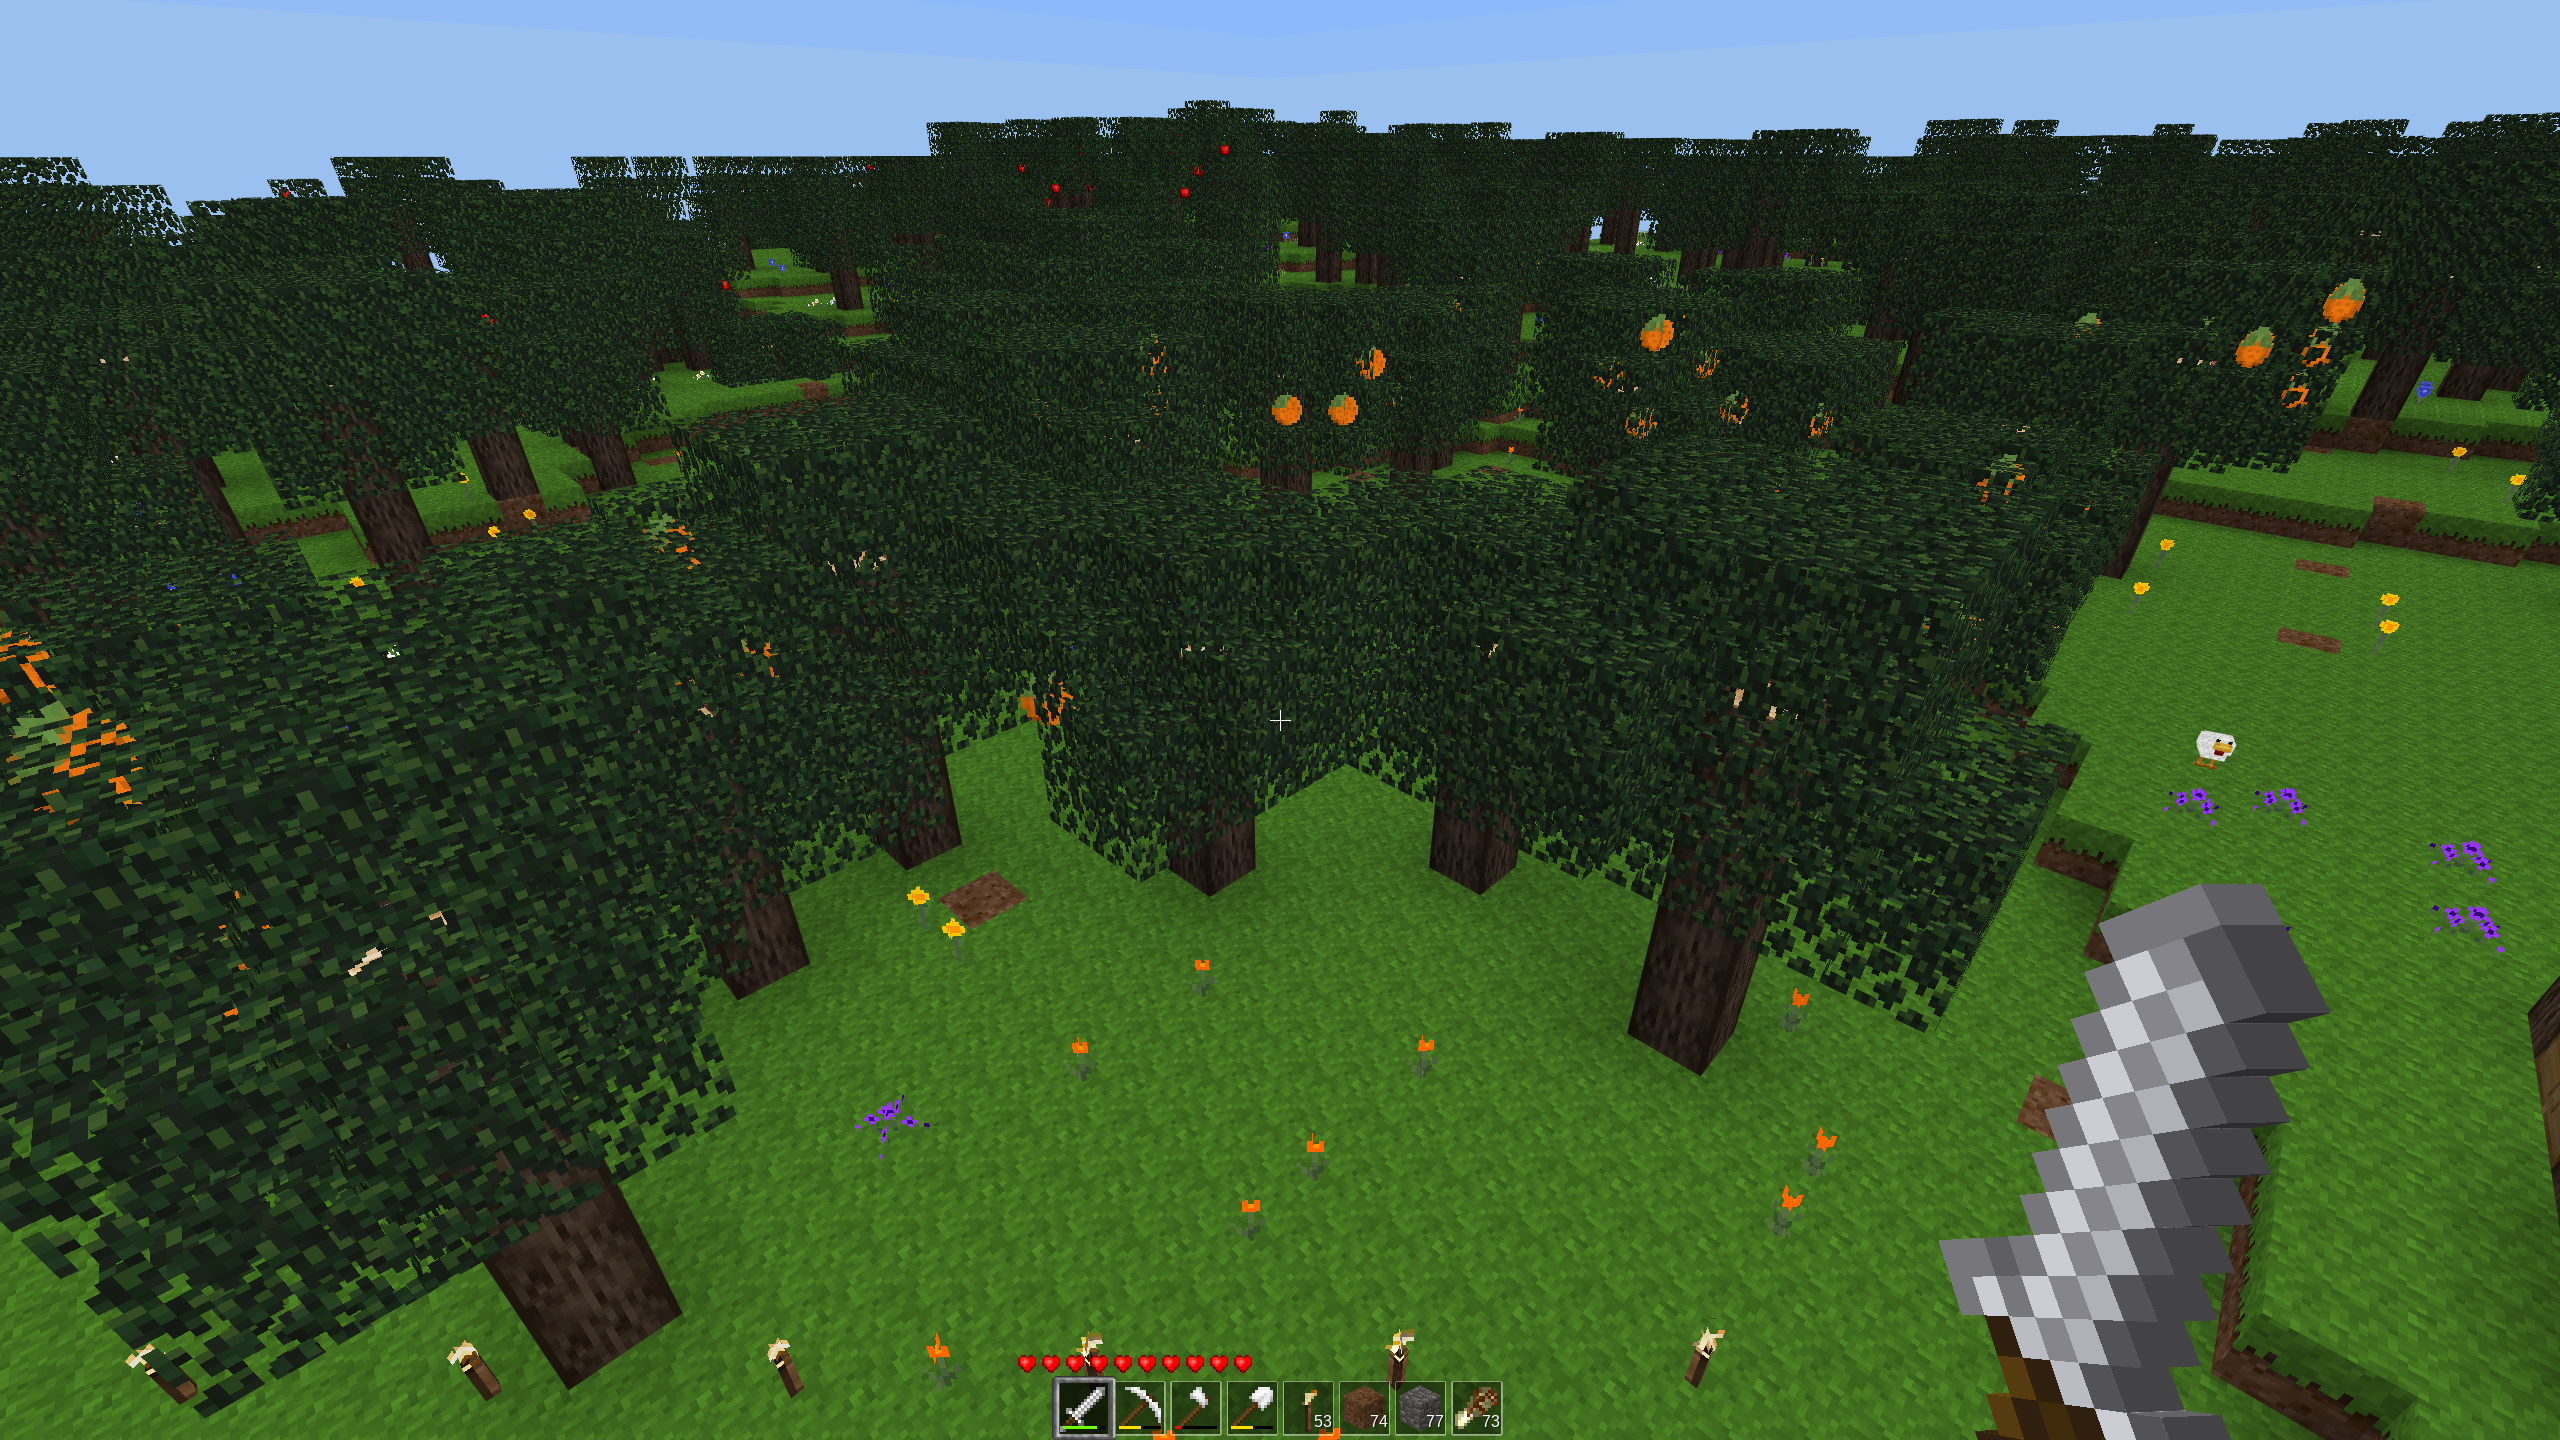
\includegraphics[scale=0.33]{files/blog/2019_03_31_tree_growth_in_minetest/2019_03_31_orange_trees.png}
\caption{A group of orange trees (with regular trees behind them) before harvest.}
\end{figure}

As I began to grow and harvest an orchard of the extra trees I began to notice that sometimes a tree would grow near-instantaneously while others would languish for what seemed to be an indefinite time.

\begin{figure}
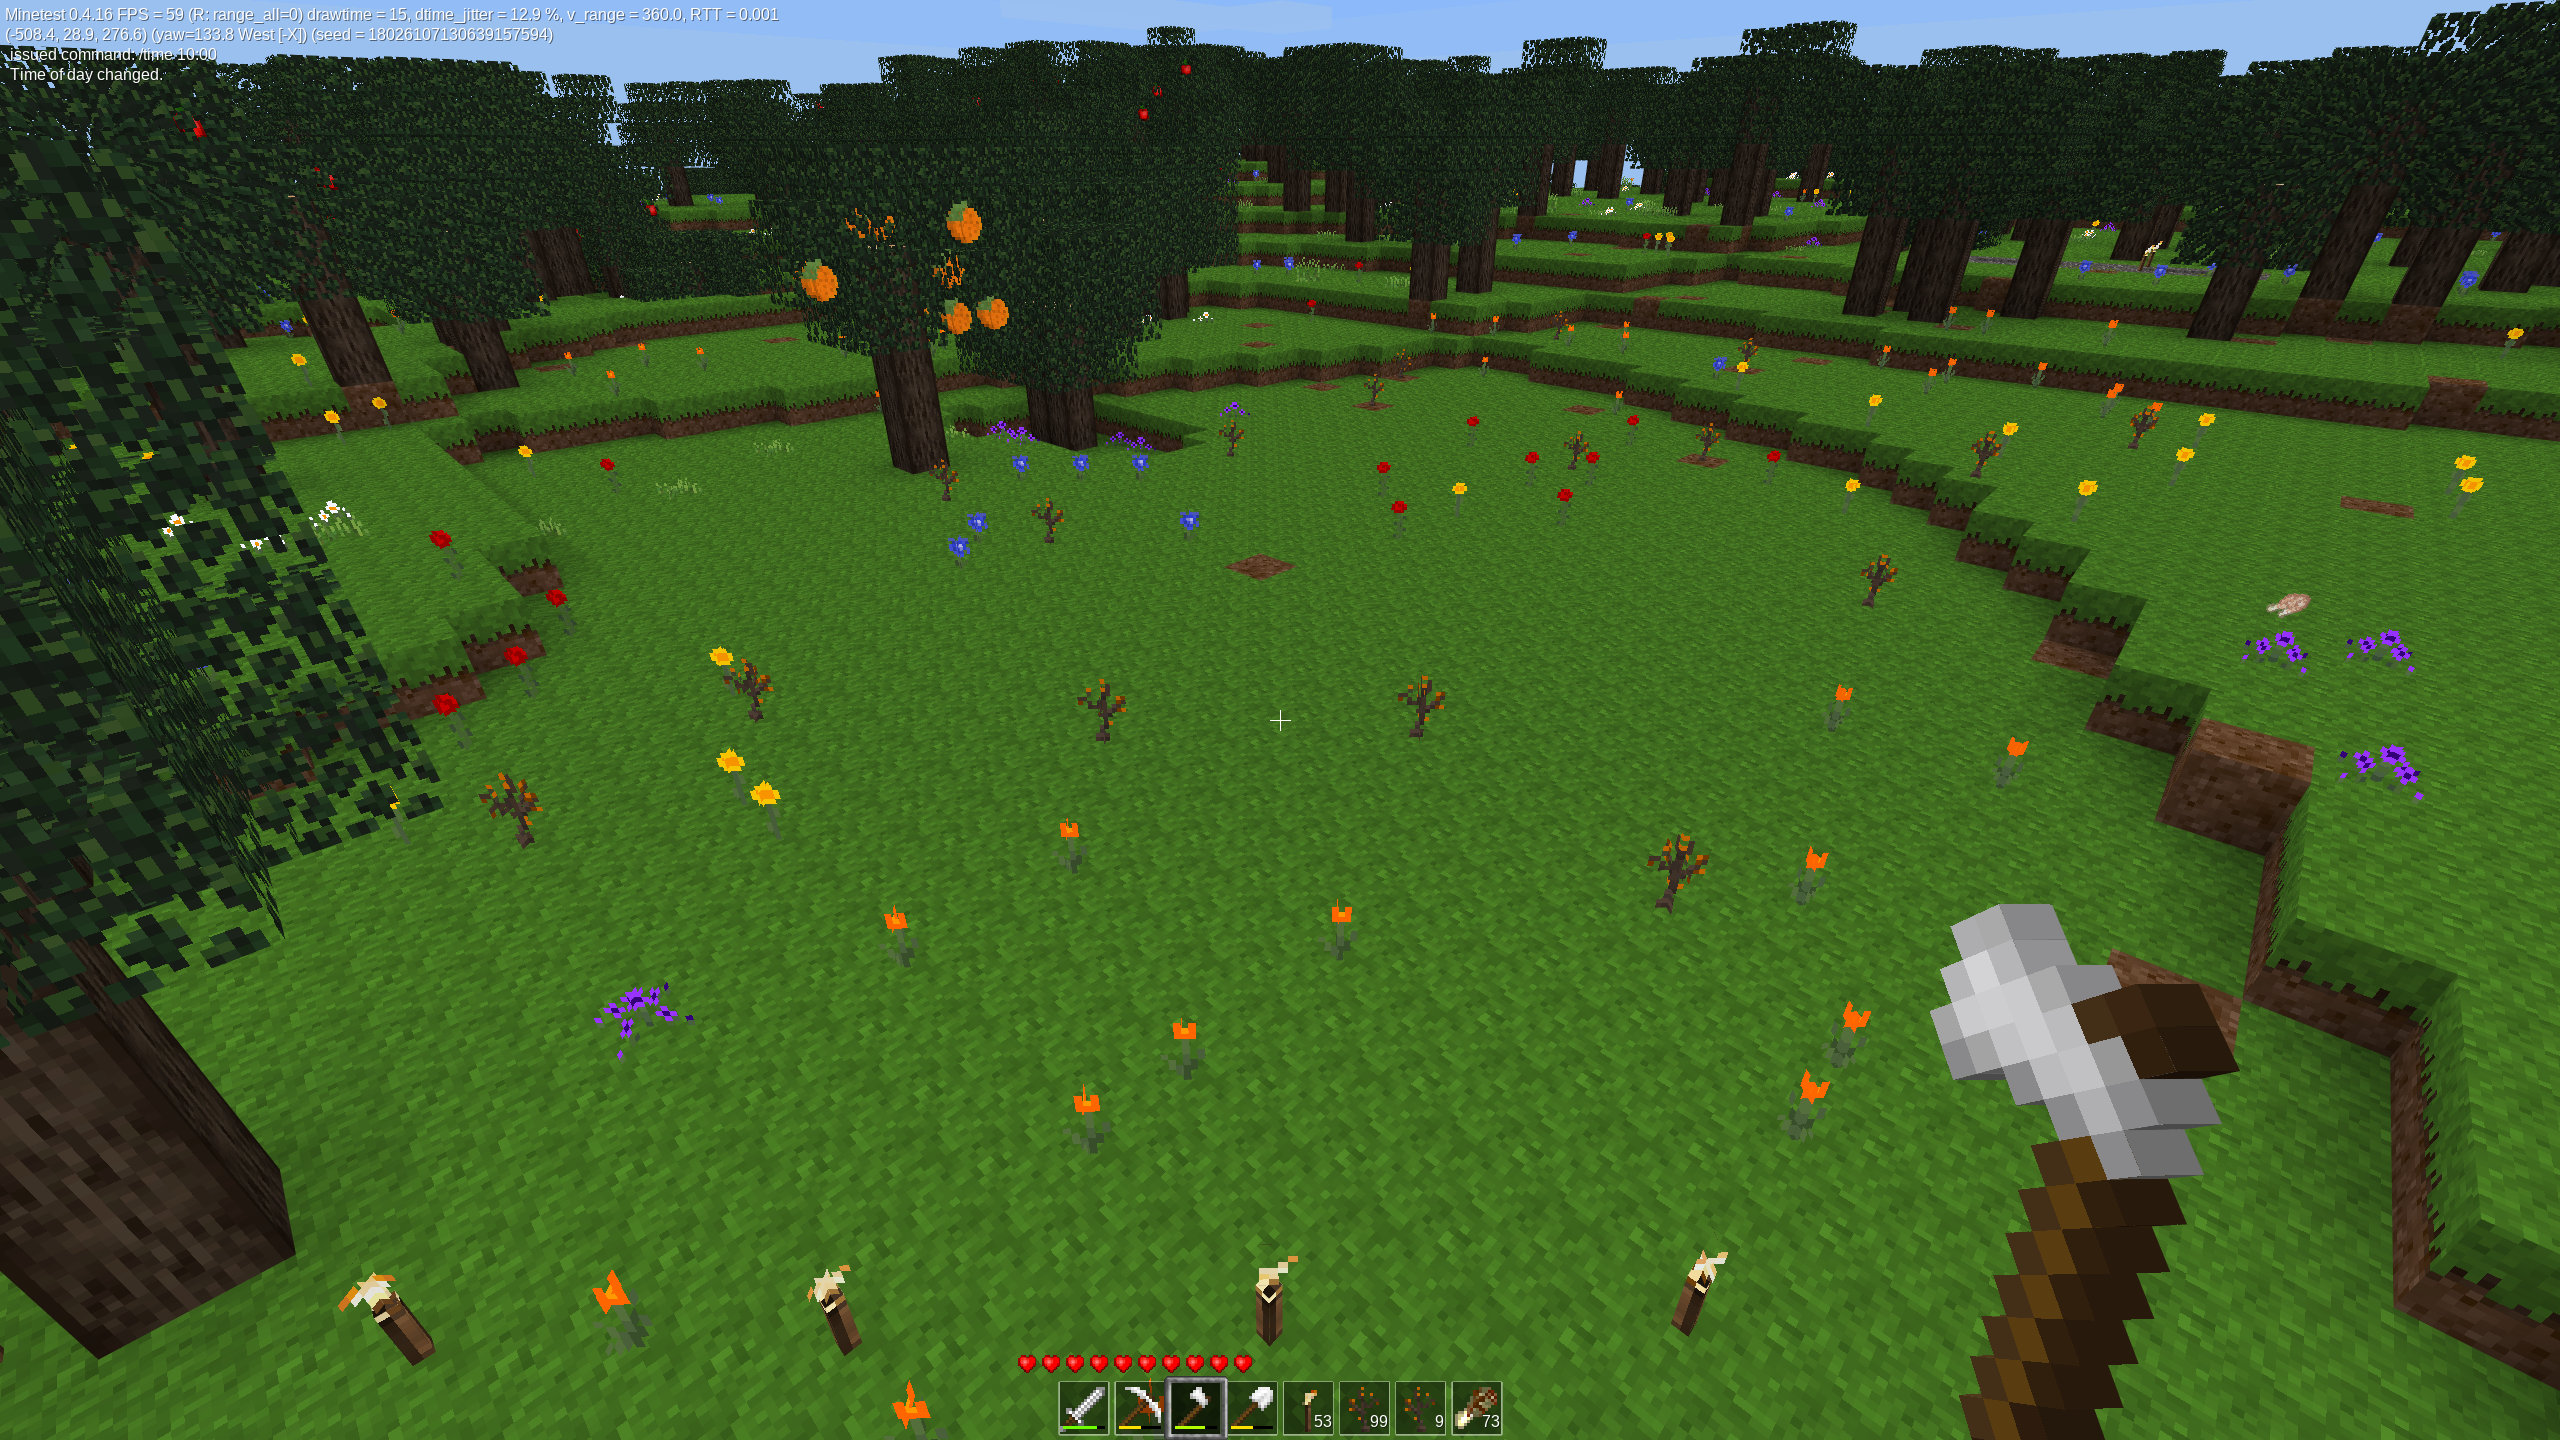
\includegraphics[scale=0.33]{files/blog/2019_03_31_tree_growth_in_minetest/2019_03_31_harvested.png}
\caption{Immediately after being harvested and re-planted, one of the saplings has already grown into a tree.}
\end{figure}

The trees in the default game, however, seemed to grow at a steady rate.  The growth asymmetry bothered me, so I decided to study and modify the code so that the mod would match the default game.  Note, however, that I wrote the mod against the v0.4.16 version while v5.0.0 (v0.5.0 and company were skipped) is the latest at the time of this posting, so some information may be slightly dated.

\subsection{Active Block Modifiers}
The first thing I learned was that the mod's trees were using something called an Active Block Modifier (ABM) in order to trigger their growth.  The idea is pretty simple: after a certain amount of time has passed then the tree has a chance to grow.  If it doesn't grow, it waits the same amount of time again before again having the same chance to grow, ad infinitum.  An example definition is as follows:
\begin{verbatim}
	minetest.register_abm({
	        nodenames = {"farming_plus:orange_sapling"},
	        interval = 60,
	        chance = 20,
	        action = function(pos, node)
	                farming_plus.generate_tree(pos, "farming_plus:orange_tree", "farming_plus:orange_leaves", {"default:dirt", "default:dirt_with_grass"}, "farming_plus:orange", 20)
	        end
	})
\end{verbatim}
\texttt{nodenames} are the nodes affected by the ABM, the amount of time that has to pass is the \texttt{interval}, the likelihood of growing is the \texttt{chance}, and the function for growing the tree is the \texttt{action}.  The interval is measured in seconds, while the chance is actually an inverse value, that is, the chance is measured as 1 divided by the value of chance.  For the mod's tree growth, the value of the interval was 60, meaning the tree had a chance to grow every minute, and the value of chance was 20, meaning there was a 1 in 20, or 5\%, chance that it would grow; thus each tree had a 5\% chance to grow every minute.  So, when I'd harvest 20+ trees over a few minutes it was no wonder that a few would grow while I was still harvesting them.

\subsection{Node Timer}
Having learned how the mod was growing trees, I dug into the game's source code (technically the source code for the \texttt{default} mod in \texttt{minetest_game}, not the Minetest source code itself) and found in \texttt{mods/default/trees.lua} that the default trees were using a Node Timer object for growth.  This per-node object allows one to trigger a function callback after a certain time period.  In order to add the timer's callback to my saplings I modified the \texttt{register_node} function which created my saplings to include an \texttt{on_timer} field whose value was the callback function for growth; in addition, I added an \texttt{on_construct} field which would start the timer when the tree's corresponding sapling was placed (constructed) with a randomized interval (with min and max values taken from the default trees).  The additions thus looked like:
\begin{verbatim}
	minetest.register_node("farming_plus:orange_sapling", {
		...
	        on_timer = function(pos)
	                farming_plus.generate_tree(pos, "farming_plus:orange_tree", "farming_plus:orange_leaves", {"default:dirt", "default:dirt_with_grass"}, "farming_plus:orange", 20)
	        end,
	        on_construct = function(pos)
	                minetest.get_node_timer(pos):start(math.random(2400,4800))
	        end,
	})
\end{verbatim}
This meant that trees would then grow after 40 to 80 minutes (2400 to 4800 seconds, respectively), making growth generally much longer than the previous duration but also normalizing the growth rate.  There's a caveat, though: suppose that the \texttt{on_timer} function is called but the tree doesn't grow because it's too dark out or some other reason.  In that case the timer would be deactivated and the tree would never grow even if conditions changed; this meant that it was necessary to also reset the timer in the \texttt{generate_tree} function (again, using the values from the default trees):
\begin{verbatim}
        if cant_grow then
                minetest.get_node_timer(pos):start(math.random(240, 600))
                return
        end
\end{verbatim}
In this case \texttt{cant_grow} is a bool which, obviously, has been set based on whether or not the tree can grow.

So far, both newly-created saplings and saplings with bad growth conditions are covered, but there's one more rather subtle case left uncovered: saplings which were created before the change to timer-based growth were made.  It turns out that the timer definition actually applies to saplings retroactively, but the timer isn't activated and so they will never grow!  In order to combat this I applied something called a Loading Block Modifier (LBM); what this does it that, each time an area with the specified nodes (in this case, saplings) is loaded, the specified action is applied to those nodes (in this case, causing the saplings to grow into their corresponding tree).  Hence, I added the following code:
\begin{verbatim}
	minetest.register_lbm({
	        name = "farming_plus:sapling_growth",
	        nodenames = {"farming_plus:banana_sapling",
	                "farming_plus:cocoa_sapling",
	                "farming_plus:cherry_sapling",
	                "farming_plus:orange_sapling"},
	        run_at_every_load = true,
	        action = function(pos)
	                local timer = minetest.get_node_timer(pos)
	                if timer:is_started() == false then
	                        timer:start(math.random(2400, 4800))
	                end
	        end
	})
\end{verbatim}
The \texttt{nodenames} field contains each node that will be affected by the LBM, the \texttt{run_at_every_load} field ensures that the LBM will actually be run for current blocks, and the \texttt{action} is the function to run on the loaded blocks.  The important thing here is not to interfere with saplings whose growth timer has already been started.  Thankfully, the timer provides an \texttt{is_started} method in order to check this; if the timer is not started, then, since older saplings will regardless have the growth timer attached to them, simply start the timer with the usual values.  Interestingly enough, the game engine, as of this writing, works in such a way that: the timer is started, the time since the last load of the area is calculated, and then the time past is decremented from the timer.  What this means is that a sapling may be triggered on the first load of an area if sufficient time has passed, rather than the first load simply triggering the timer and the corresponding wait.  That's pretty satisfying, actually.

\subsection{Comparison}
It's worth comparing the growth chance of the two methods with respect to time.  A graph of the methods with their corresponding values is as follows (assuming ideal growing conditions):

\begin{figure}
\includegraphics{files/blog/2019_03_31_tree_growth_in_minetest/2019_03_31_growth.png}
\end{figure}

The values used in both the ABM and Node Timer methods predispose the ABM method to early growth, but what's important here is actually the \emph{shape} of the two methods' rate.  As you can see, the ABM method has a chance of ultra-early growth and a slight chance of ultra-late growth.  The Node Timer method, on the other hand, has no chance of early or late growth.  This will be the case for both growth methods regardless of the values used for growth time.  As stated before, I prefer the latter due to its consistency.

\subsection{Conclusion}
Thus the transition from ABMs to Node Timers was complete, and tree growth was now consistent between the mod and the default game.  The commit can be found \htmladdnormallink{here}{https://github.com/clinew/farming_plus/commit/087127f2bc6e55cd15226e15e576a5f72a2741ca} (astute readers may notice a discrepancy between the date of the commit and this blog; indeed, I had created the initial version of the patch on my local copy of the repo at the date of the patch, but did not fix the LBM bug it had and publish it until recently).  Now, hopefully when I migrate to the newer game version nothing will break\ldots


% Pillars of Eternity: Path of the Damned, Act IV
\section{2019-03-17 Pillars of Eternity: Path of the Damned, Act IV}
I was lying about jumping down the pit next.  First, I had some unfinished business with Lord Gathbin, followed by a brutal fight with the Master Below, before actually jumping down the pit towards Thaos.

% Army fight
\subsection{Lord Gathbin}
I saved this fight until near-endgame.  Partially because it's not really clear when to do it, but also because I wanted to use the massive army as target practice at a high level.  Due to a weird alliance bug in the game, the spell-casters started out by attacking each other while I buffed myself.

\begin{figure}
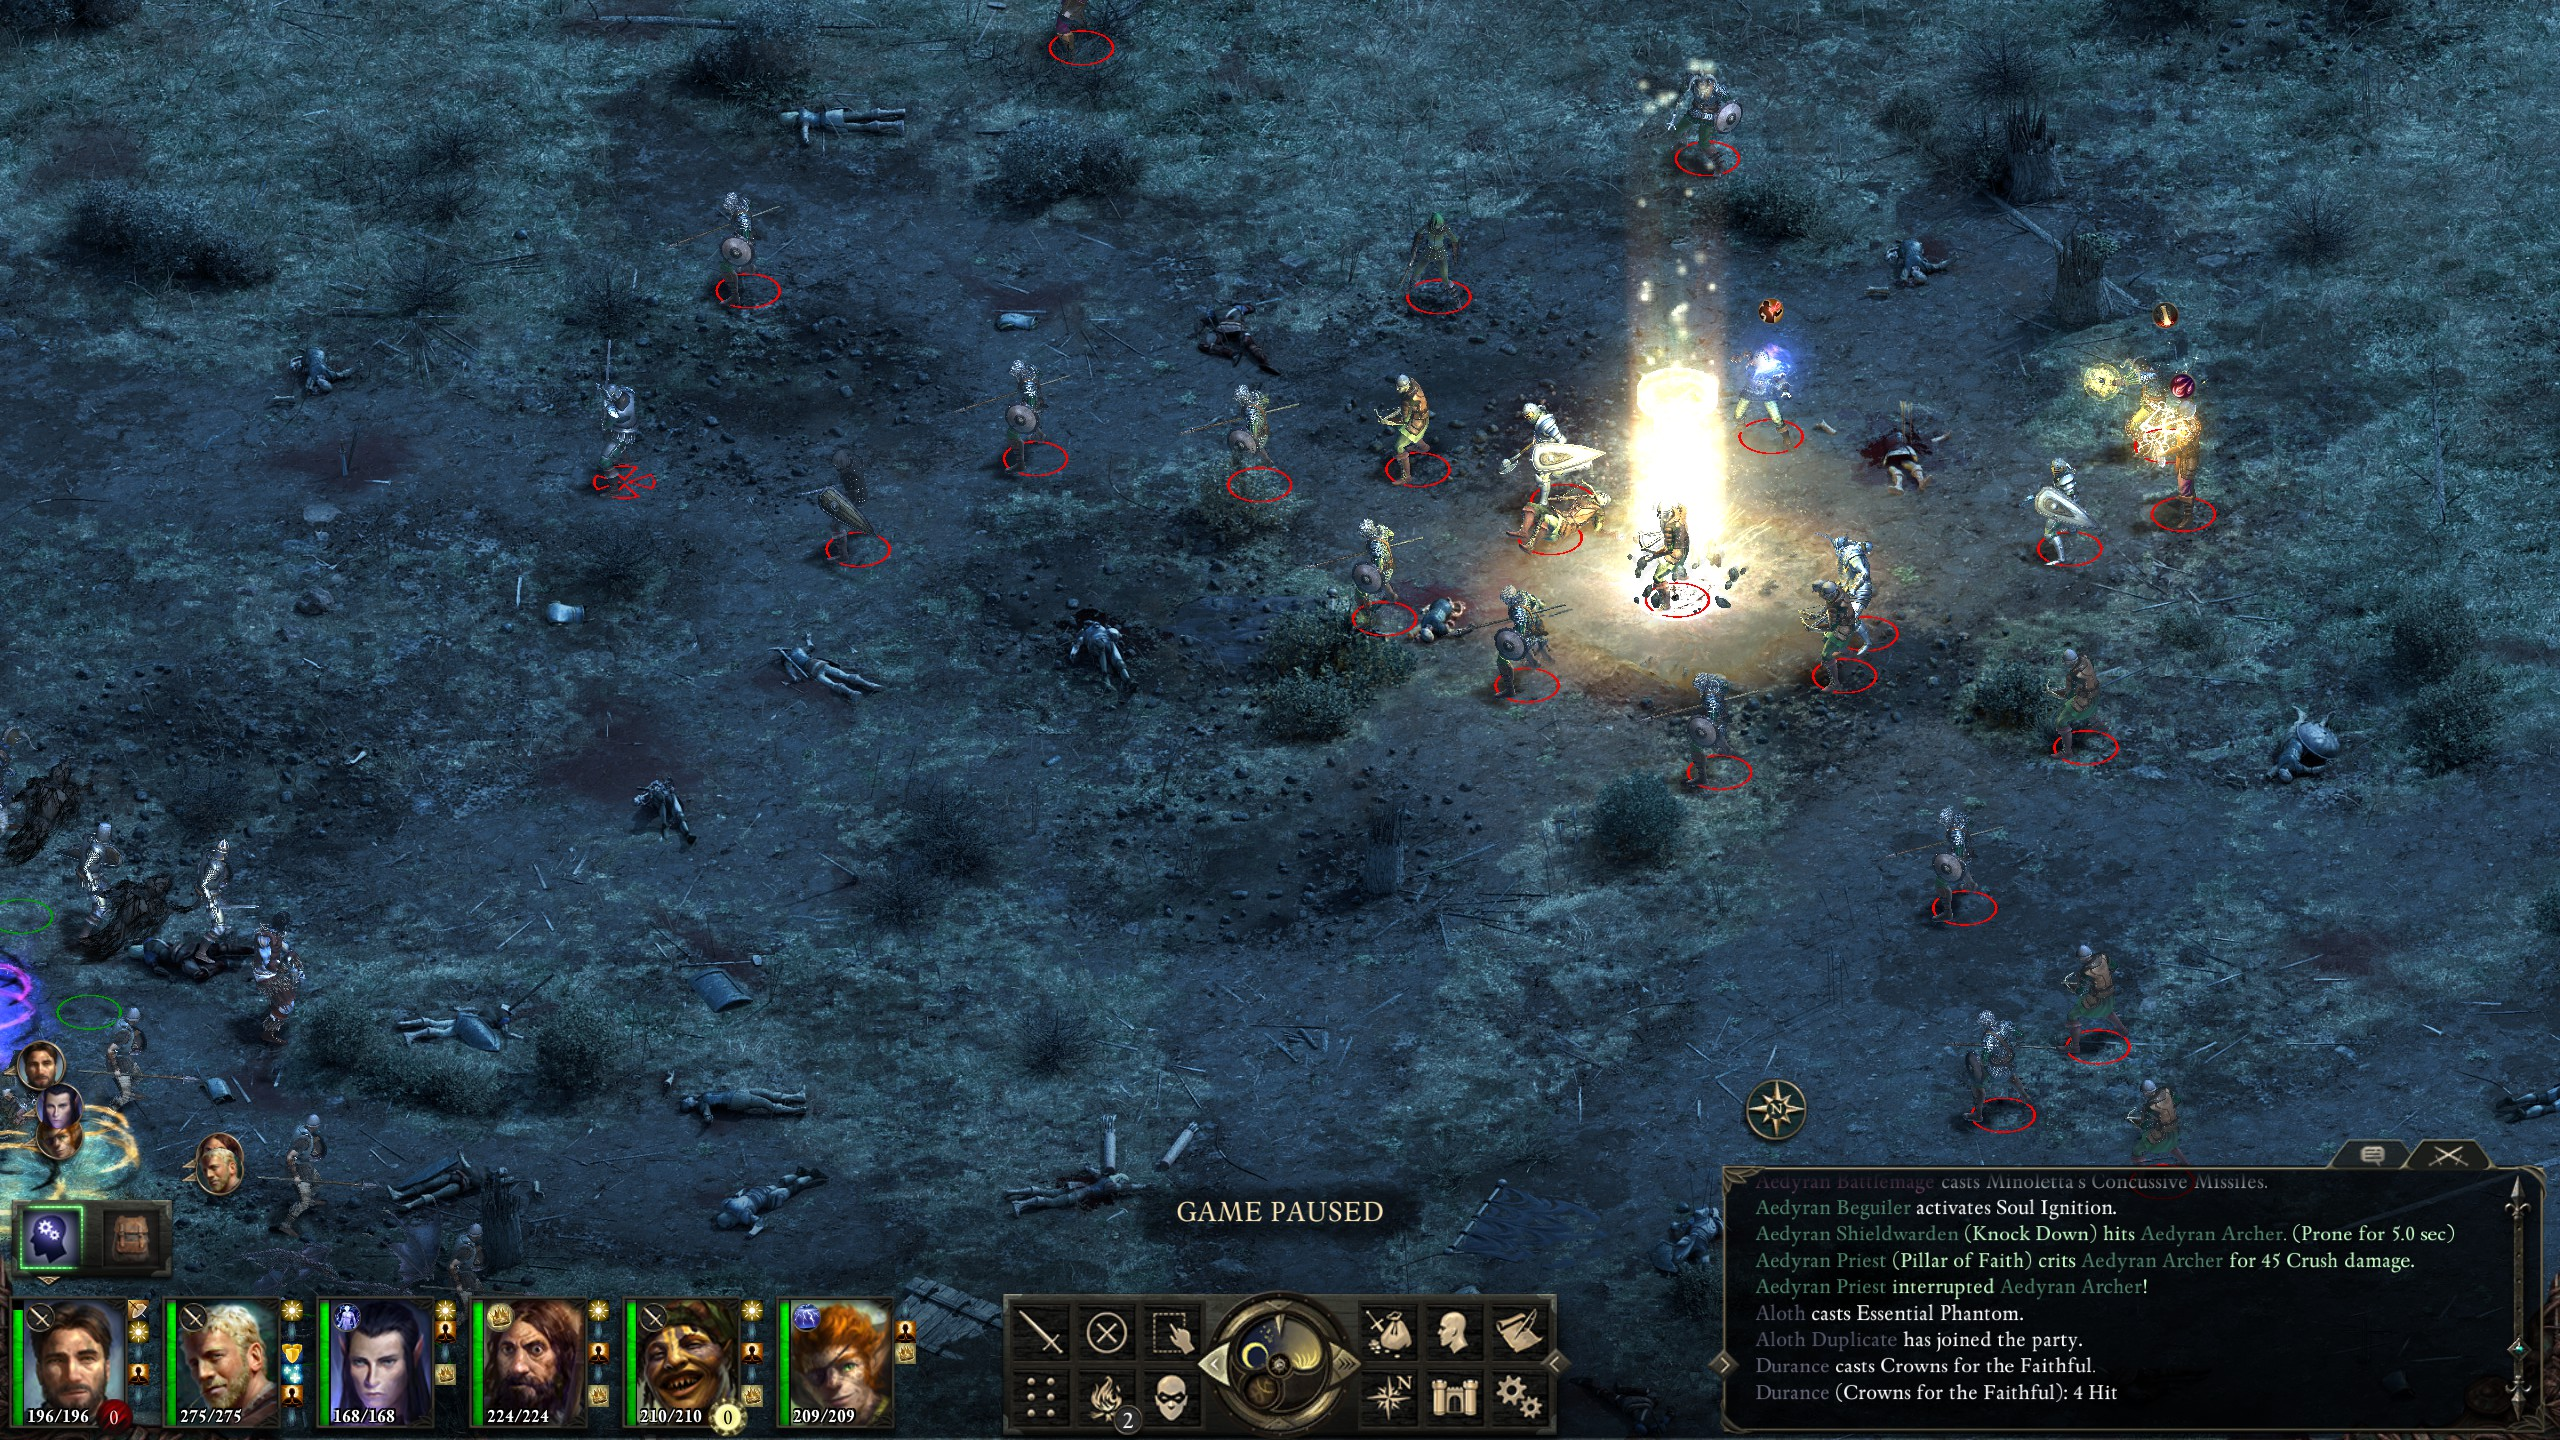
\includegraphics[scale=0.33]{files/blog/2019_03_17_pillars_of_eternity_path_of_the_damned_act_iv/2019_03_17_gathbin1.jpg}
\end{figure}

It didn't help them against the coming steamroll.

\begin{figure}
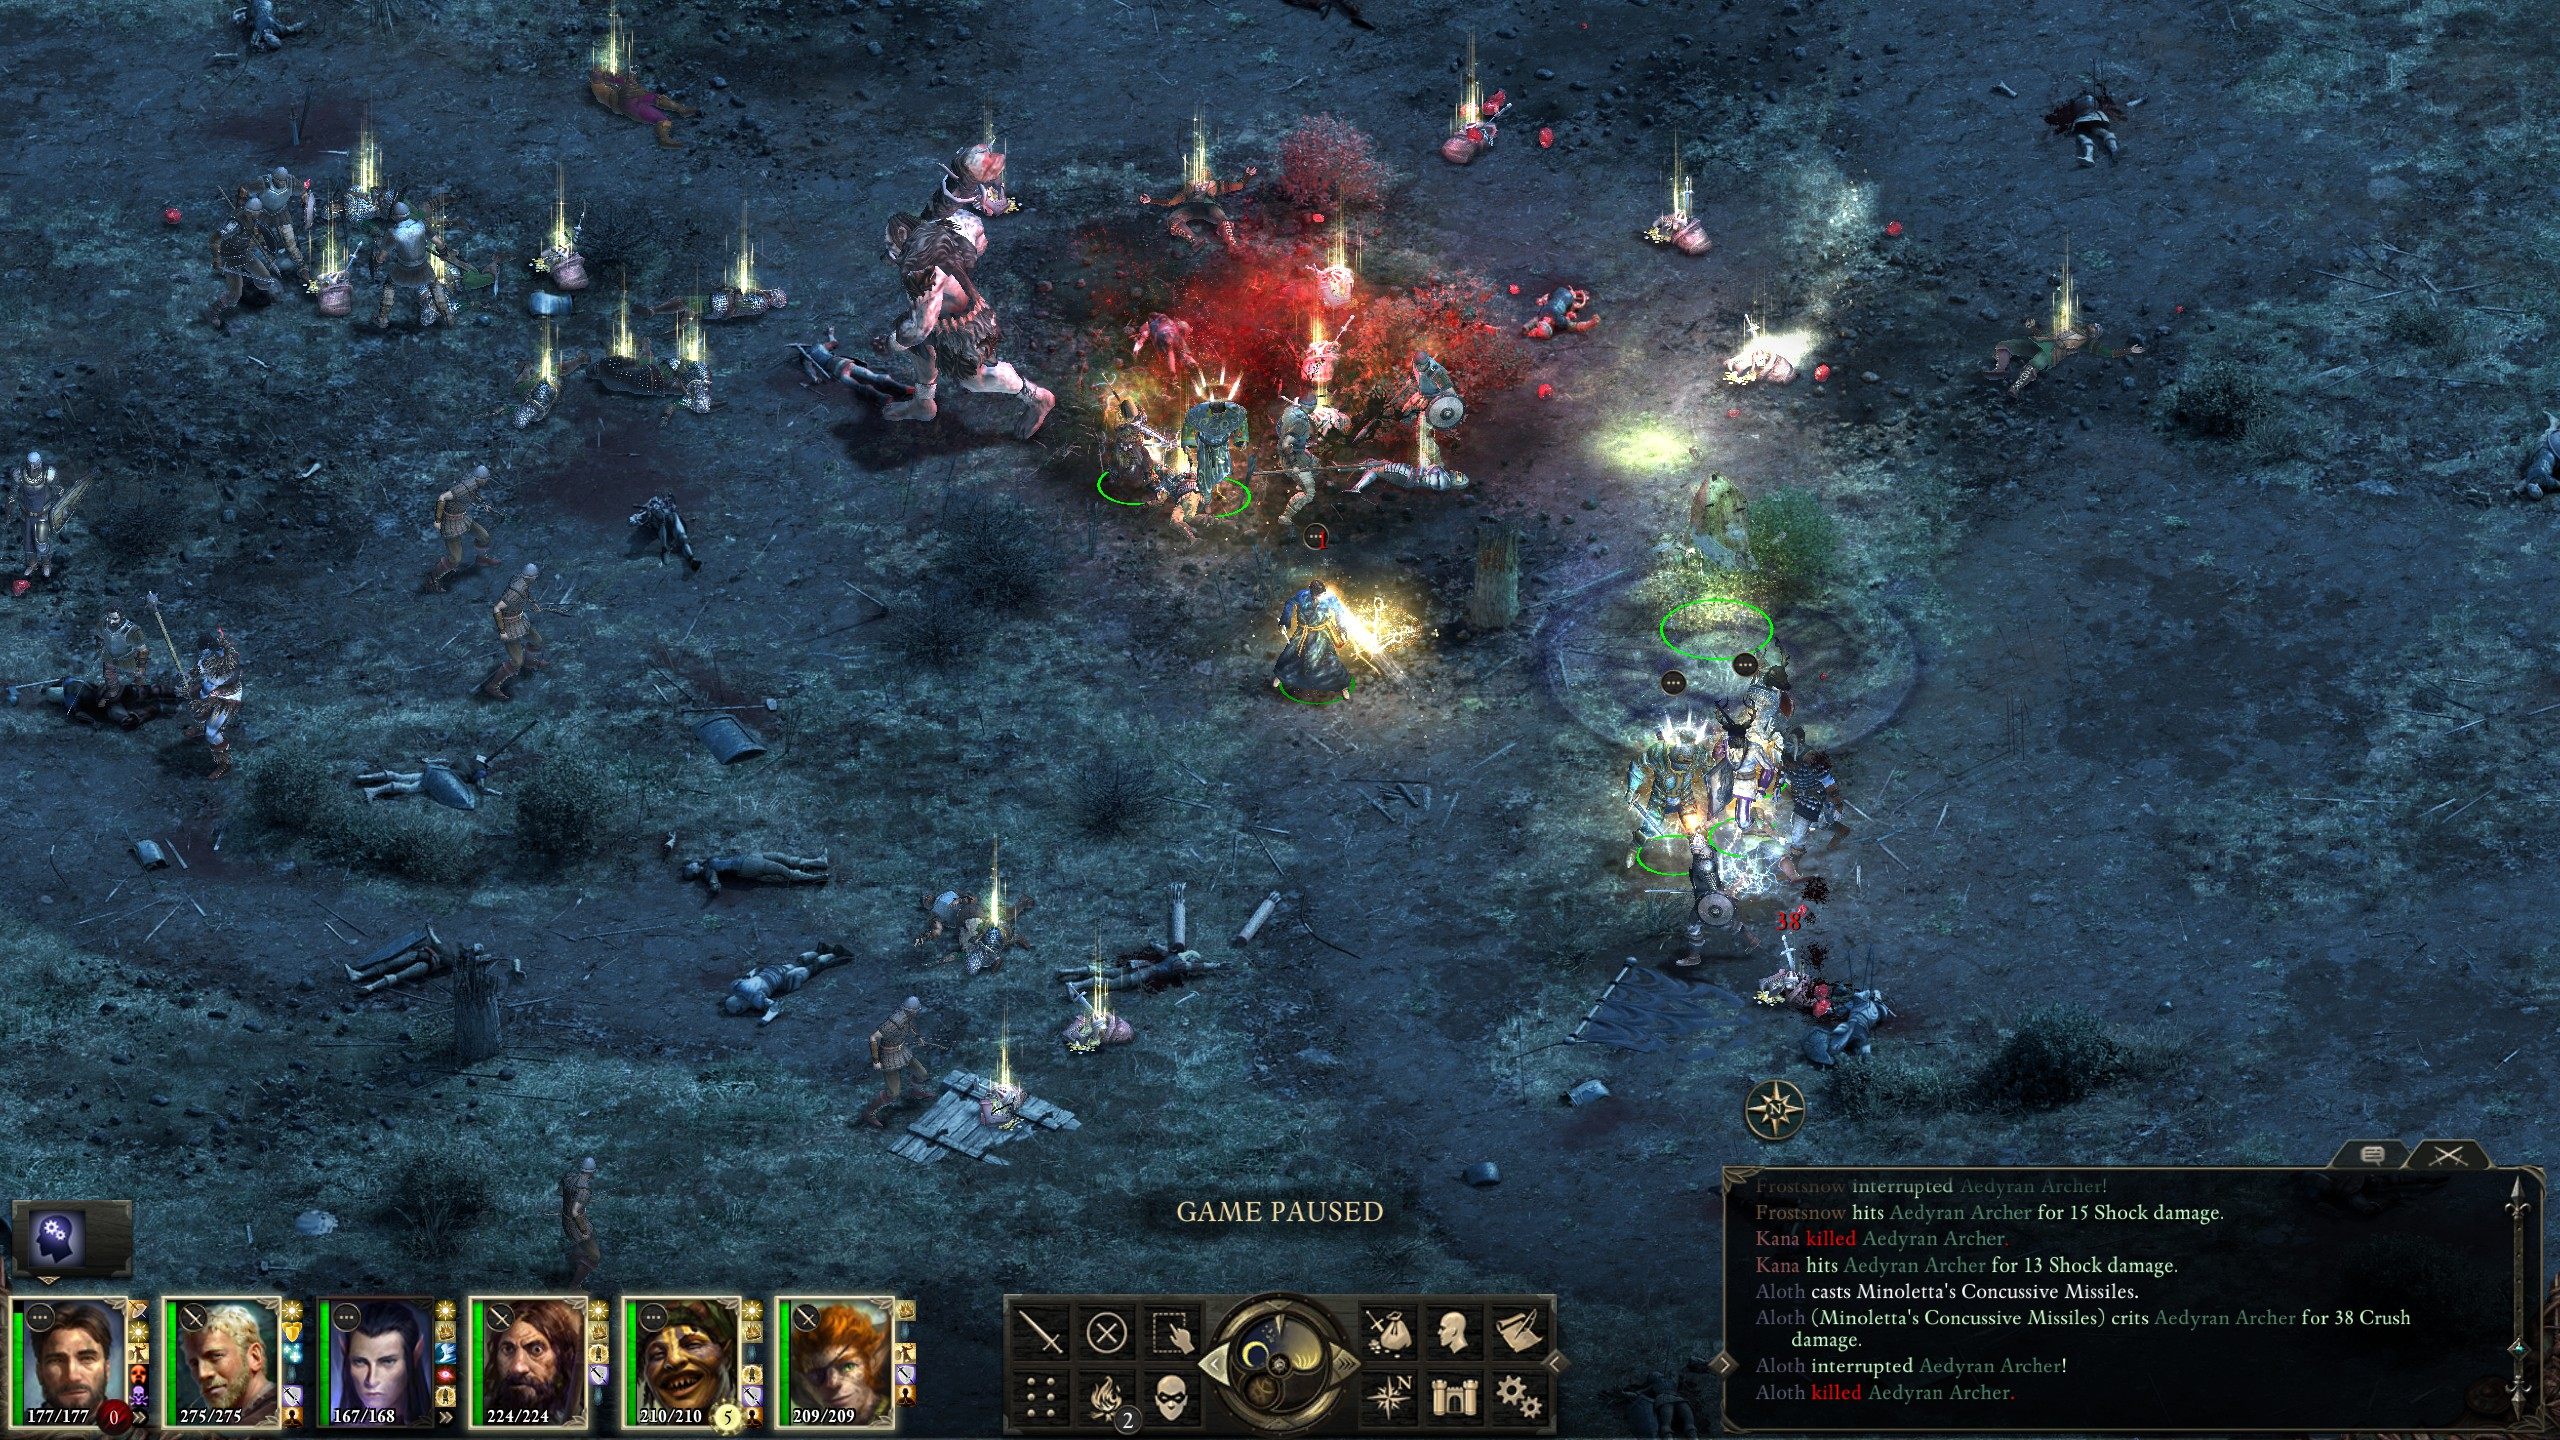
\includegraphics[scale=0.33]{files/blog/2019_03_17_pillars_of_eternity_path_of_the_damned_act_iv/2019_03_17_gathbin2.jpg}
\end{figure}

I actually didn't get any really cool combinations off as the enemies were all too far apart.  Nonetheless, they were easily smashed, a nice warm-up for the next fight...

\subsection{The Master Below}

The single most challenging fight in the game: the Master Below, who, spoiler alert, is an Adra Dragon.  My very first encounter on "Normal" mode with this dragon was such a disaster that I didn't play for three days, though I'd been easily crushing all my other foes.  The dragon itself hits hard, and it has two special abilities which hit even harder in an area in front of it: Wing Slam and Breath; the first has the added effect of knocking characters down, and the second simply hits with tons of corrode damage.  Then the adds start coming.  There are adragans which have dominate and petrify abilities and a miniature horde of xaurips with their paralyzing spears.  Combined with the dragon itself the fight is thus extremely difficult.  Preparations were in order.

\subsubsection{Preparations}

Equipping gear is an obvious enough optimization; I've always done it, and I'm not going to go into detail about it here, but this time I decided to take it a step further and see what I could do with consumables.  I crafted or bought the following potions and distributed them amongst my party:

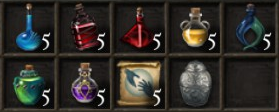
\includegraphics{files/blog/2019_03_17_pillars_of_eternity_path_of_the_damned_act_iv/2019_03_17_potions.png}

\begin{itemize}
	\item Potion of Deleterious Alacrity of Motion
	\item Flask of War Paint
	\item Potion of Merciless Gaze
	\item Potion of Major Recovery
	\item Potion of Llengrath's Displaced Image
	\item Potion of Bulkwark Against the Elements
	\item Potion of Major Endurance
\end{itemize}
In addition I crafted a few "Scrolls of Revival" for Aloth and gave Hiravas "Remembrance Ashes" so that they could both cast revives.  Then it also occurred to me that, since I'd need all the power I could muster, that I could also craft food for its meager bonuses.  I looked through the list of craftables and generated the following list:

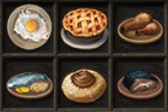
\includegraphics{files/blog/2019_03_17_pillars_of_eternity_path_of_the_damned_act_iv/2019_03_17_food.png}

\begin{itemize}
	\item Farmer's Spread
	\item Rauatai Sweet Pie
	\item Pearlwood Chicken
	\item Casita Casserole
	\item Darkest Rauatai Cookie
	\item Dragon Meat Dish
\end{itemize}
With all of these items I had:
\begin{itemize}
	\item +3 Might
	\item +2 Dexterity
	\item +2 Constitution
	\item +2 Intelligence
	\item +1 Perception
	\item +3 Resolve
	\item +45 Max Endurance
	\item +5 Max Health
	\item +1 Move Speed
\end{itemize}
It turned out that all of the food bonuses combined are actually quite powerful!  If I'd paid a bit more attention, though, I might have noticed that I didn't need the "Pearlwood Chicken" and I could have added an "Ale" for an extra +2 Damage Reduction.  Alas, hindsight is 20/20, and by the time I reached this level of ricing, I'd already spent 3 and a half hours preparing.  Ricing isn't enough, though; a strategy was needed as well.

A big problem with the dragon is its Wing Slam and Breath attacks, which hit everyone in a cone in front of it.  The first and most obvious way to counter this is to go behind it in order to get both flanking bonuses and avoid its breath attacks; this, in fact, does not work, because it has a tail attack that does even \emph{more} damage, enough to knock out my main tank with one blow.  Ouch.  Astute players may note that, since turning is instant in this game, then why doesn't the dragon just turn around and one-shot the tank rather than attack it directly; well, probably because the developers wanted a challenging but fair fight so they don't have the dragon do that, though it is a bit weird from an immersion perspective.  Nonetheless, directly flanking does not work.  The next thing one might try is having the ranged characters run away from the dragon when it begins to do such an attack and let the melee characters simply get hit.  The problem here is that I've not found an easy way to do this as the attacks are sudden enough and have enough of a range that running away is often futile.

Flanking was out, and so was backing away, but, after much thought, I finally thought up another trick: two squads 90 degrees apart, with at least one member in each squad having a revive and heals:

\begin{center}
\begin{figure}
\begin{makeimage}
\fbox{ % I don't like this but haven't fixed latex2html's cropping bug yet.
\begin{tikzpicture}
	\draw (0, 0) circle [radius=2];
	\draw[line width=3, color=green, arrows={-Stealth[length=11]}] (-3.5, 0) -- (-2.5, 0);
	\draw[line width=3, color=green, arrows={-Stealth[length=11]}] (0, -3.5) -- (0, -2.5);
	\node [color=red,cross out,draw,line width=3] at (0, 2.5) {};
	\node [color=red,cross out,draw,line width=3] at (2.5, 0) {};
	% Invisible paths help with image alignment since fbox makes it
	% super-obvious.
	\path[line width=3, color=green, arrows={-Stealth[length=11]}] (3.5, 0) -- (2.5, 0);
	\path[line width=3, color=green, arrows={-Stealth[length=11]}] (0, 3.5) -- (0, 2.5);
\end{tikzpicture}
}
\end{makeimage}
\end{figure}
\end{center}

This meant that if one squad got hit with a Breath attack and Wing Slam that the remaining squad could then revive the fallen squad; if the Wing Slam and Breath hit different squads then they should both be able to heal themselves back up to full, and no one would be in a position to get hit by the dragon's deadly tail.  I still needed to deal with the adds, however, so I decided to put Hiravas and my main on the South side and Aloth and Durance on the West side, since Hiravas' Relentless Storm would control the xaurips and Aloth would need to snipe any adragans that came around from the Northwest.  Kana would then tank the South side while Eder tanked the West side.  Strategy in hand, it was time to finally begin the fight.

\subsubsection{Attempt #1}

There's actually one more trick to the battle, and that's getting \emph{into} position, something that I hadn't considered as thoroughly.  This is complicated by the fact that the adragans have a dominate affliction, which, if it hit either of my tanks, could cause chaos with my positioning.  I decided that the best way forward would be to start in a group and have Durance cast "Prayer Against Treachery" while the rest of the team drank "Potions of Major Recovery" in case they got hit with prone, then have them move into position.  The dragon decided to use its Wing Slam.

\begin{figure}
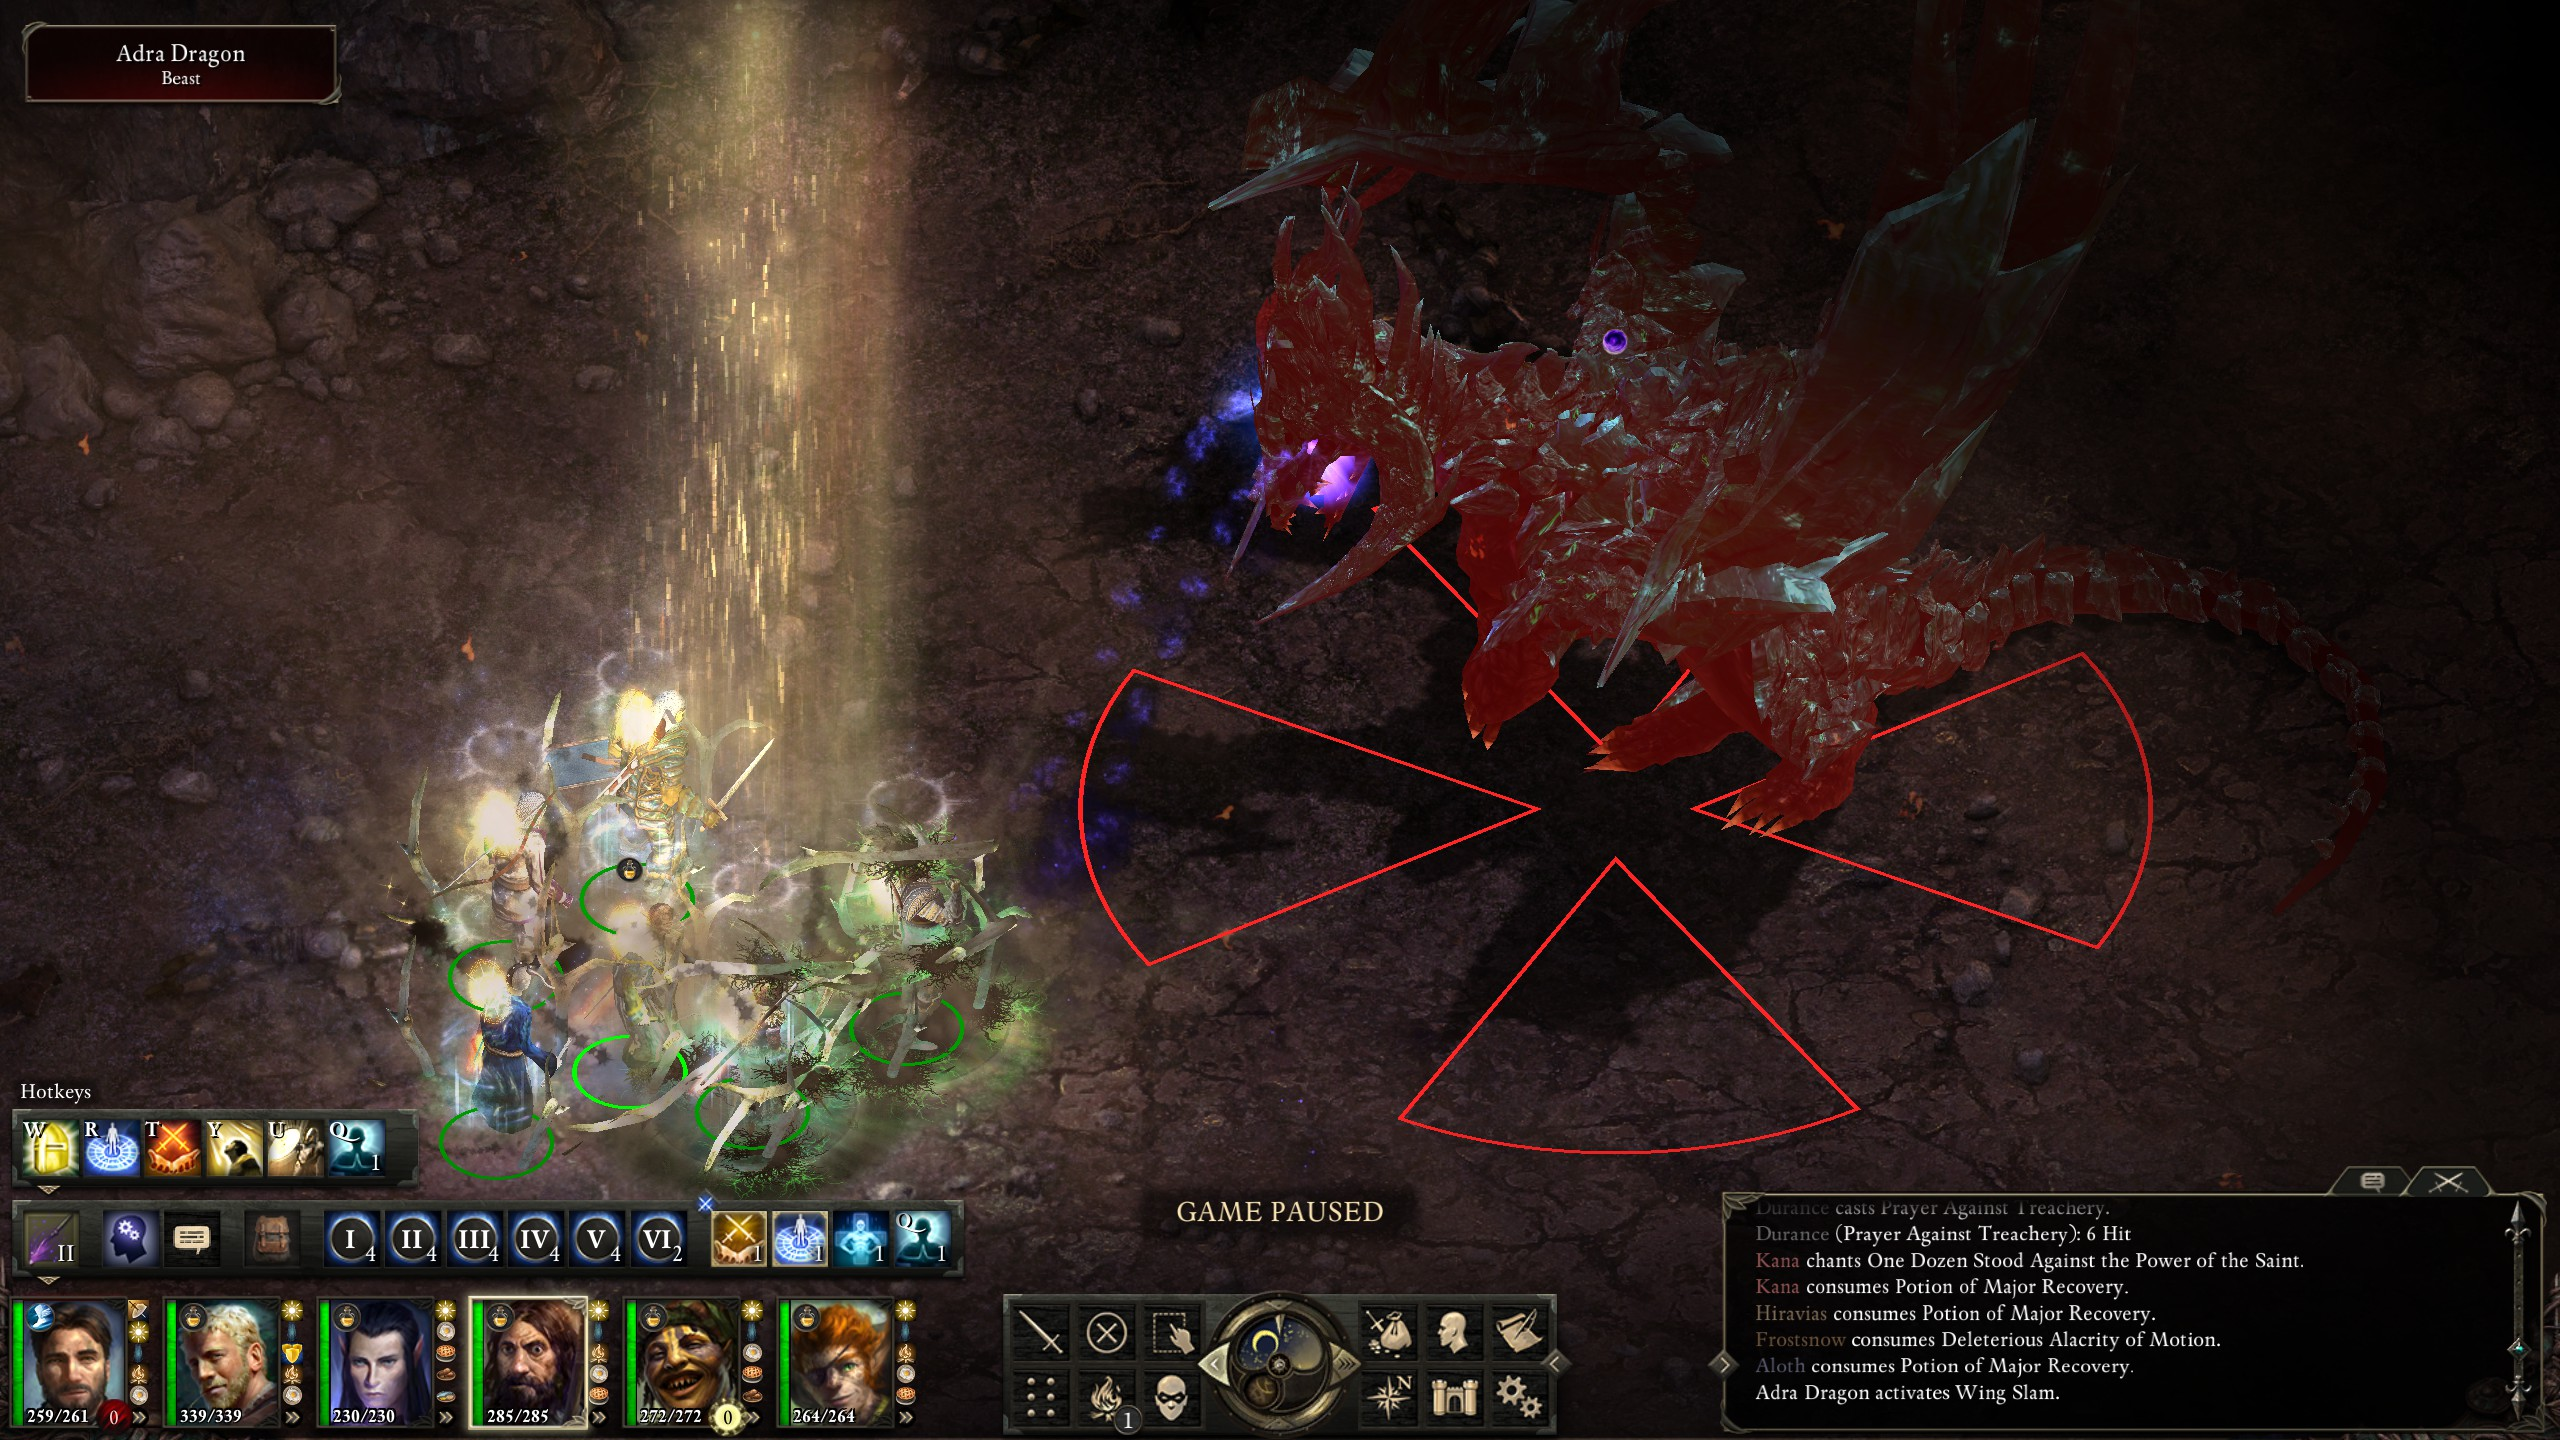
\includegraphics[scale=0.33]{files/blog/2019_03_17_pillars_of_eternity_path_of_the_damned_act_iv/2019_03_17_dragon1_01.jpg}
\end{figure}

The strategy was a disaster; my party was not able drink the potion before the Wing Slam hit, knocking most of them prone.  Before they could get up, the dragon belched out a breath attack.

\begin{figure}
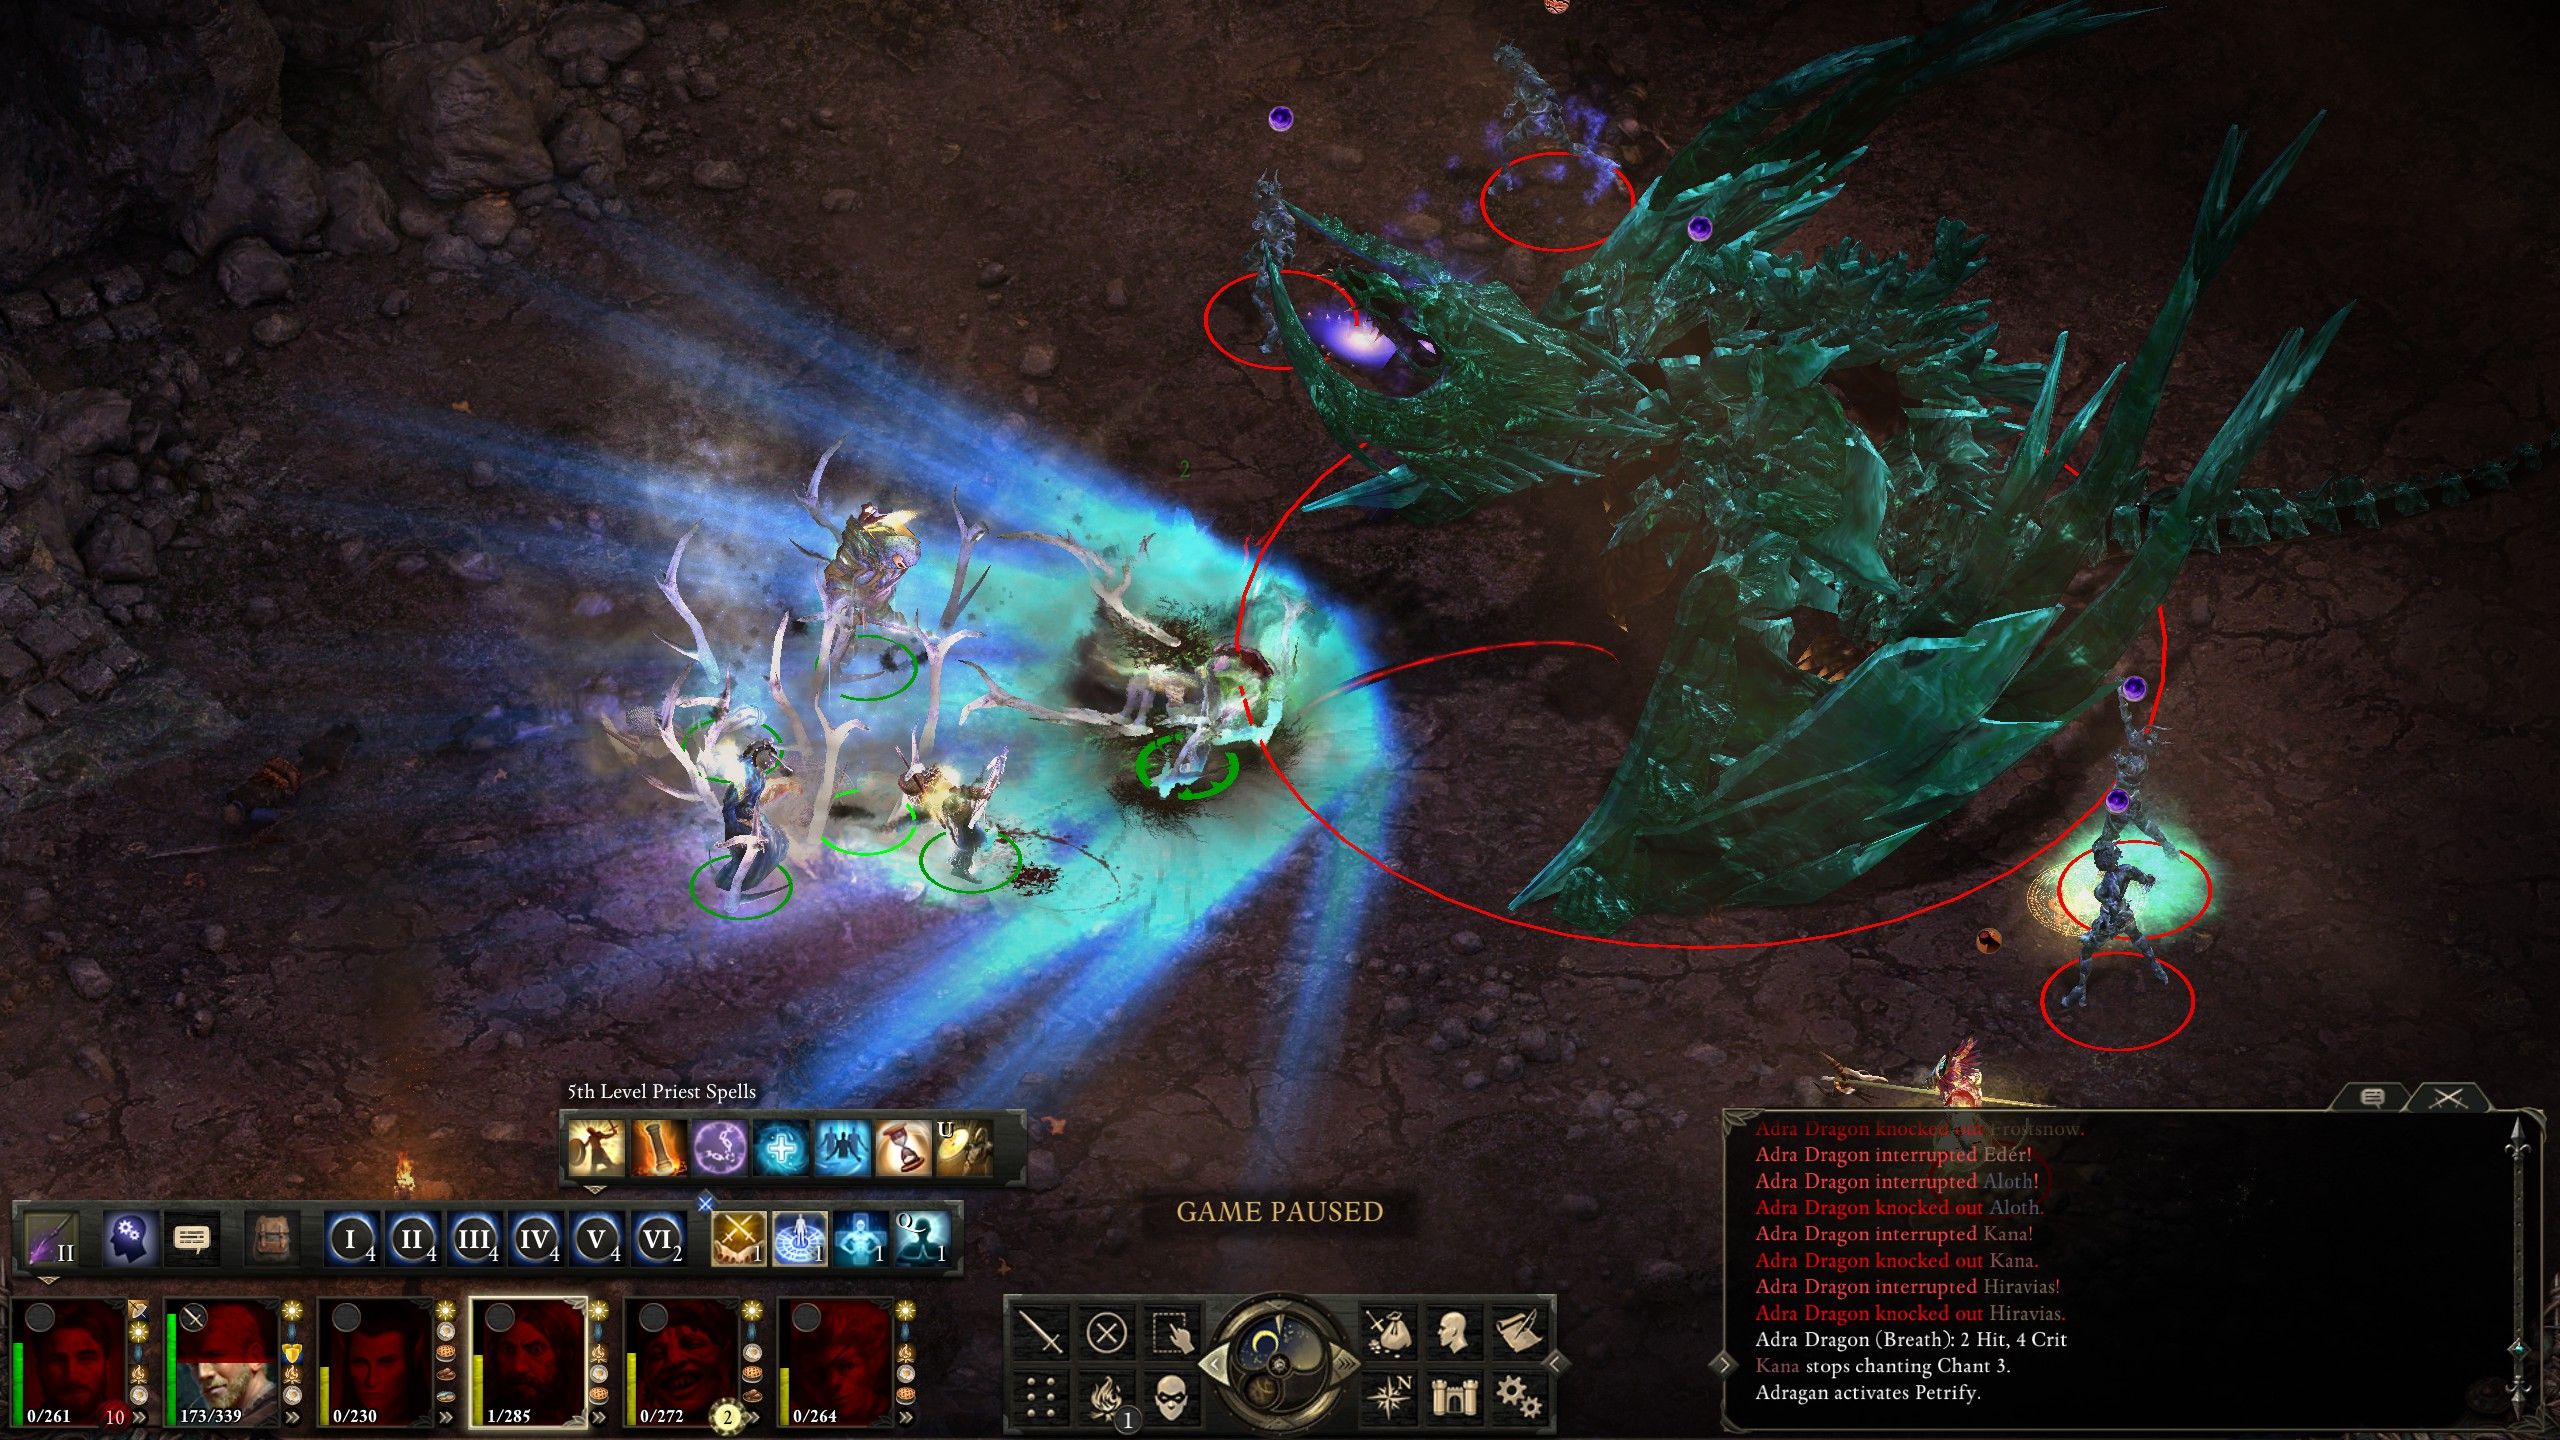
\includegraphics[scale=0.33]{files/blog/2019_03_17_pillars_of_eternity_path_of_the_damned_act_iv/2019_03_17_dragon1_02.jpg}
\end{figure}

Ouch.  Fortunately for me Durance, Hiravas and Kana had items that granted "Second Chance", so I quickly began healing up from what little health I had revived with.

\begin{figure}
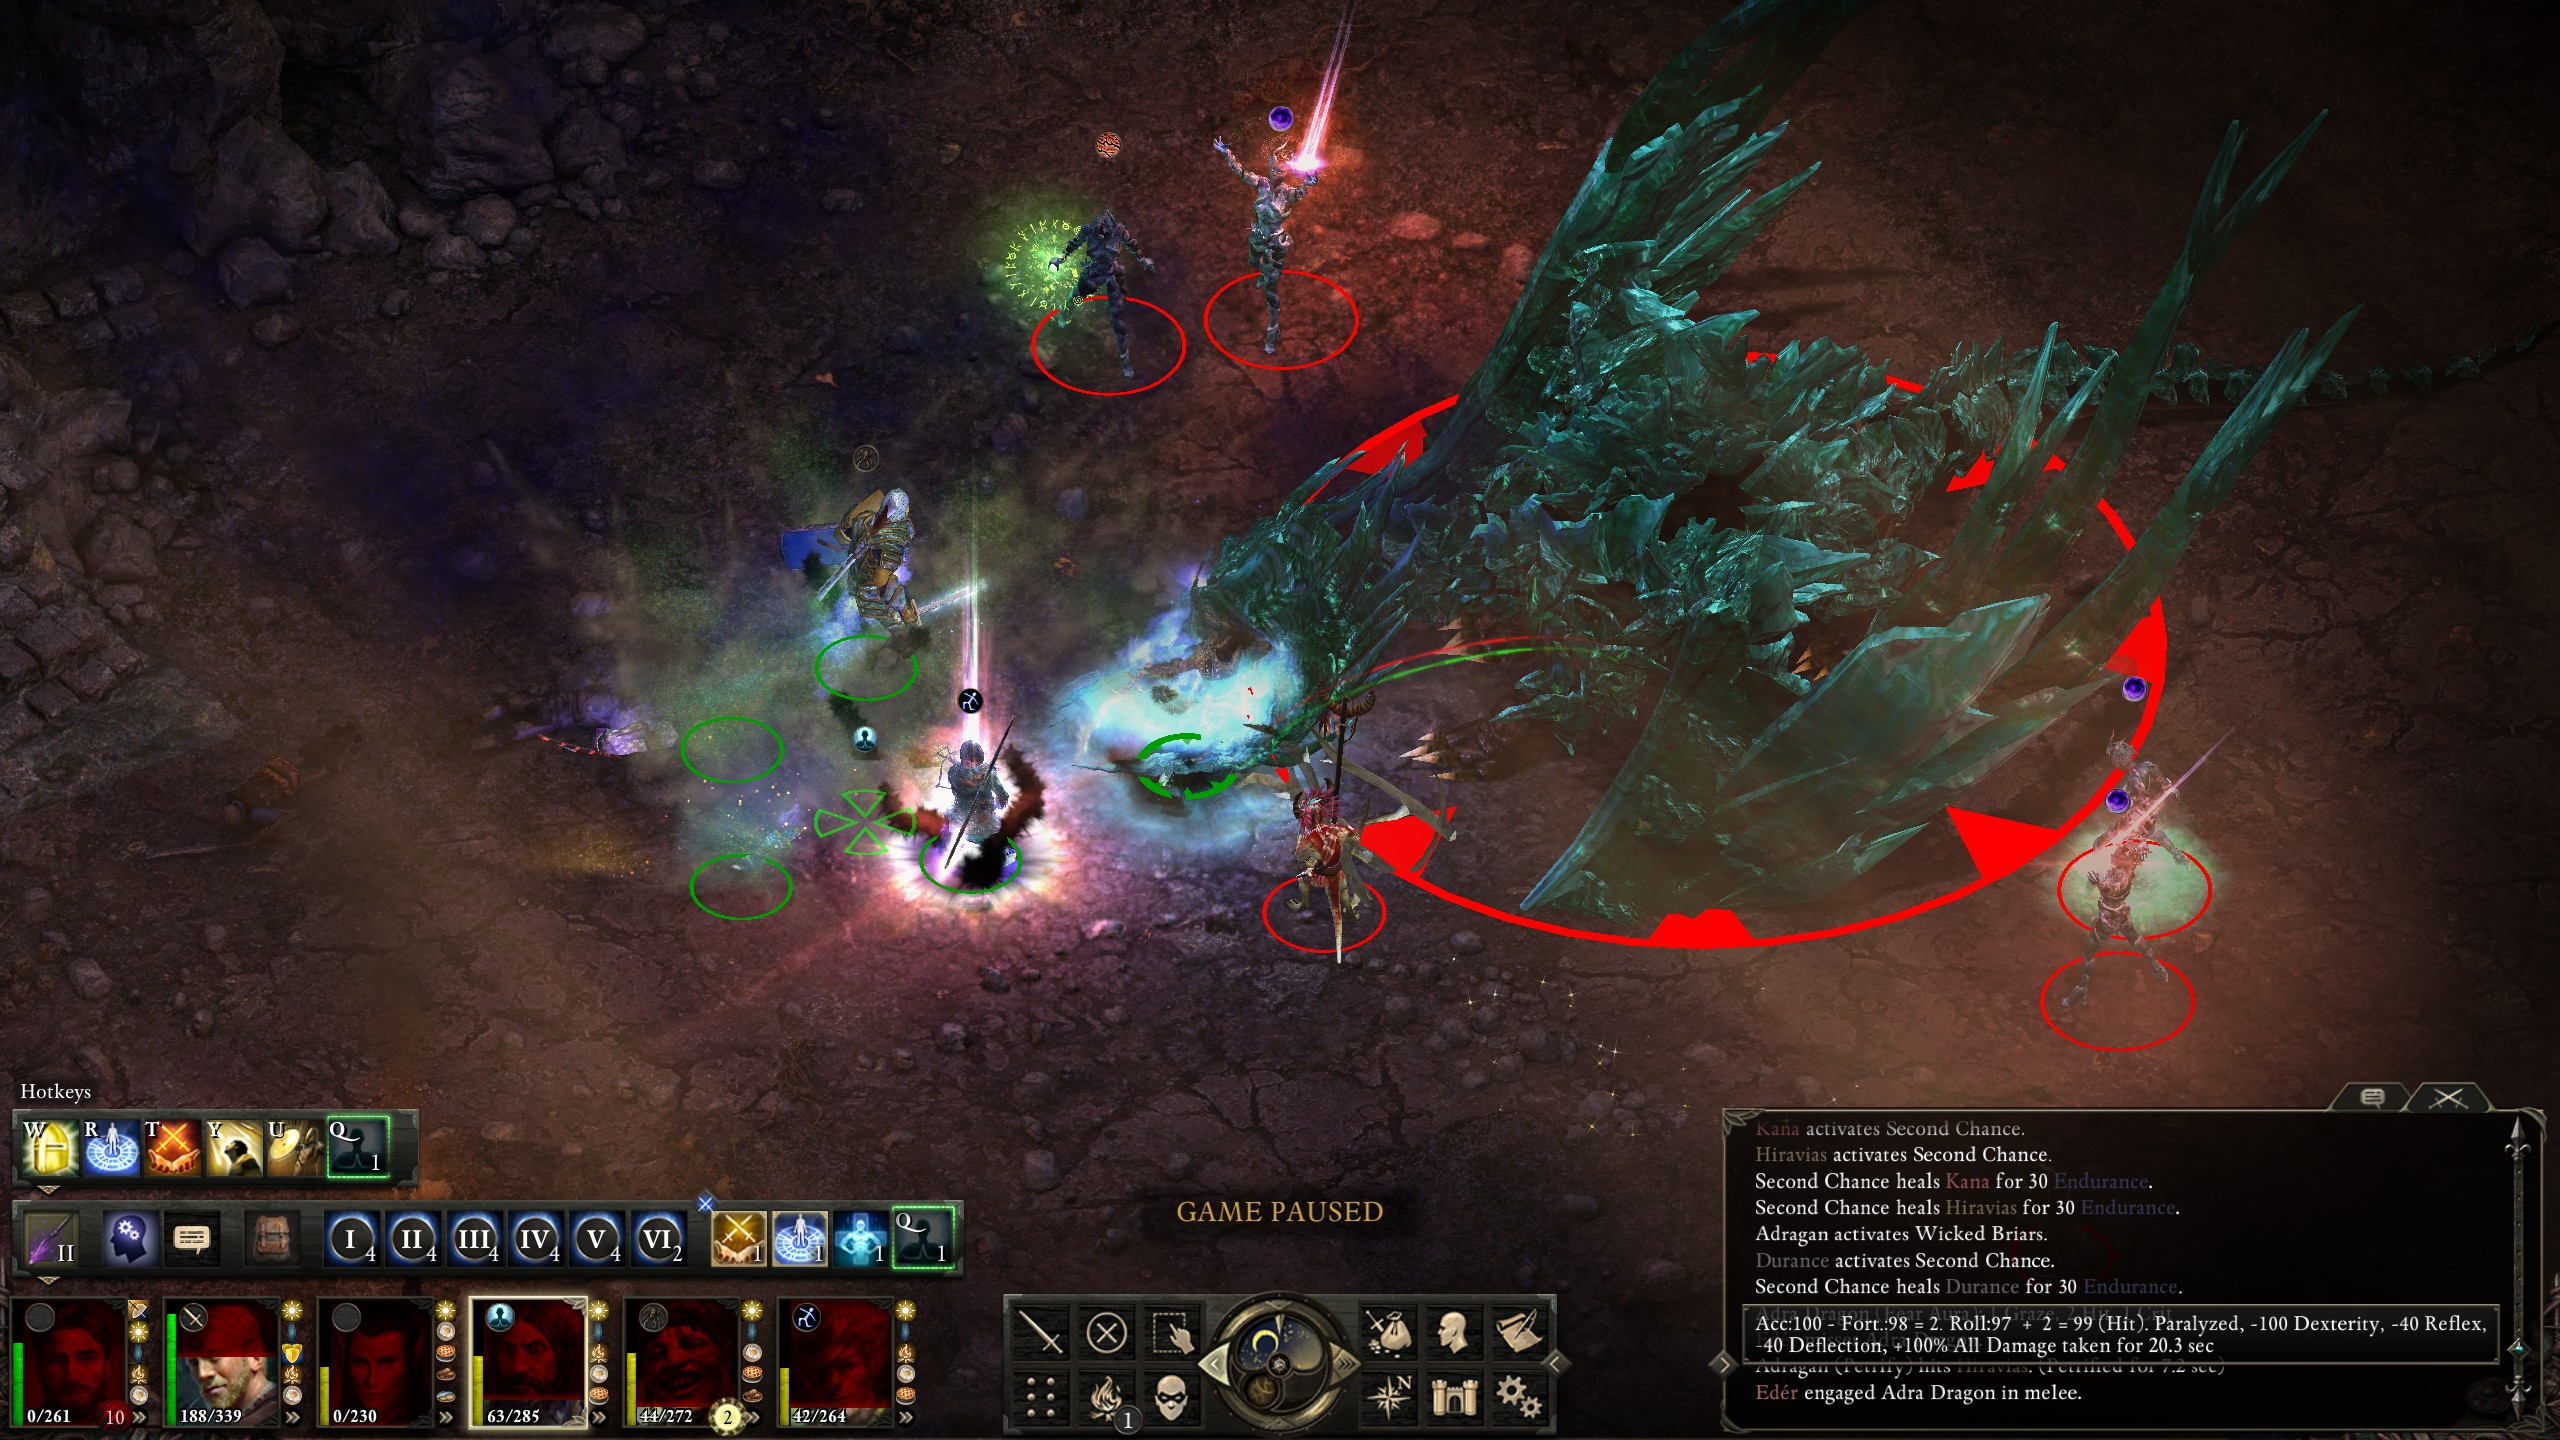
\includegraphics[scale=0.33]{files/blog/2019_03_17_pillars_of_eternity_path_of_the_damned_act_iv/2019_03_17_dragon1_03.jpg}
\end{figure}

Then one of the adragans landed a petrification on Hiravas.  At this point I almost rage-quit, but I decided to stick it out anyways in case I'd learn something.  Luckily, Hiravas managed to recover rapidly from the petrify (perhaps he had managed to drink the potion, or perhaps he bugged out of it), and I started having Durance revive Aloth and my monk.

\begin{figure}
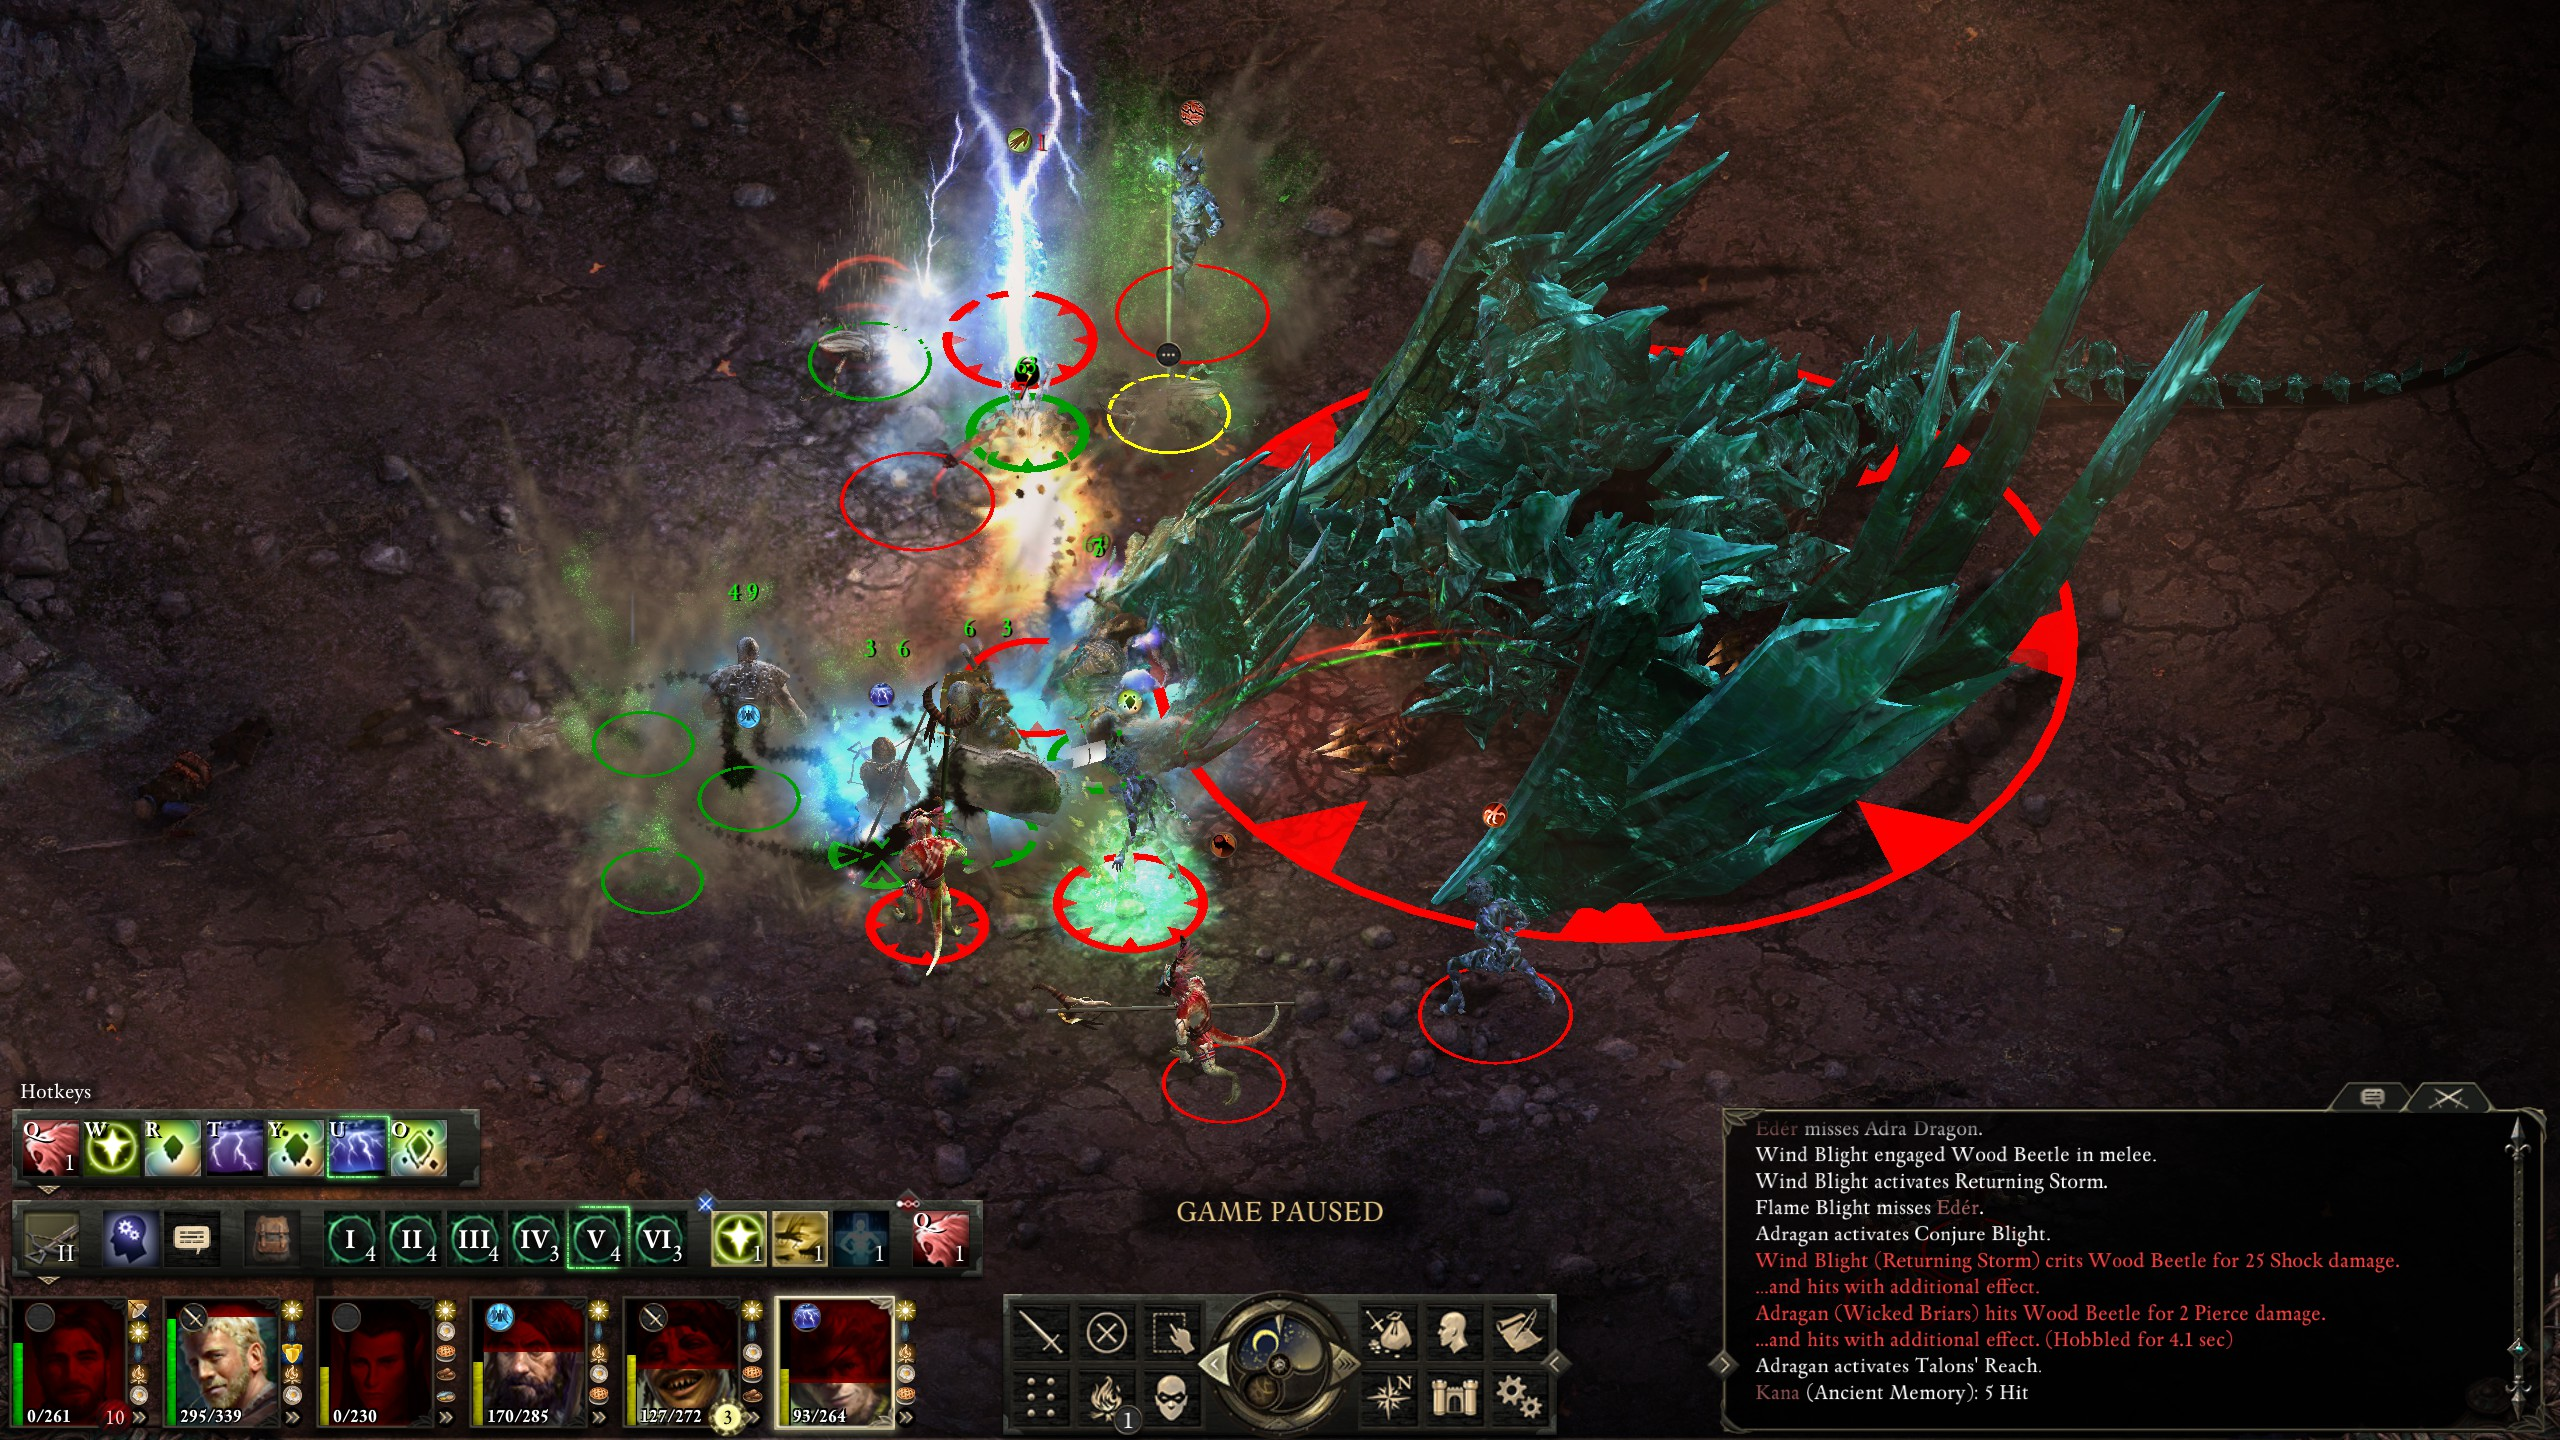
\includegraphics[scale=0.33]{files/blog/2019_03_17_pillars_of_eternity_path_of_the_damned_act_iv/2019_03_17_dragon1_04.jpg}
\end{figure}

With Aloth up I then combo'd "Call to Slumber" with a "Minoletta's Precisely Piercing Burst", and thus annihilated the adds far quicker than expected.  I also had Durance begin casting "Barring Death's Door" on those close to death.

\begin{figure}
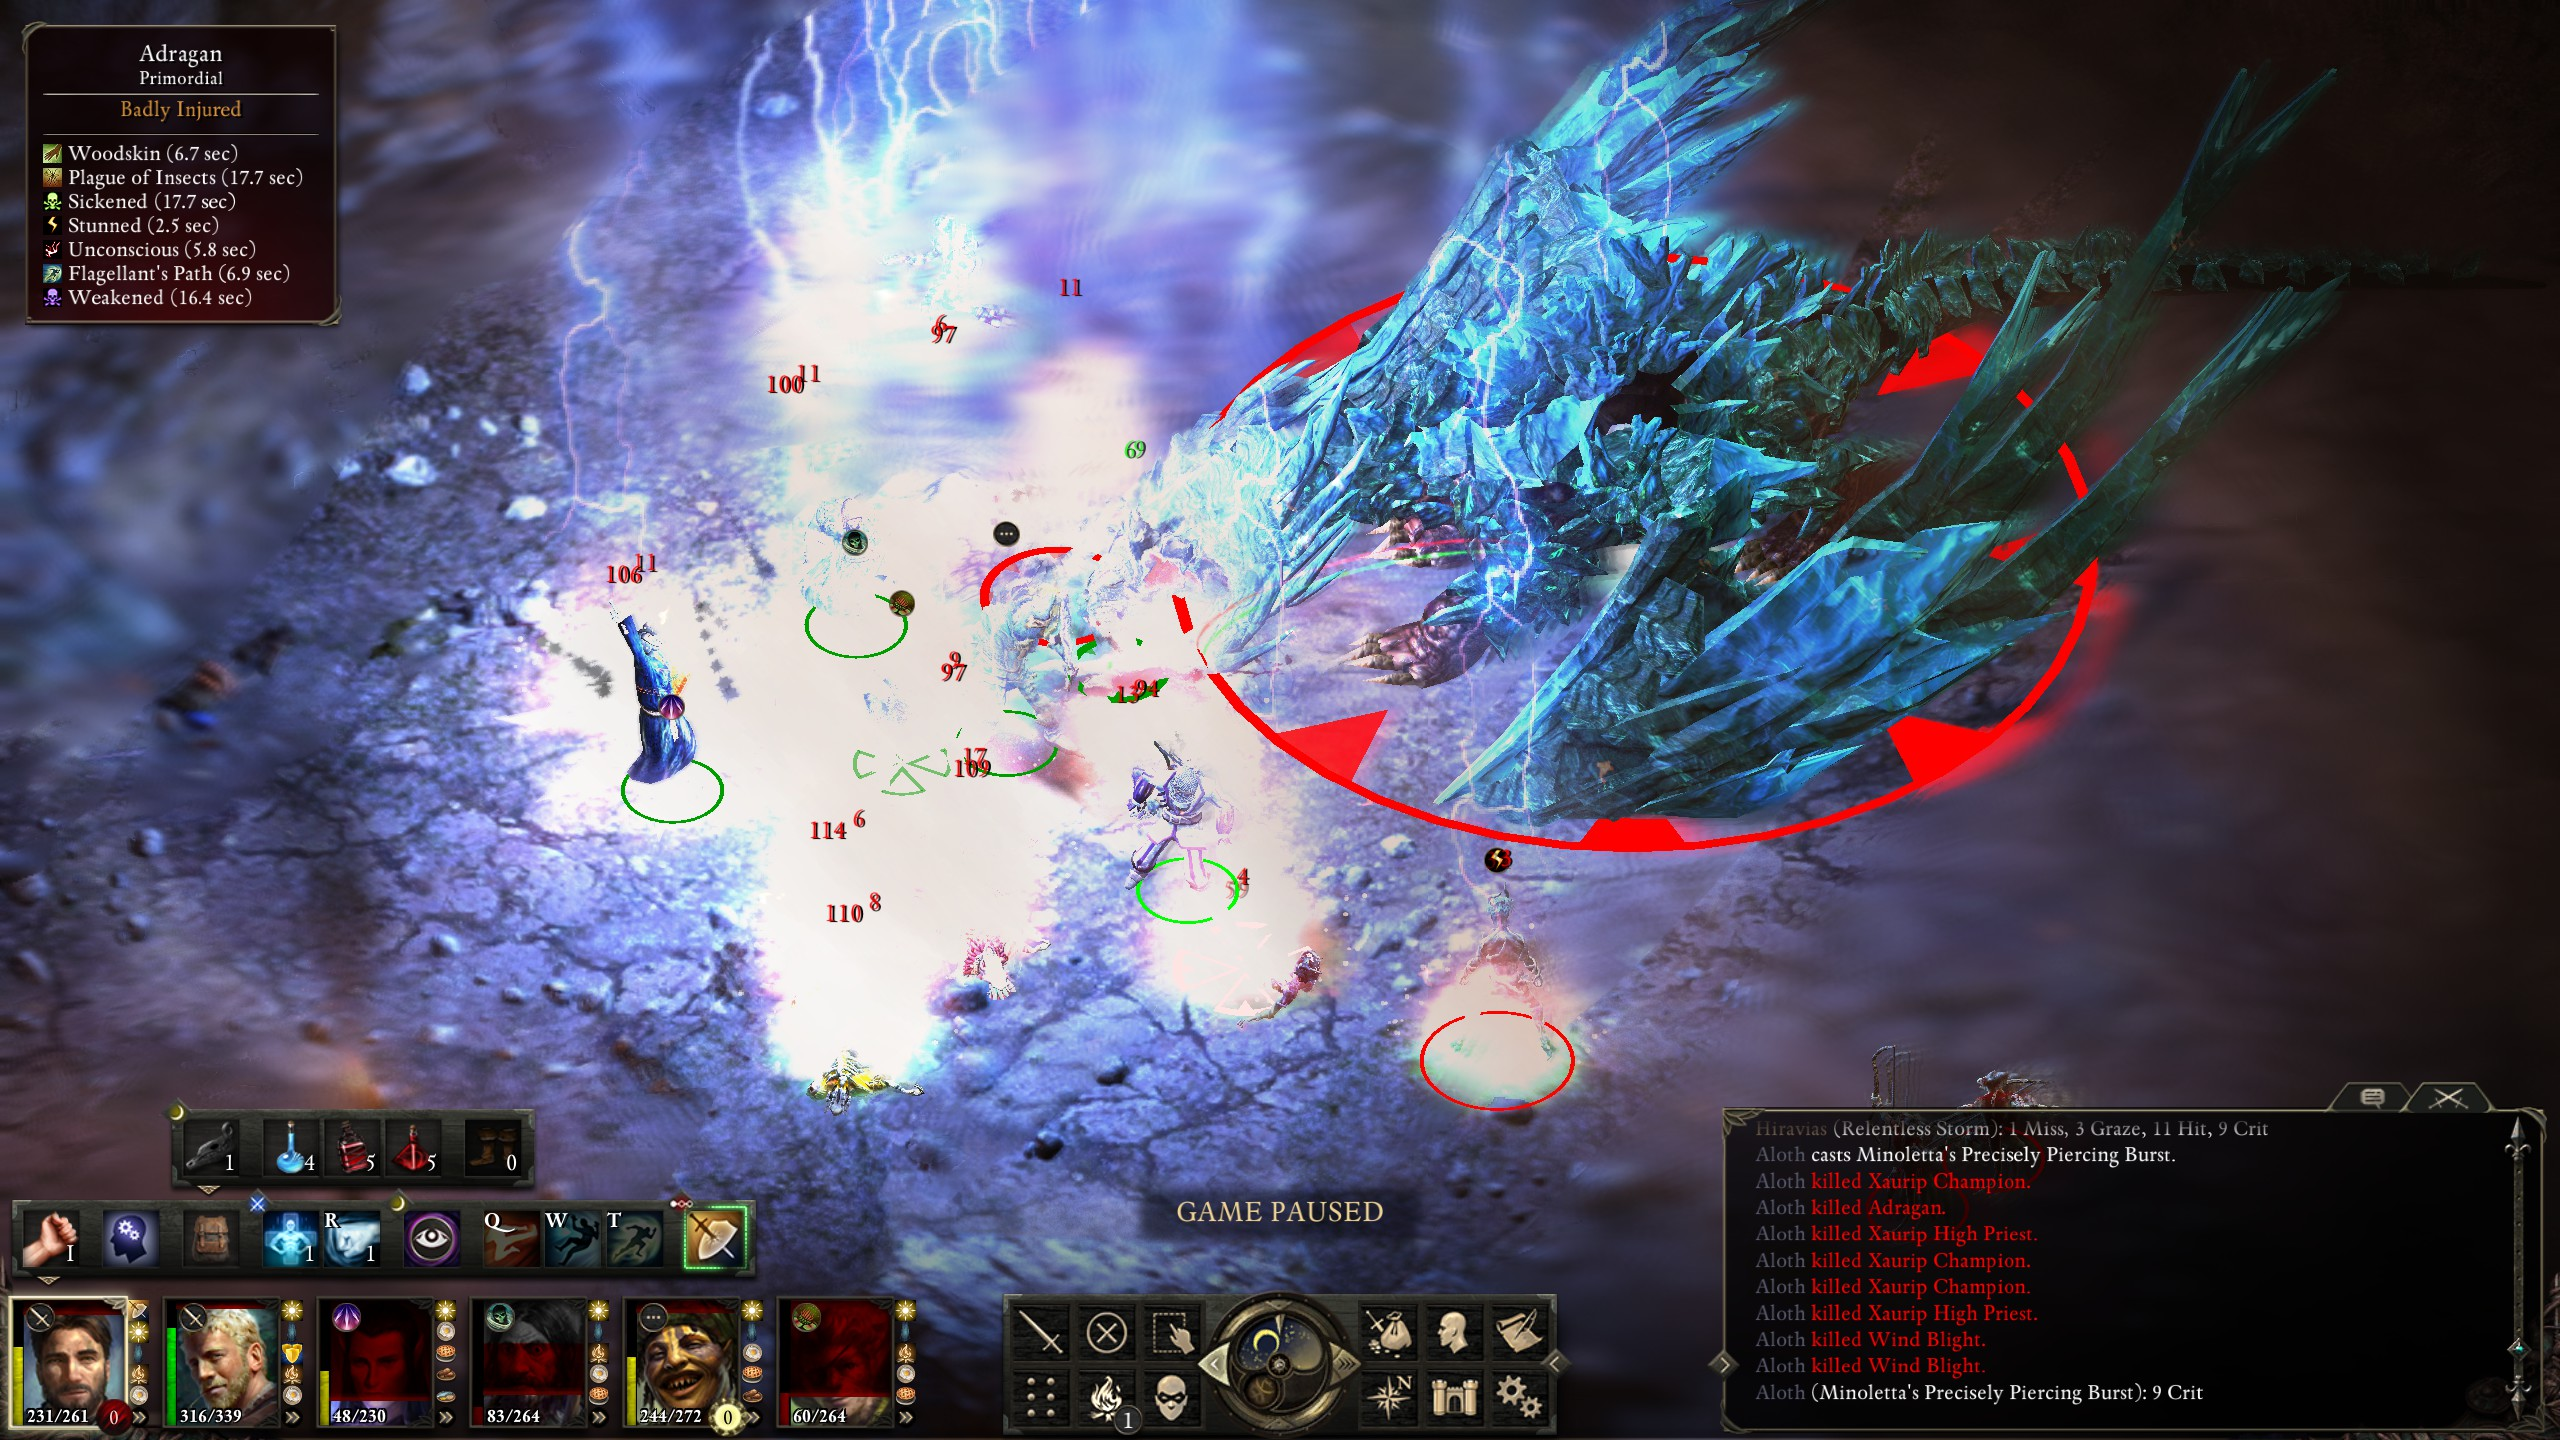
\includegraphics[scale=0.33]{files/blog/2019_03_17_pillars_of_eternity_path_of_the_damned_act_iv/2019_03_17_dragon1_05.jpg}
\end{figure}

Perhaps, I thought, I would make it though.  The dragon, of course, decided to cut straight into my hopes.

\begin{figure}
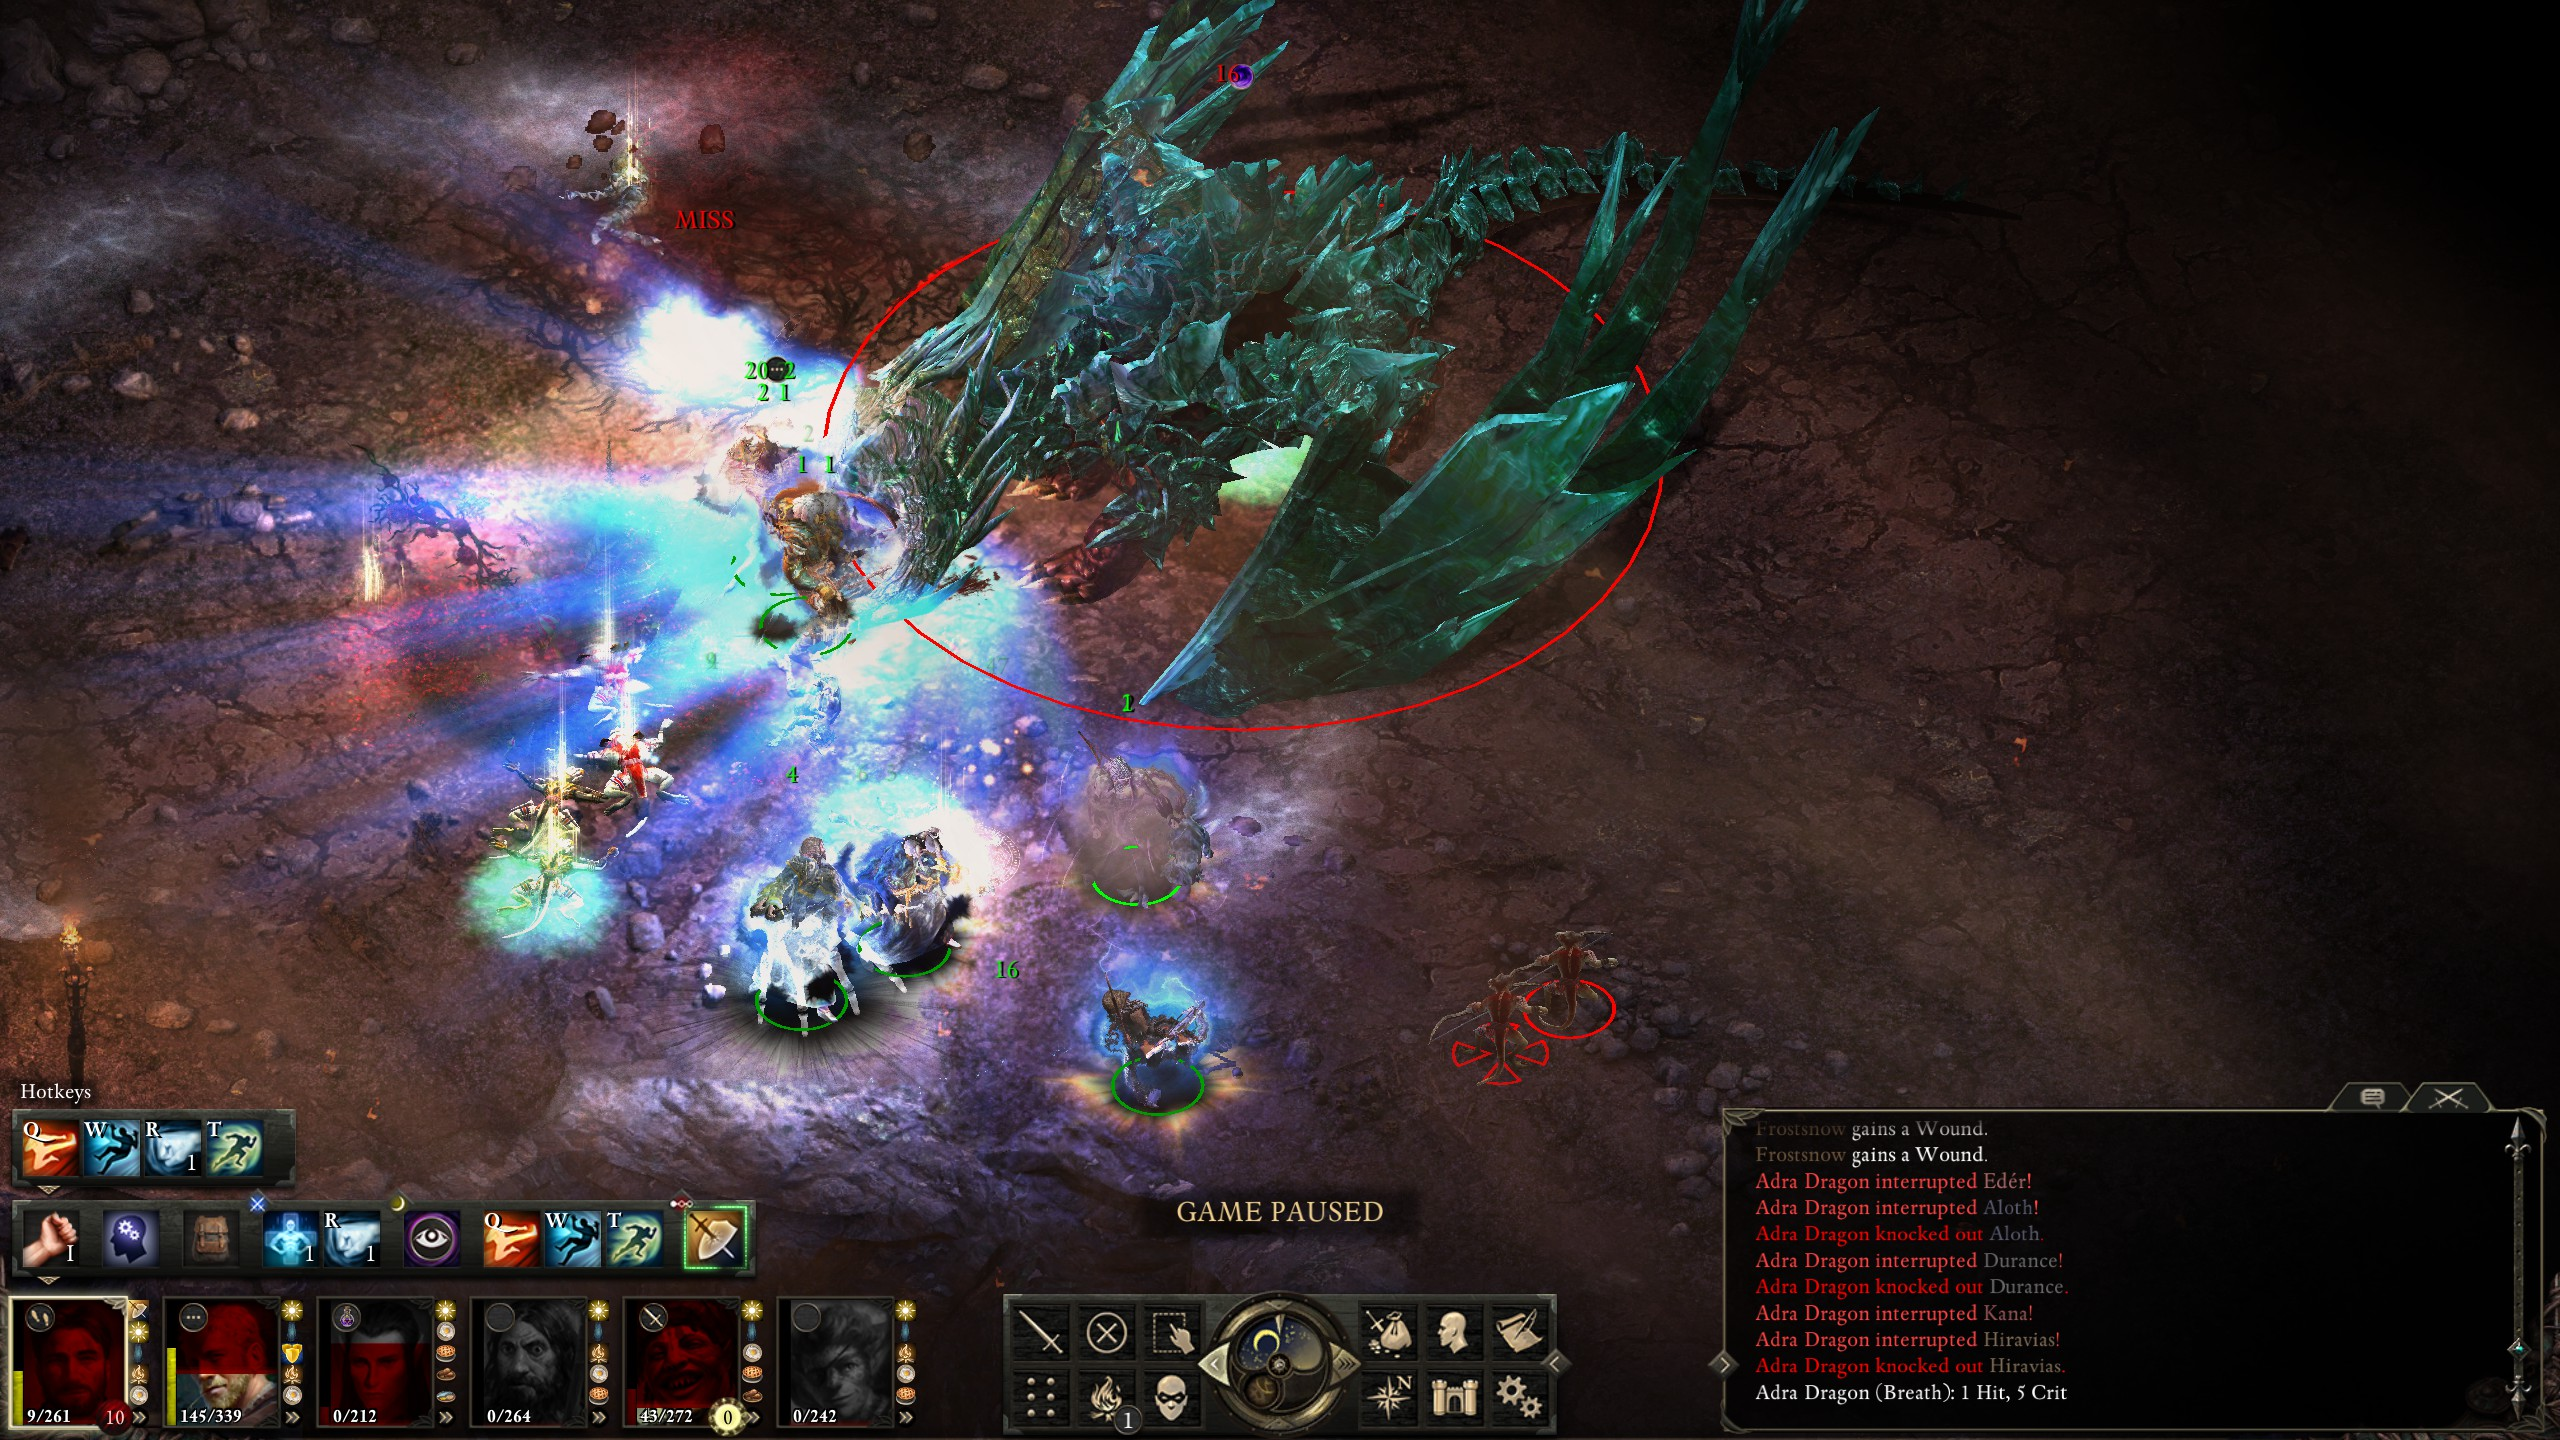
\includegraphics[scale=0.33]{files/blog/2019_03_17_pillars_of_eternity_path_of_the_damned_act_iv/2019_03_17_dragon1_06.jpg}
\end{figure}

Good thing I'd cast "Barring Death's Door" on those two.  After a while I managed to revive Aloth with Kana and have Aloth use "Infuse With Vital Essence" in order gain enough health to survive another knockout, then moved him and my monk into the southeast position as Kana was currently engaged by the dragon.

\begin{figure}
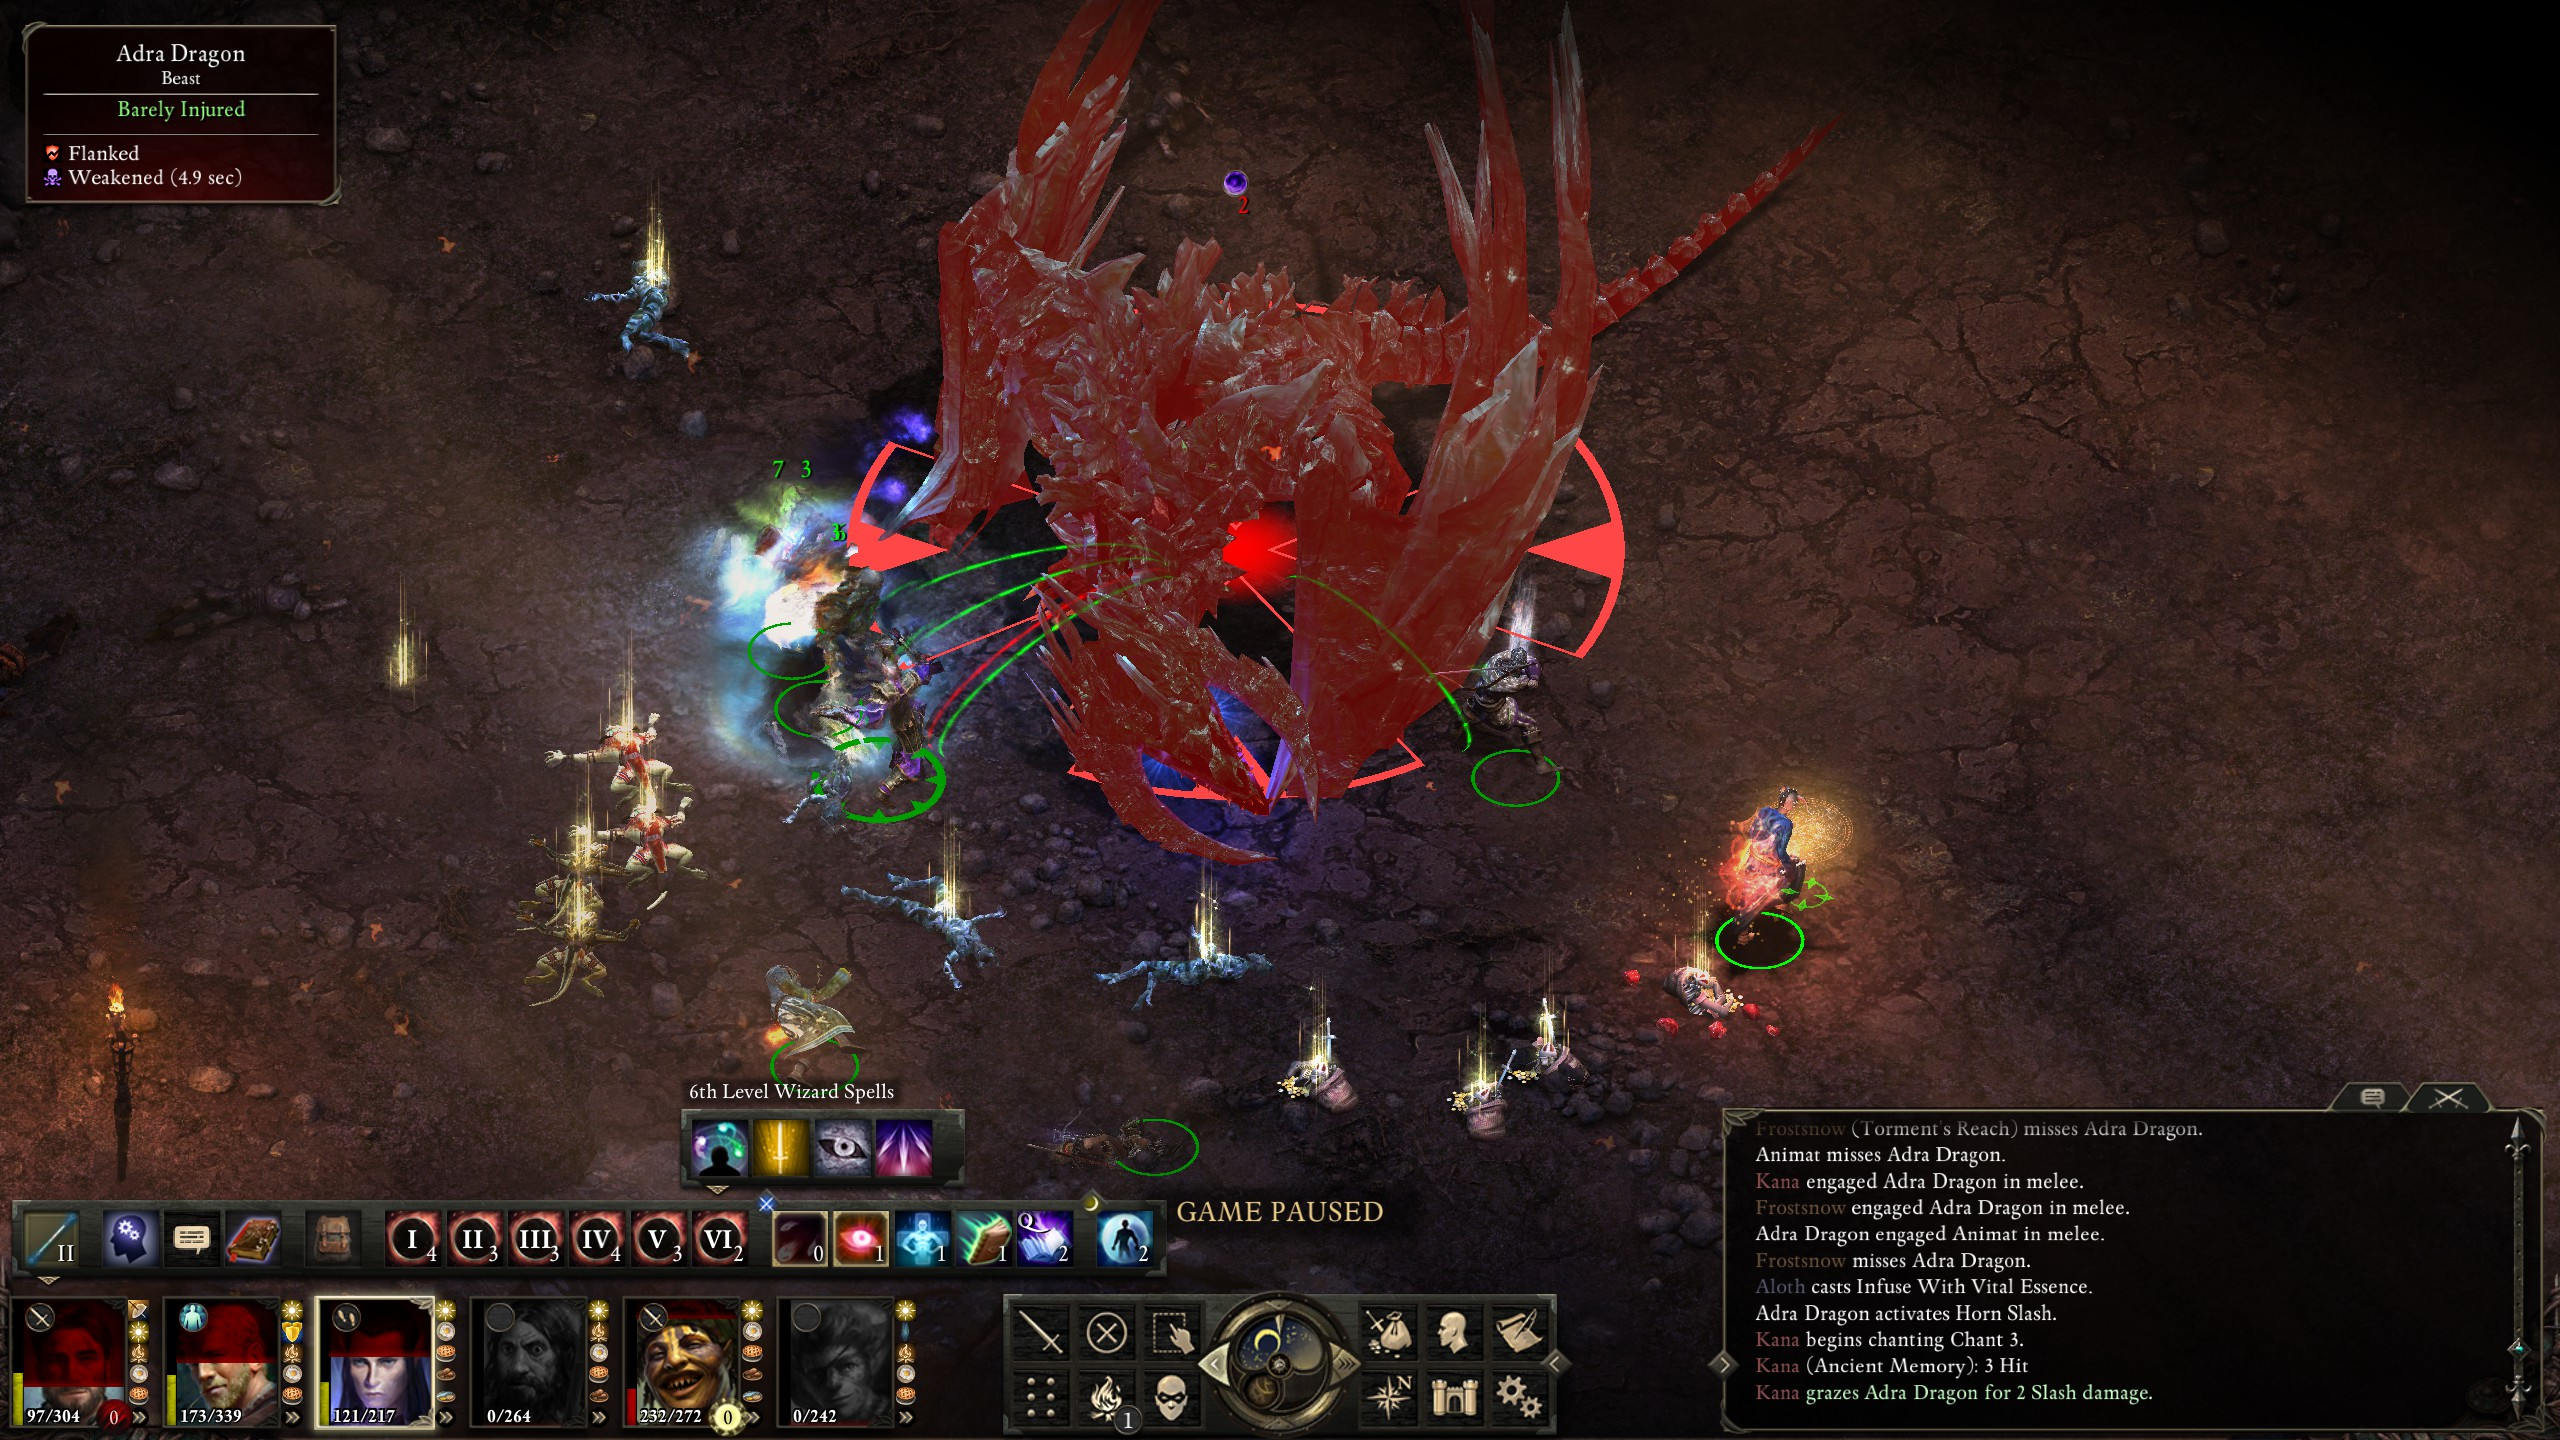
\includegraphics[scale=0.33]{files/blog/2019_03_17_pillars_of_eternity_path_of_the_damned_act_iv/2019_03_17_dragon1_07.jpg}
\end{figure}

The dragon did not appreciate this.

\begin{figure}
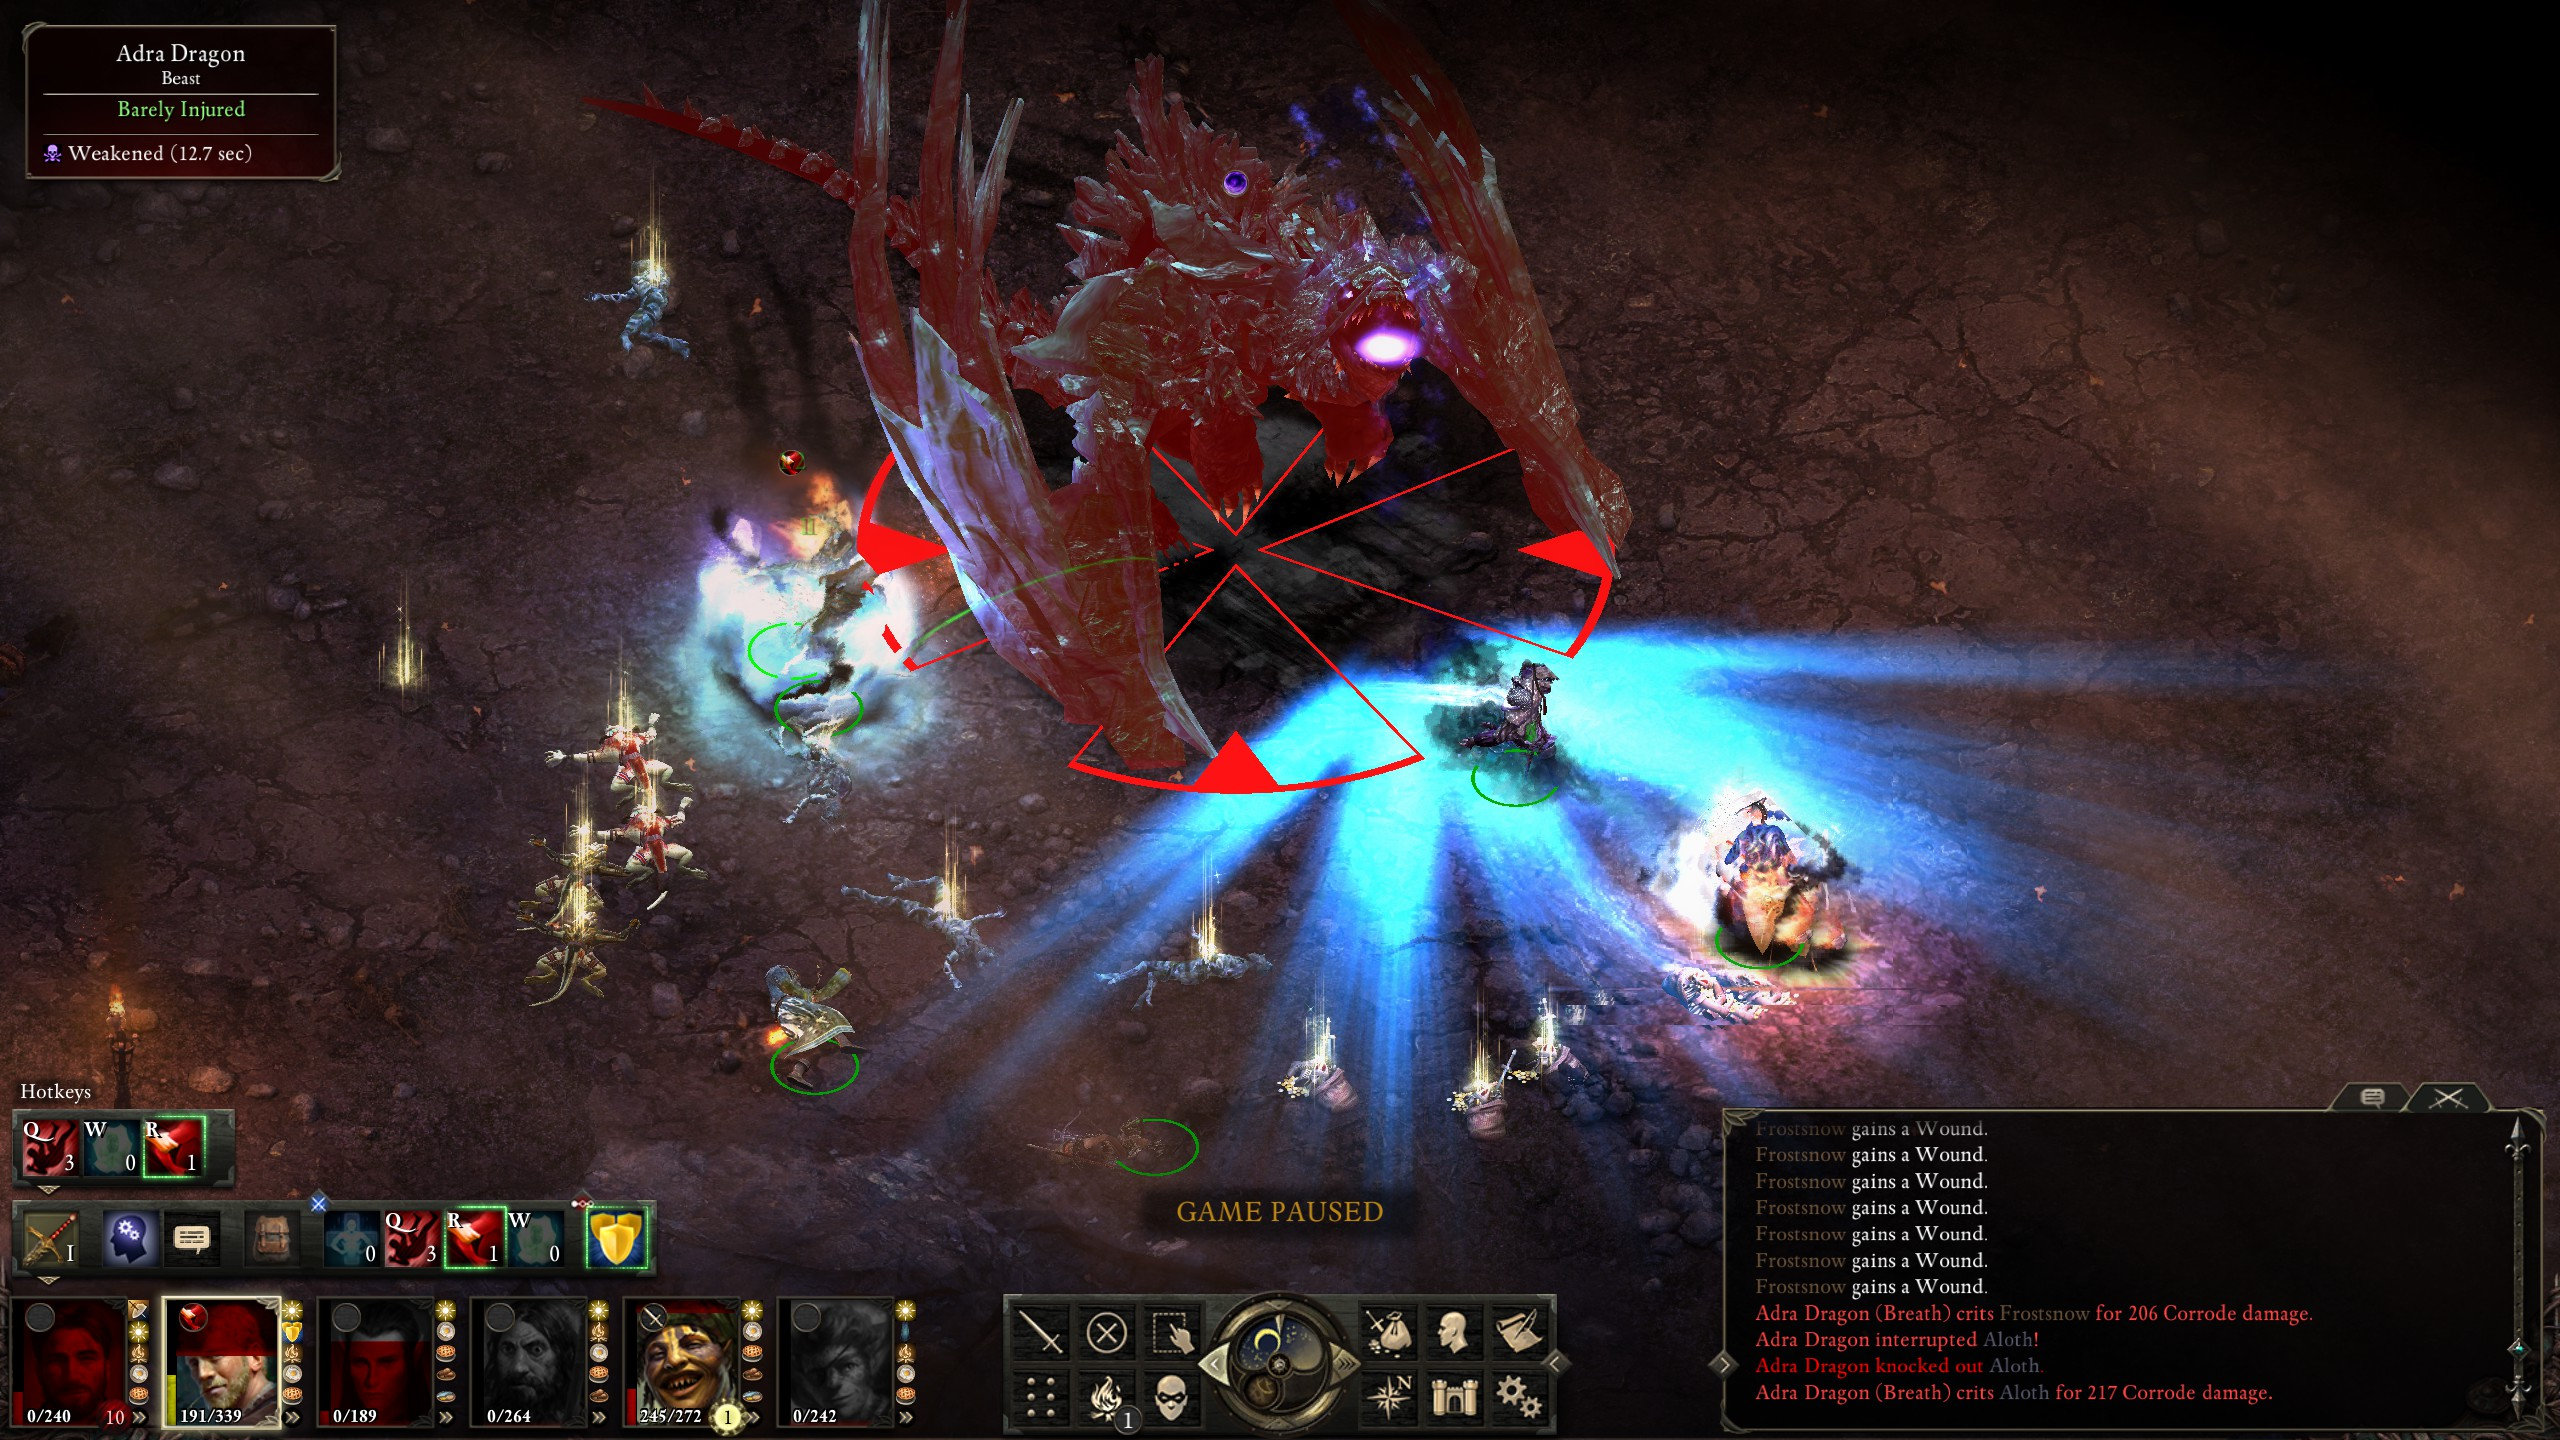
\includegraphics[scale=0.33]{files/blog/2019_03_17_pillars_of_eternity_path_of_the_damned_act_iv/2019_03_17_dragon1_08.jpg}
\end{figure}

Again, I was able to move Kana into a position to revive Aloth and also my monk while moving into the southeast corner.  I then moved Aloth to the southwest corner and proceeded to cast spells with a series of rock-bottom rolls while the dragon decided to engage my monk rather than Kana.

\begin{figure}
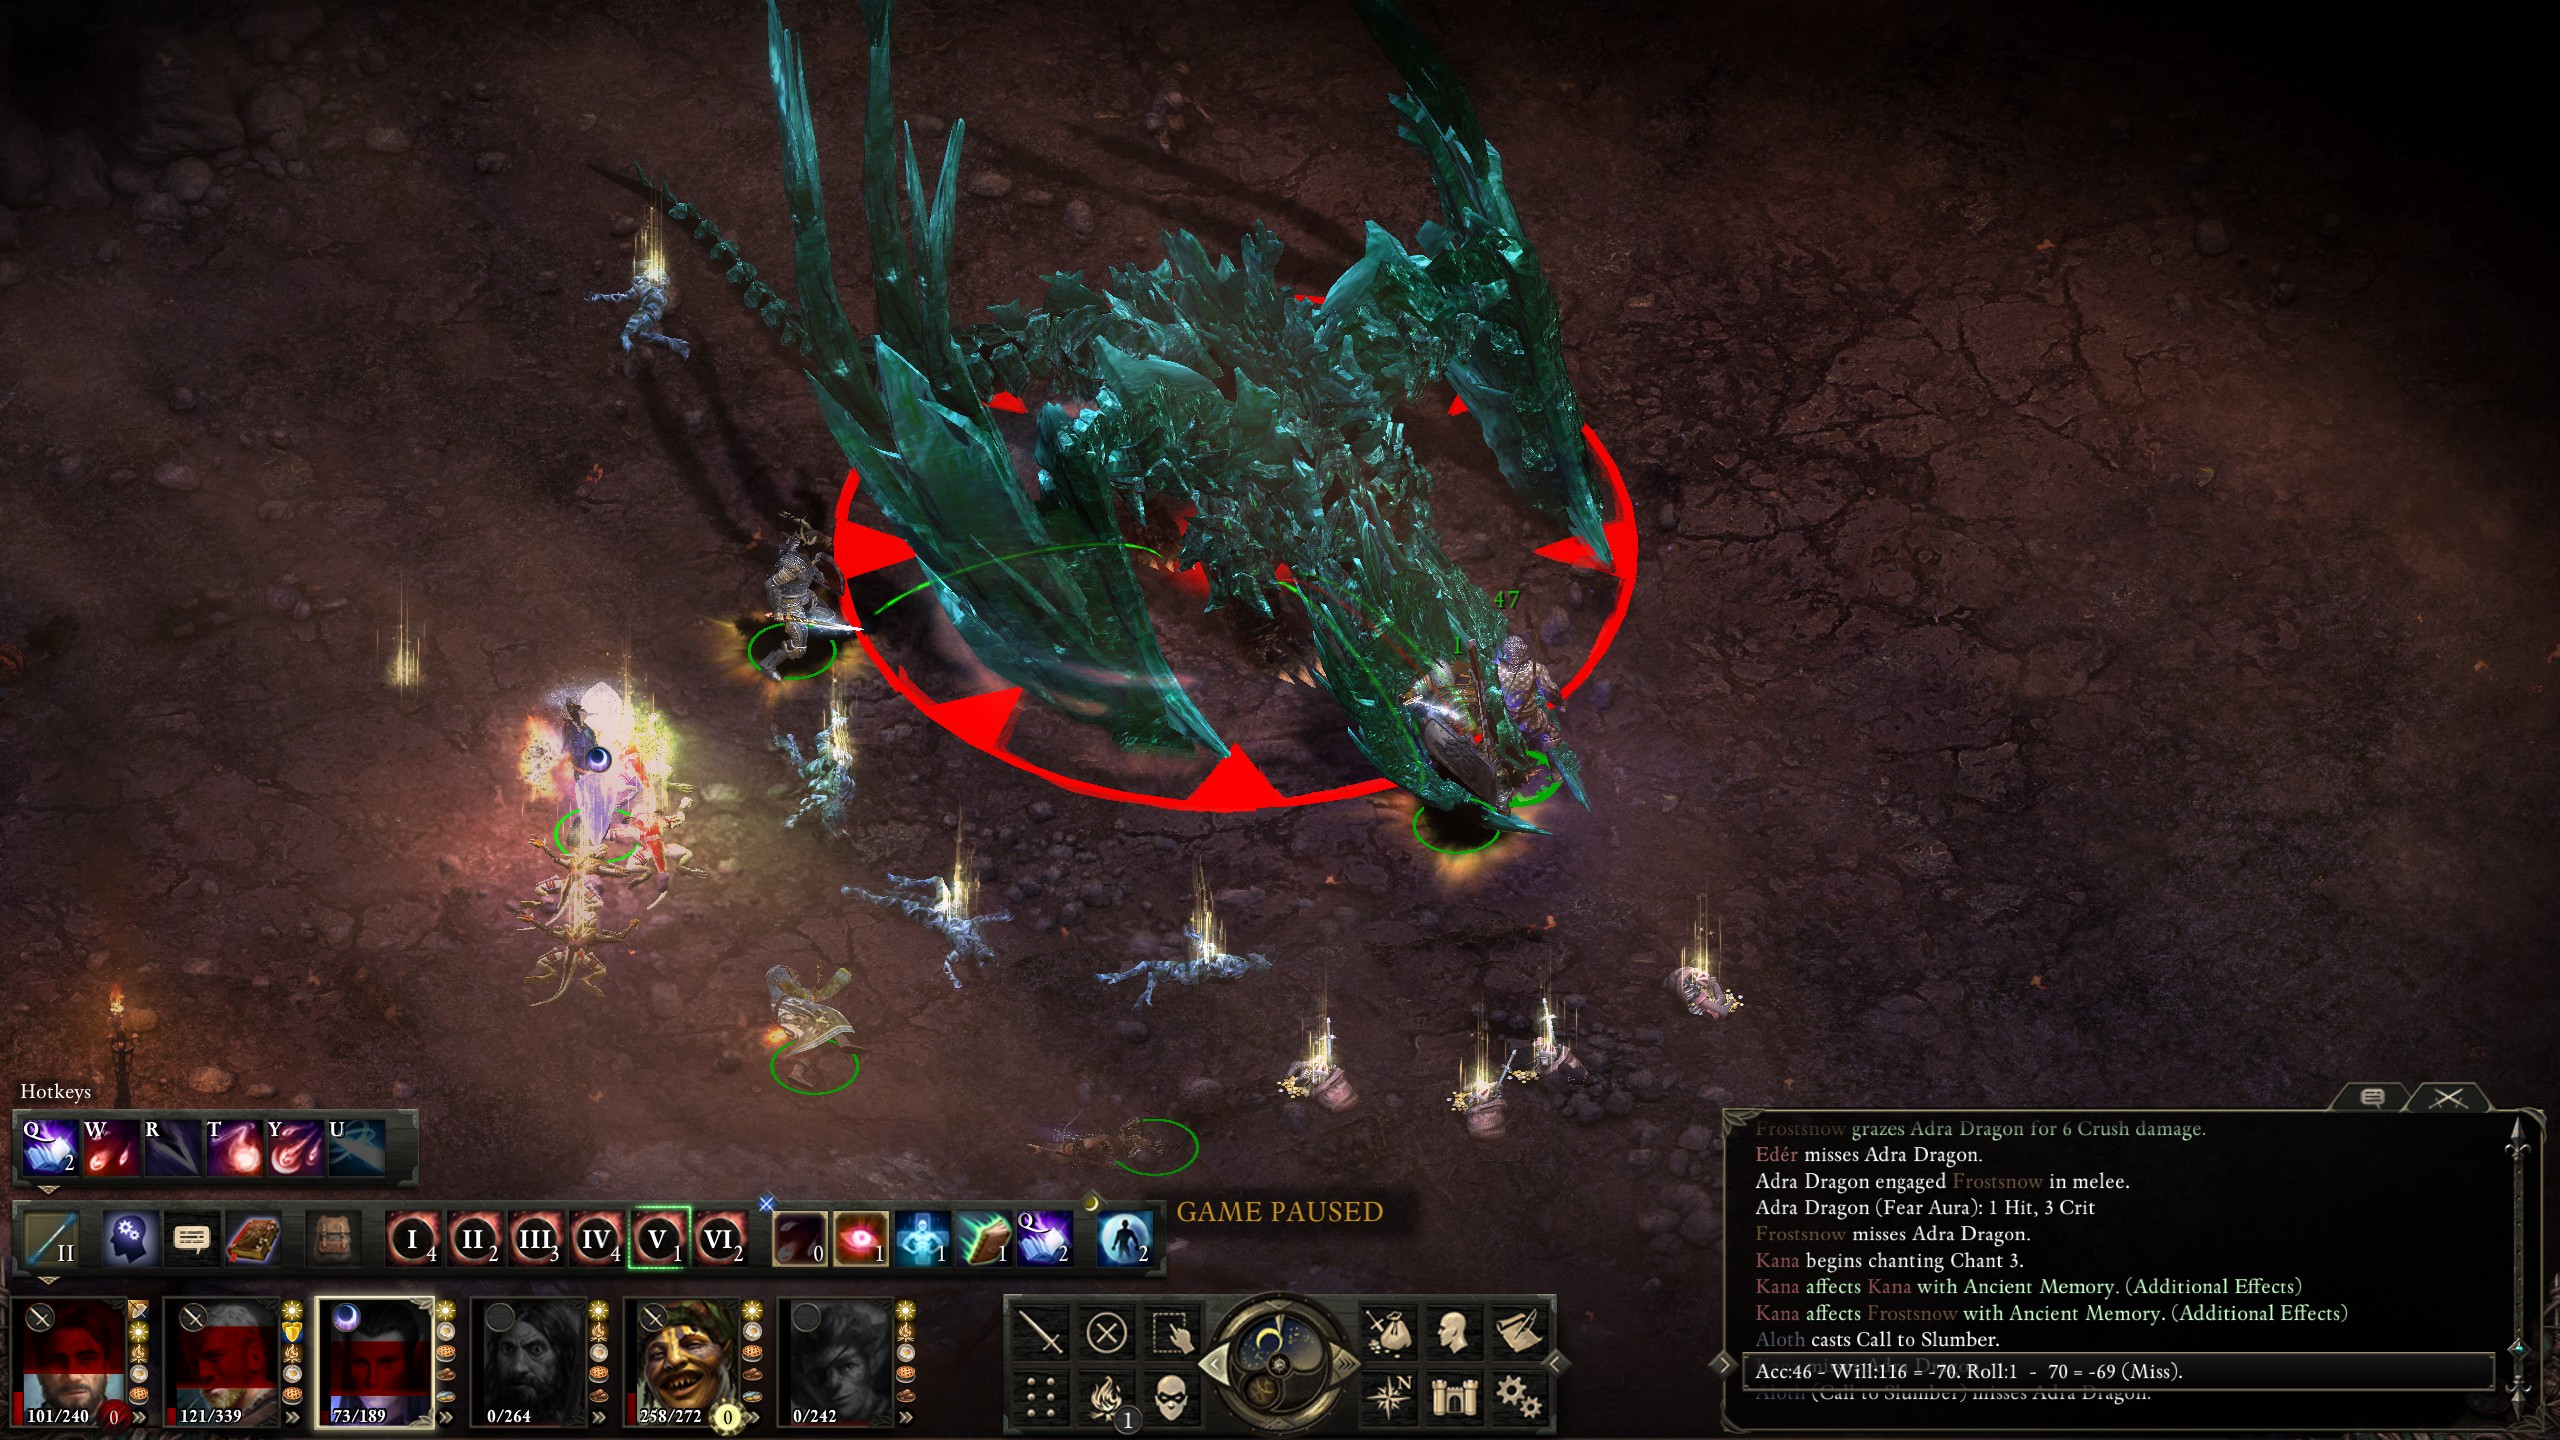
\includegraphics[scale=0.33]{files/blog/2019_03_17_pillars_of_eternity_path_of_the_damned_act_iv/2019_03_17_dragon1_09.jpg}
\end{figure}

After knocking my Monk out it then proceeded to \emph{kill} Eder and Aloth with another Breath attack.

\begin{figure}
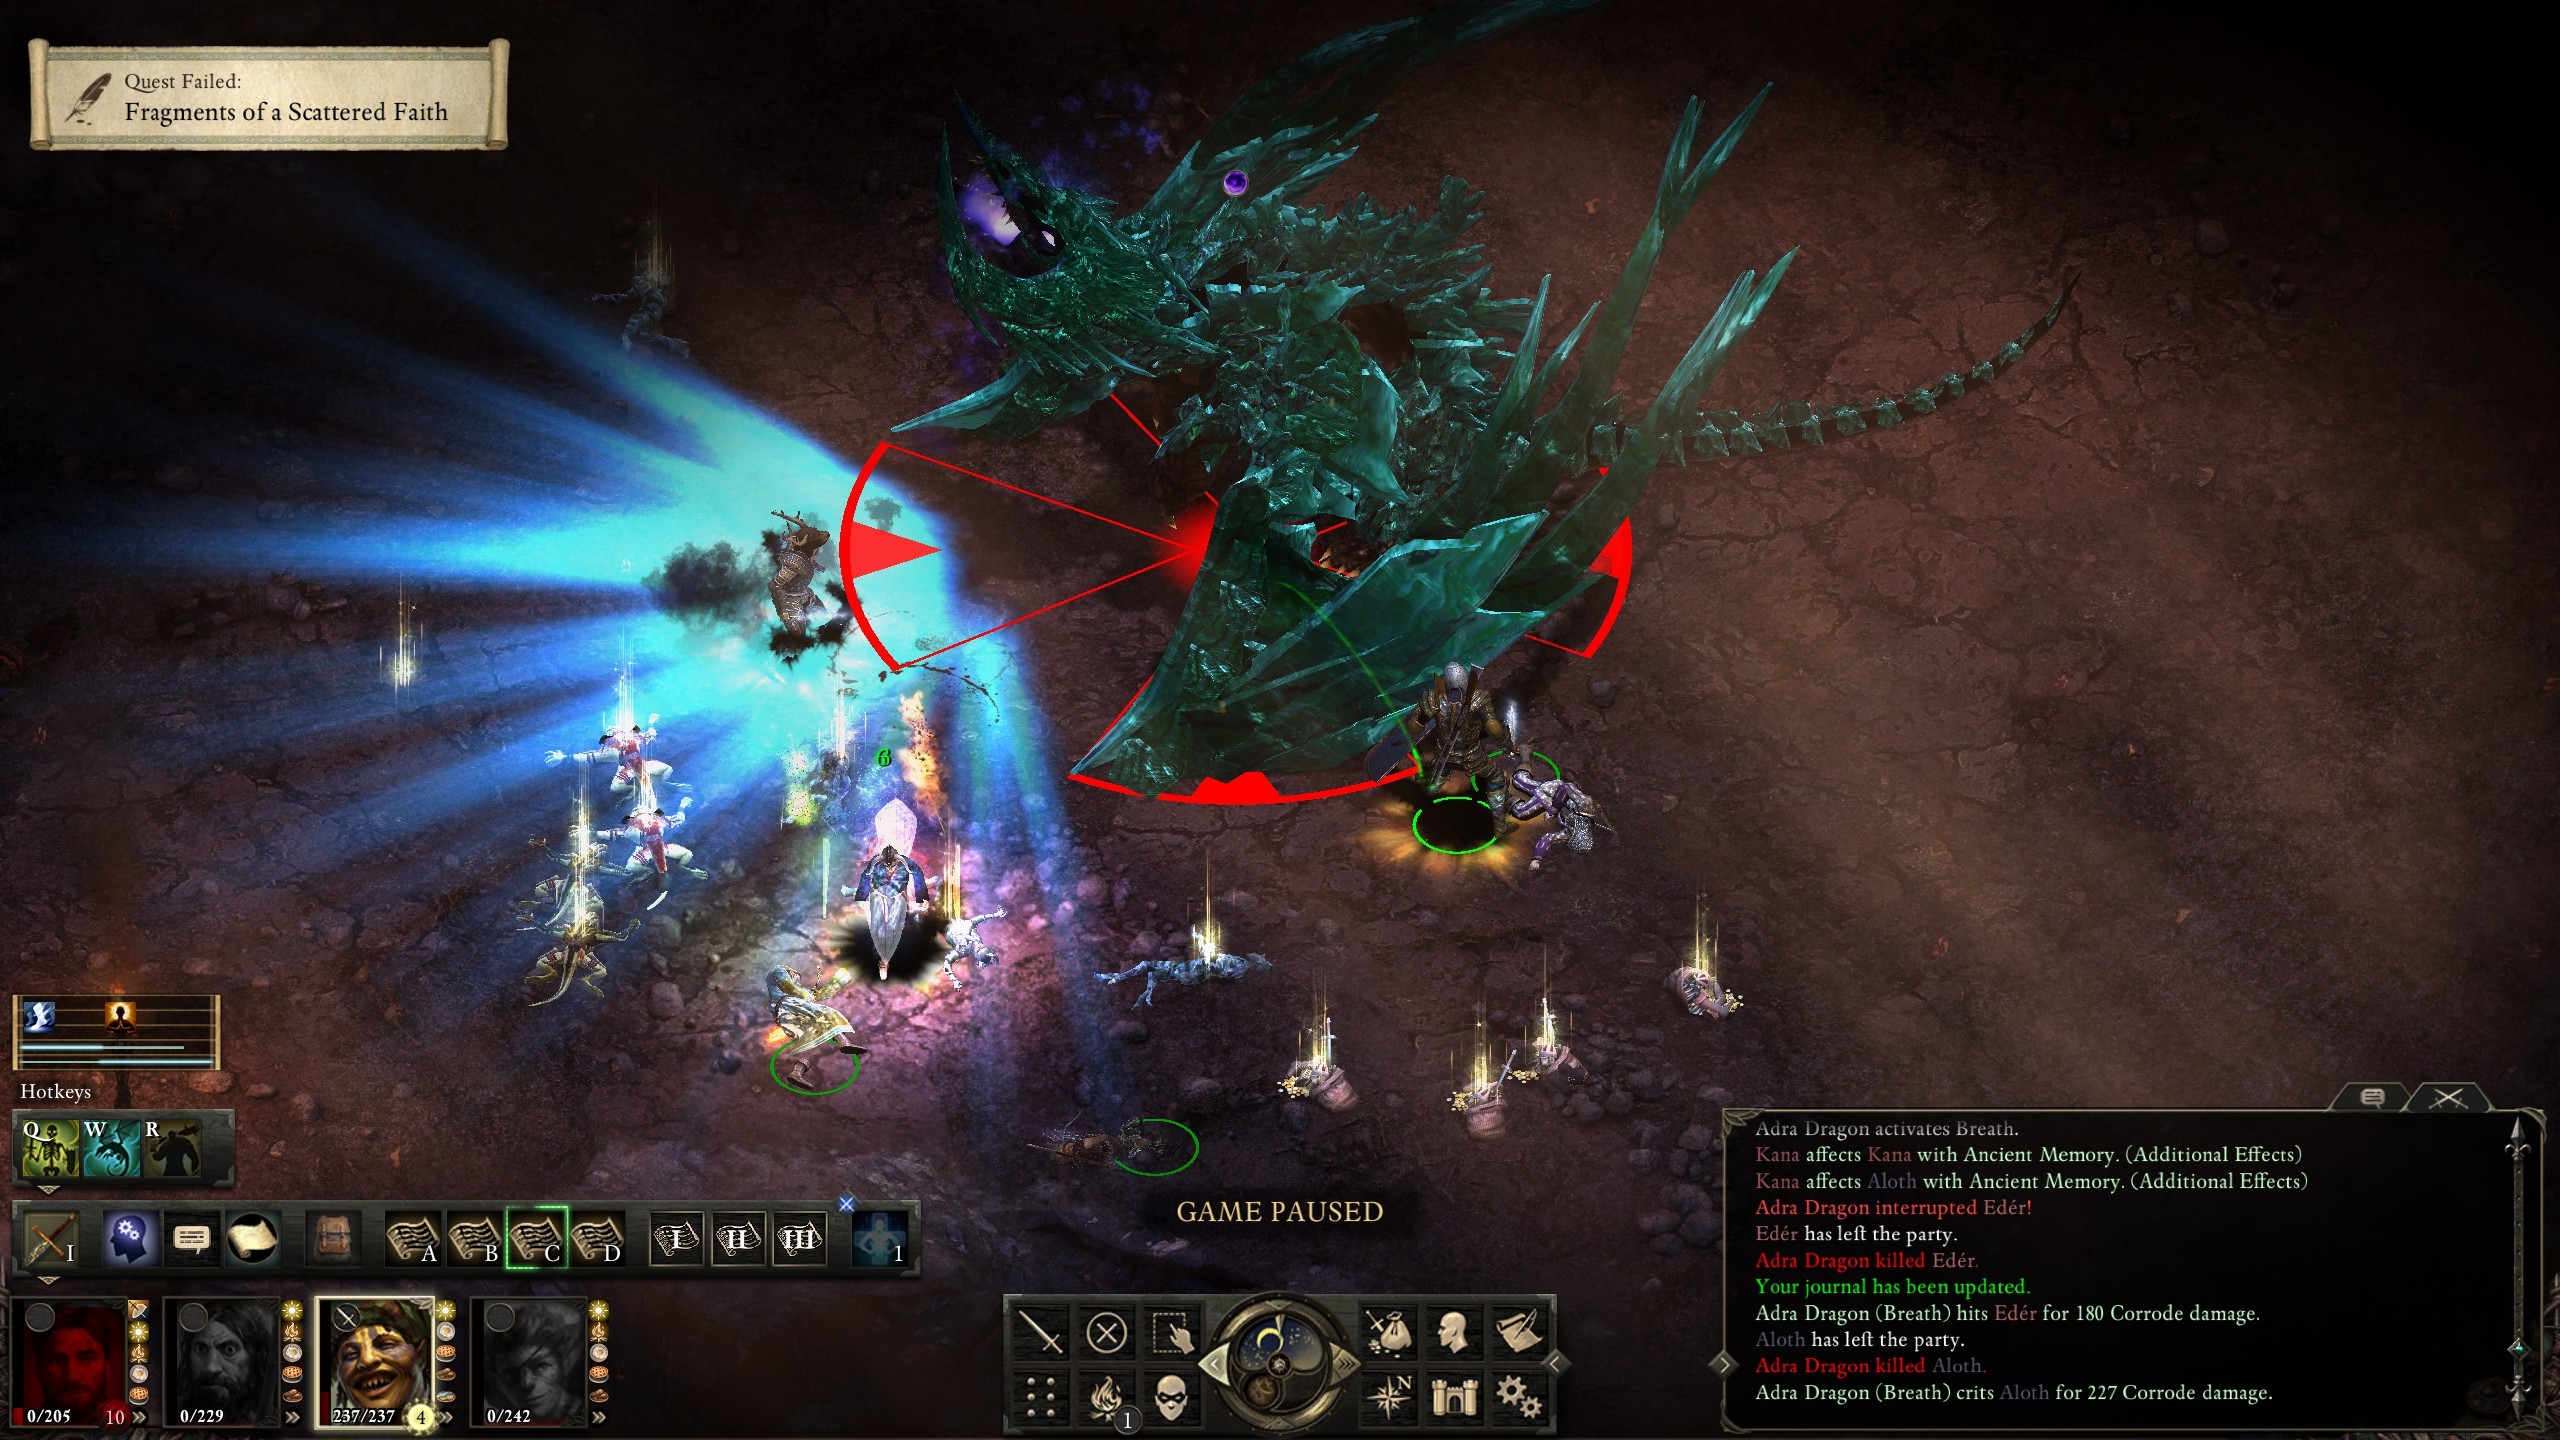
\includegraphics[scale=0.33]{files/blog/2019_03_17_pillars_of_eternity_path_of_the_damned_act_iv/2019_03_17_dragon1_10.jpg}
\end{figure}

Kana then lived long enough to revive my monk before also dying.

\begin{figure}
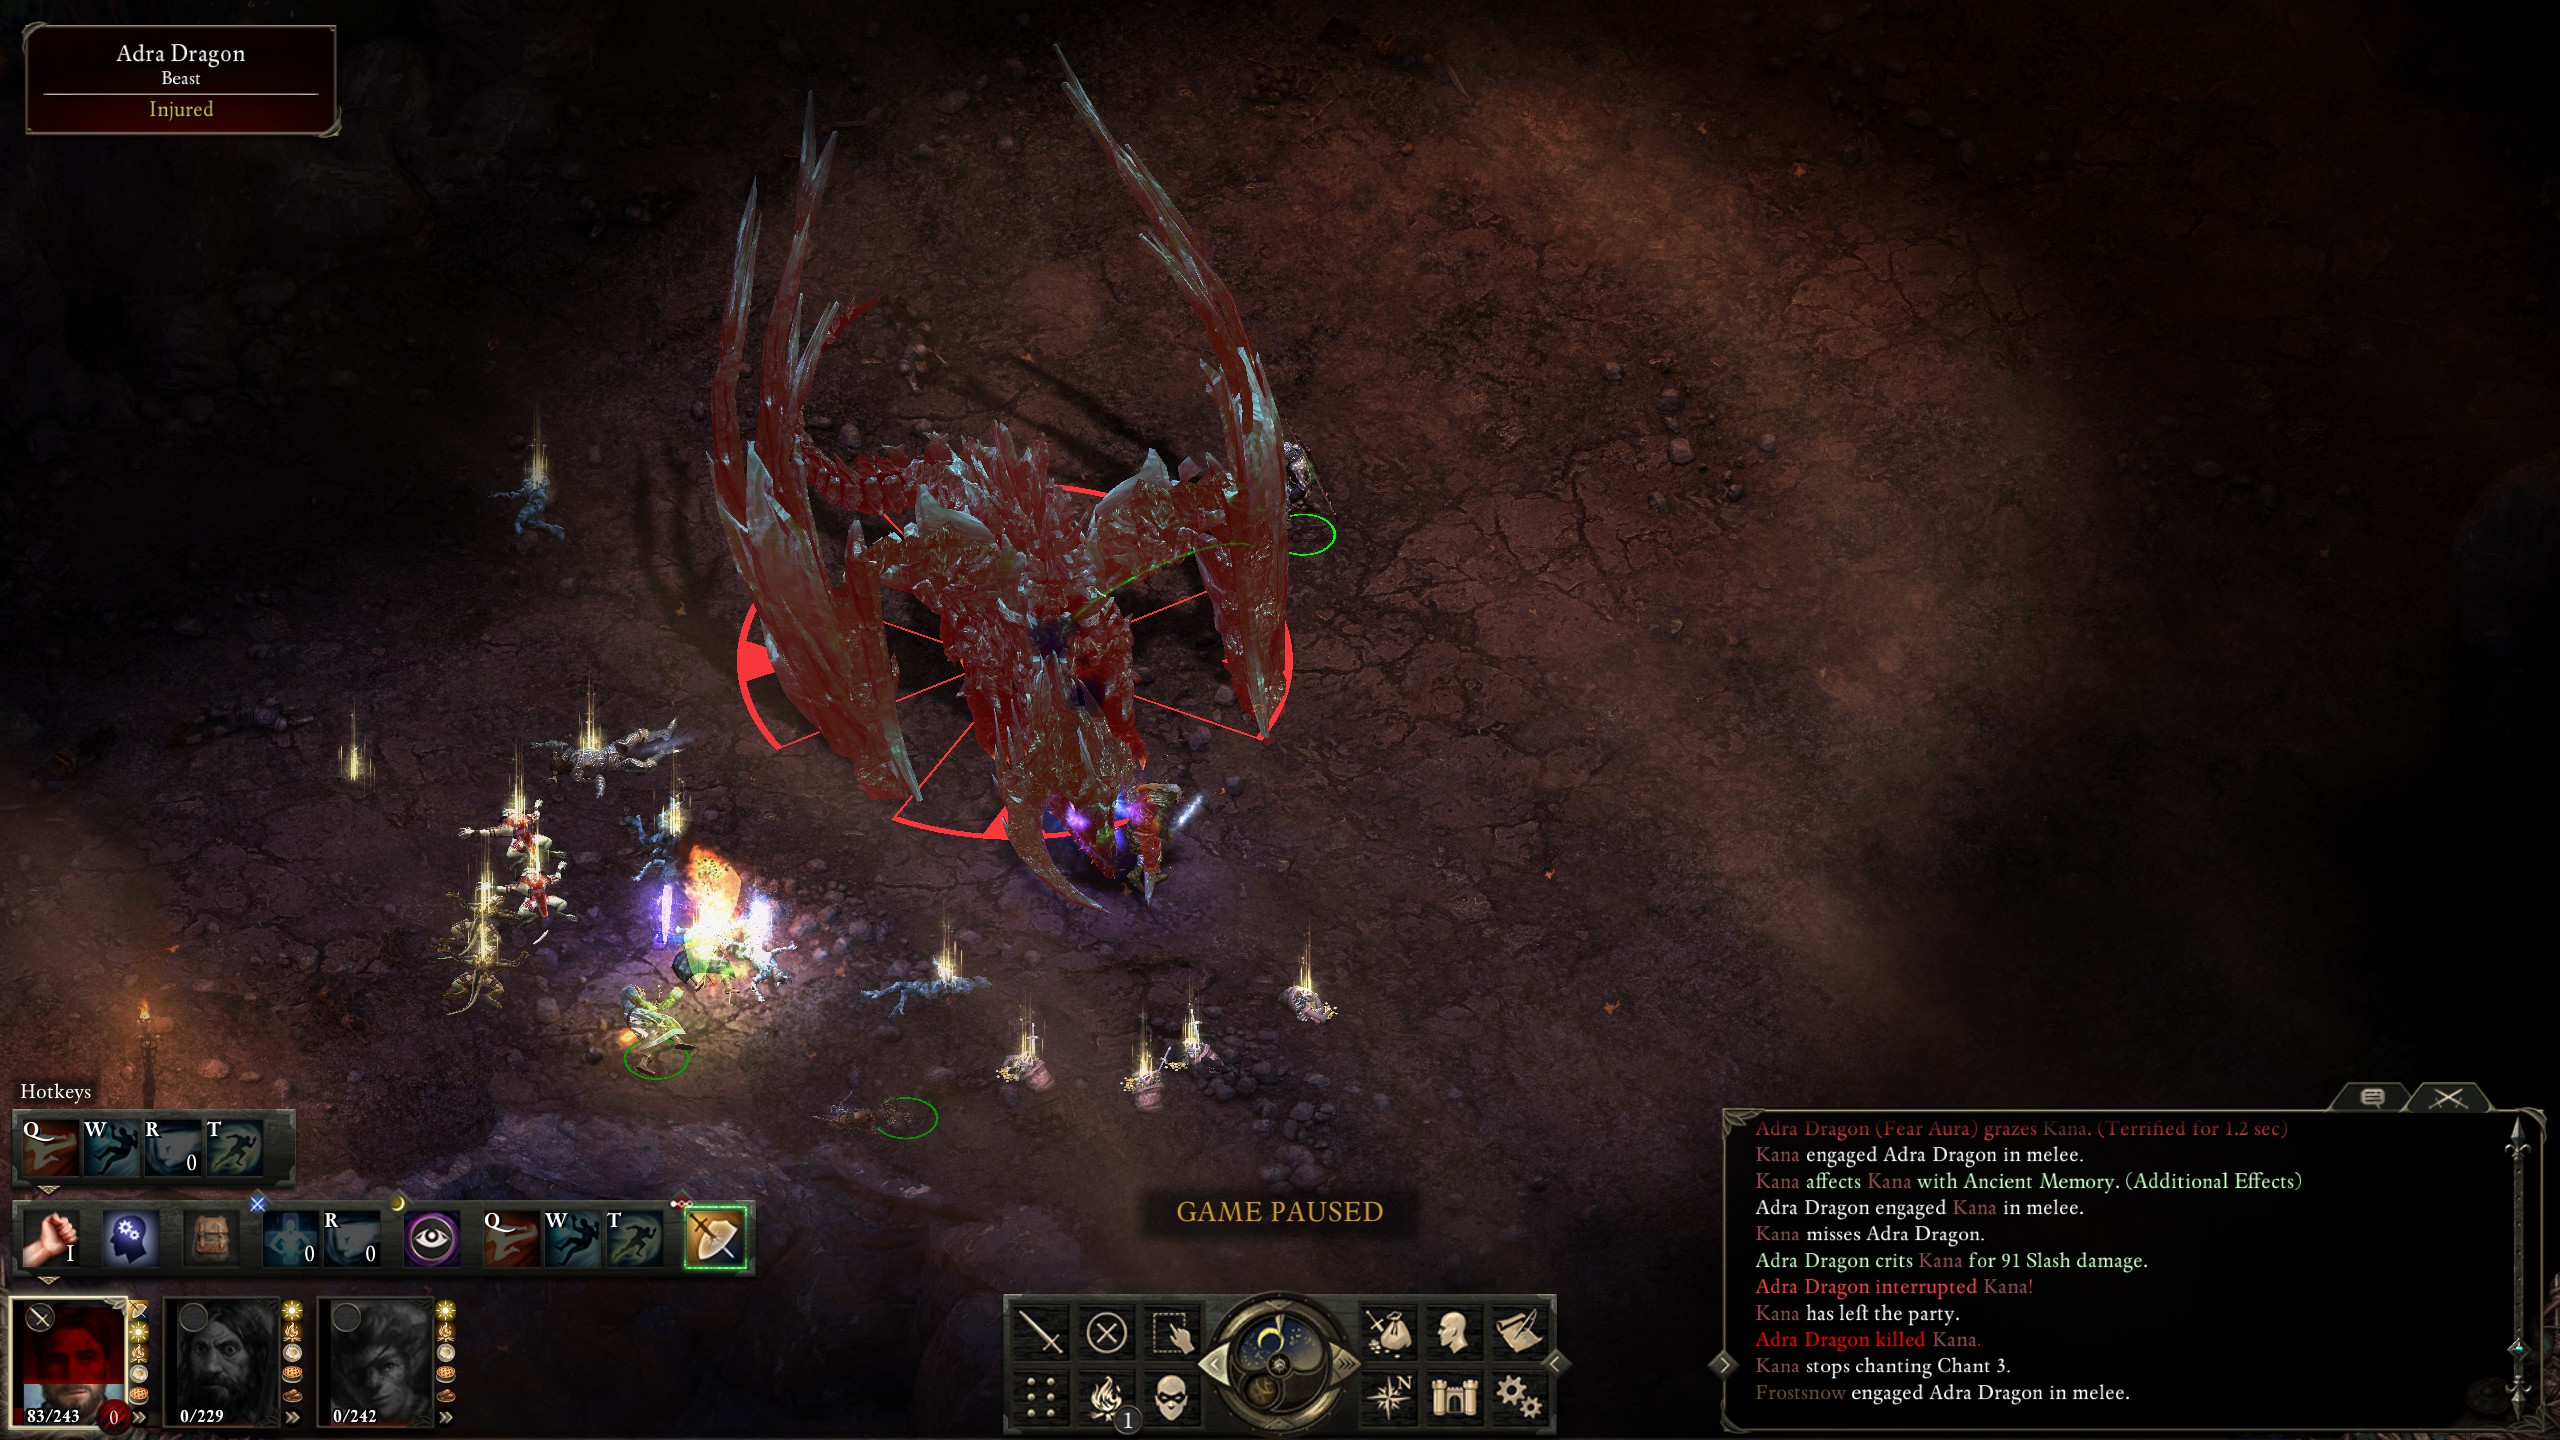
\includegraphics[scale=0.33]{files/blog/2019_03_17_pillars_of_eternity_path_of_the_damned_act_iv/2019_03_17_dragon1_11.jpg}
\end{figure}

My monk was then summarily crushed by the dragon's regular attacks.

\begin{figure}
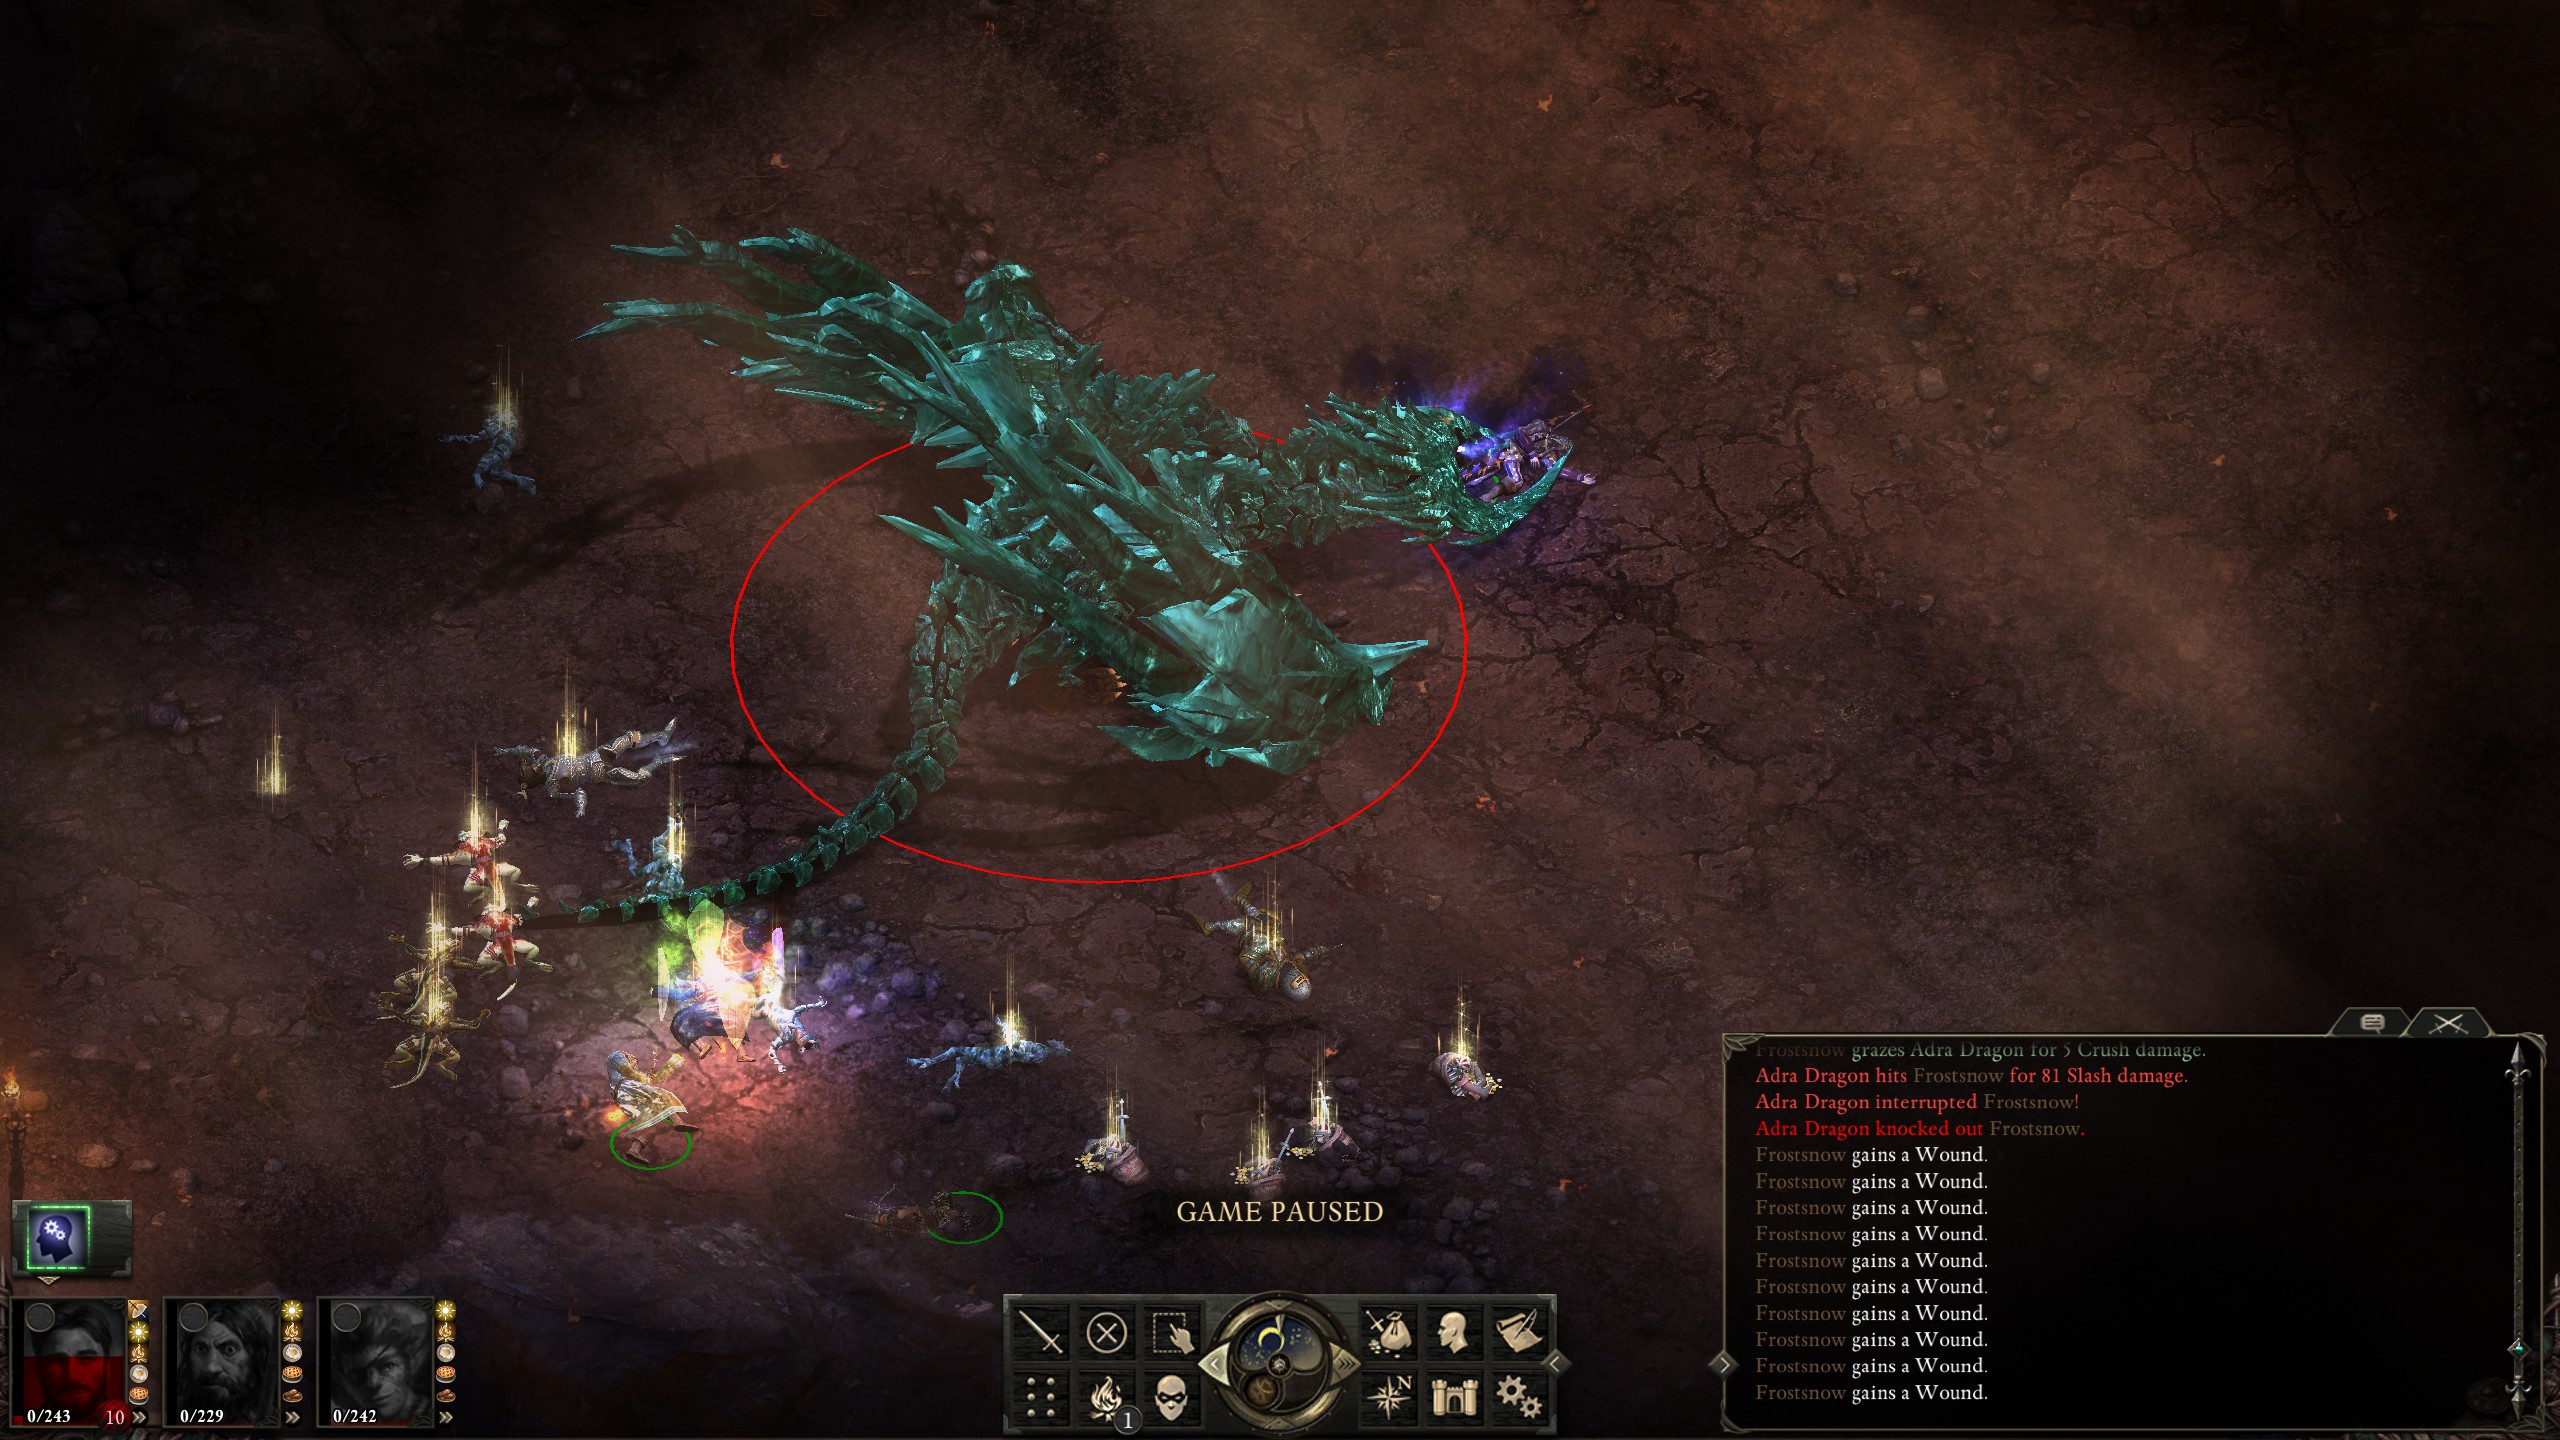
\includegraphics[scale=0.33]{files/blog/2019_03_17_pillars_of_eternity_path_of_the_damned_act_iv/2019_03_17_dragon1_12.jpg}
\end{figure}

Thus the first round went to the dragon.  Nearly my entire party had been \emph{killed} in what was probably the most brutal fight I'd ever experienced in the game.  I did make some decent strides against it, killing all of the adds and bringing it down to "Injured", but that was still pretty far from a victory.  I thought about what went wrong and decided that the \emph{initial} positioning had been wrong, though I couldn't think of a way to protect my entire party from dominates.  A few dominates would probably do less damage than a Wing Slam plus Breath attack combo, though.

\subsubsection{Attempt #2}

For my second attempt I decided to send Eder in alone while I had Durance protect the rest of the team.  This ran the risk of Eder getting dominated and messing up my positioning, but I couldn't think of any better option.

\begin{figure}
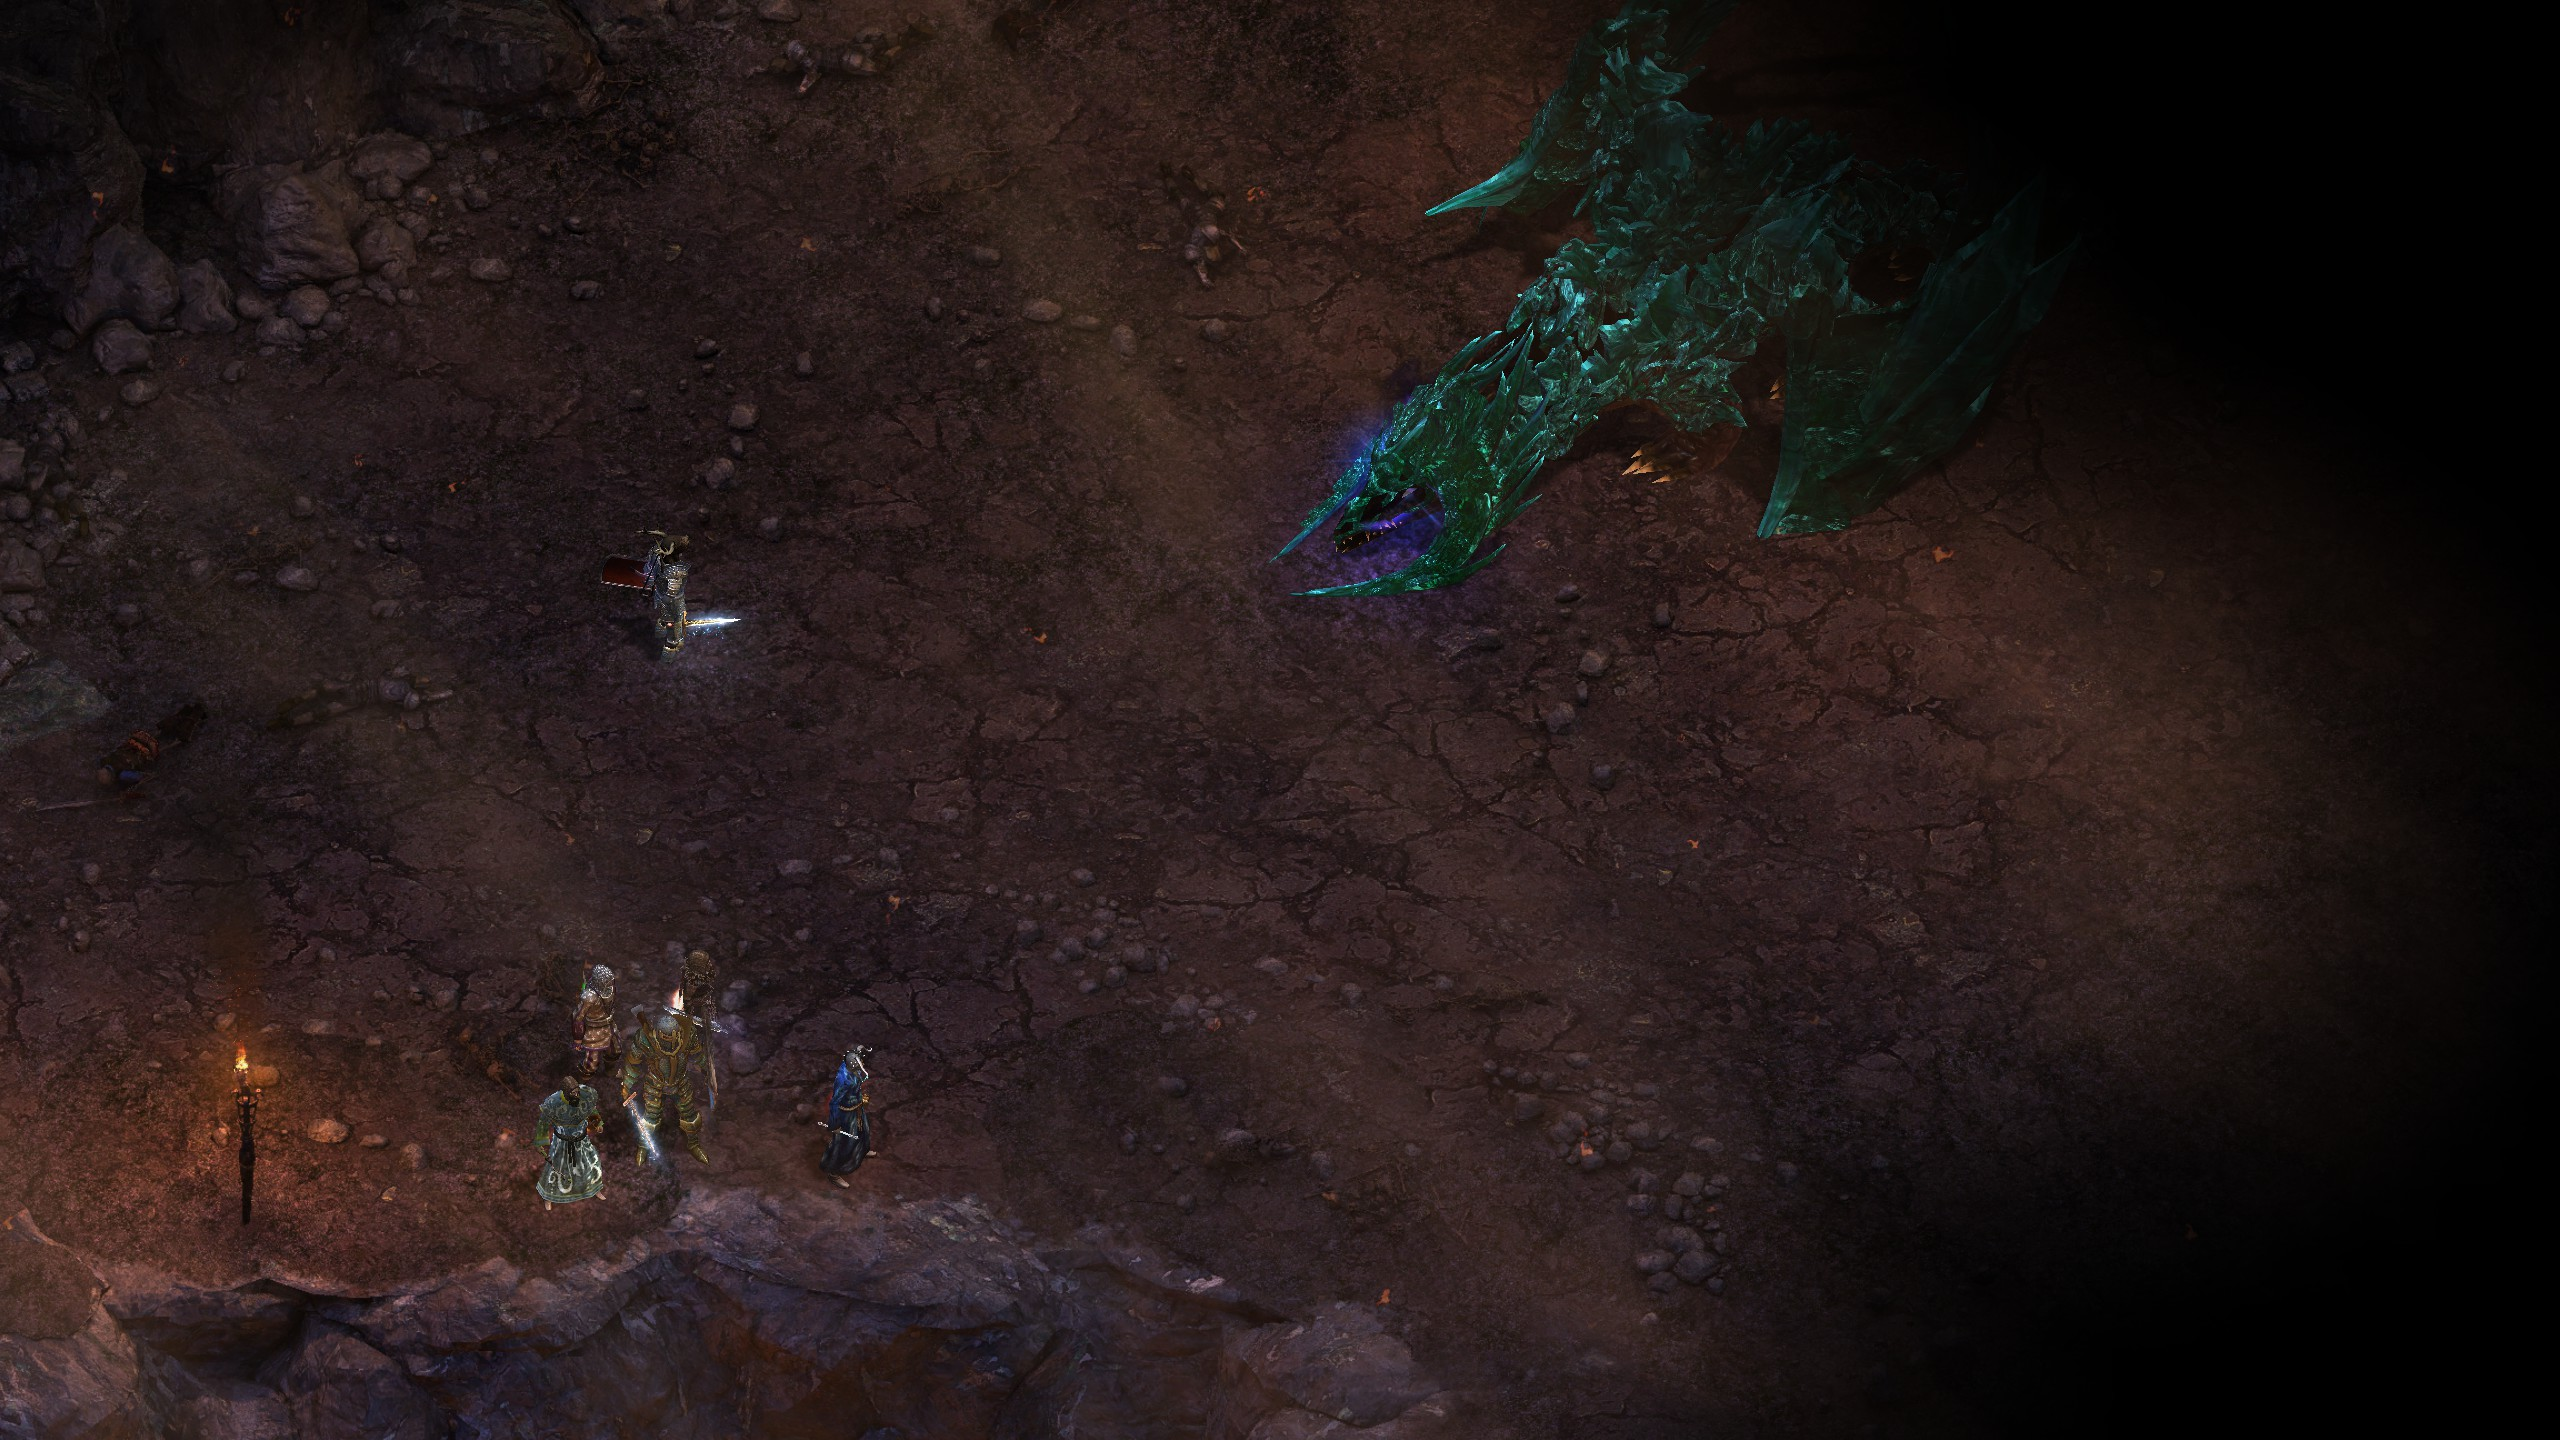
\includegraphics[scale=0.33]{files/blog/2019_03_17_pillars_of_eternity_path_of_the_damned_act_iv/2019_03_17_dragon2_01.jpg}
\end{figure}

It started out well enough.  The dragon missed its Wing Slam while I summoned a few extra minions and decided to apply a few more buffs.

\begin{figure}
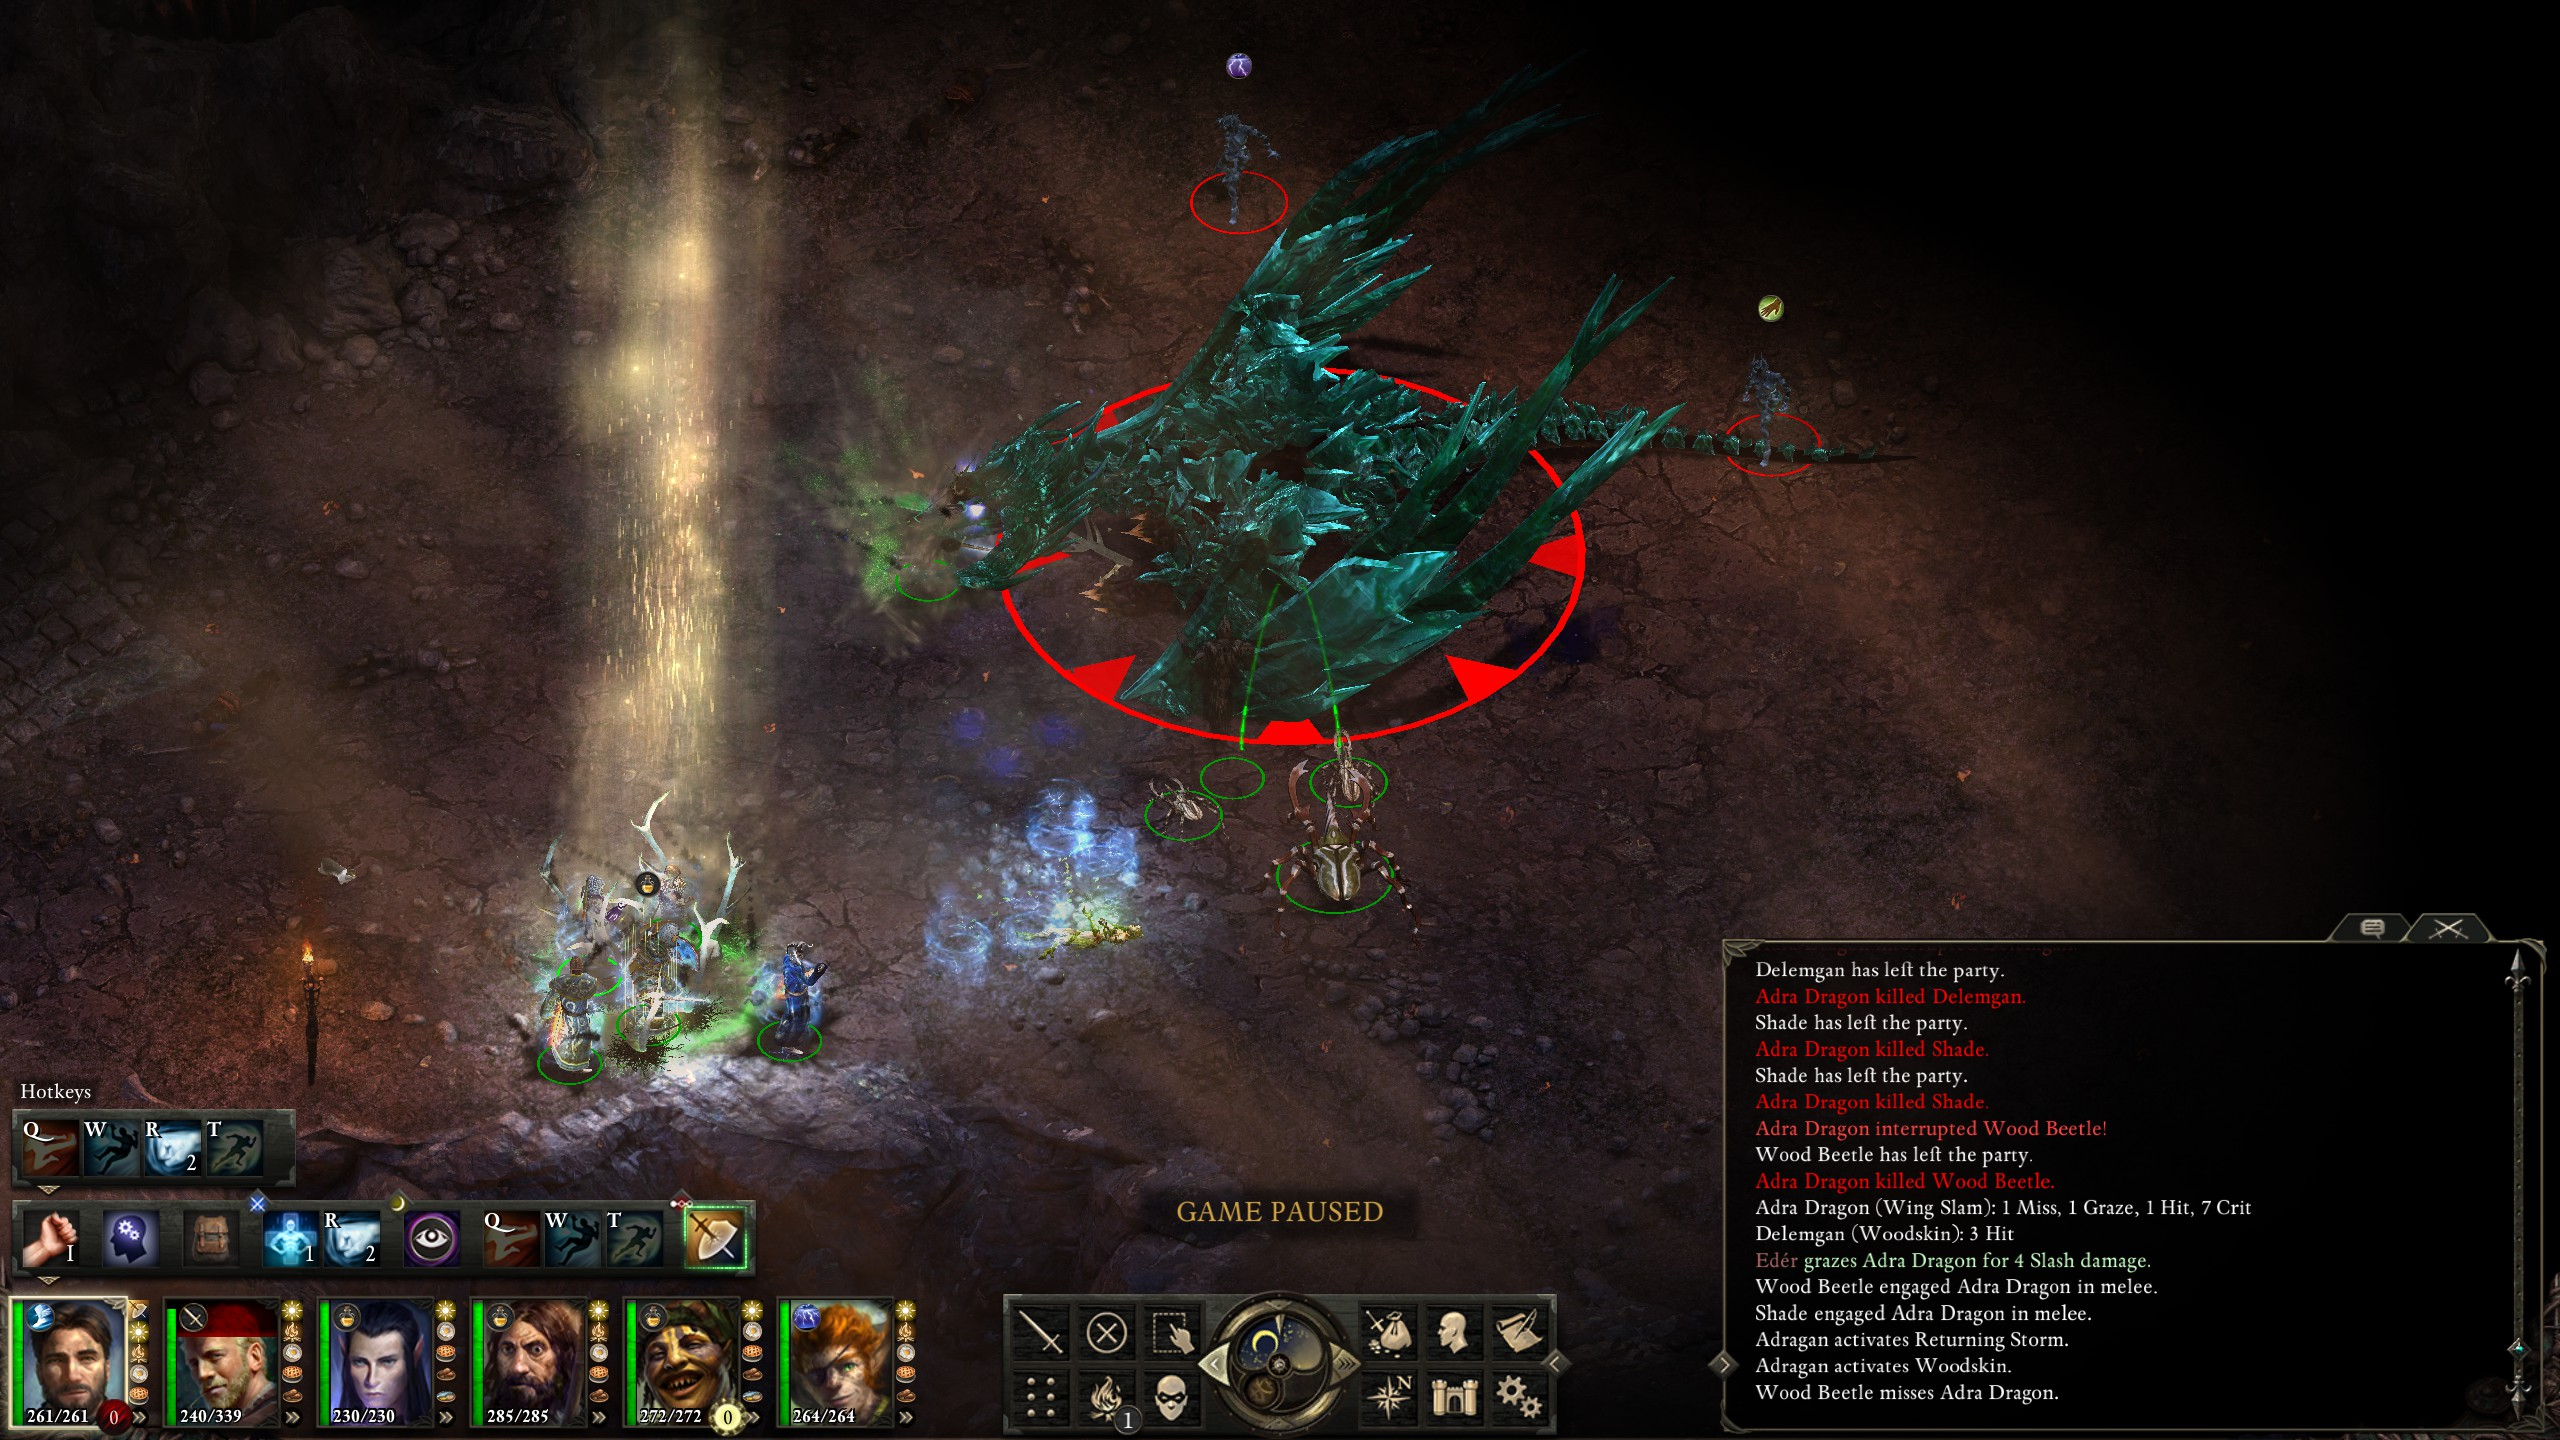
\includegraphics[scale=0.33]{files/blog/2019_03_17_pillars_of_eternity_path_of_the_damned_act_iv/2019_03_17_dragon2_02.jpg}
\end{figure}

That turned out to be a bad idea.  While the Wing Slam missed, the breath attack certainly didn't.

\begin{figure}
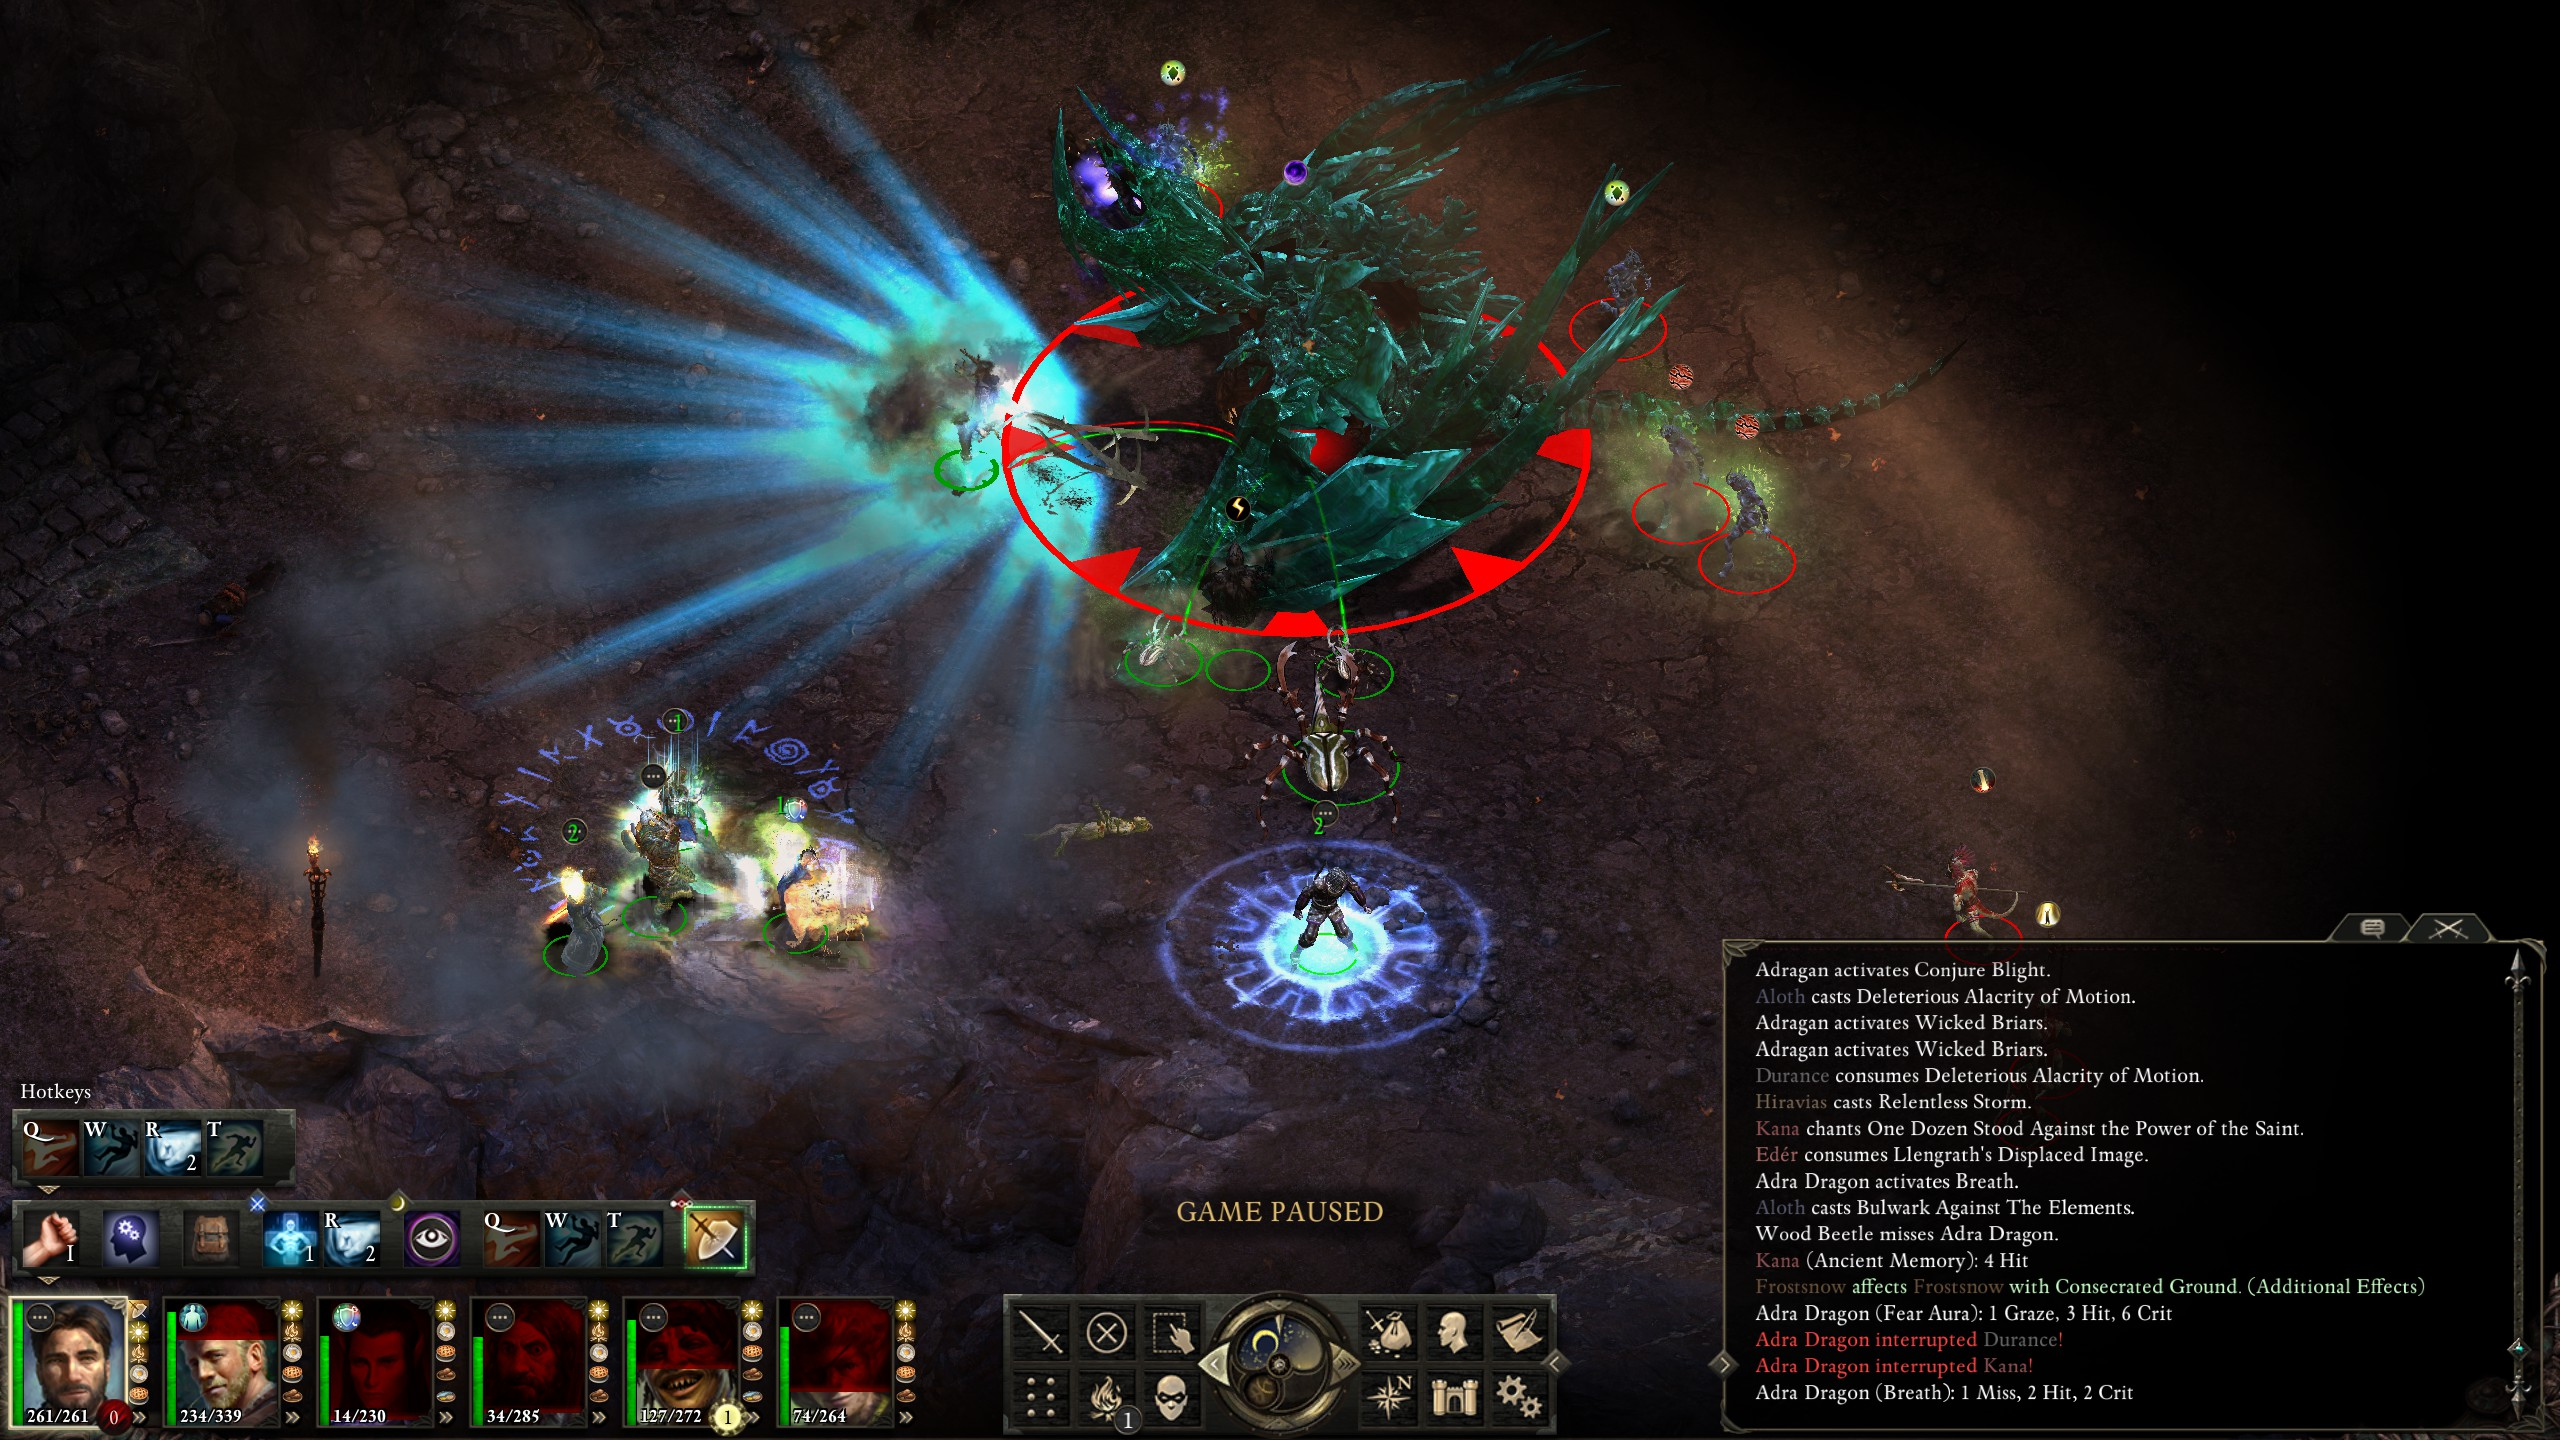
\includegraphics[scale=0.33]{files/blog/2019_03_17_pillars_of_eternity_path_of_the_damned_act_iv/2019_03_17_dragon2_03.jpg}
\end{figure}

I quickly got into a proper position after that.

\begin{figure}
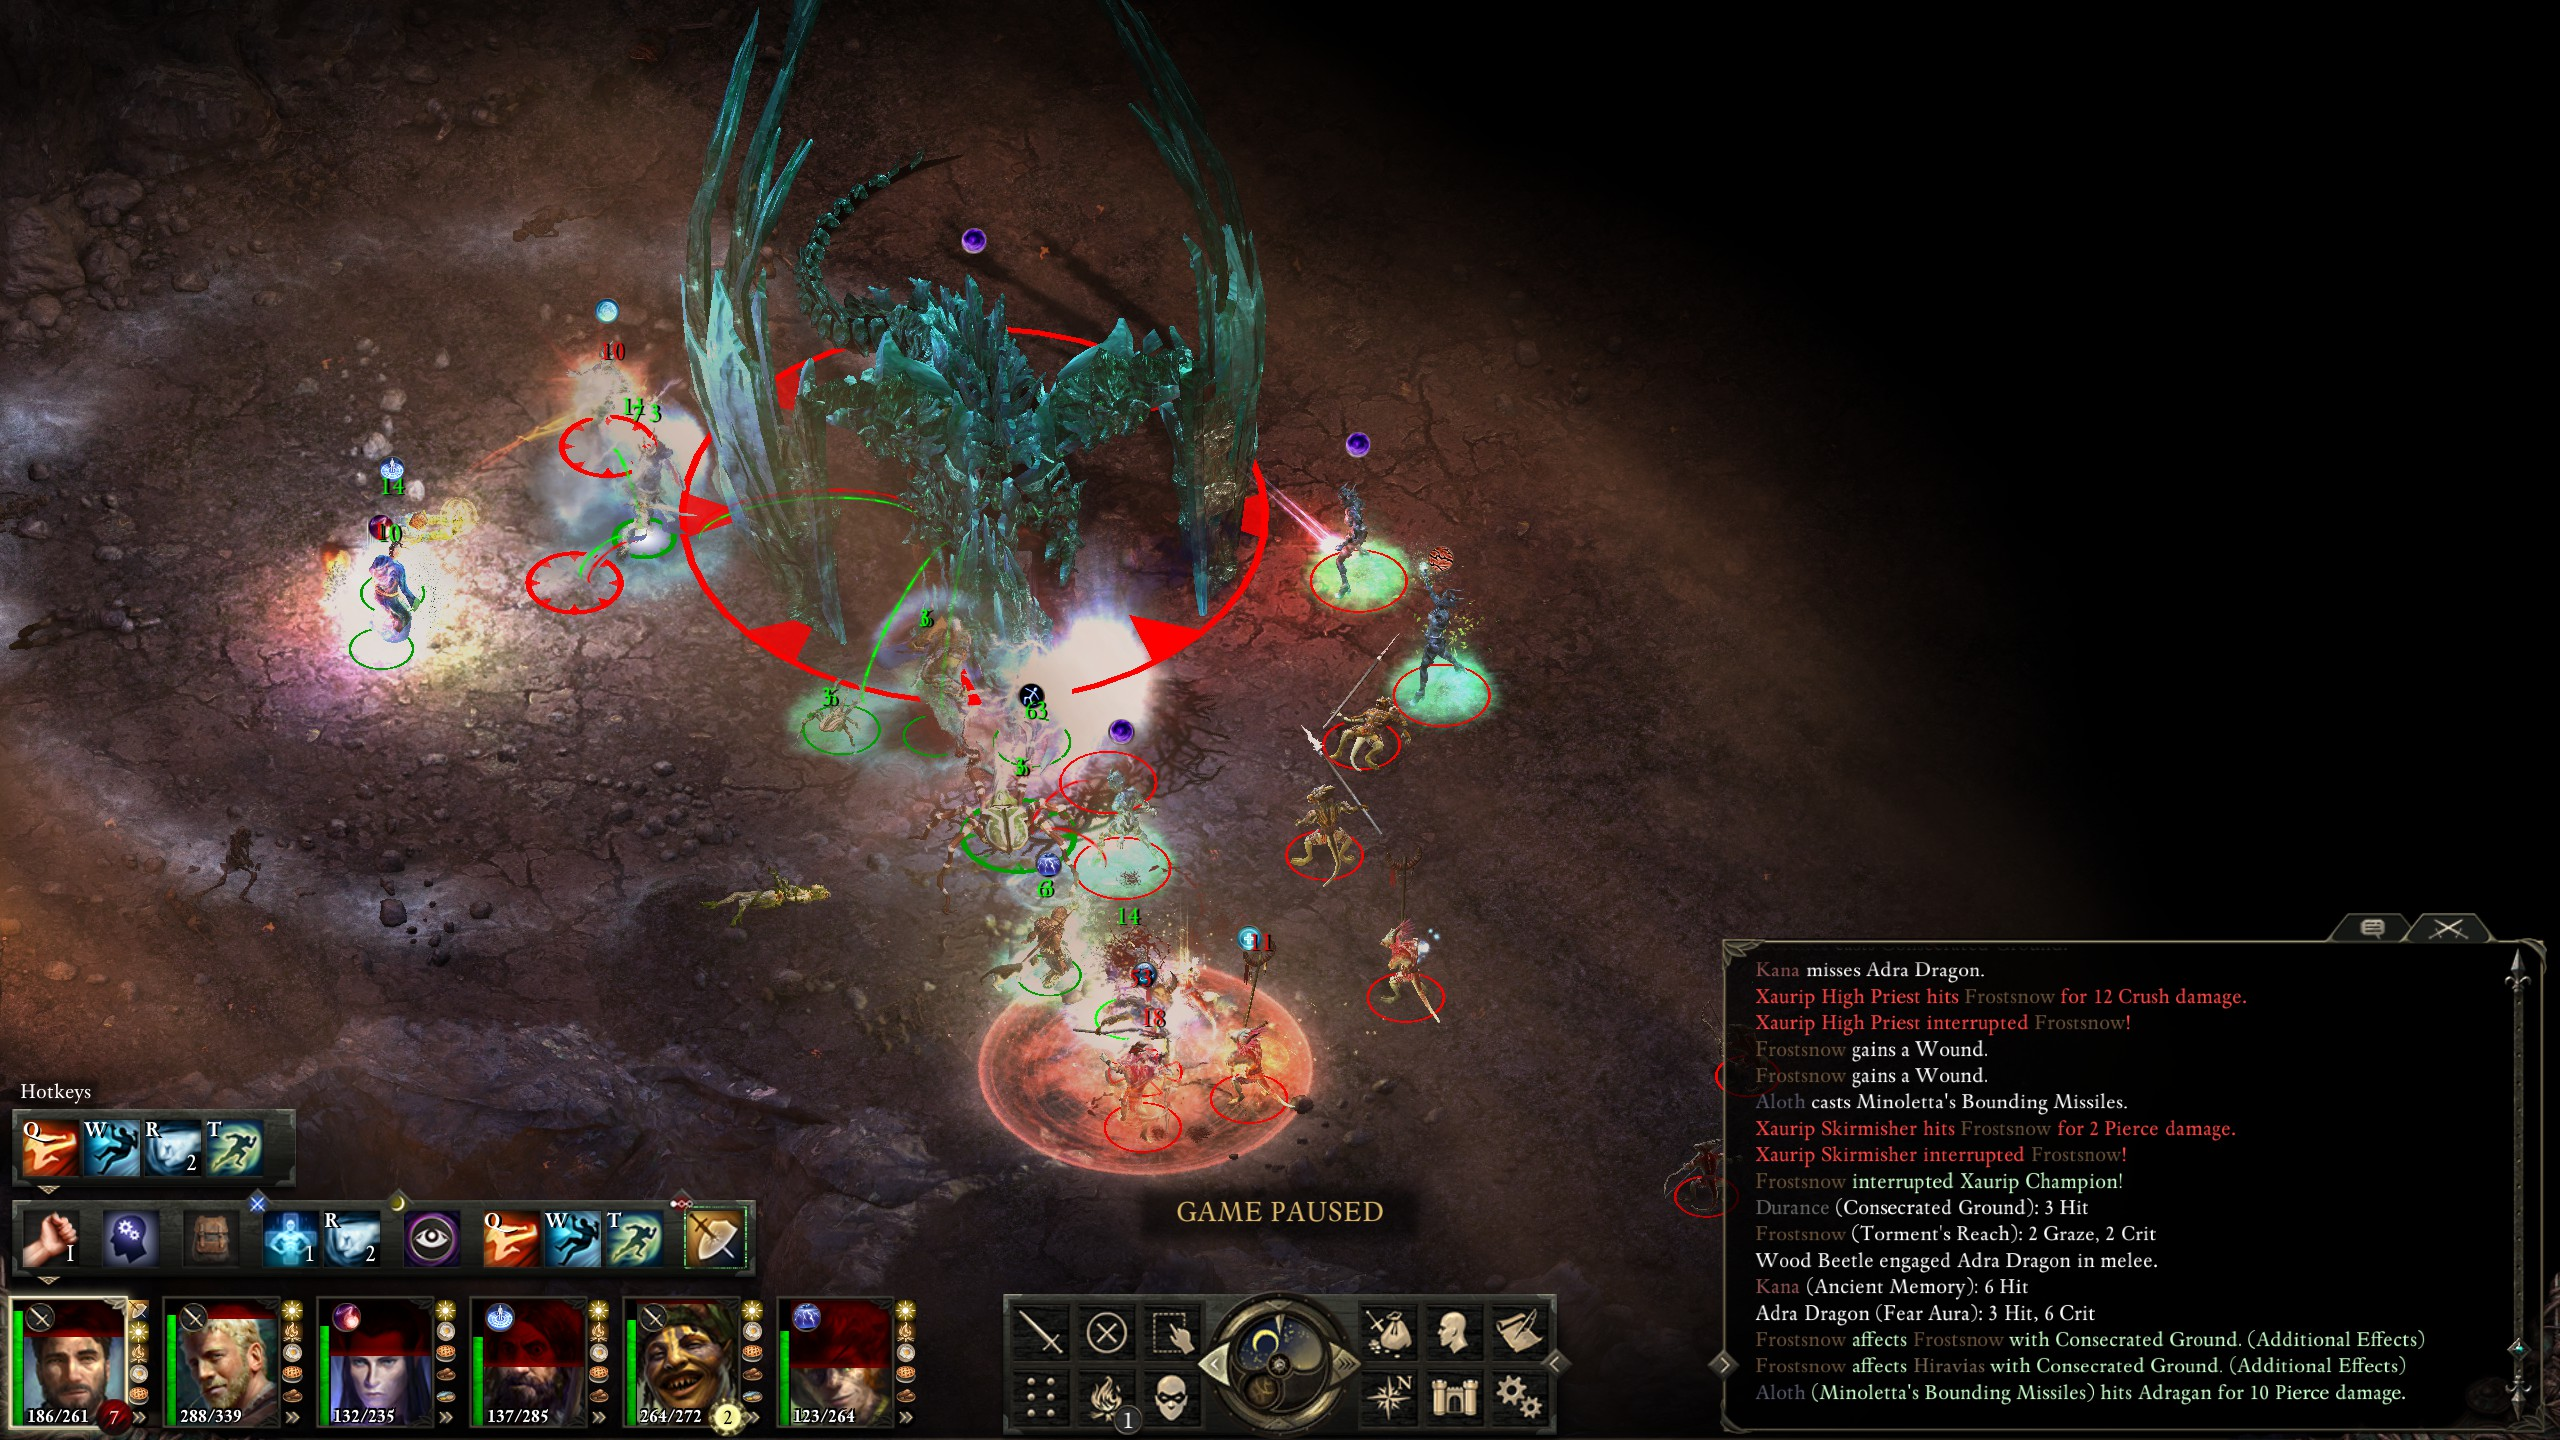
\includegraphics[scale=0.33]{files/blog/2019_03_17_pillars_of_eternity_path_of_the_damned_act_iv/2019_03_17_dragon2_04.jpg}
\end{figure}

It was taking longer than I'd have liked for Hiravas and my Monk to kills the adds, so I decided to send Aloth in to help.

\begin{figure}
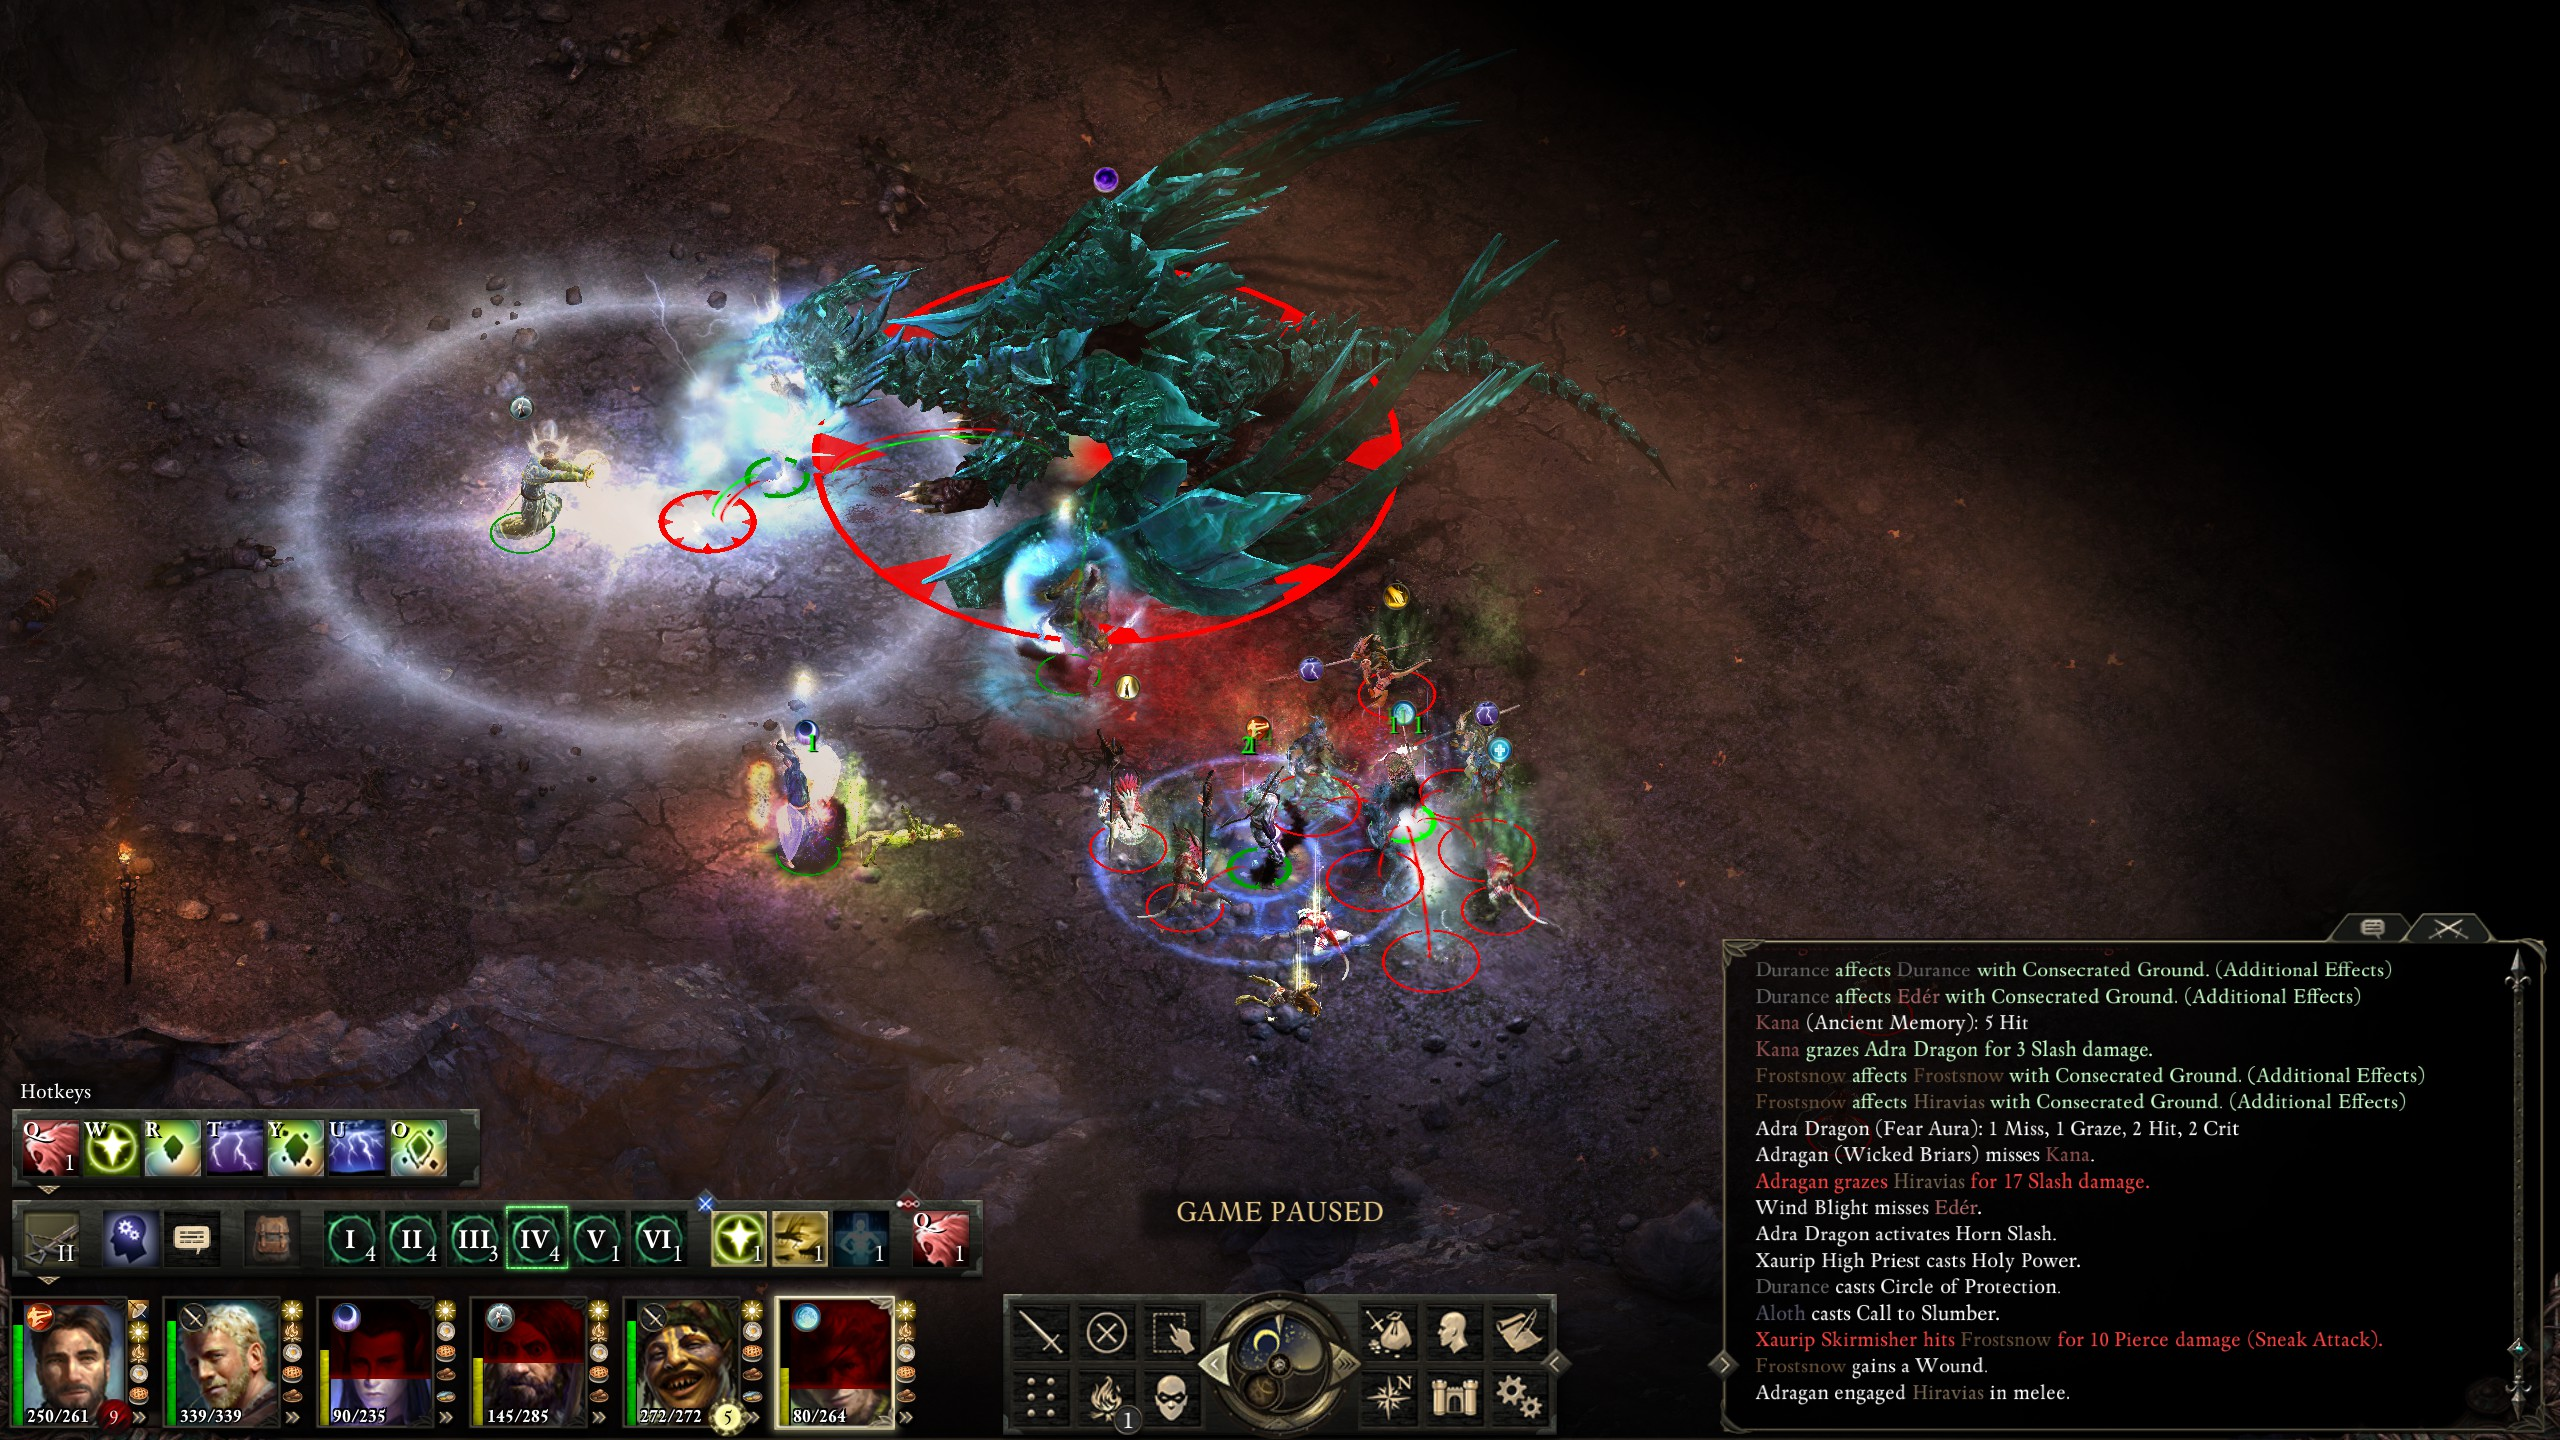
\includegraphics[scale=0.33]{files/blog/2019_03_17_pillars_of_eternity_path_of_the_damned_act_iv/2019_03_17_dragon2_05.jpg}
\end{figure}

I used the "Call to Slumber" followed my "Minoletta's Precisely Piercing Burst" combo I'd learned from the first fight in order to make quick work of the xaurips.

\begin{figure}
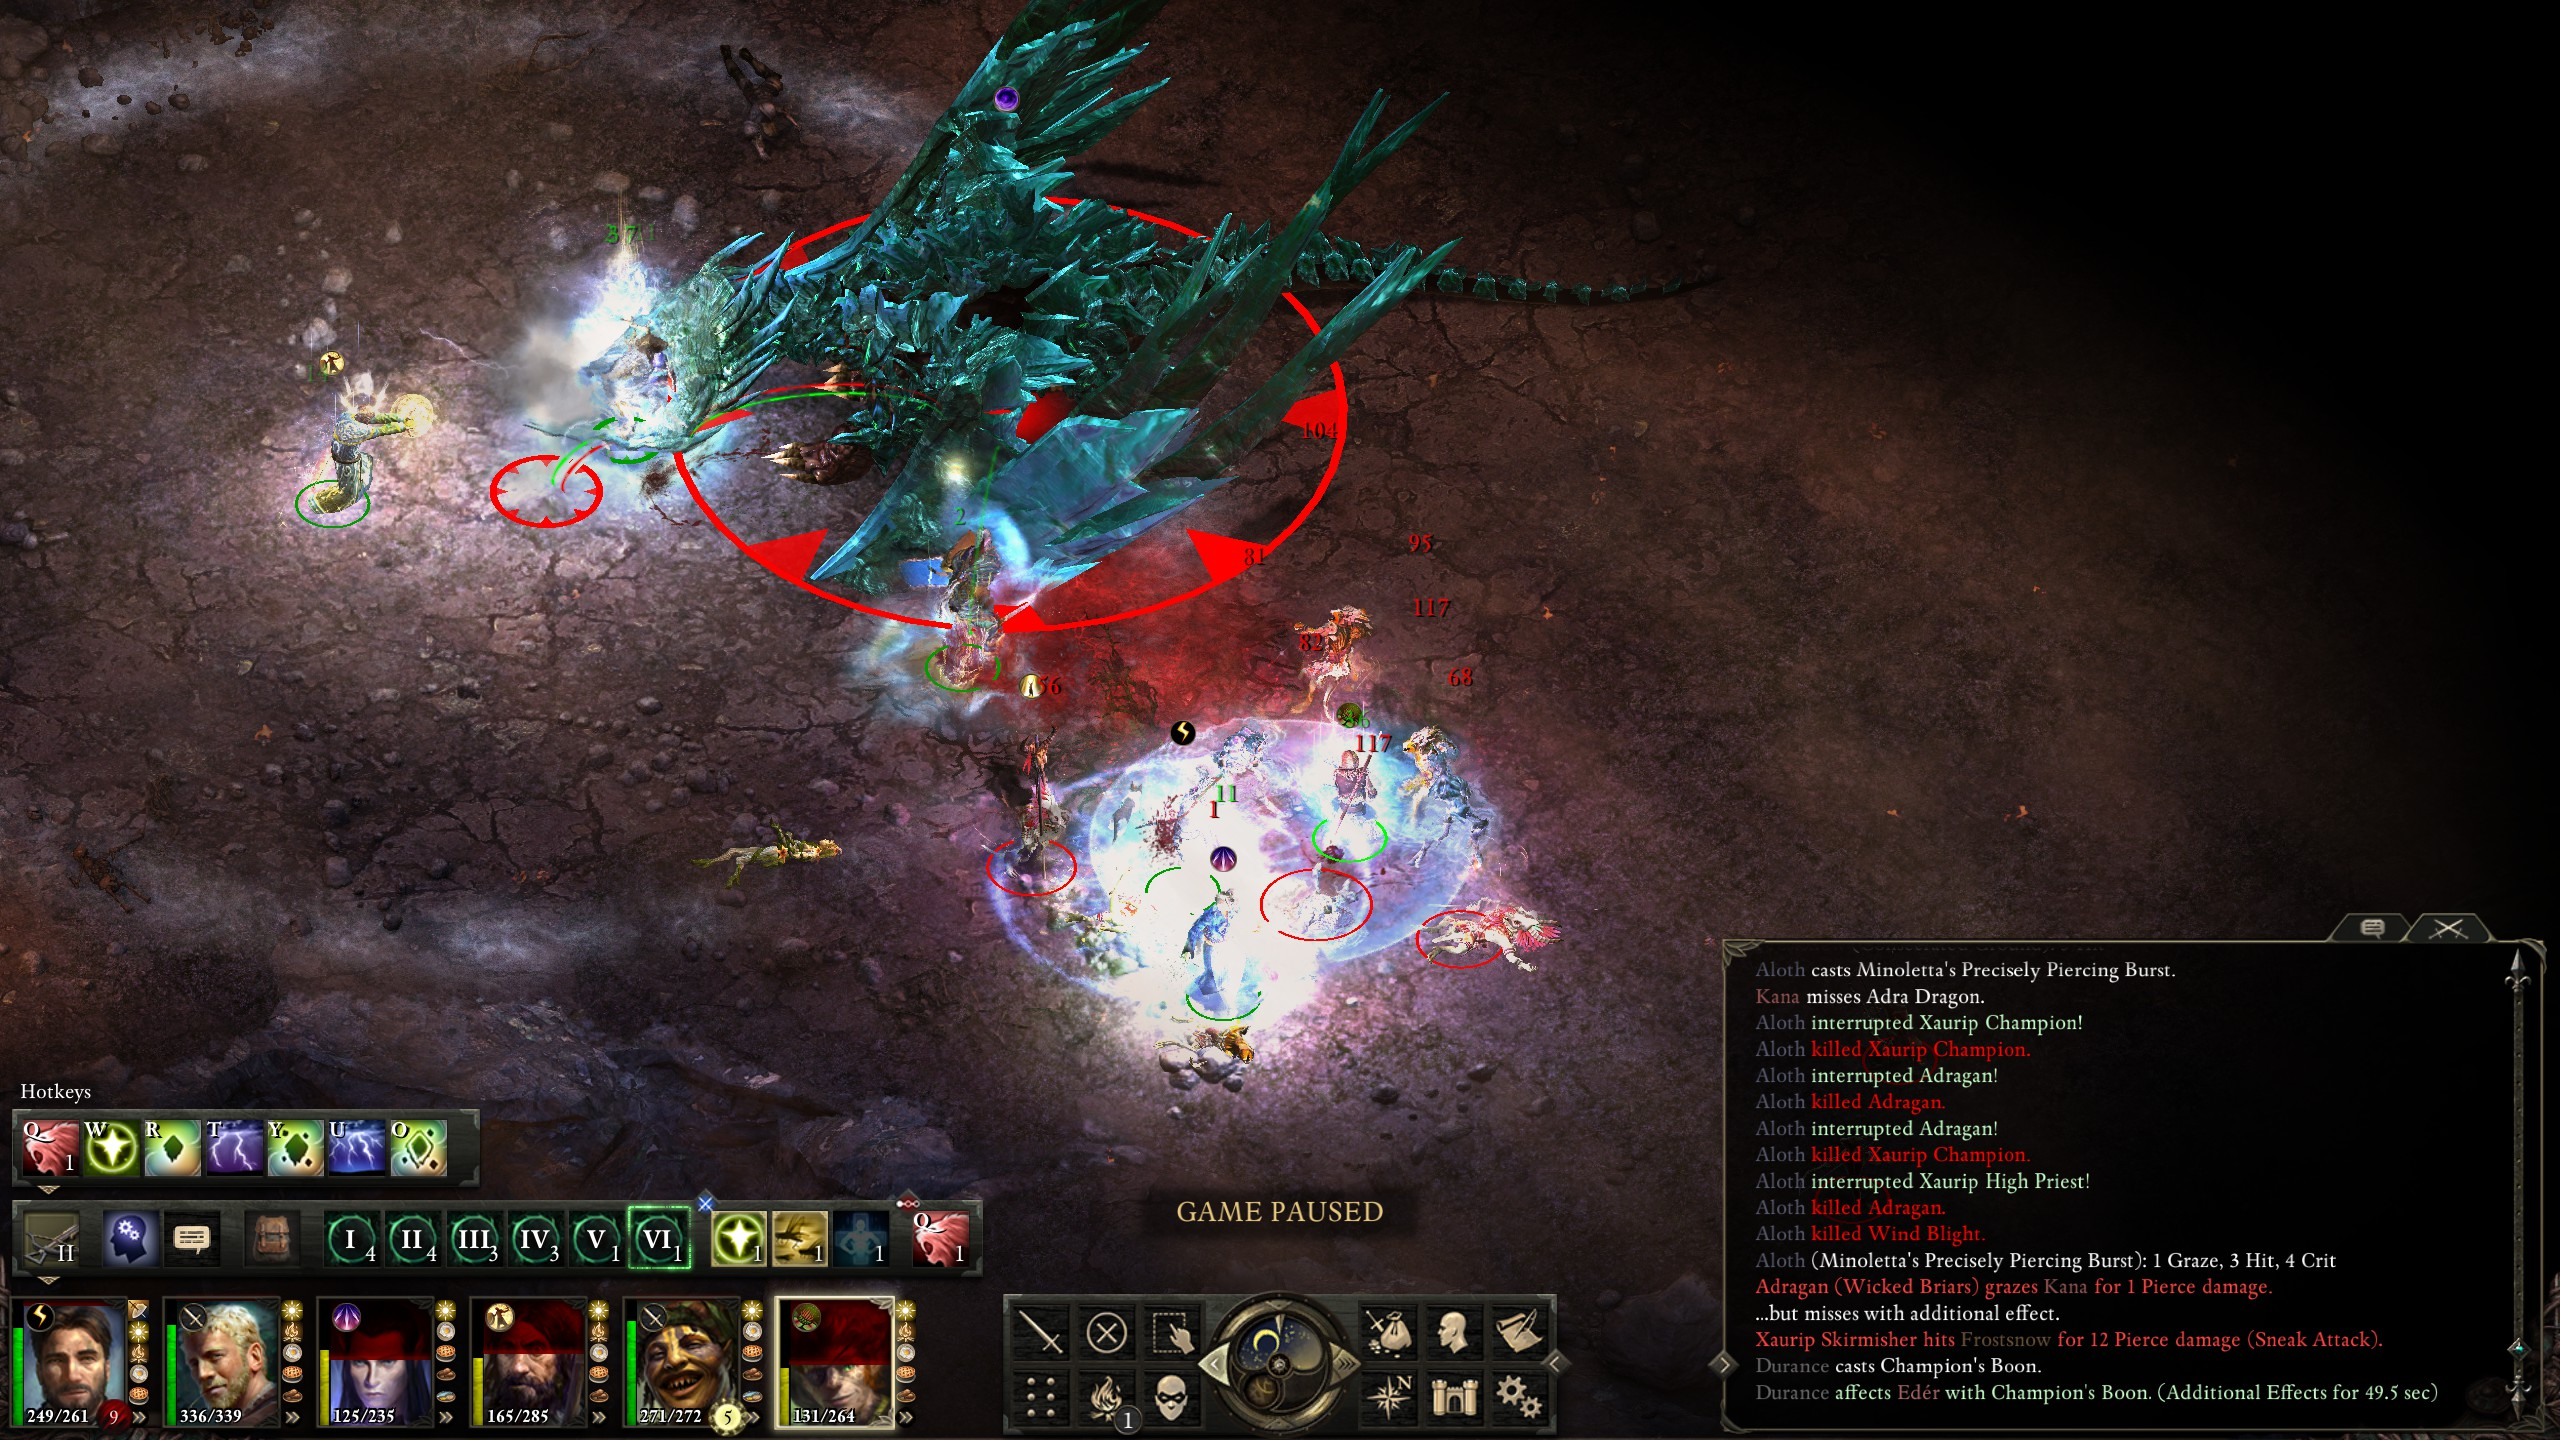
\includegraphics[scale=0.33]{files/blog/2019_03_17_pillars_of_eternity_path_of_the_damned_act_iv/2019_03_17_dragon2_06.jpg}
\end{figure}

My two-subgroup strategy appeared to be working, as the dragon then threw a breath attack that was only able to hit one group.

\begin{figure}
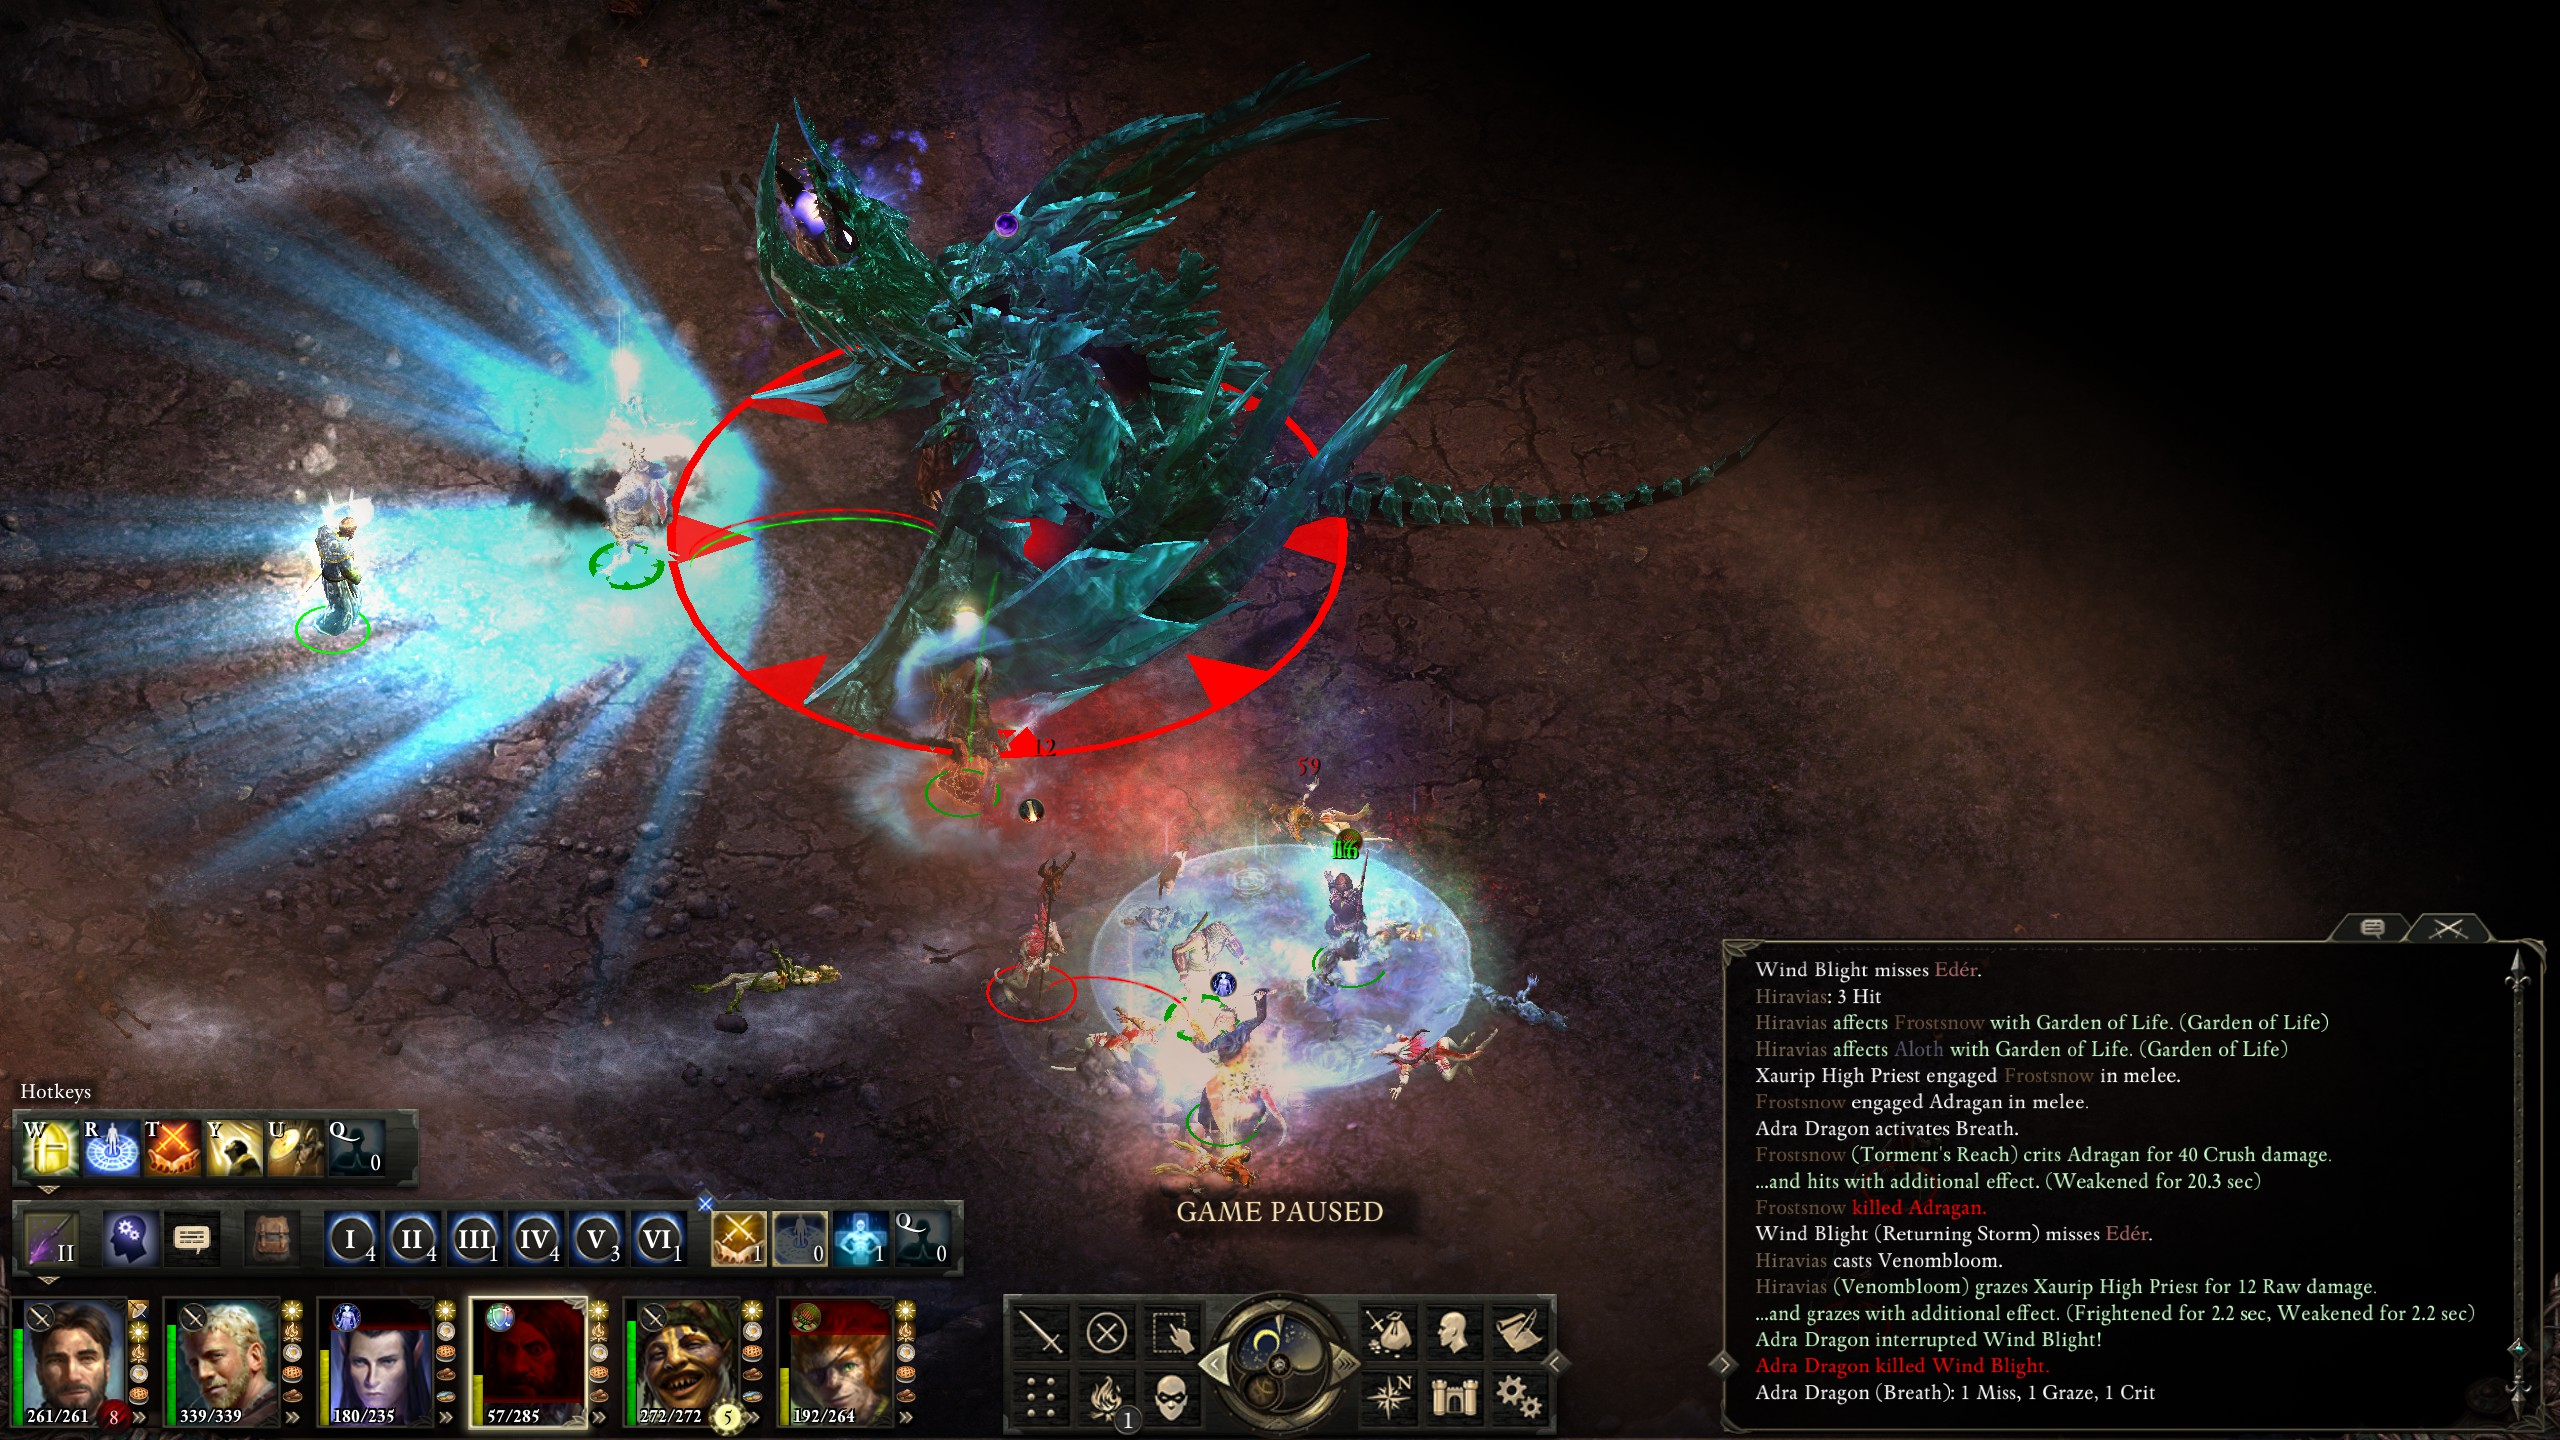
\includegraphics[scale=0.33]{files/blog/2019_03_17_pillars_of_eternity_path_of_the_damned_act_iv/2019_03_17_dragon2_07.jpg}
\end{figure}

Unfortunately for Durance, he wasn't able to heal up in time to make it through the coming Wing Slam critical that would then land on him.

\begin{figure}
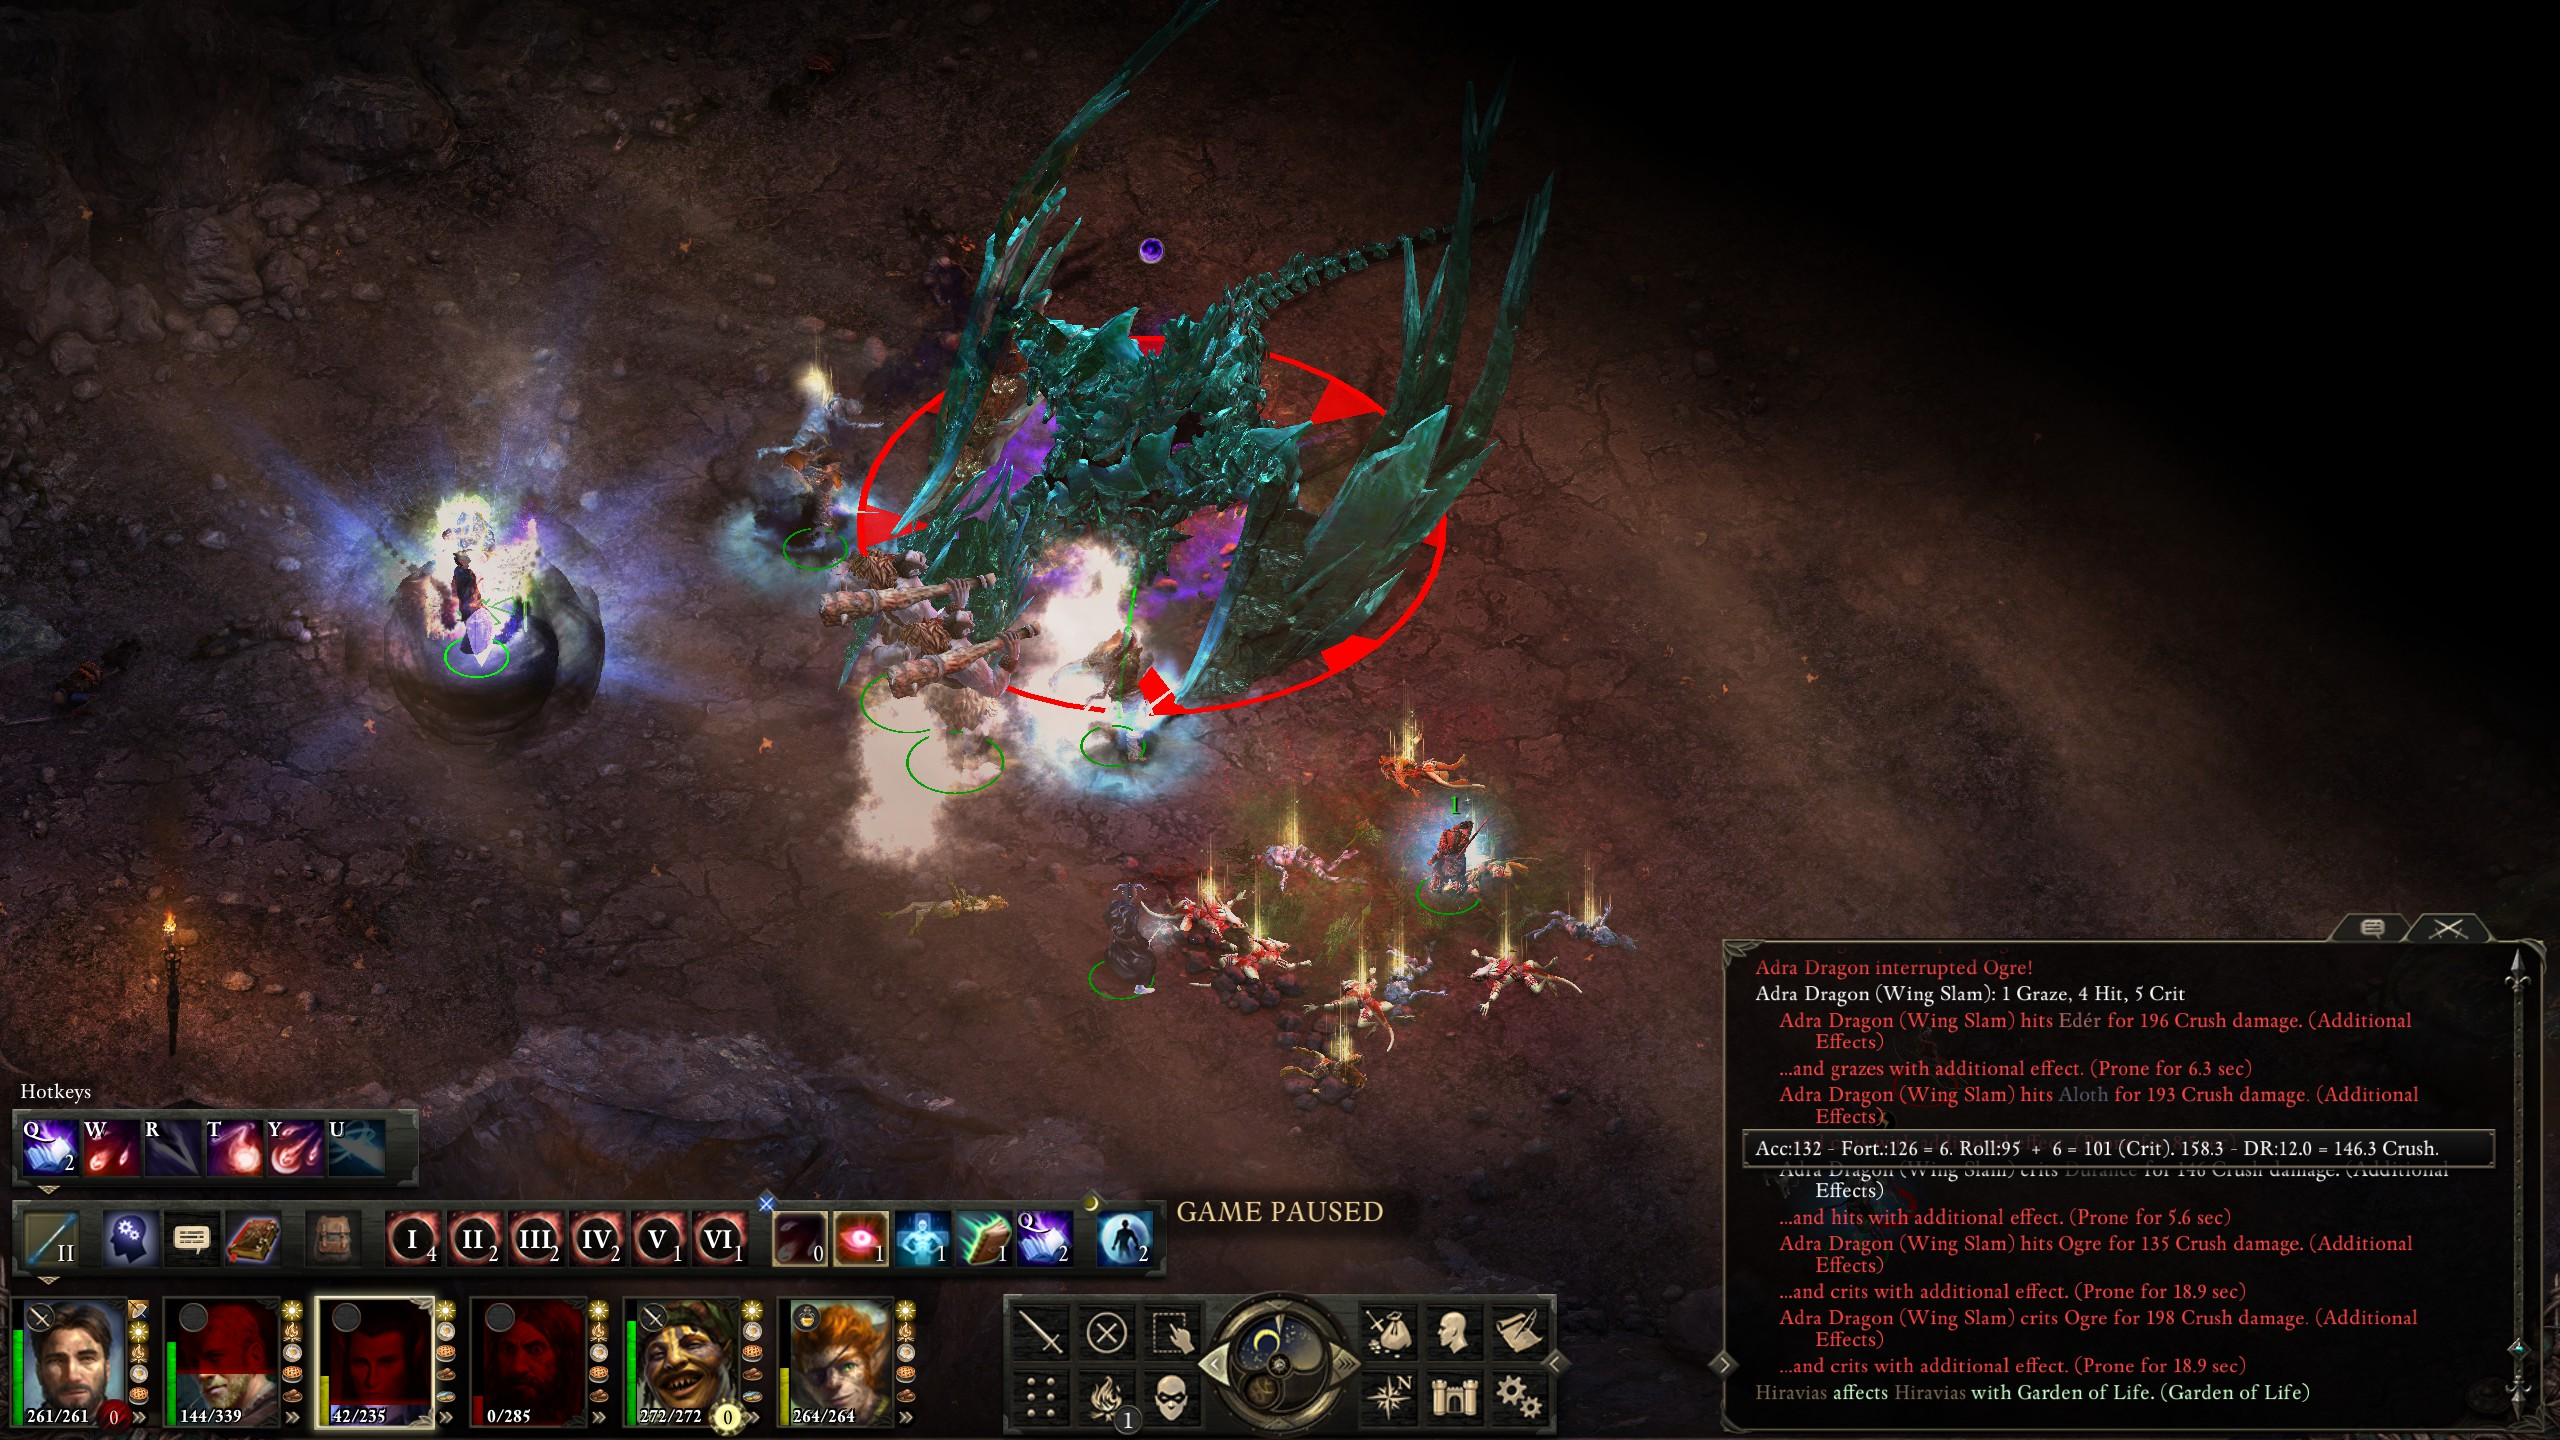
\includegraphics[scale=0.33]{files/blog/2019_03_17_pillars_of_eternity_path_of_the_damned_act_iv/2019_03_17_dragon2_08.jpg}
\end{figure}

That was okay, though, as he had the "Second Chance" enchantment on his robe and Aloth and Hiravas were both capable of reviving him if the enchantment was down.  A short while later he was up, healed, and casting more buffs.

\begin{figure}
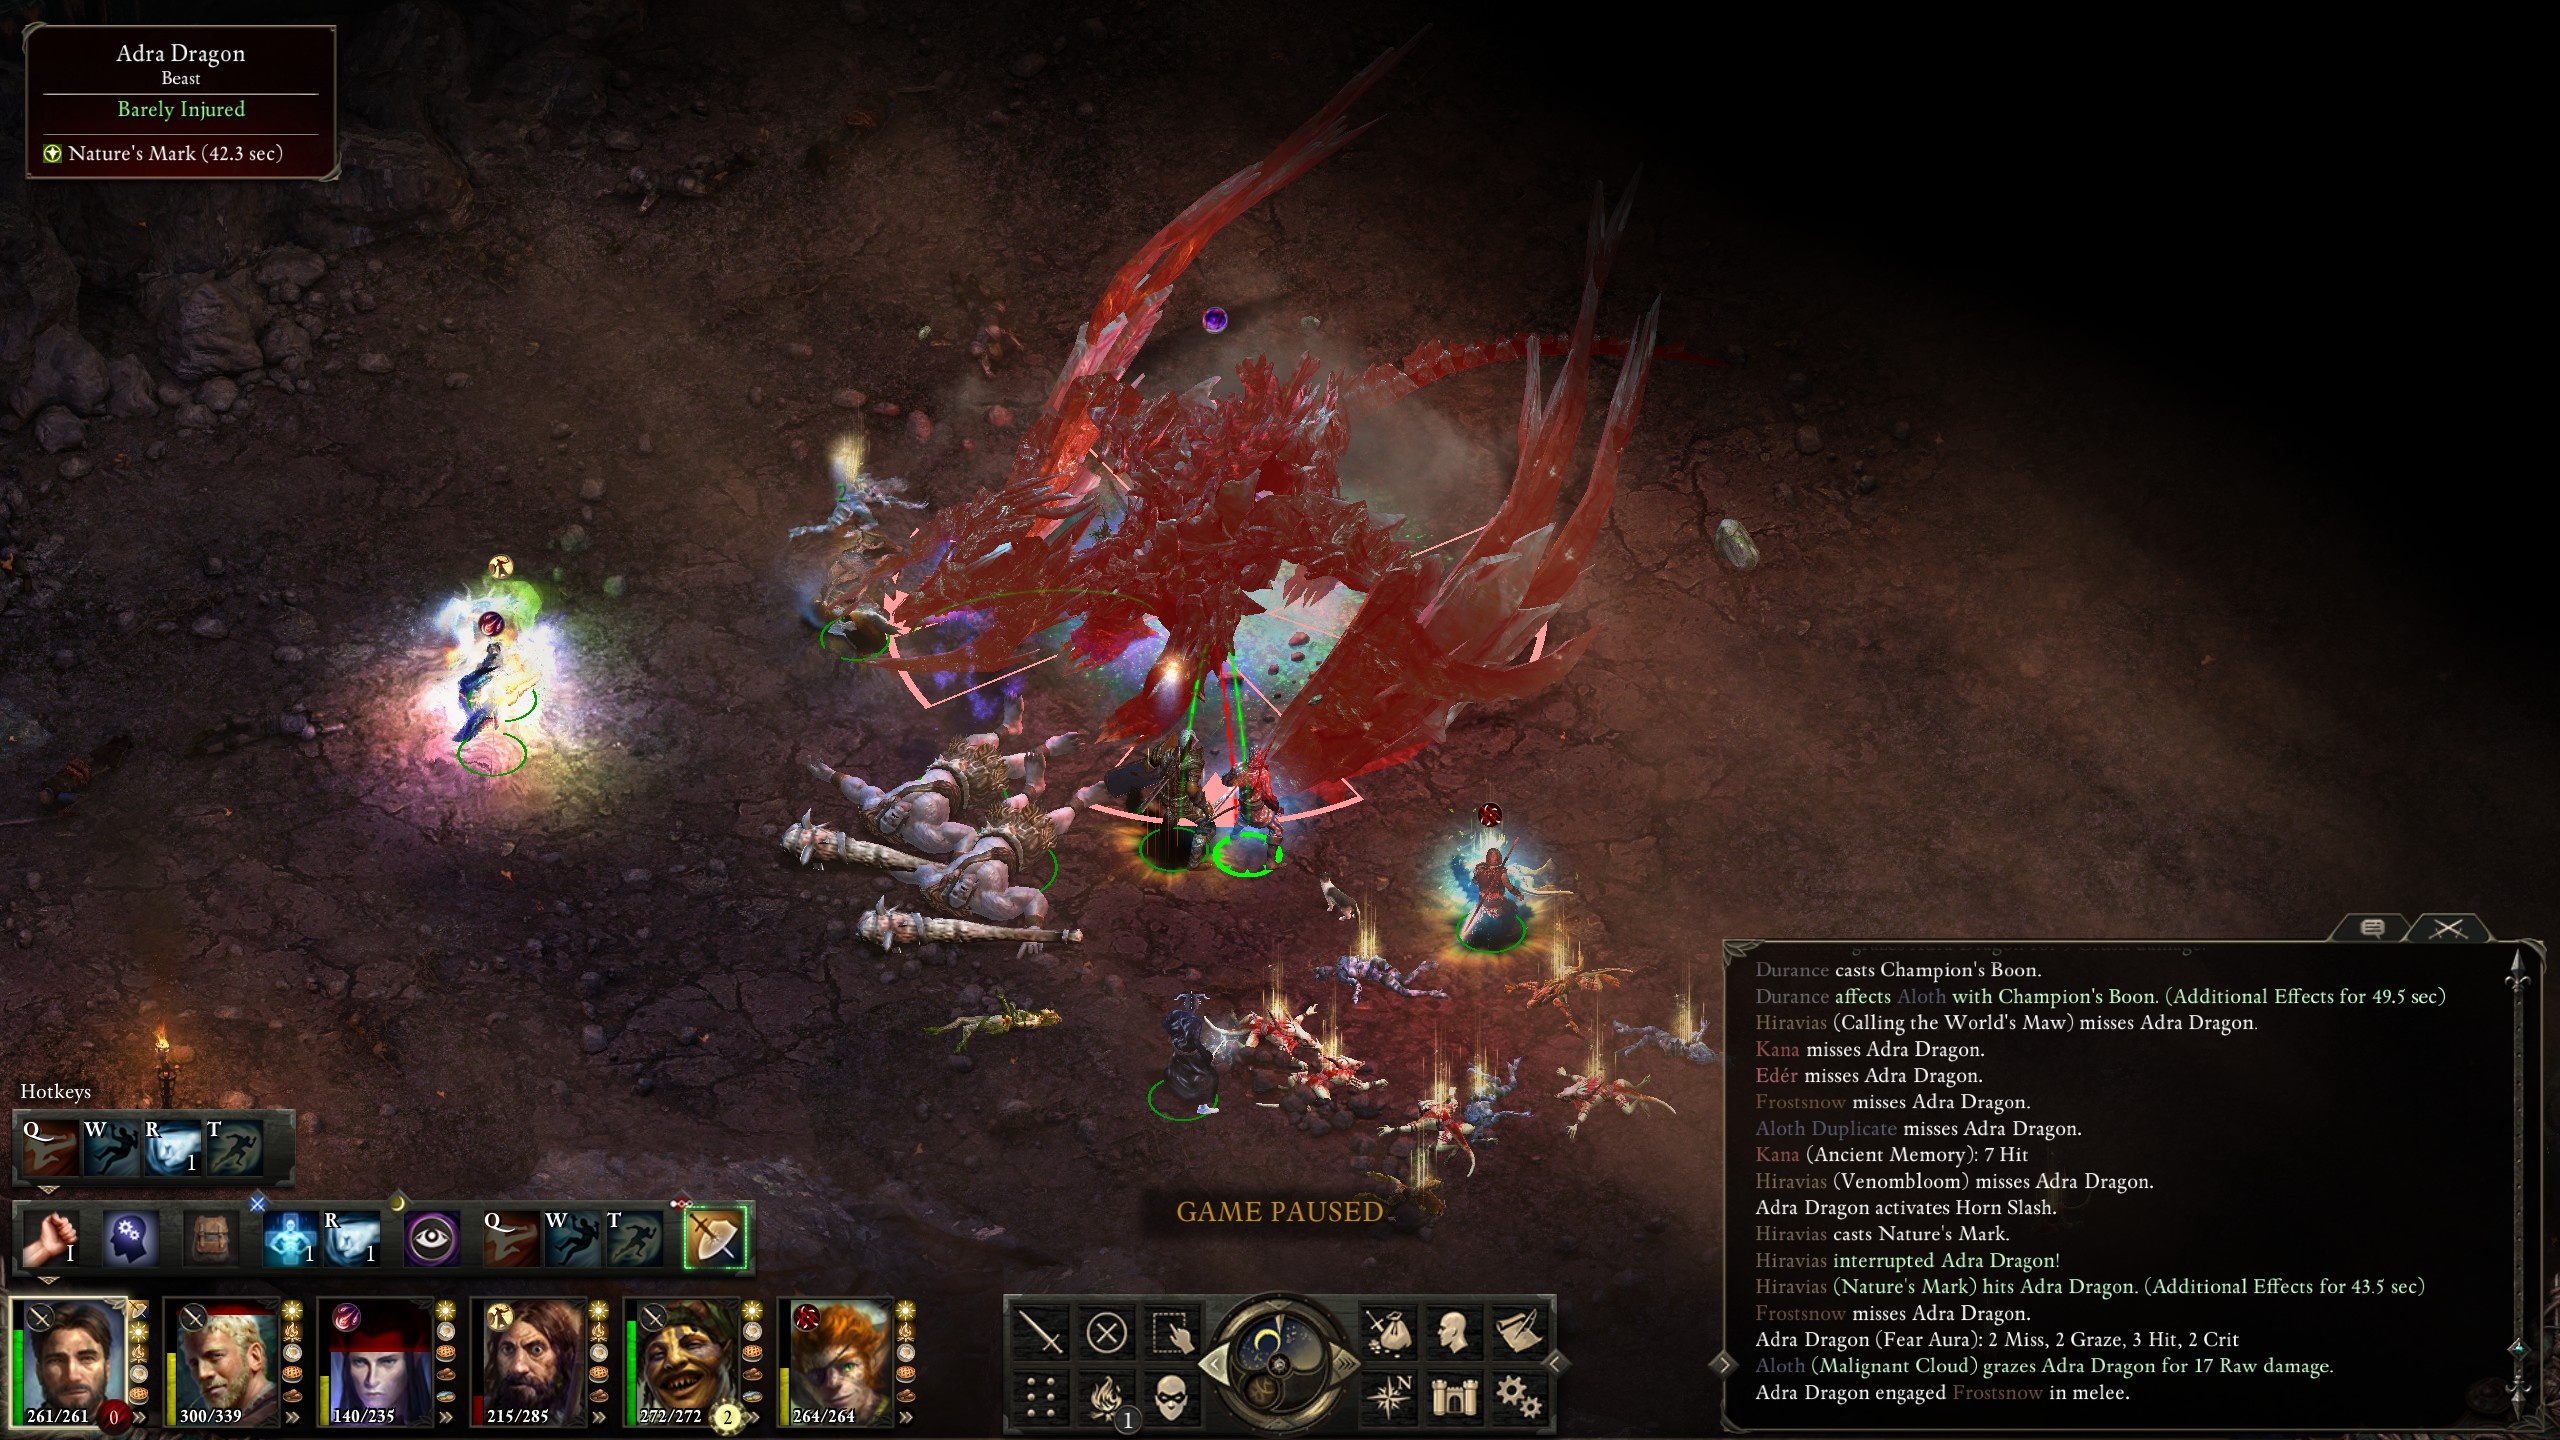
\includegraphics[scale=0.33]{files/blog/2019_03_17_pillars_of_eternity_path_of_the_damned_act_iv/2019_03_17_dragon2_09.jpg}
\end{figure}

For its next moves the dragon decided to throw a Wing Slam to the west followed by a Breath attack to the south.  As I had anticipated, each group was able to to survive the attack, although they had some serious healing to do before the next attacks.

\begin{figure}
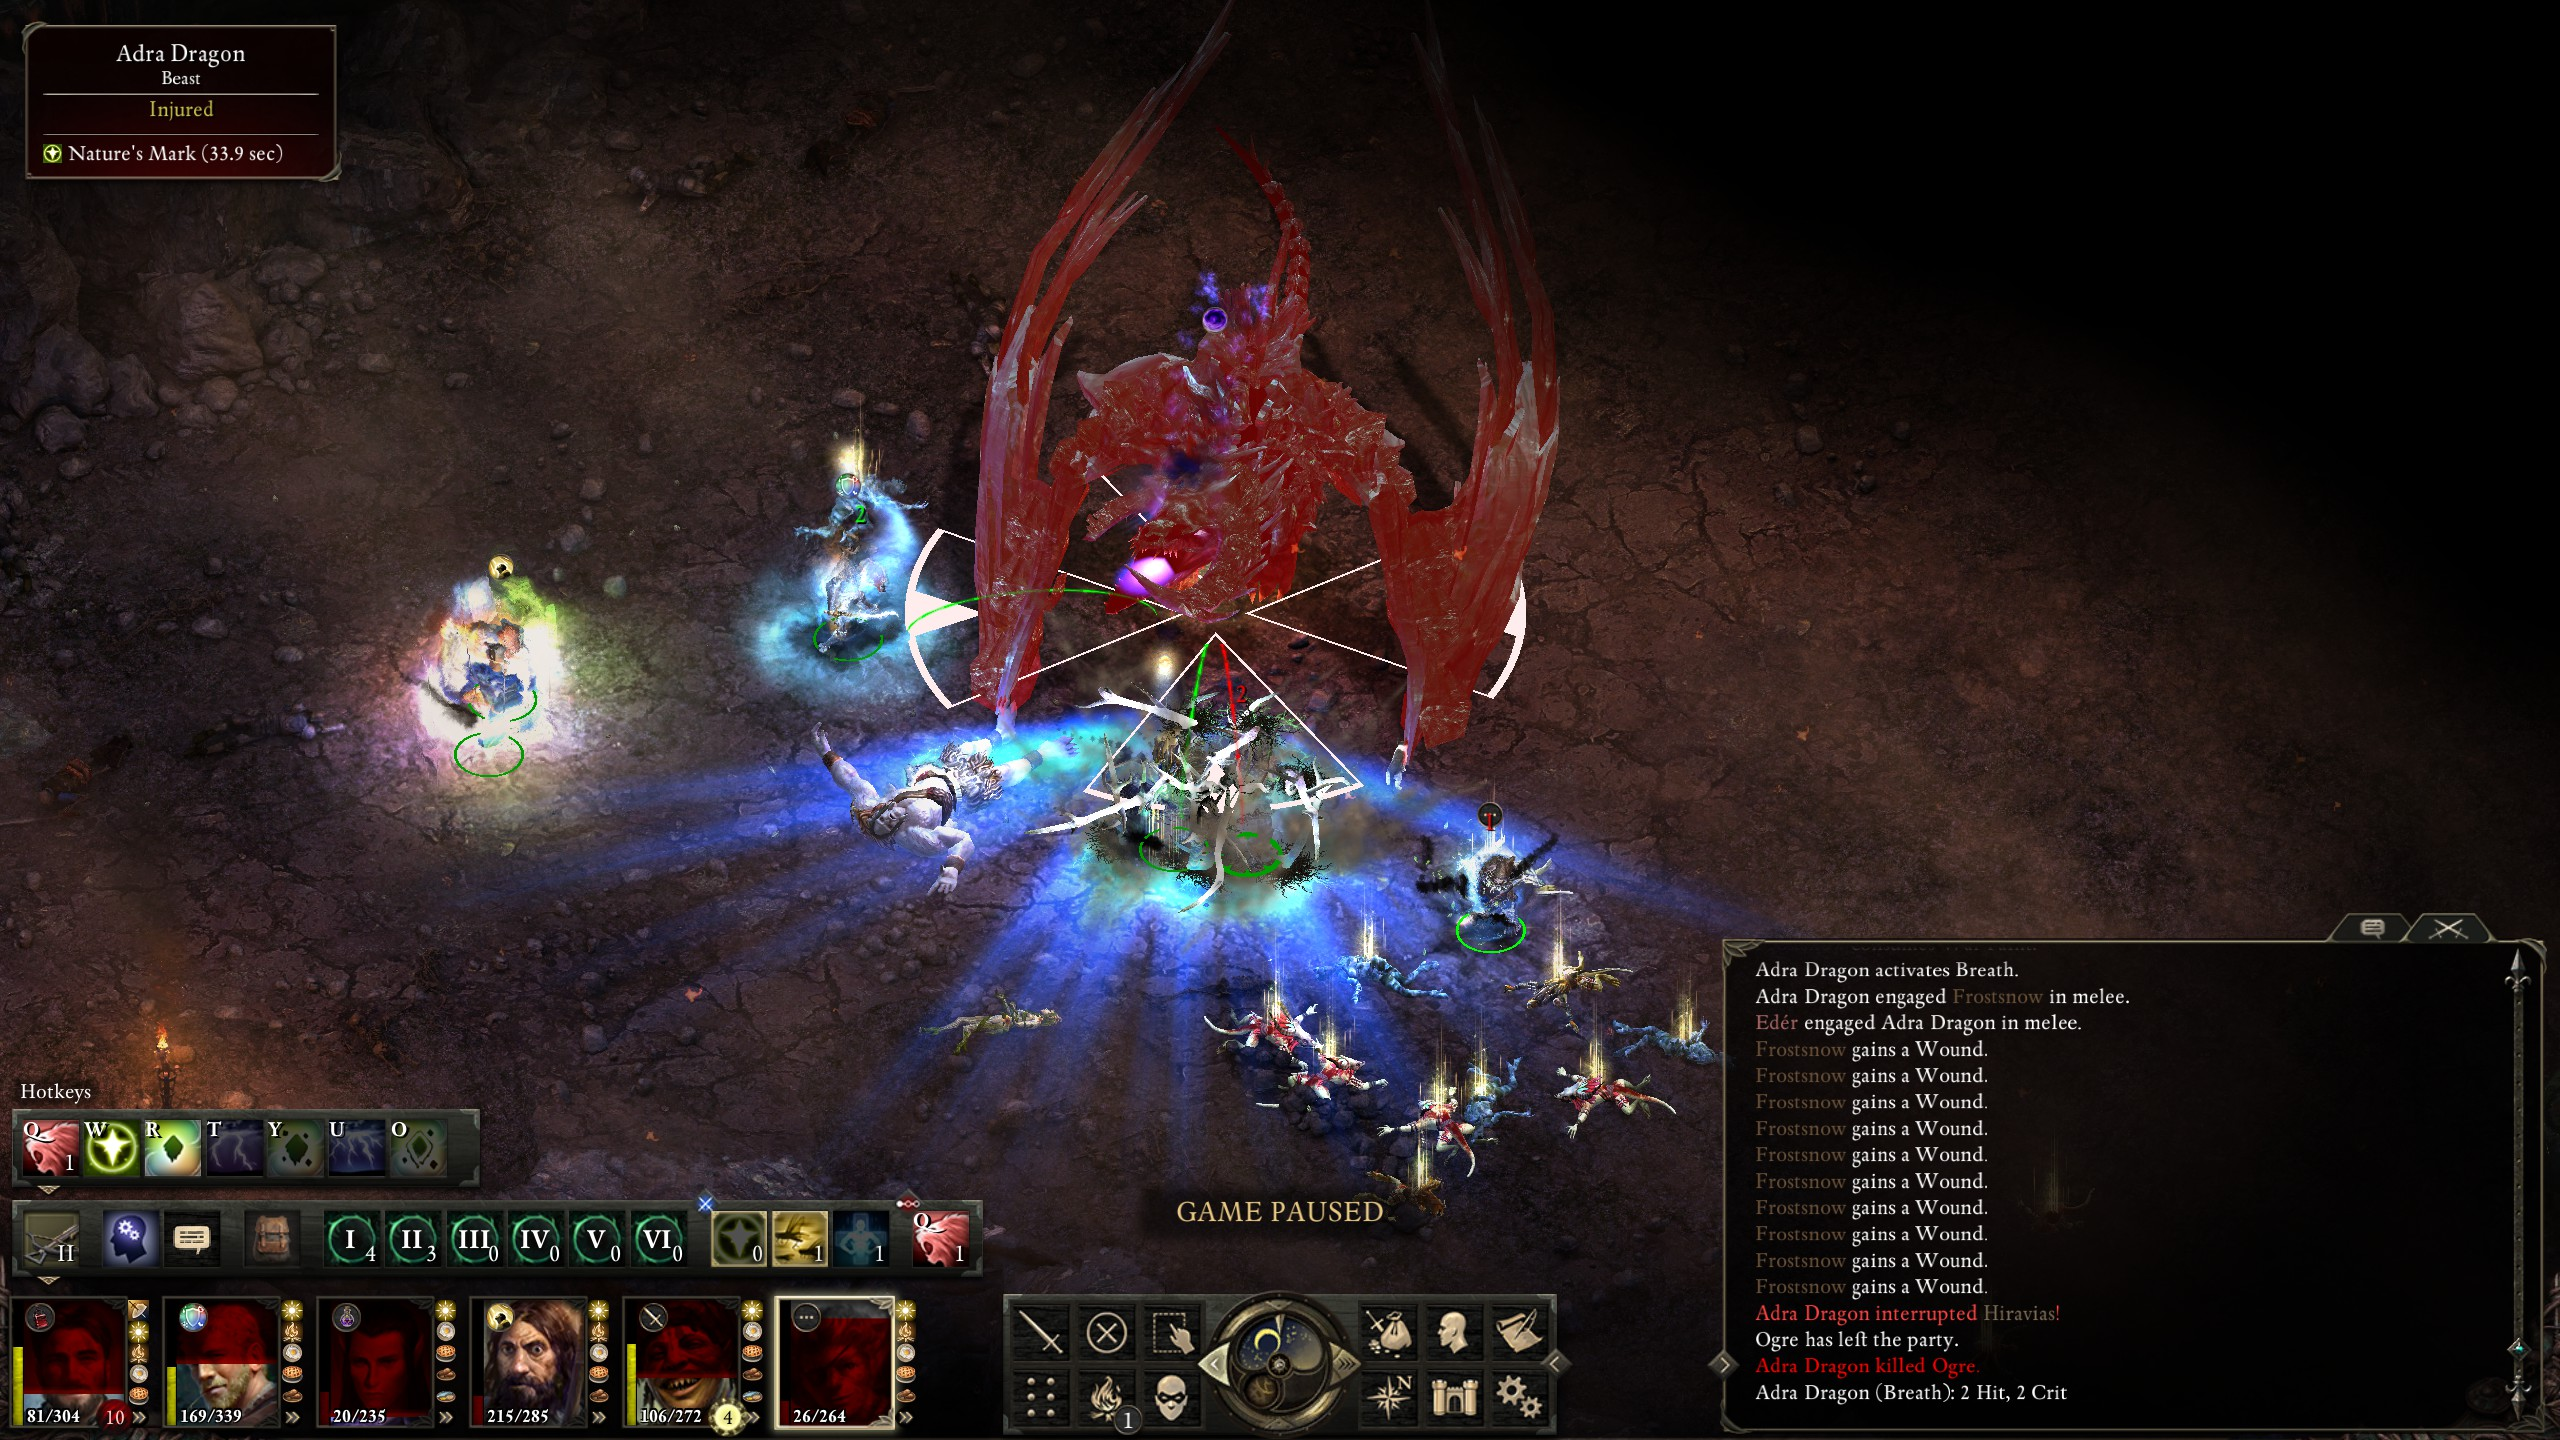
\includegraphics[scale=0.33]{files/blog/2019_03_17_pillars_of_eternity_path_of_the_damned_act_iv/2019_03_17_dragon2_10.jpg}
\end{figure}

In fact, Hiravas was low enough that it was time to have Durance cast "Barring Death's Door" on him, so I had him move away from the dragon until the spell had cast.

\begin{figure}
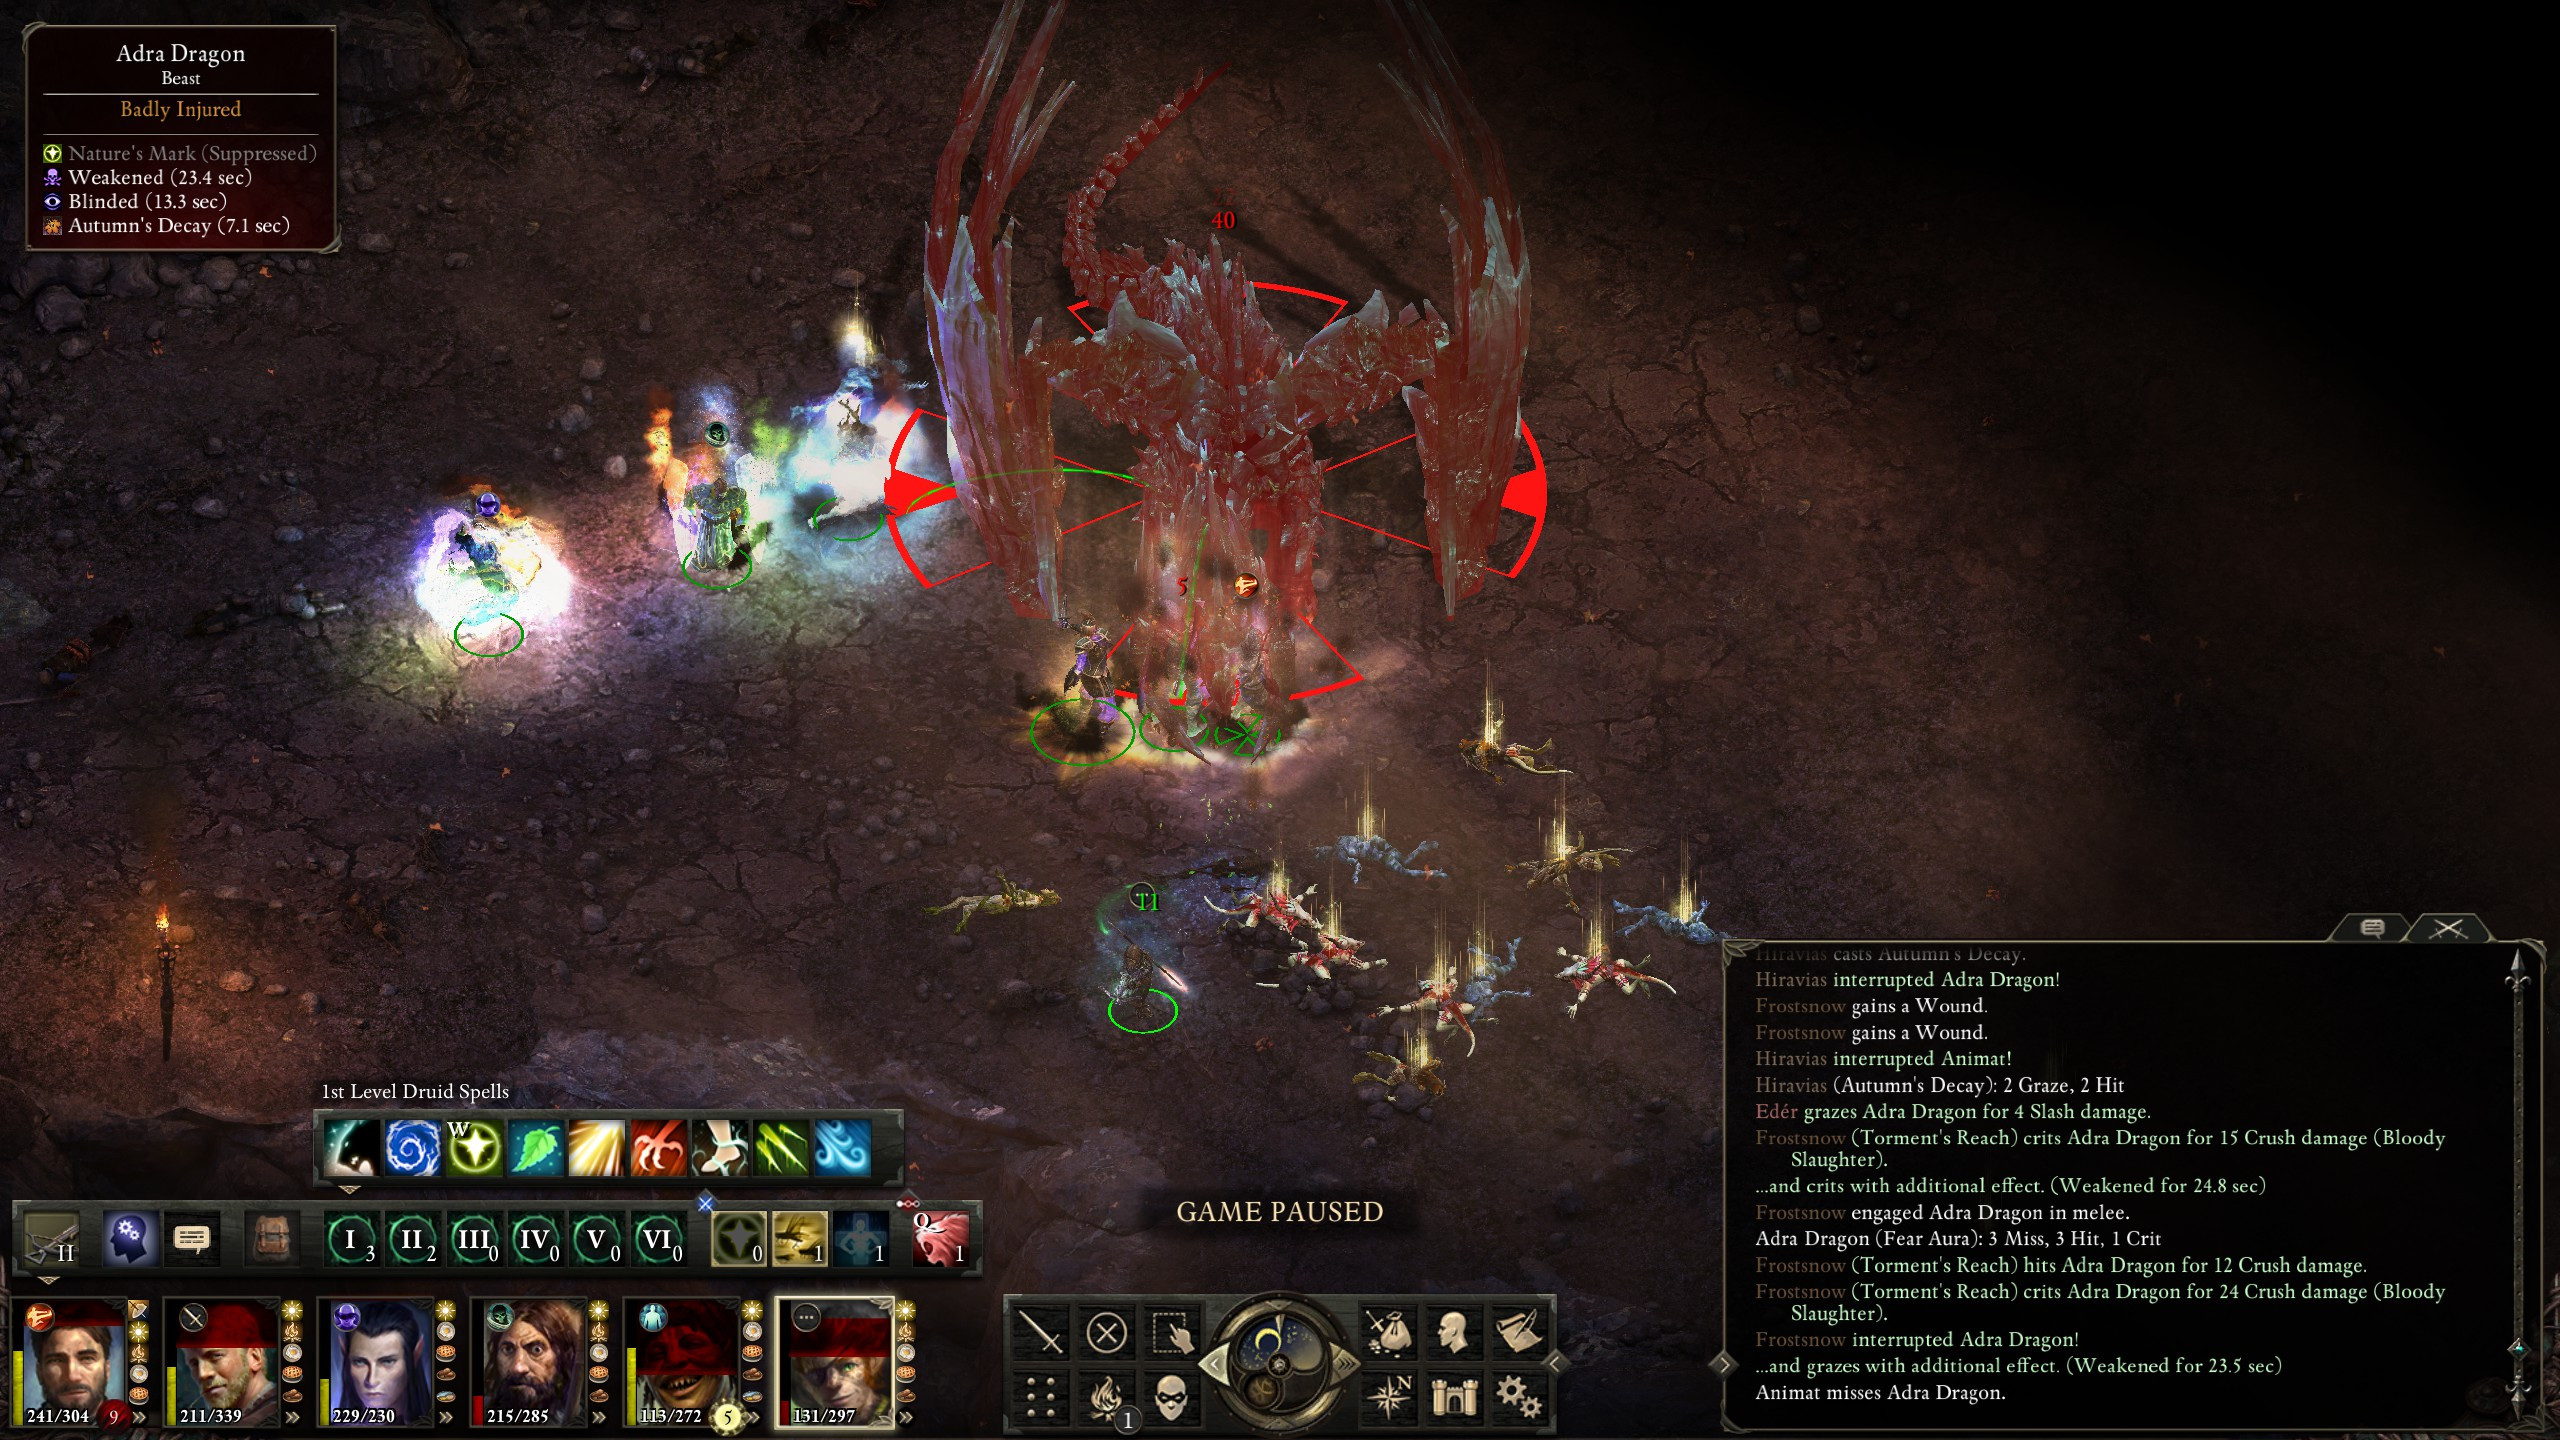
\includegraphics[scale=0.33]{files/blog/2019_03_17_pillars_of_eternity_path_of_the_damned_act_iv/2019_03_17_dragon2_11.jpg}
\end{figure}

This turned out to be a great idea, because the dragon soon after decided to use its Wing Slam, and I was able to maneuver Hiravas out of its range.

\begin{figure}
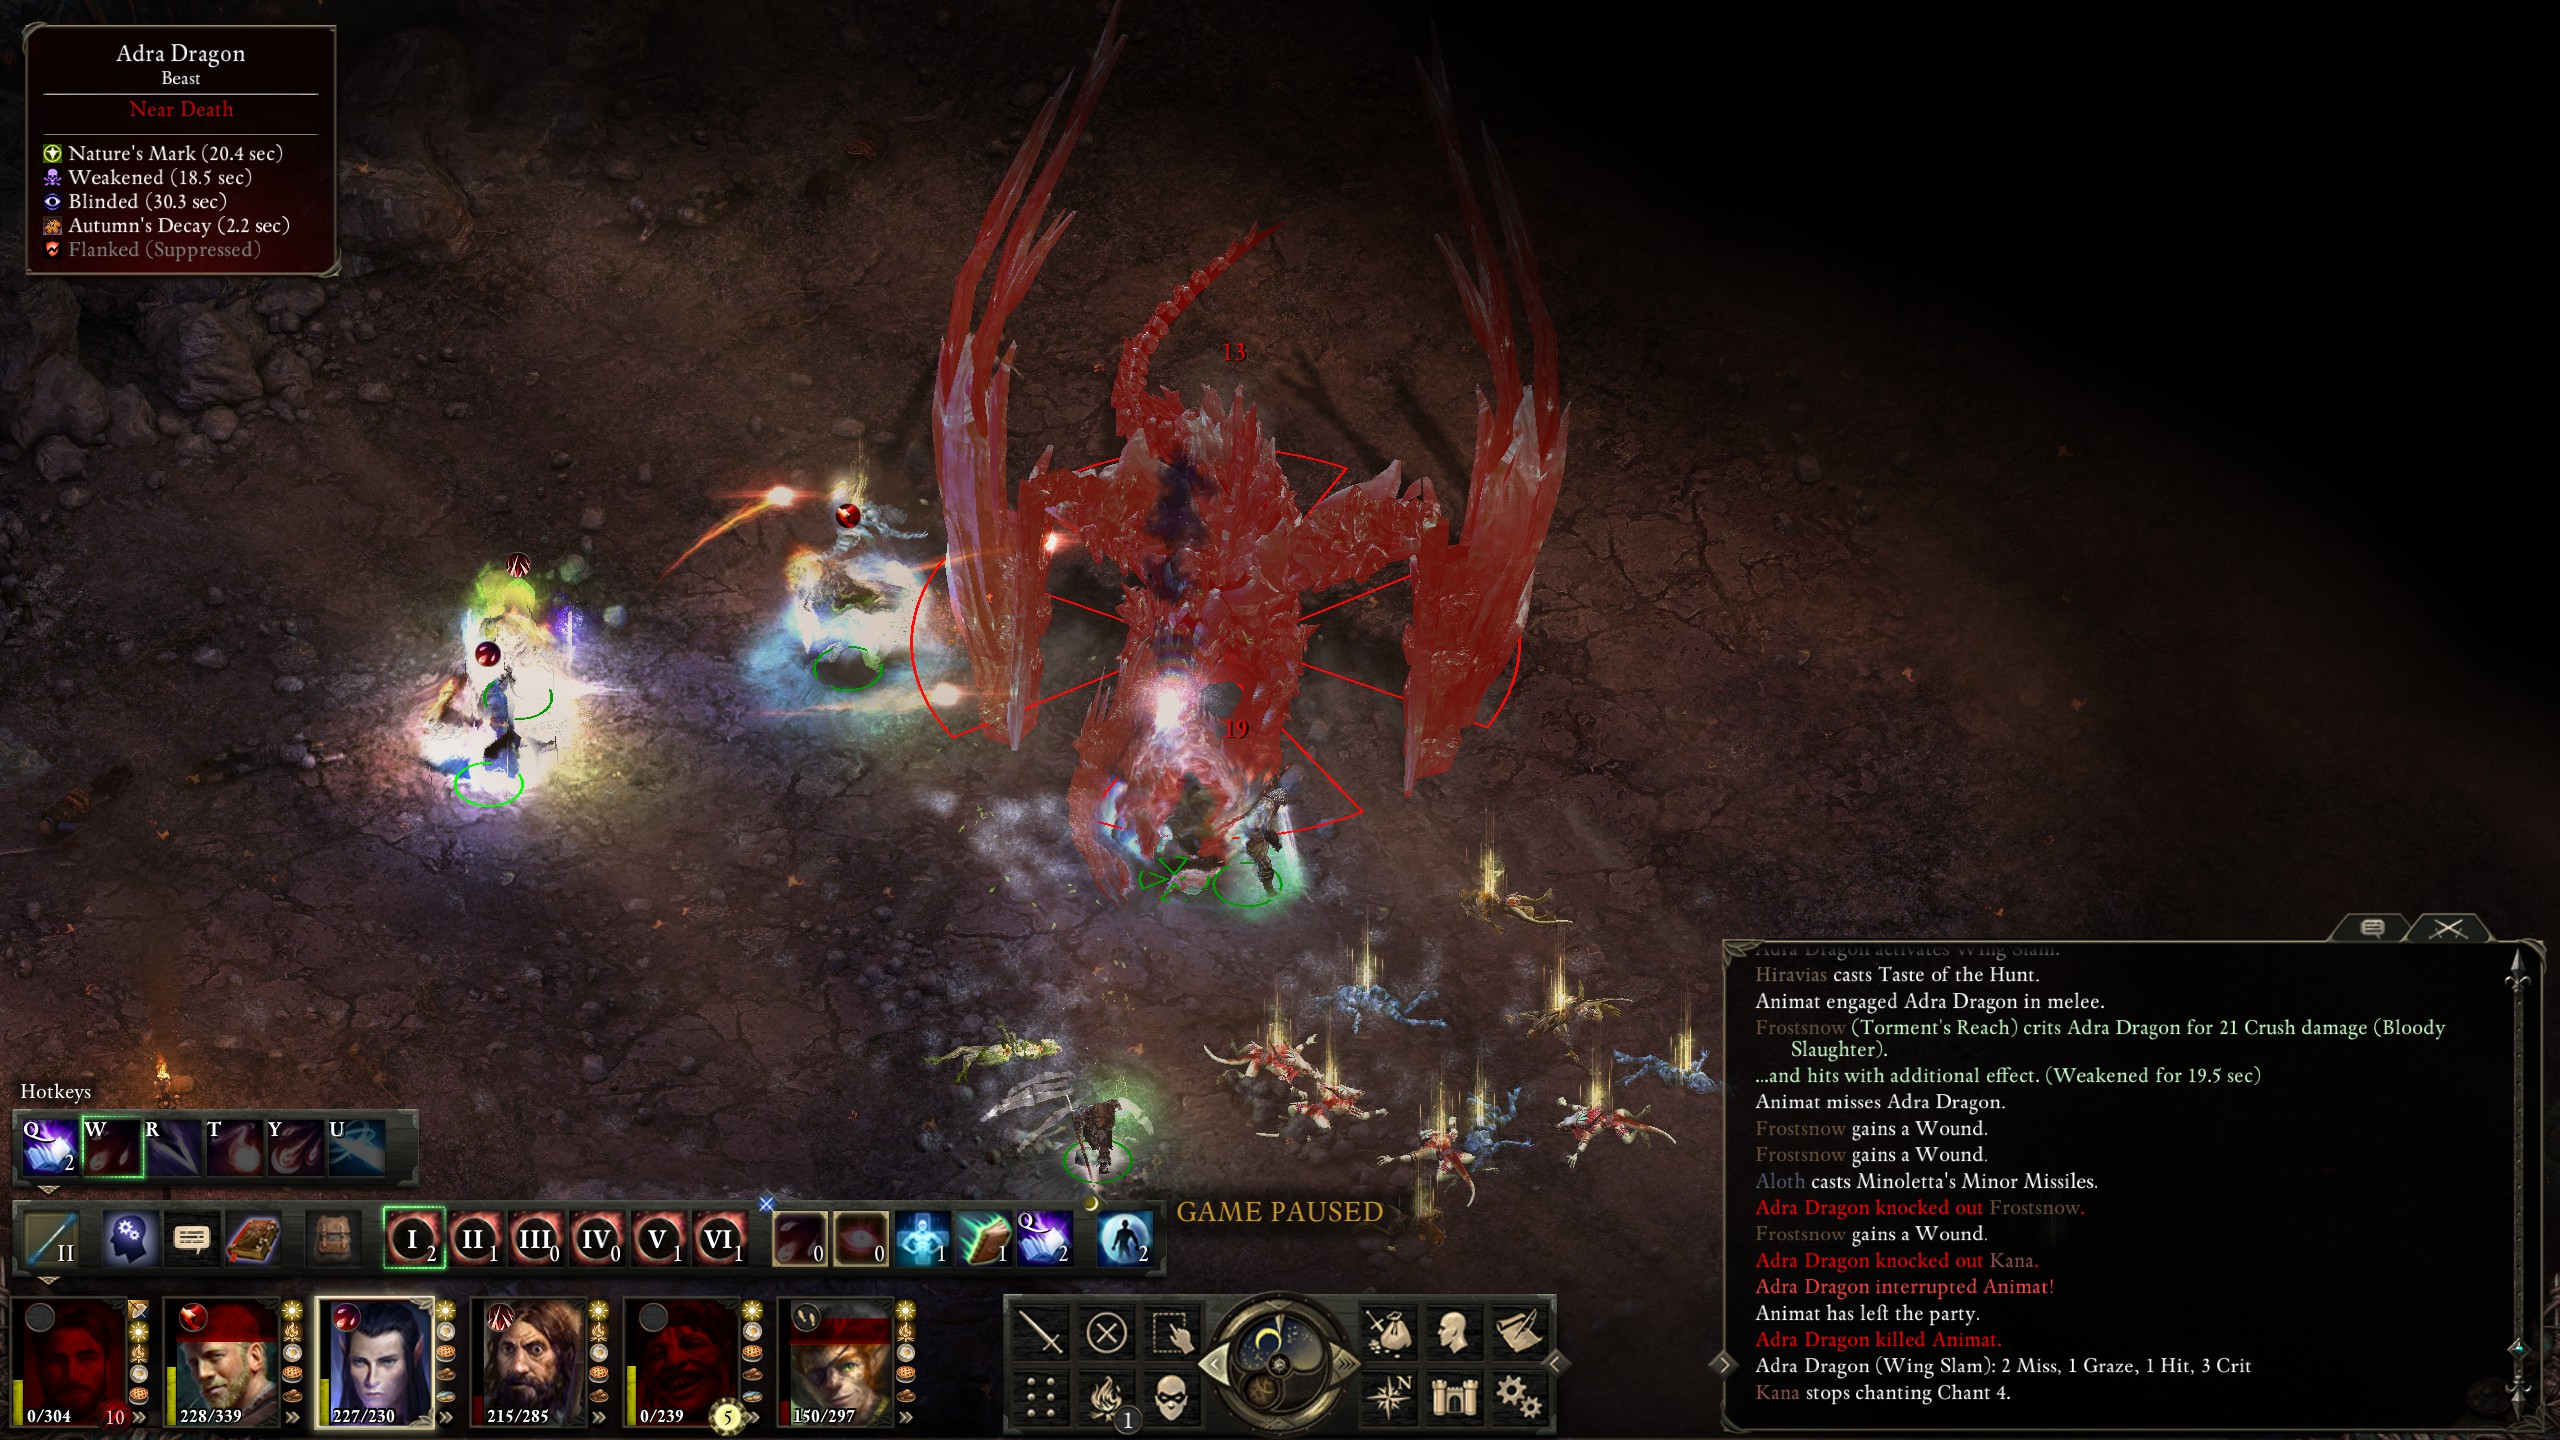
\includegraphics[scale=0.33]{files/blog/2019_03_17_pillars_of_eternity_path_of_the_damned_act_iv/2019_03_17_dragon2_12.jpg}
\end{figure}

Since I'd giving Hiravas the "Remembrance Ashes" I then had him revive Kana, who then proceeded to use "Rise Again, Rise Again, Scions of Adon!" to revive my monk.

\begin{figure}
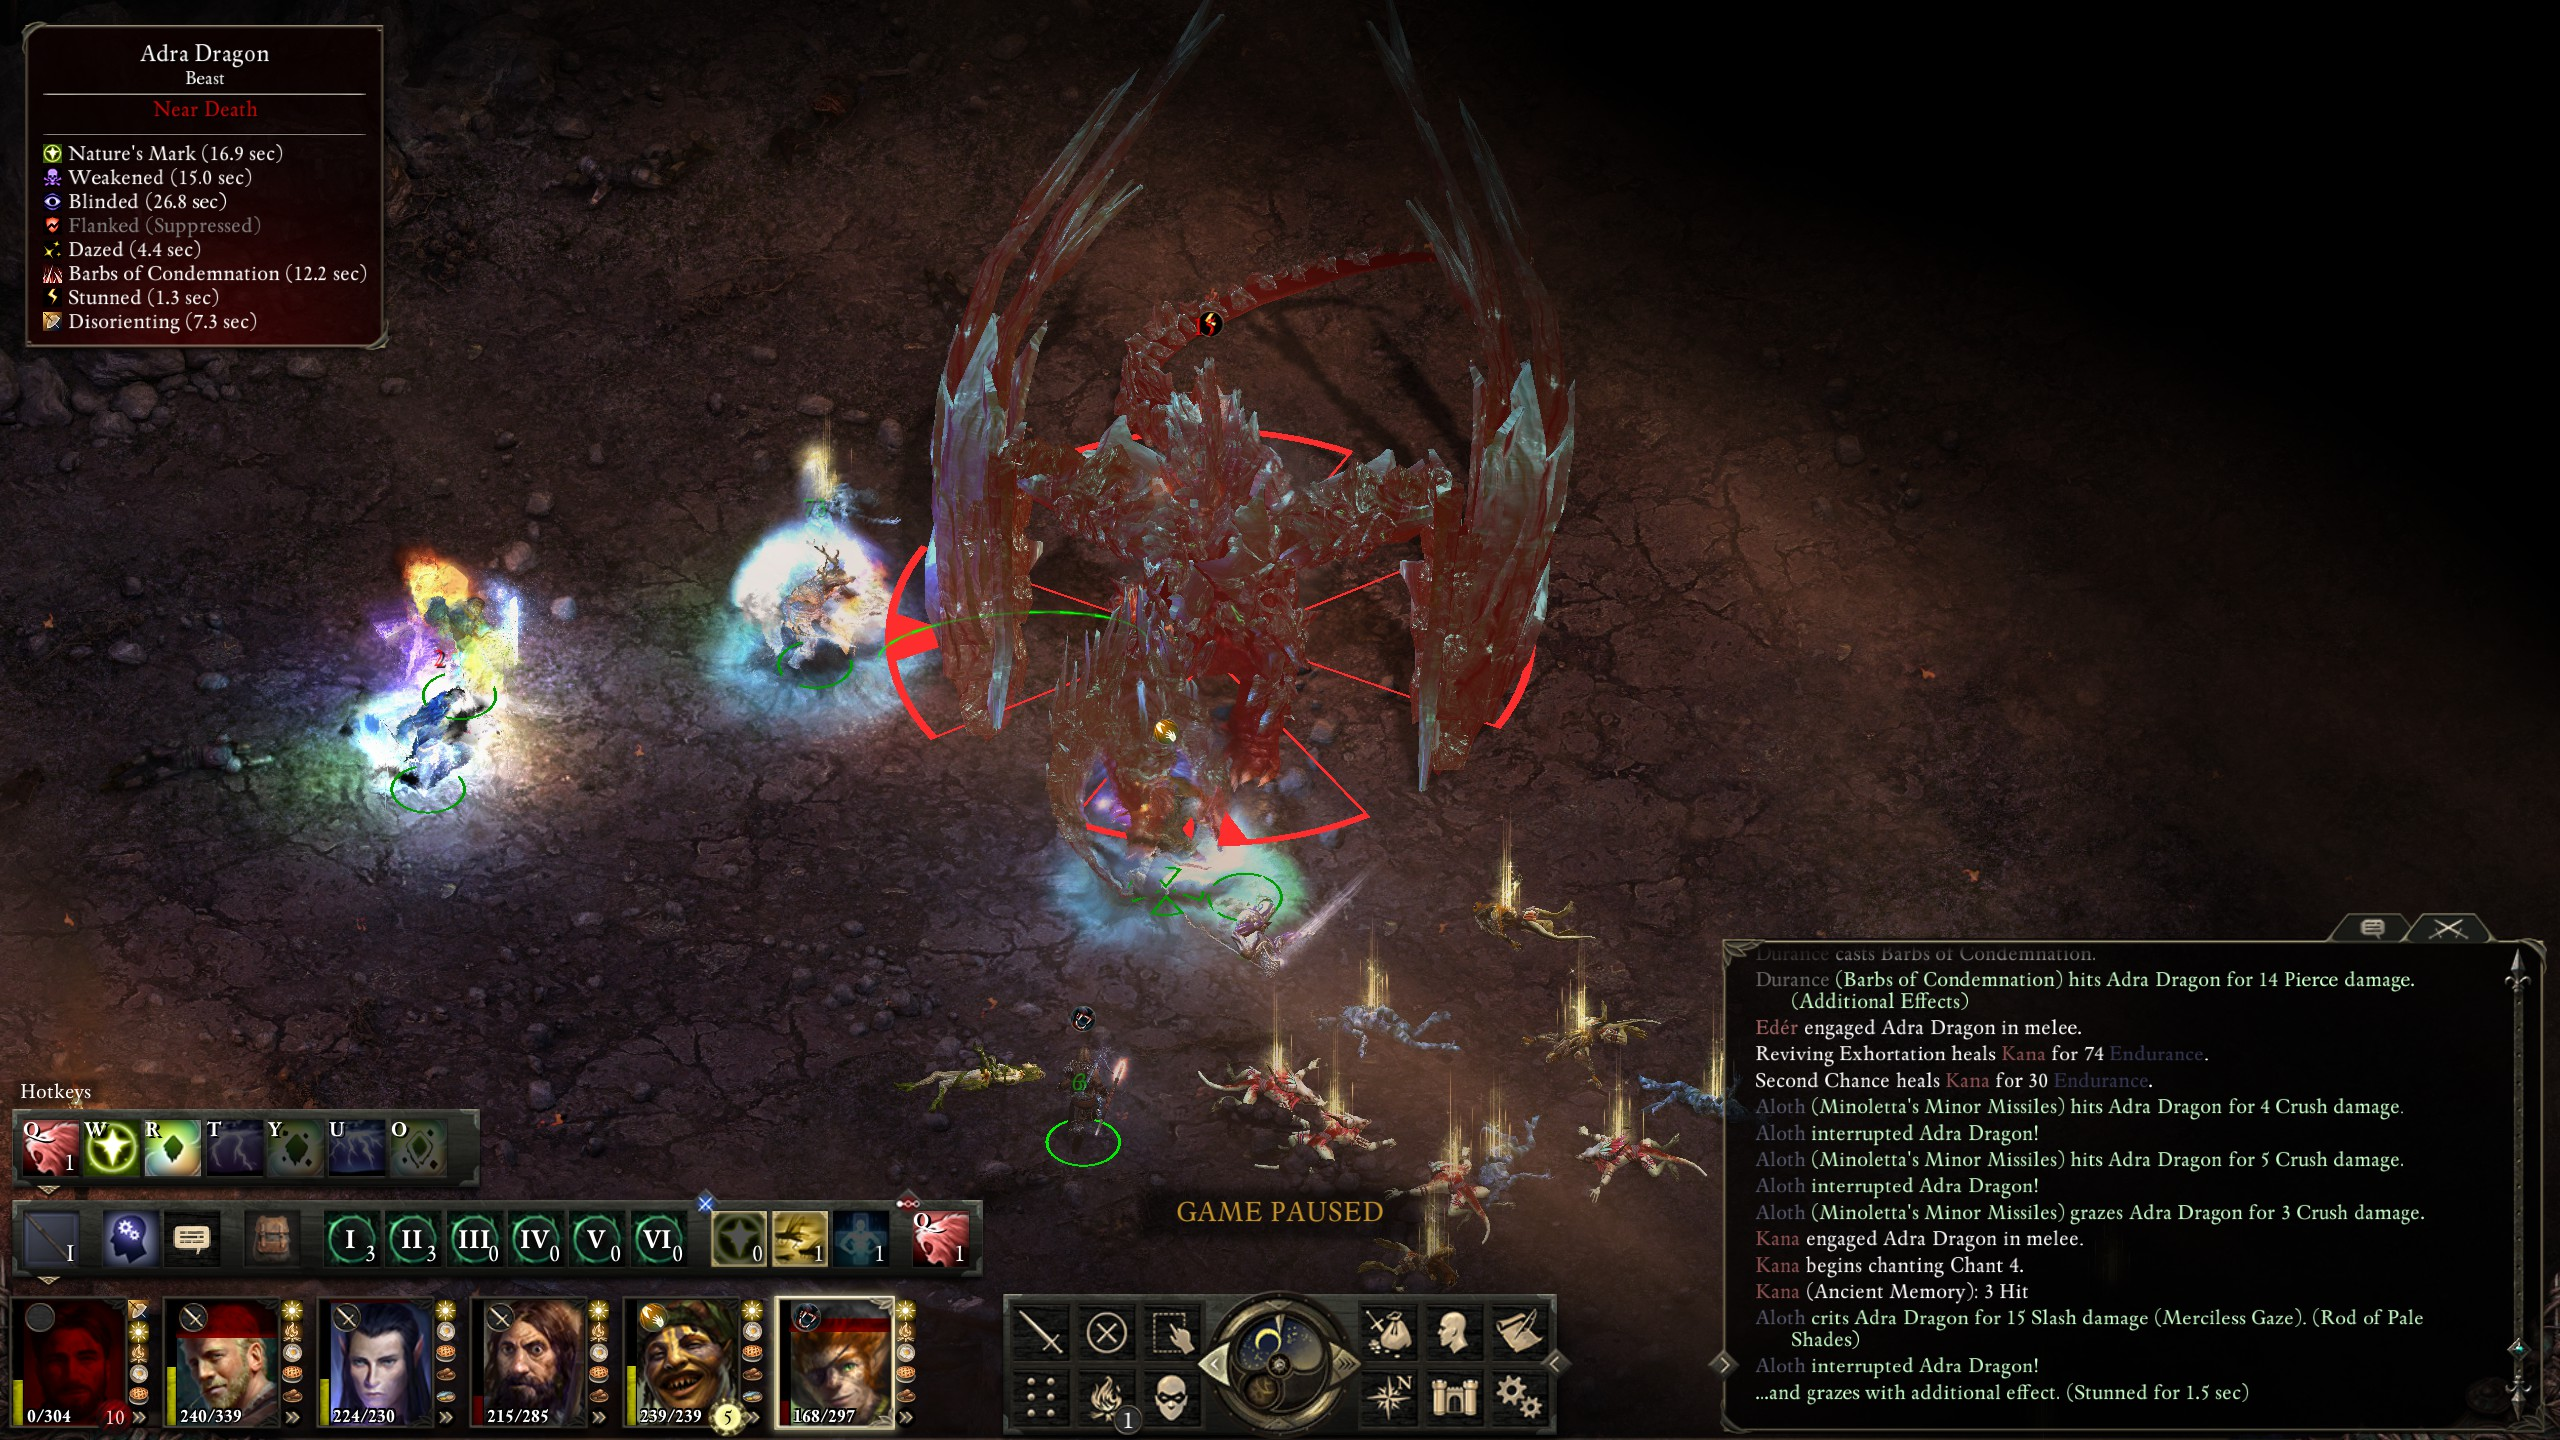
\includegraphics[scale=0.33]{files/blog/2019_03_17_pillars_of_eternity_path_of_the_damned_act_iv/2019_03_17_dragon2_13.jpg}
\end{figure}

Before he could do that, though, the brave tank Eder landed the killing blow with a whopping 5 damage (thanks in part to the stun Aloth landed from his wand)!

\begin{figure}
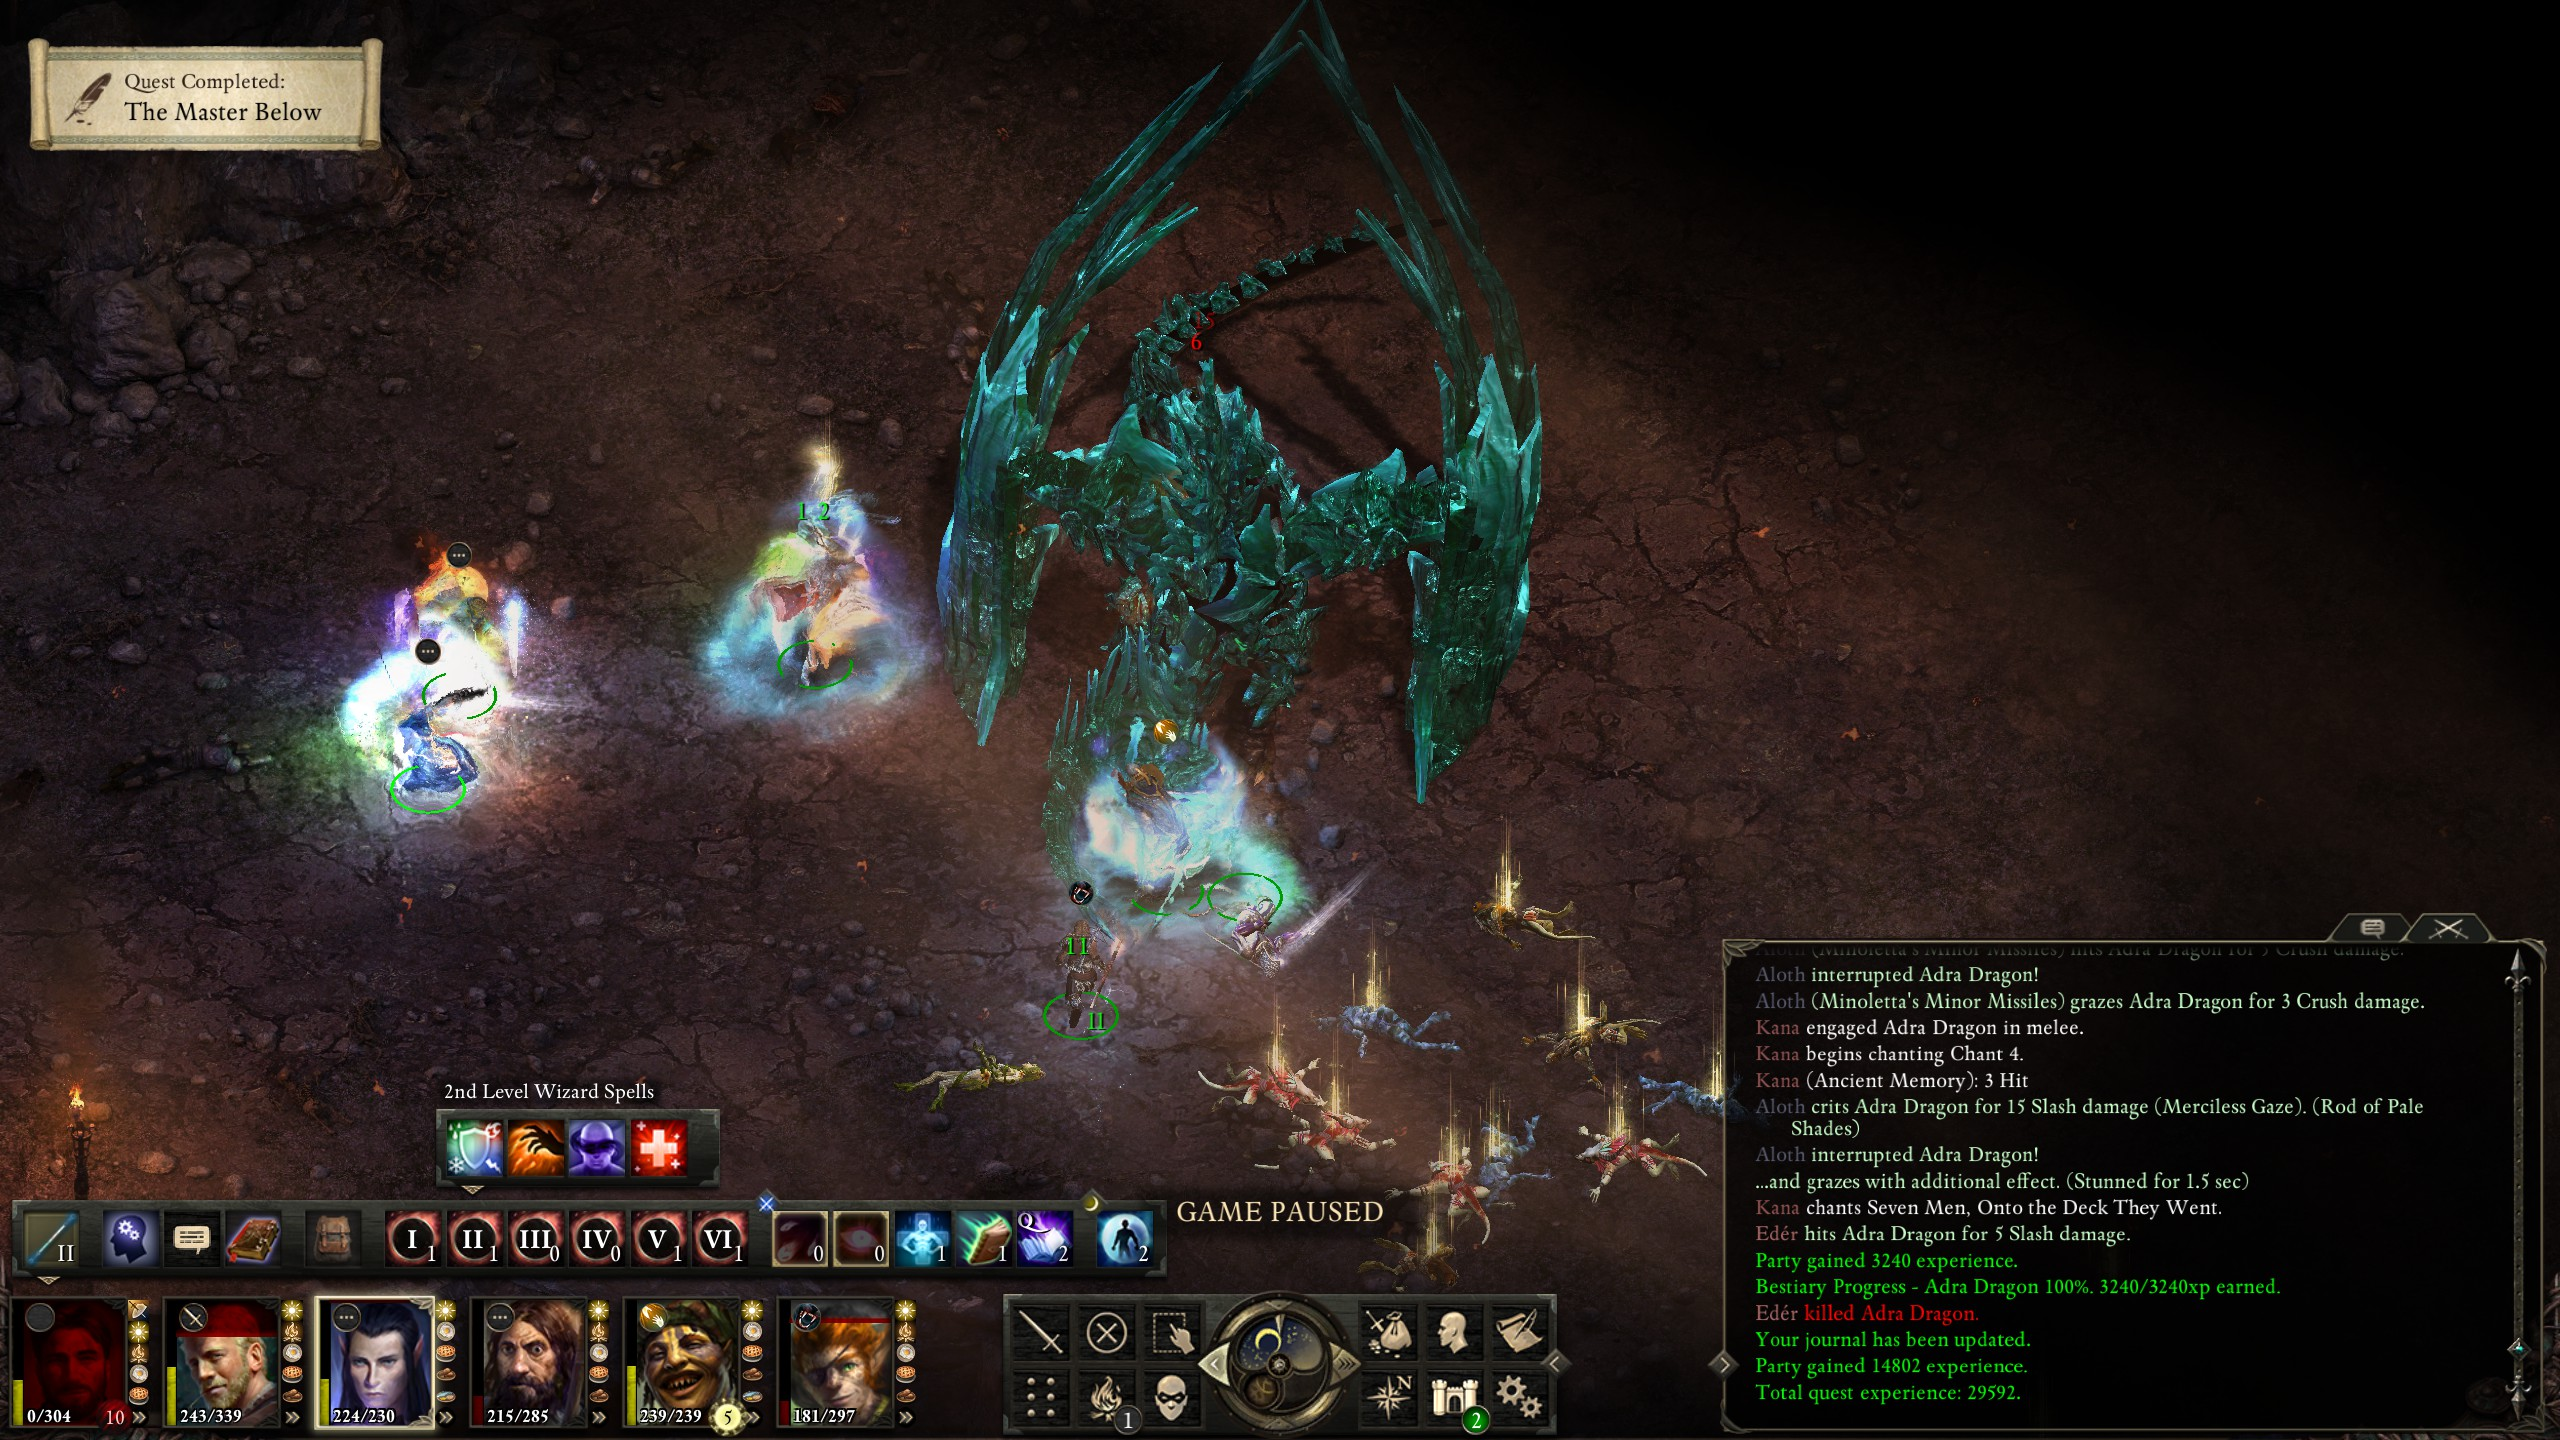
\includegraphics[scale=0.33]{files/blog/2019_03_17_pillars_of_eternity_path_of_the_damned_act_iv/2019_03_17_dragon2_14.jpg}
\end{figure}

Thus the Master Below was defeated, marking an end to one of the most challenging bosses I've ever faced.

\subsection{In Pursuit of Thaos}

With all of the side-quests done and optional bosses dead it was finally time to hunt down Thaos by jumping into the pit.

\begin{figure}
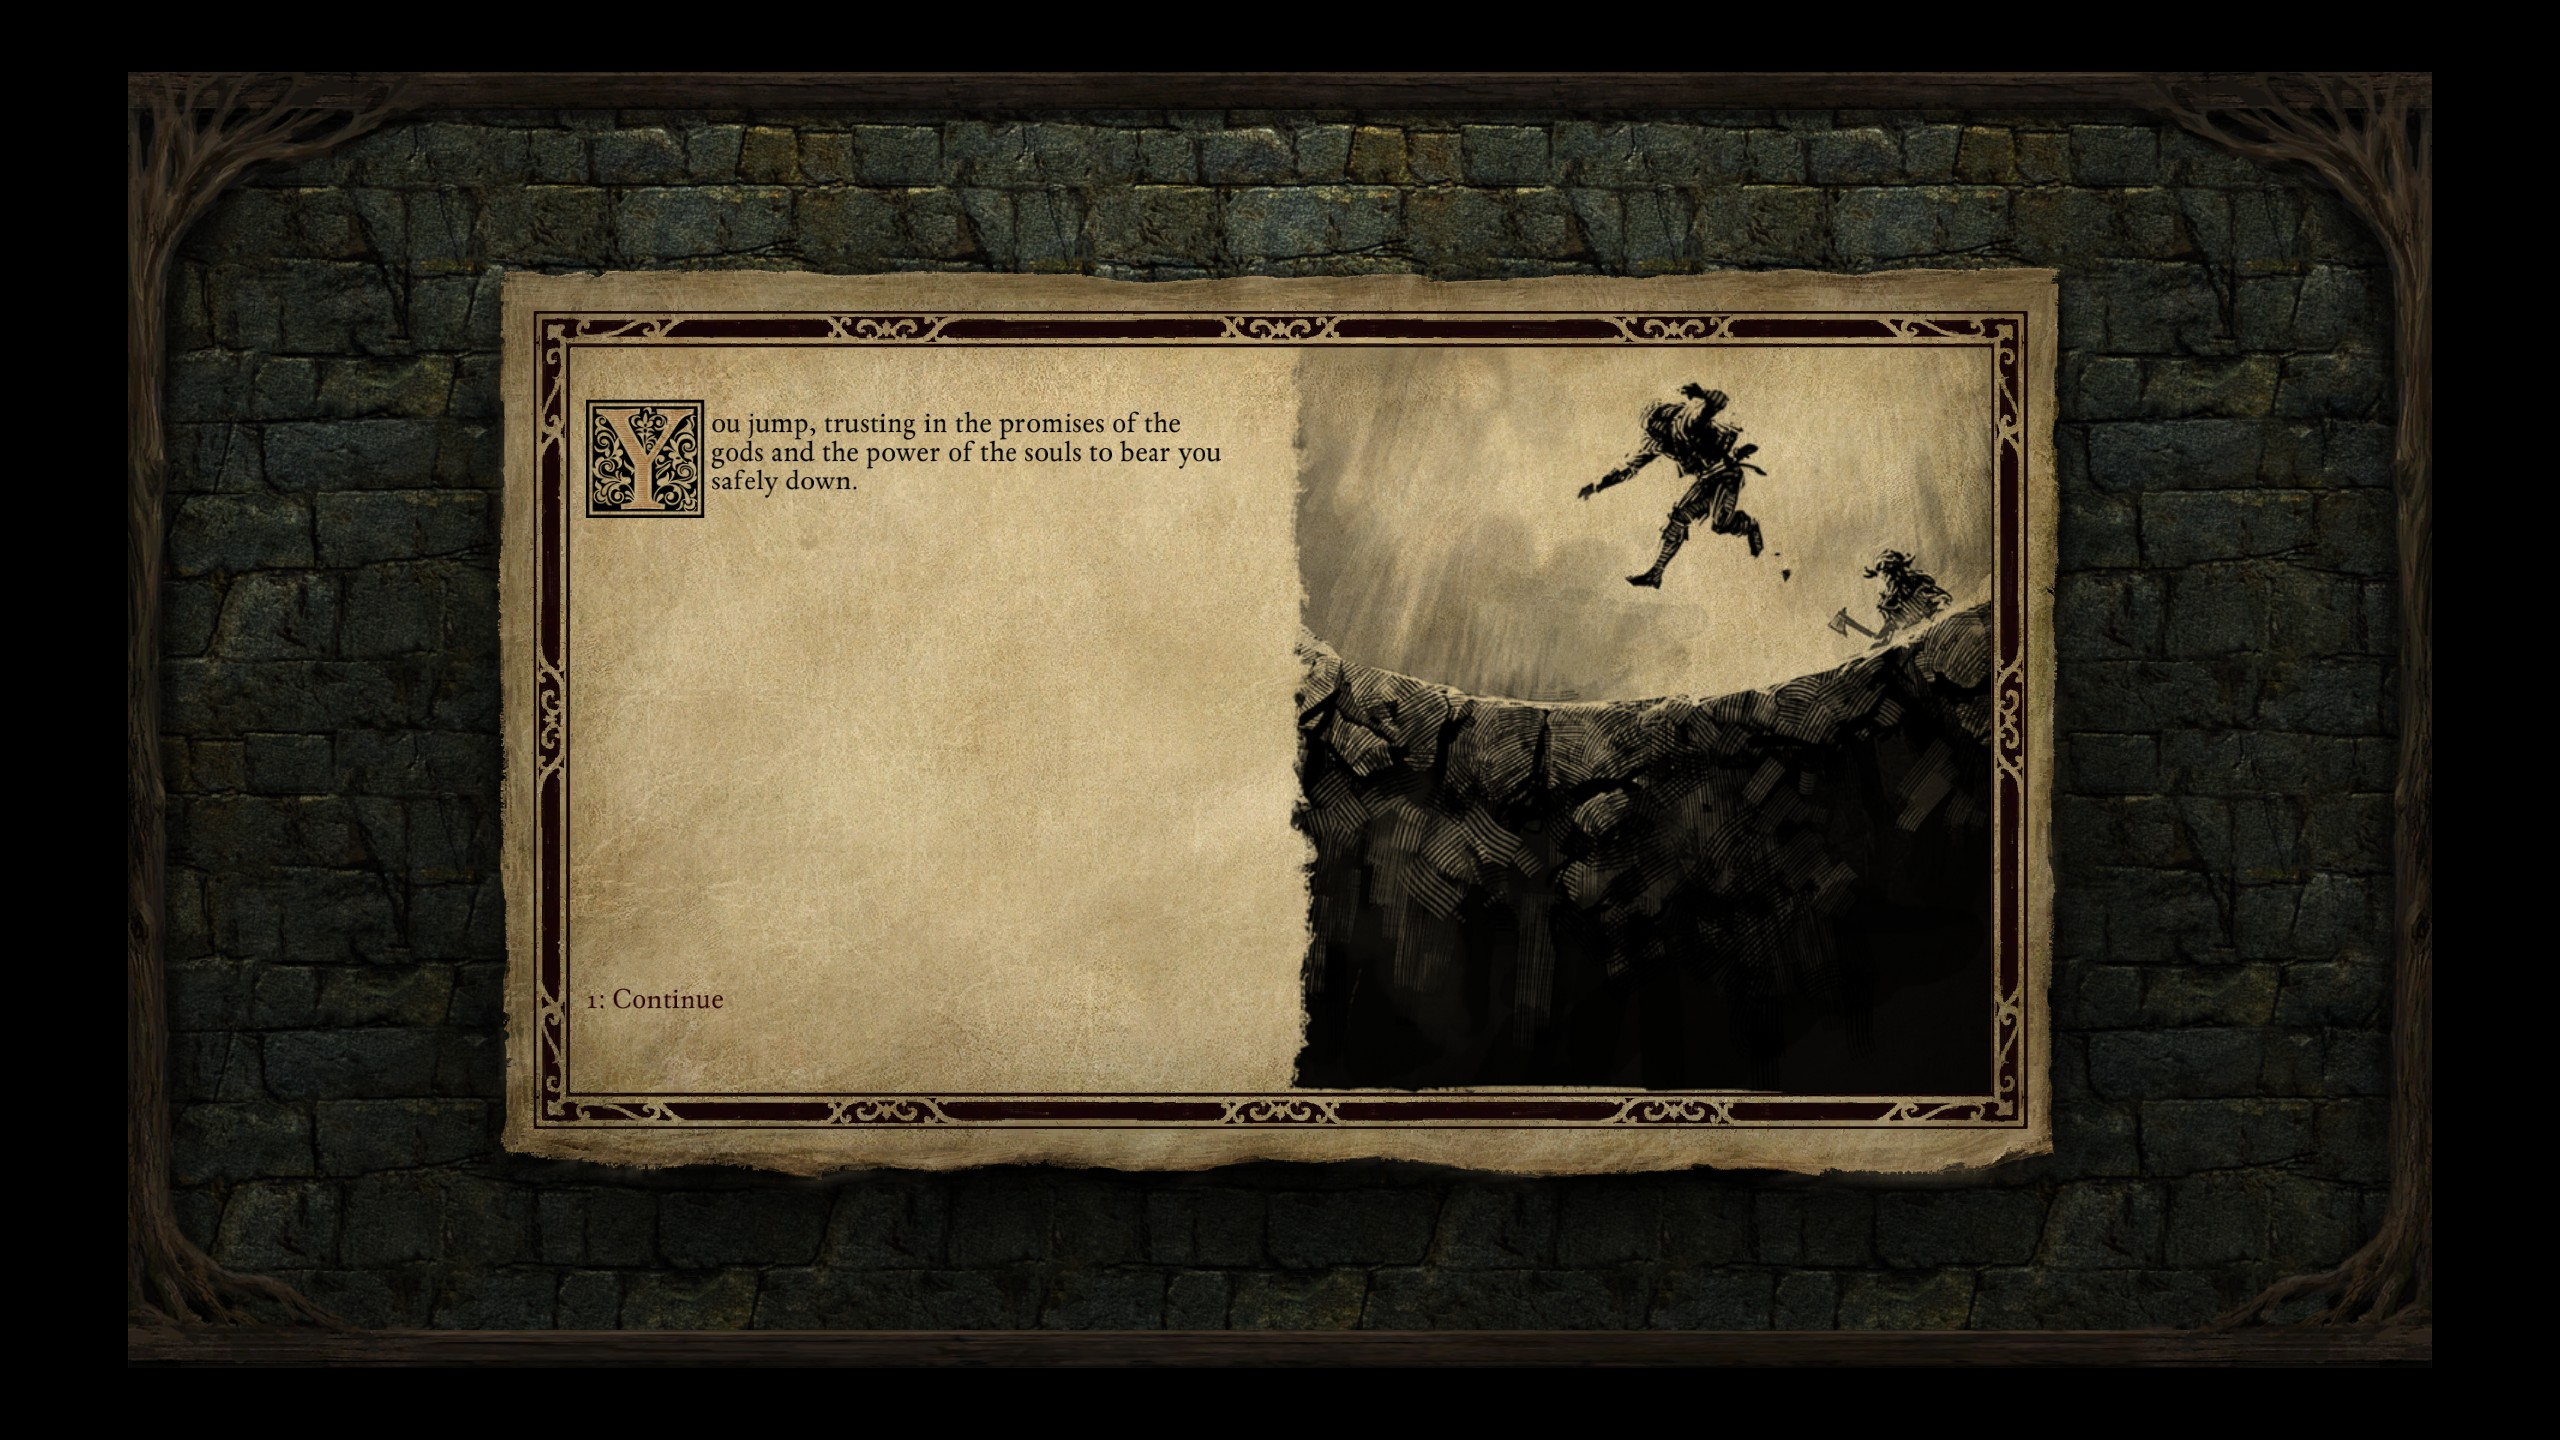
\includegraphics[scale=0.33]{files/blog/2019_03_17_pillars_of_eternity_path_of_the_damned_act_iv/2019_03_17_pit.jpg}
\end{figure}

\subsubsection{Breith Eaman}

\begin{figure}
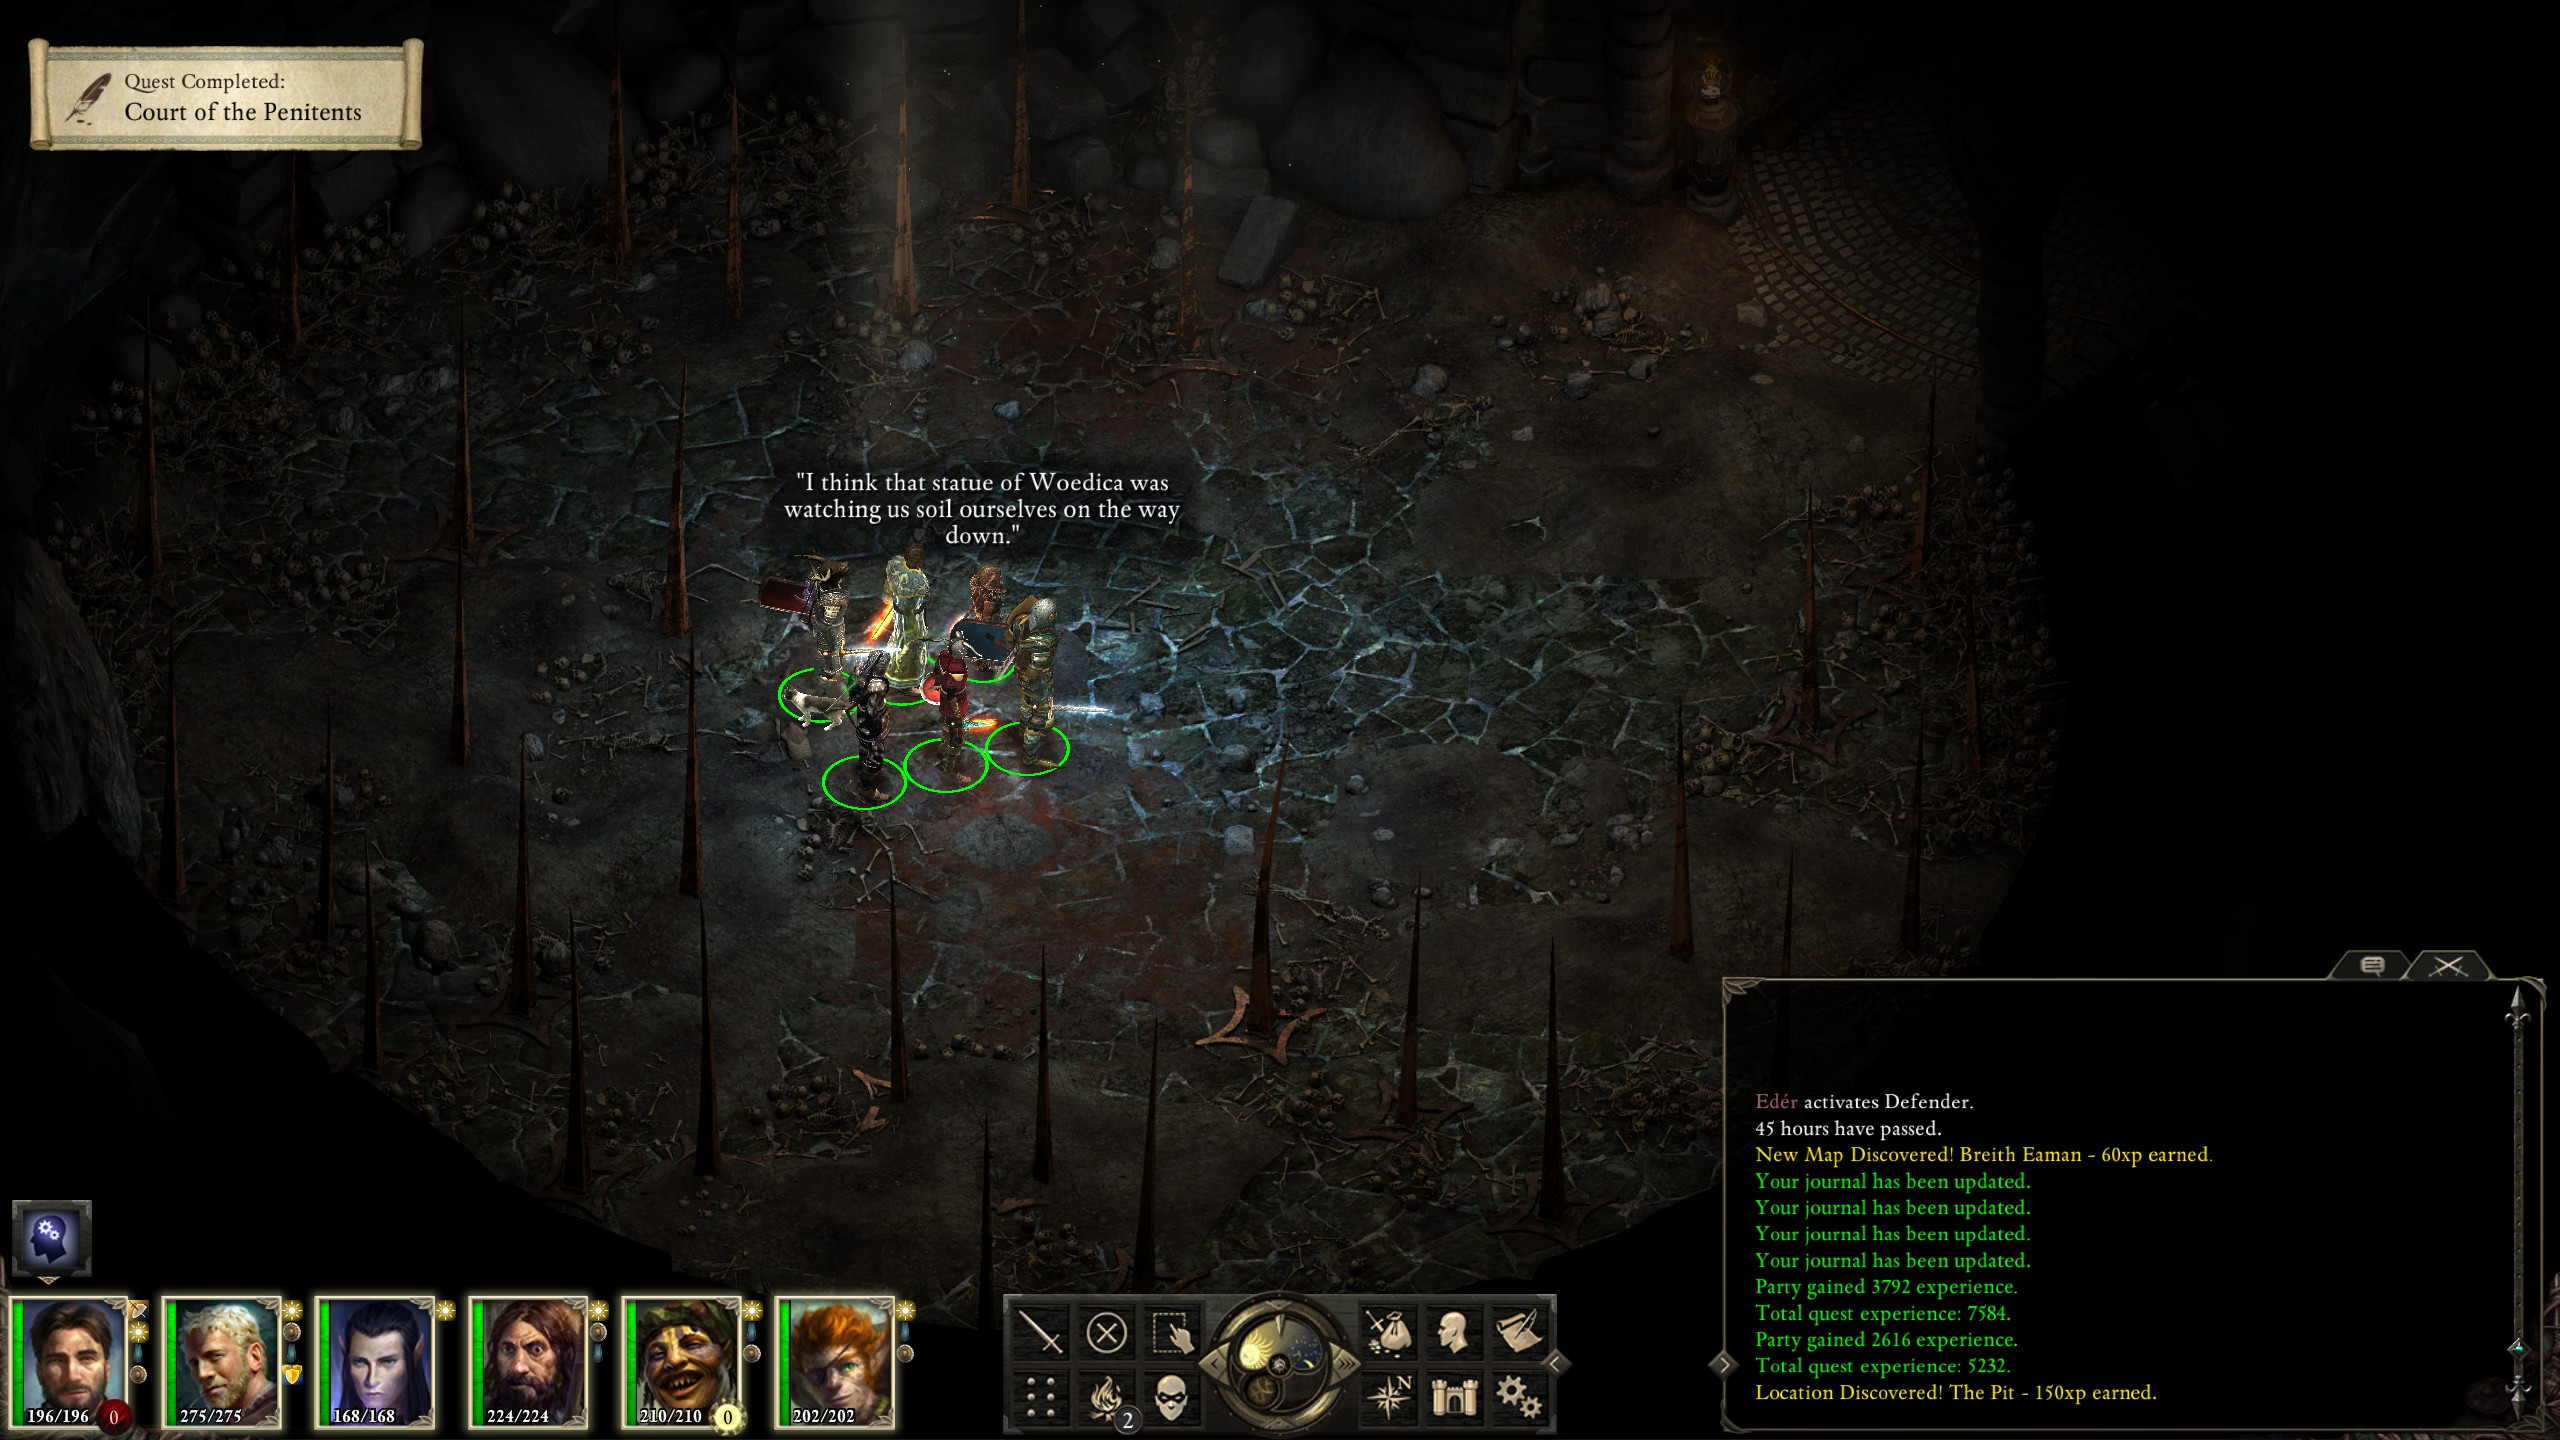
\includegraphics[scale=0.33]{files/blog/2019_03_17_pillars_of_eternity_path_of_the_damned_act_iv/2019_03_17_breith_eaman1.jpg}
\end{figure}

Now that I was back to fighting trash rather than dragons, the way once again became easy; I quickly found Iovara and then proceeded to the next area.

\begin{figure}
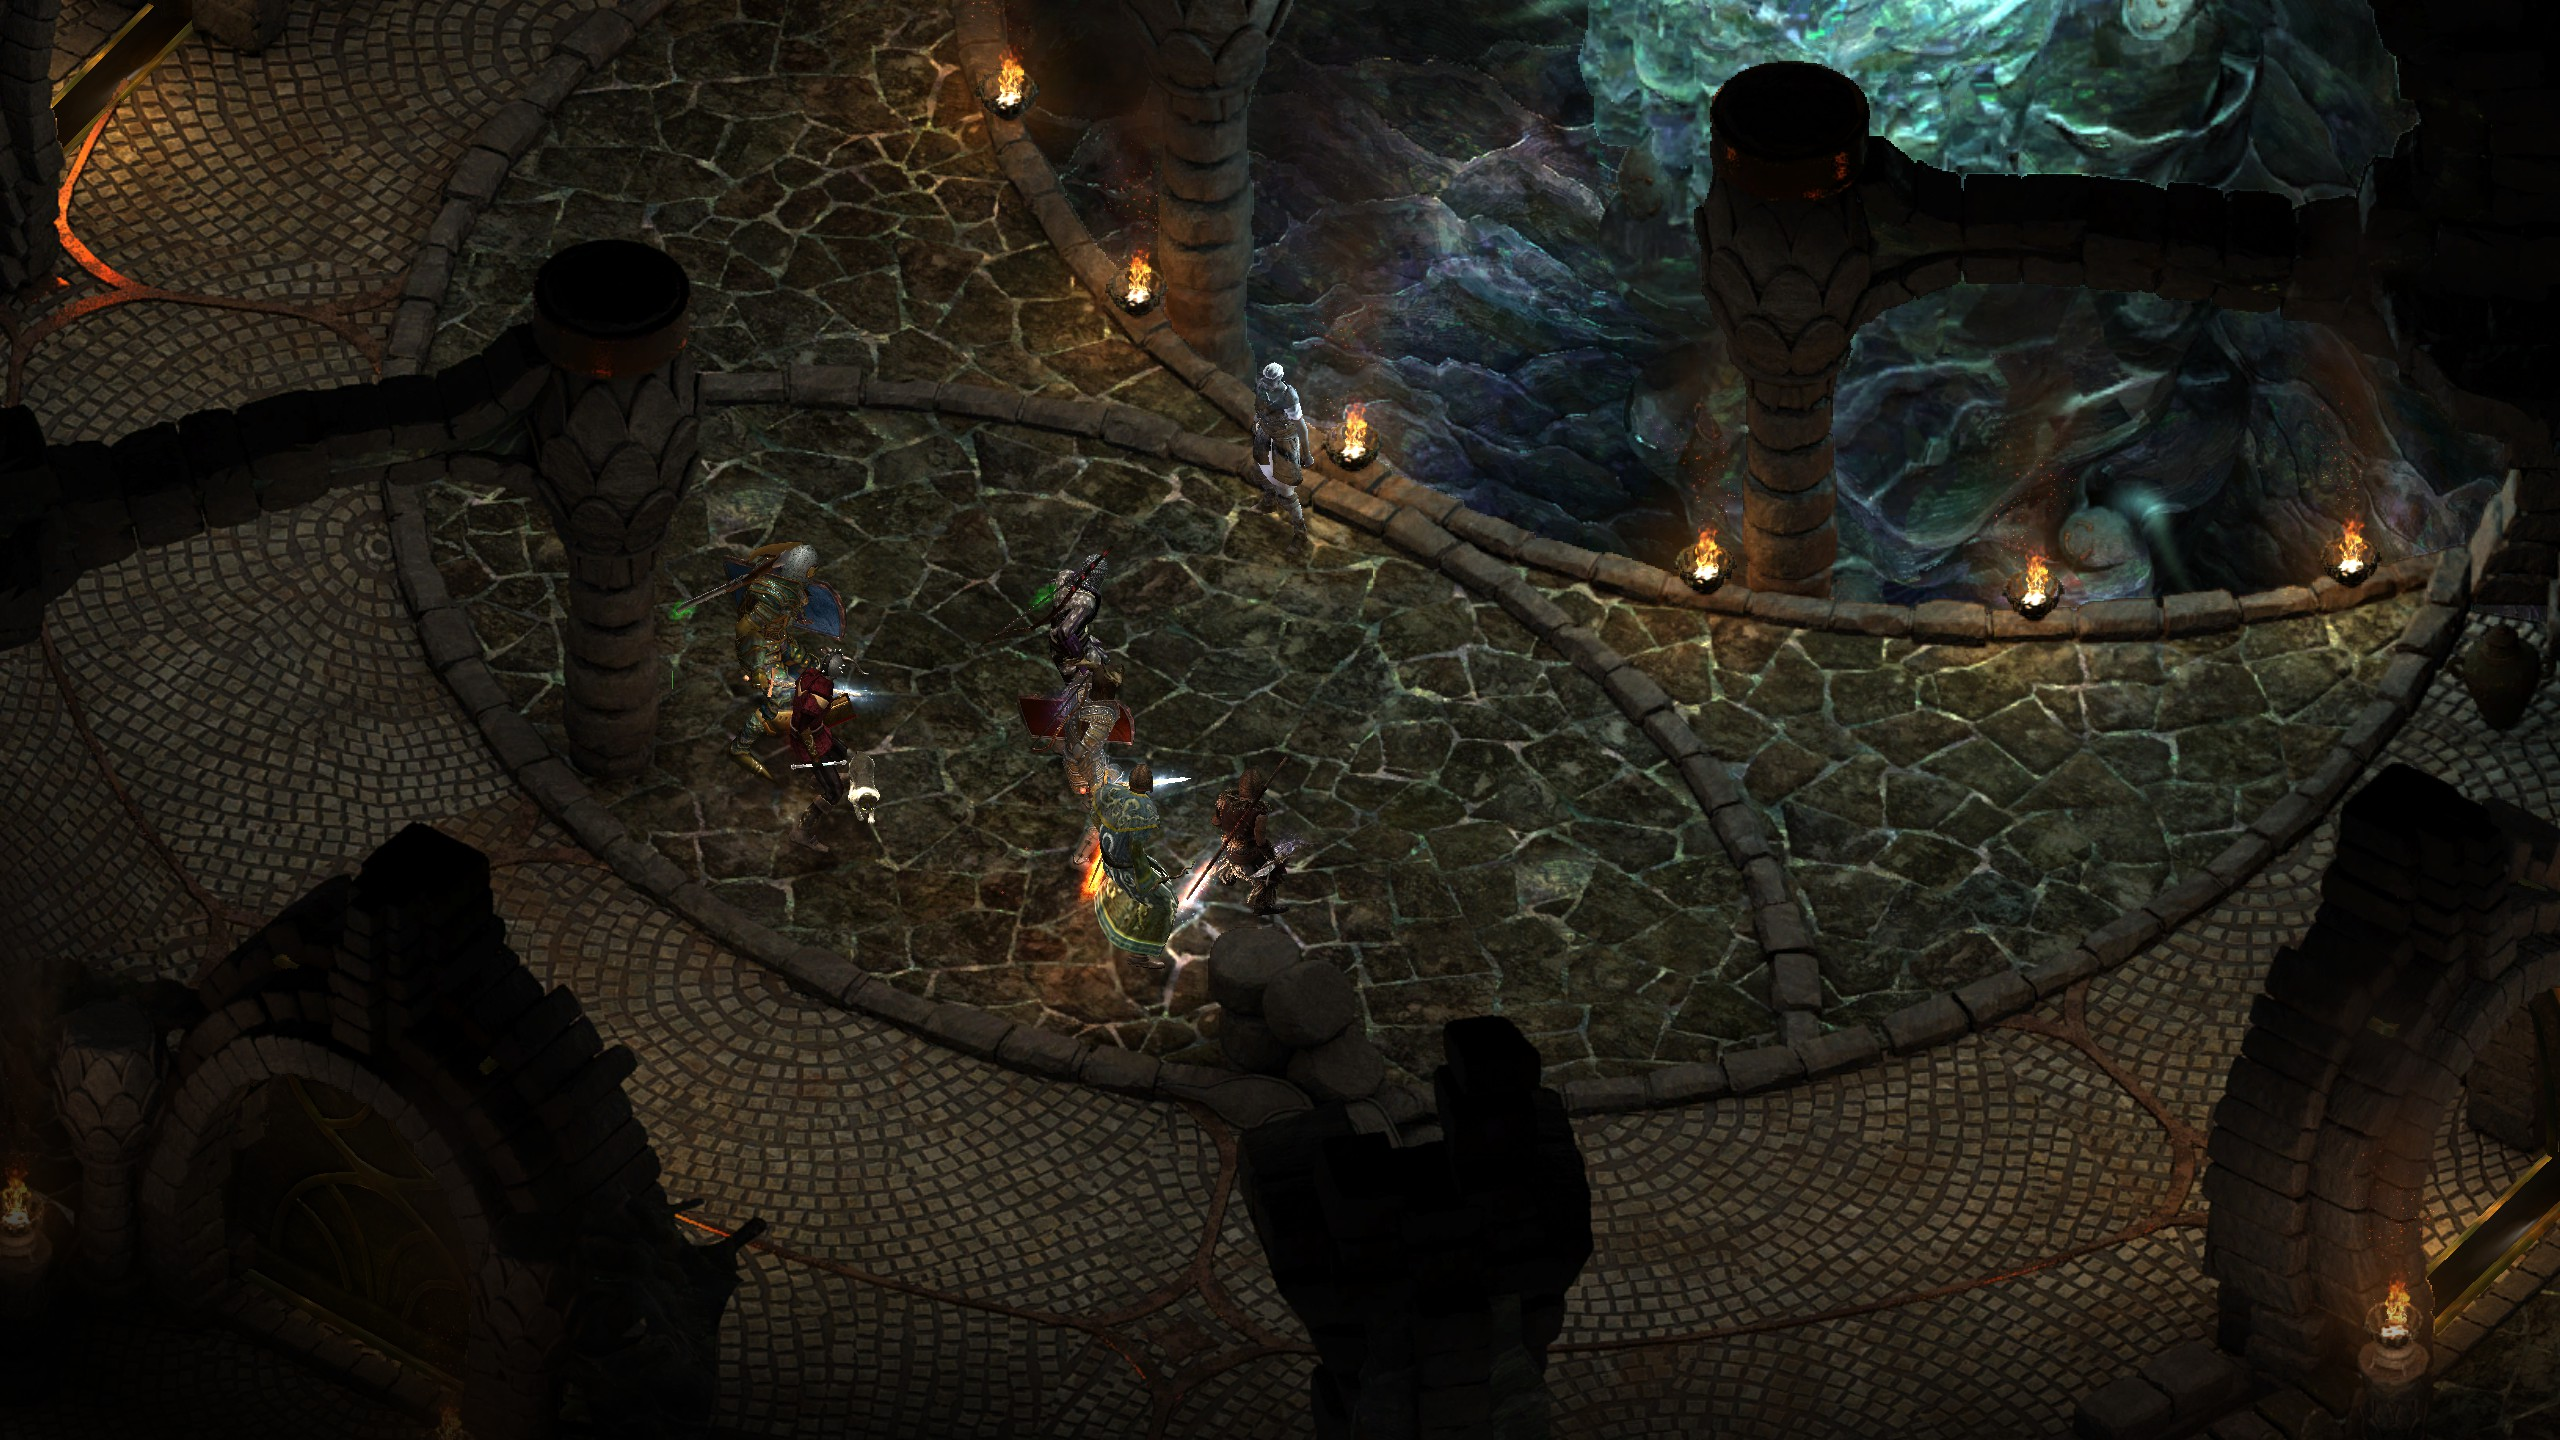
\includegraphics[scale=0.33]{files/blog/2019_03_17_pillars_of_eternity_path_of_the_damned_act_iv/2019_03_17_breith_eaman2.jpg}
\end{figure}

\subsubsection{Sun in Shadow}

The last area before Thaos was covered by an unnatural darkness, but the souls helped light the way forward.

\begin{figure}
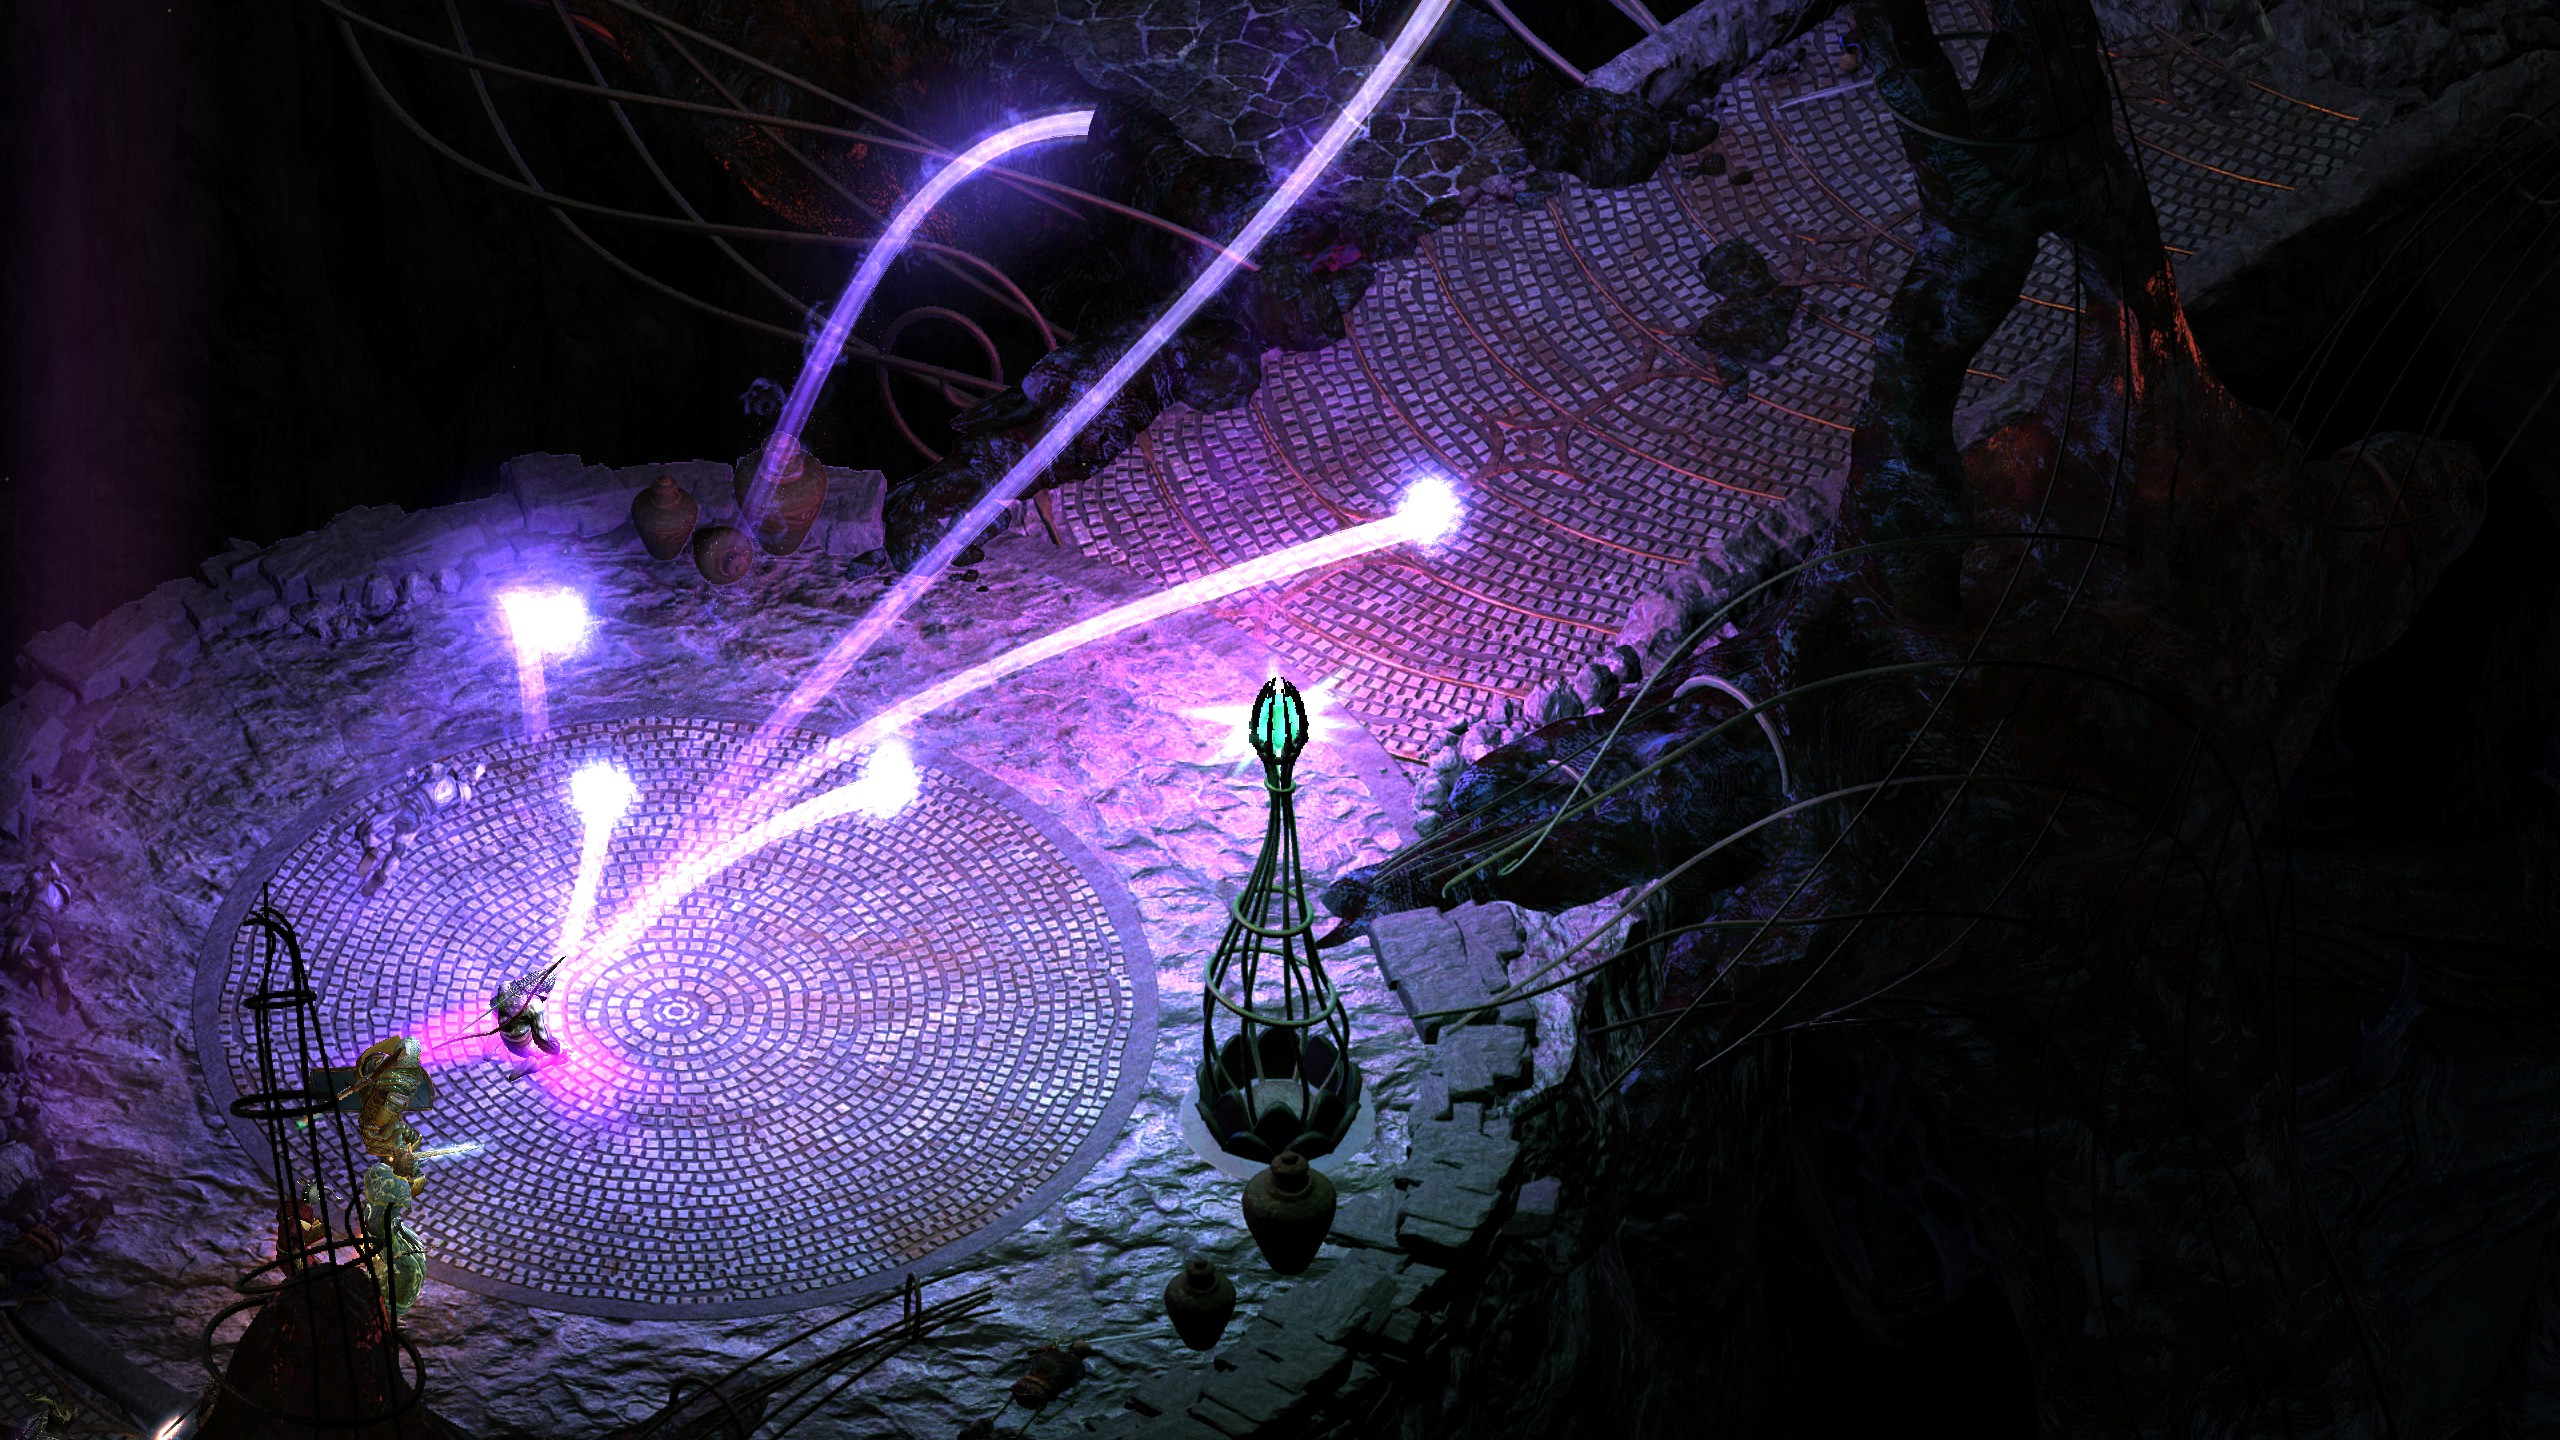
\includegraphics[scale=0.33]{files/blog/2019_03_17_pillars_of_eternity_path_of_the_damned_act_iv/2019_03_17_sun_in_shadow1.jpg}
\end{figure}

The area's shades were, of course, no problem to clear.

\begin{figure}
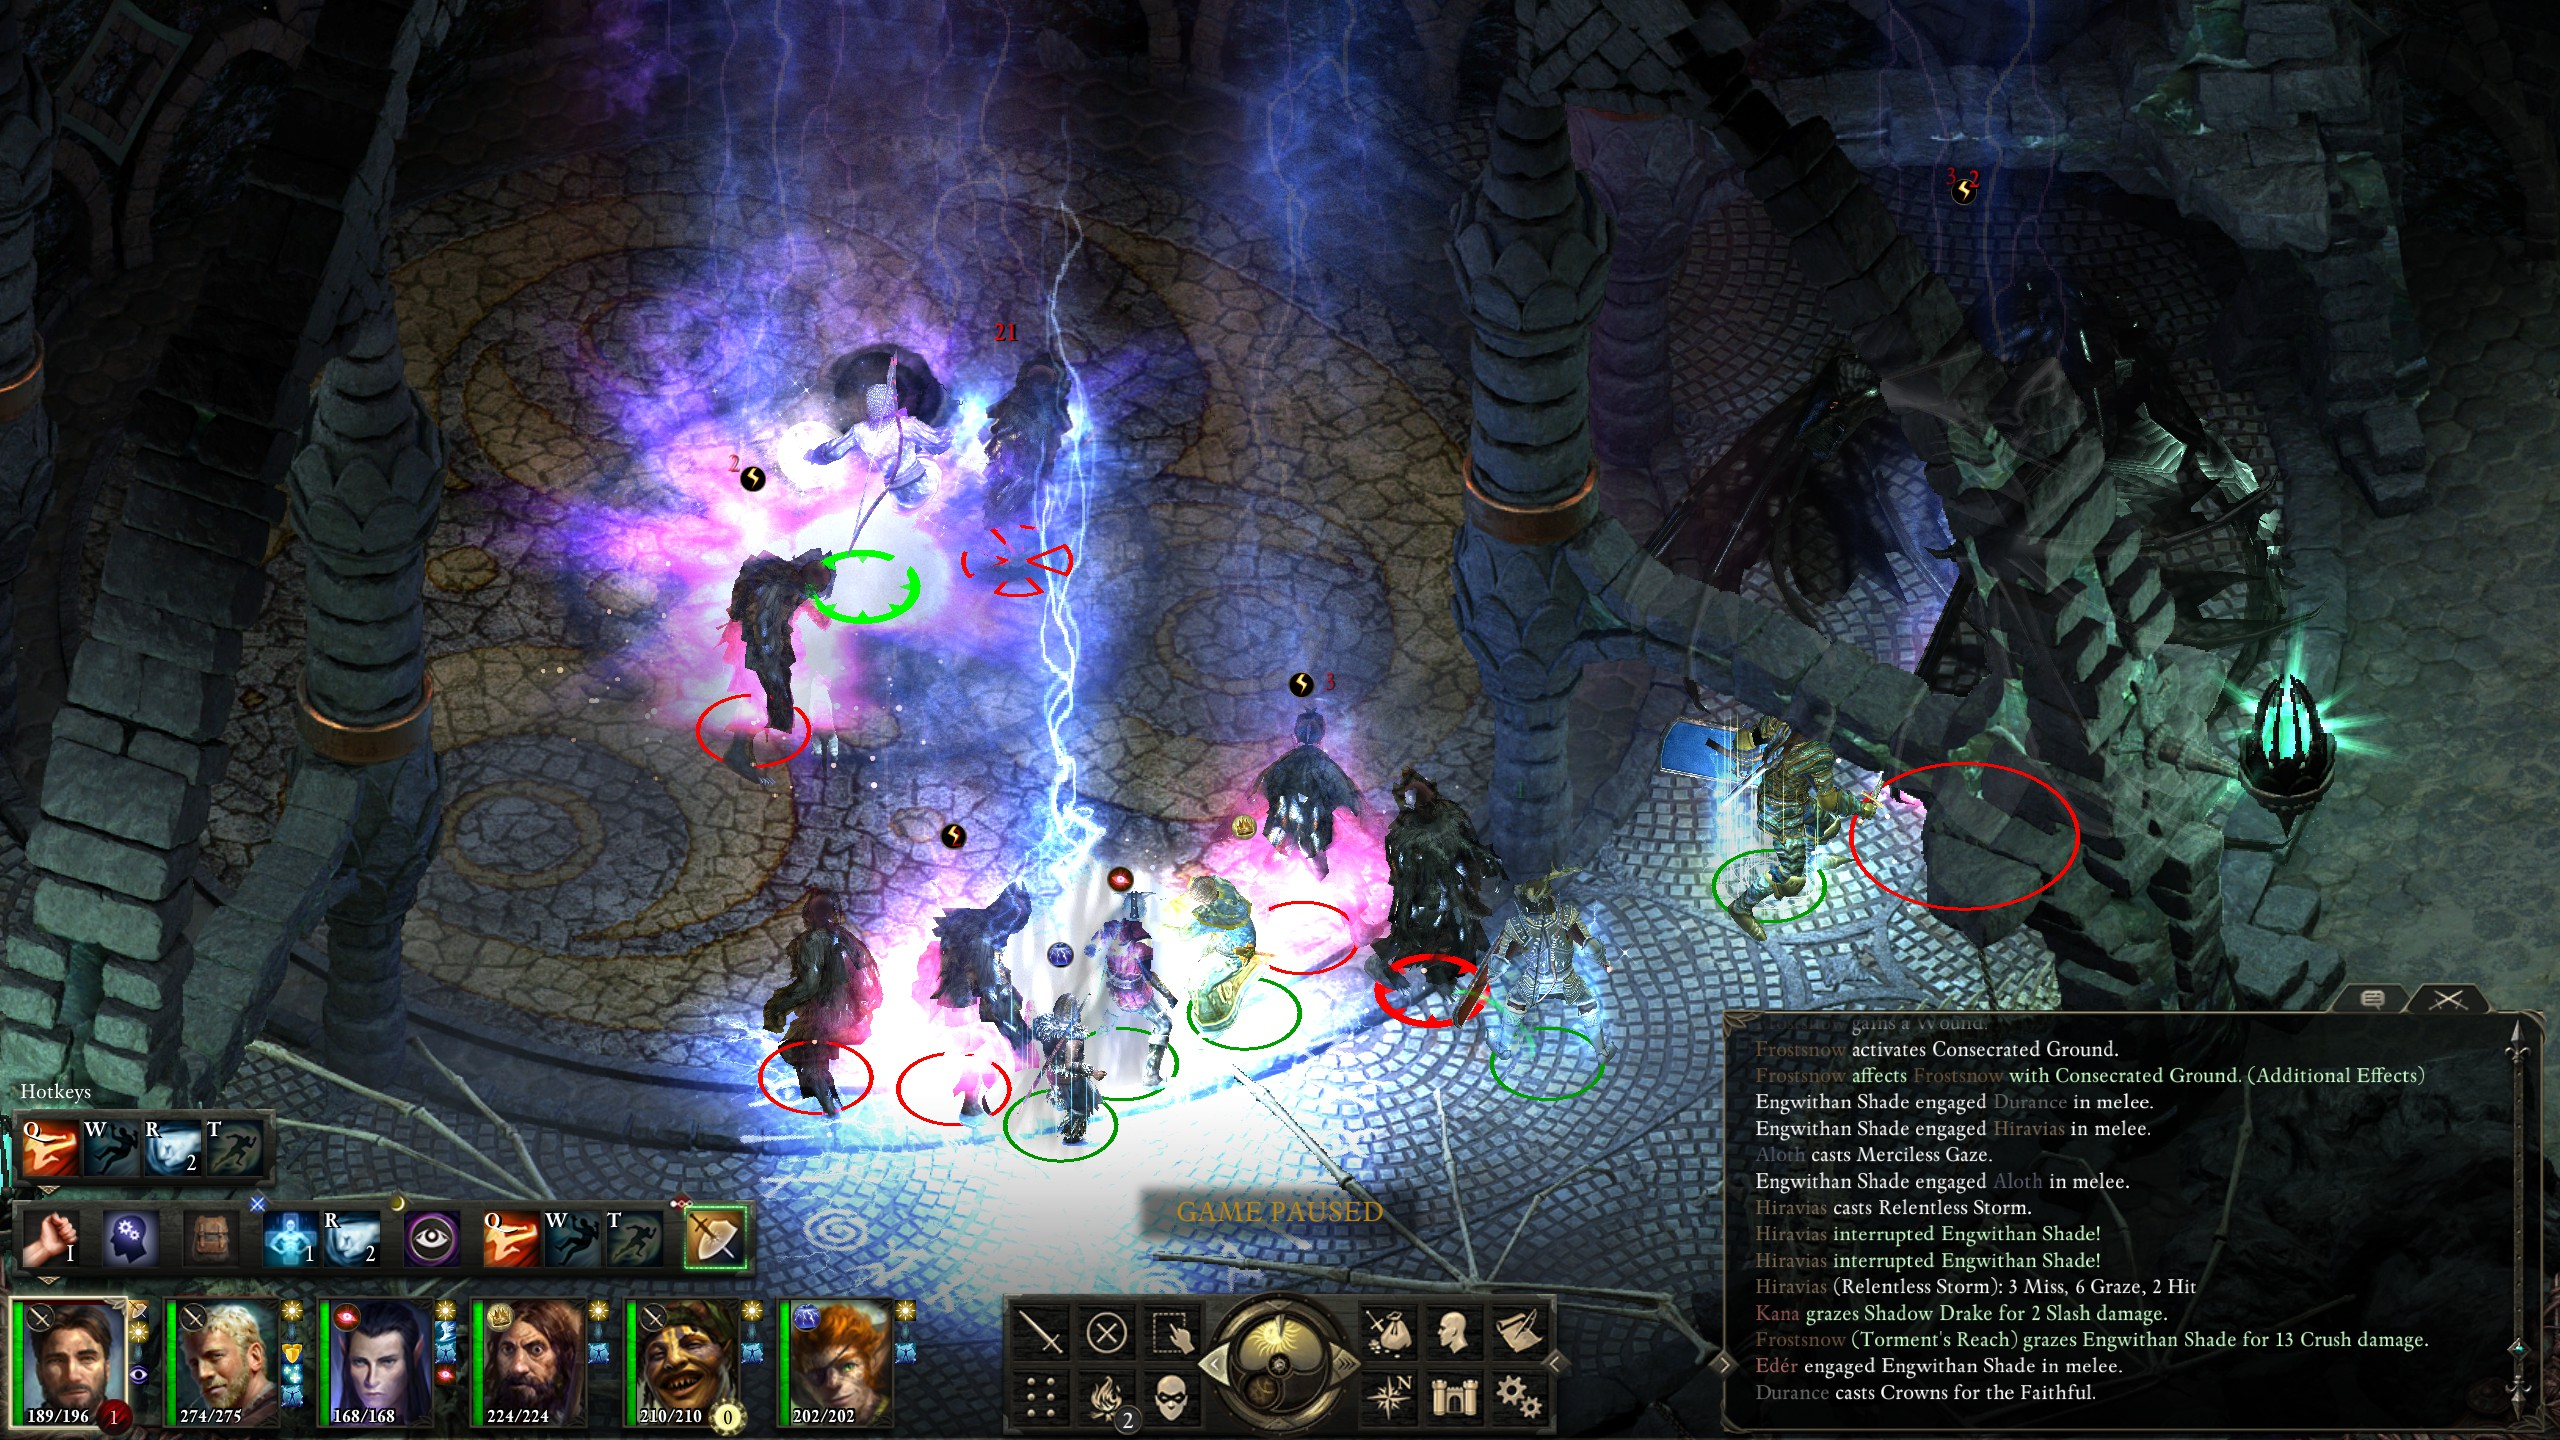
\includegraphics[scale=0.33]{files/blog/2019_03_17_pillars_of_eternity_path_of_the_damned_act_iv/2019_03_17_sun_in_shadow2.jpg}
\end{figure}

The shades thus gone, only Thaos was left.

\subsubsection{Thaos}

I wasn't really worried about Thaos.  Not after killing the Master Below.  Thaos may be though, but he's not that tough.

\begin{figure}
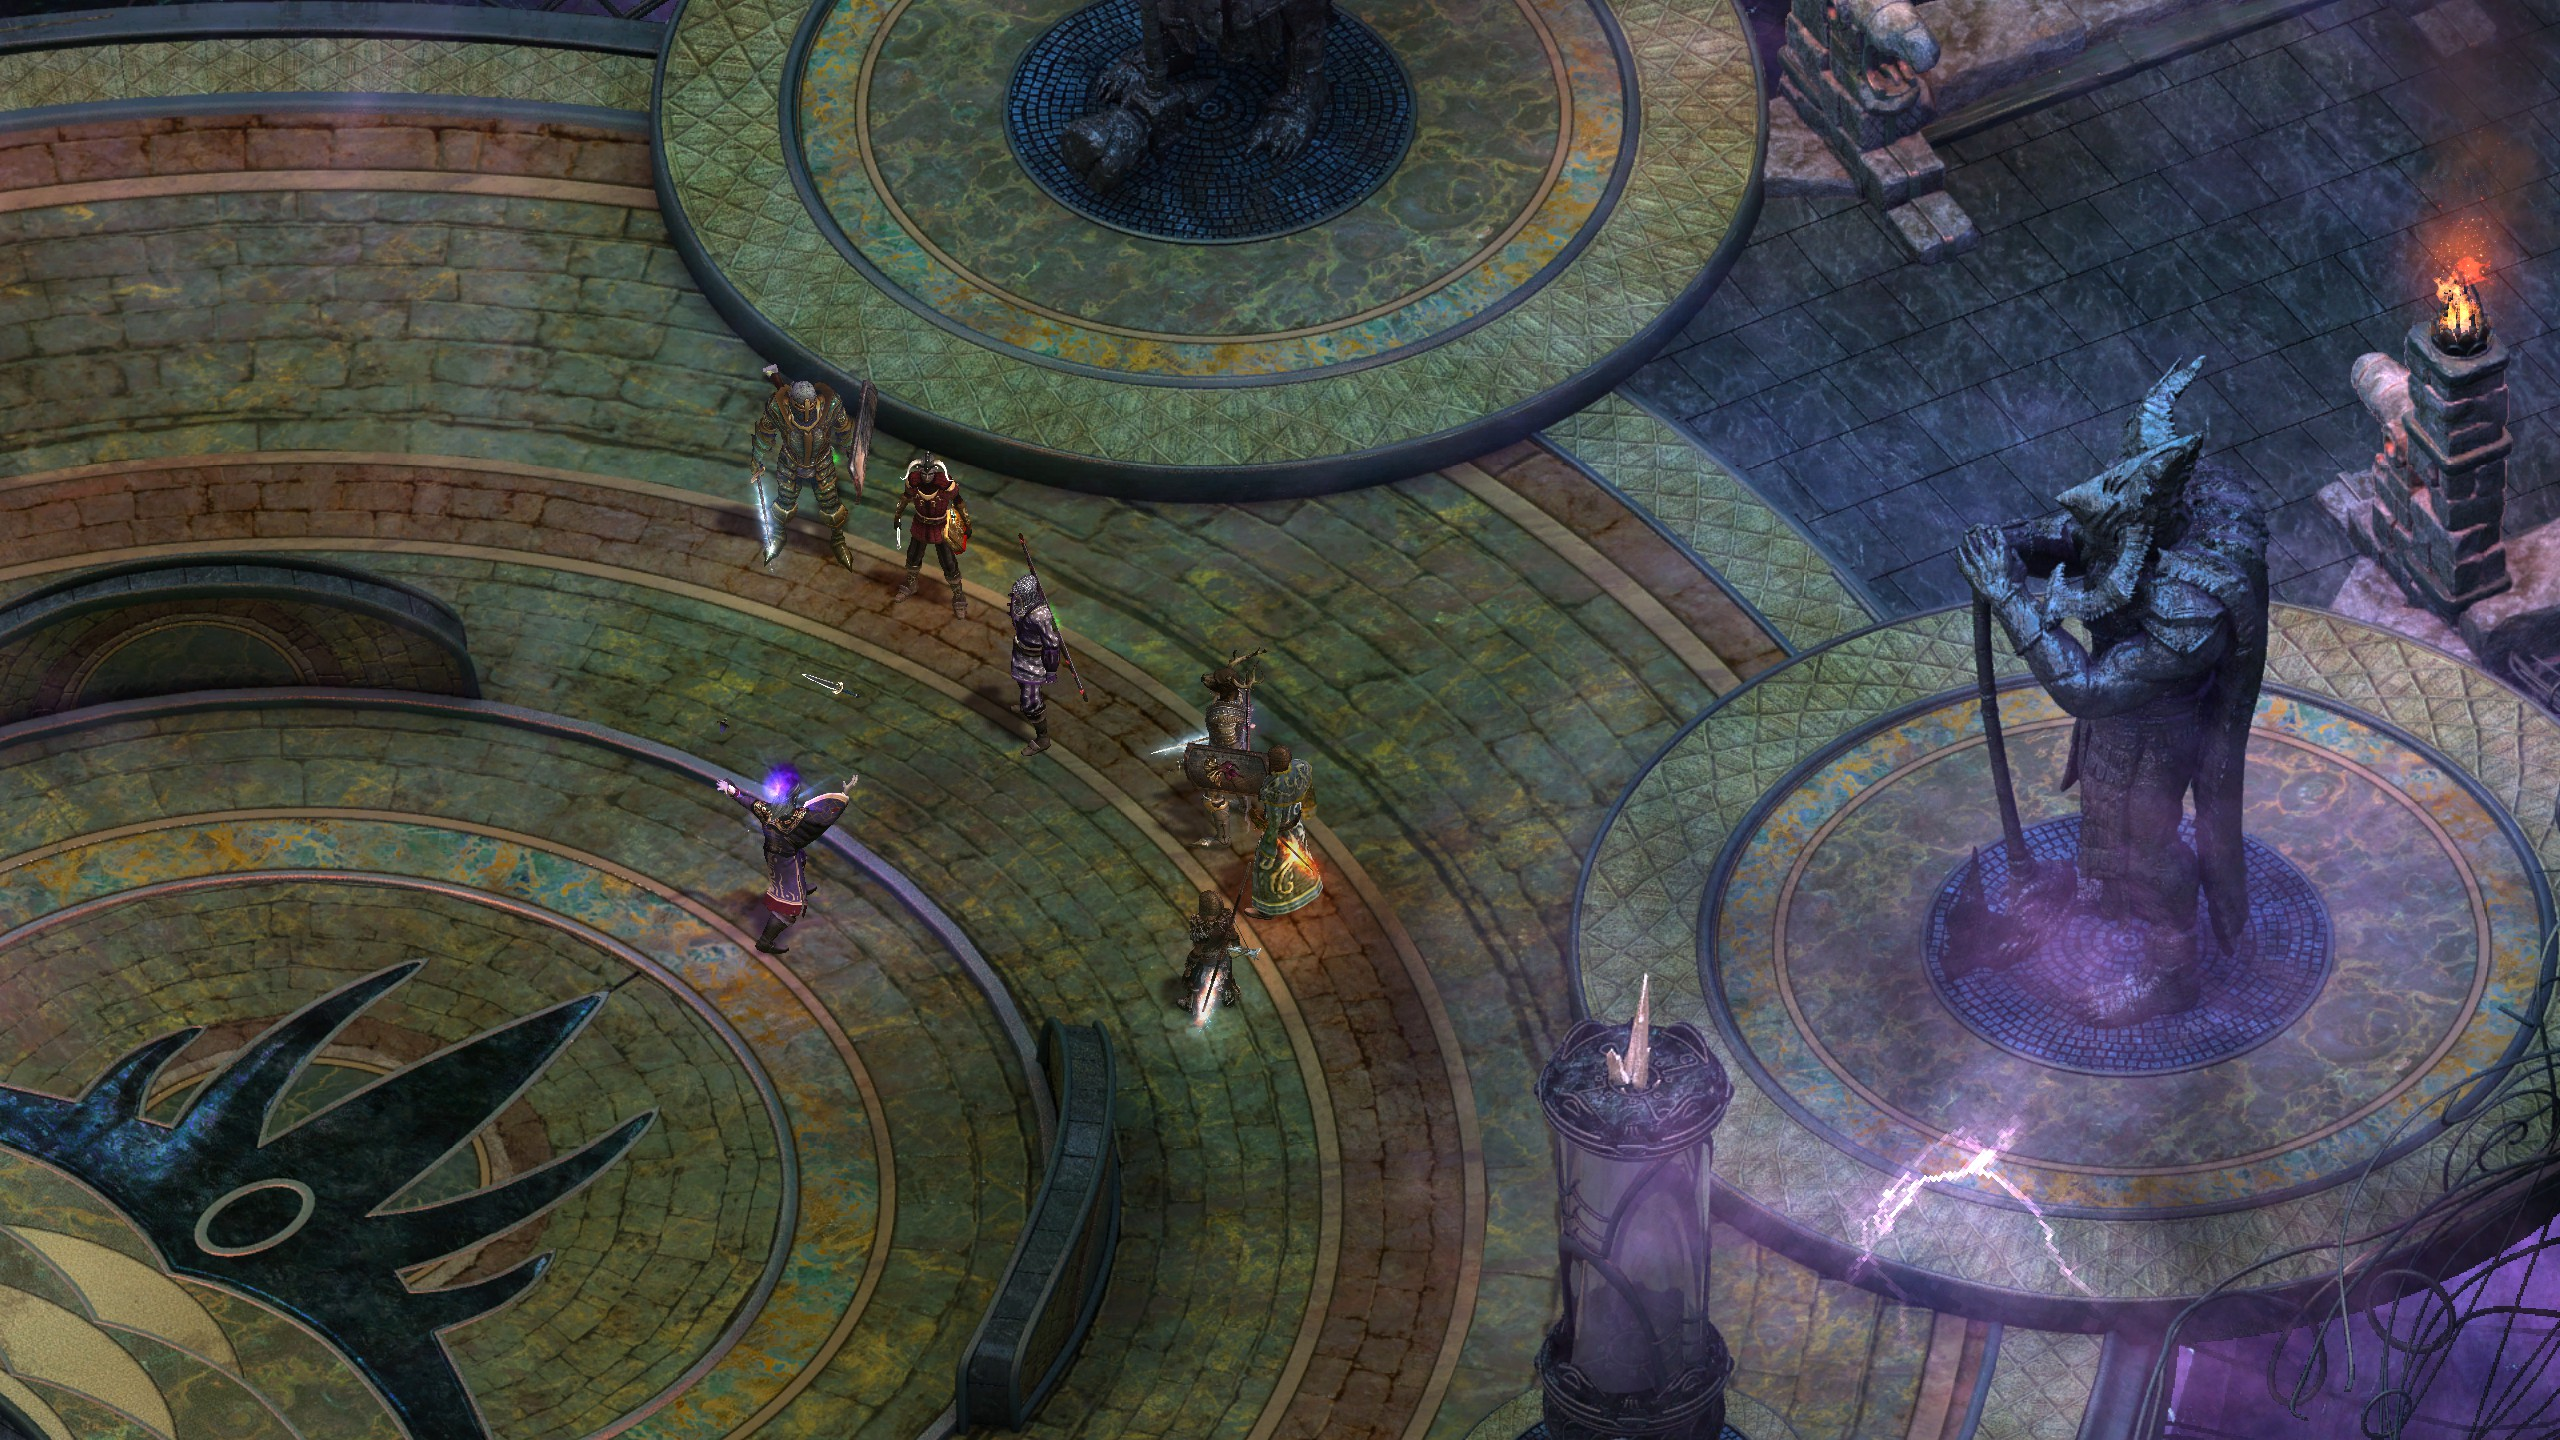
\includegraphics[scale=0.33]{files/blog/2019_03_17_pillars_of_eternity_path_of_the_damned_act_iv/2019_03_17_thaos0.jpg}
\end{figure}

That being said, Thaos wasn't going to simply hand me a victory; instead he decided to concentrate on Aloth, taking him down faster than I was prepared to heal him.  What a jerk!

\begin{figure}
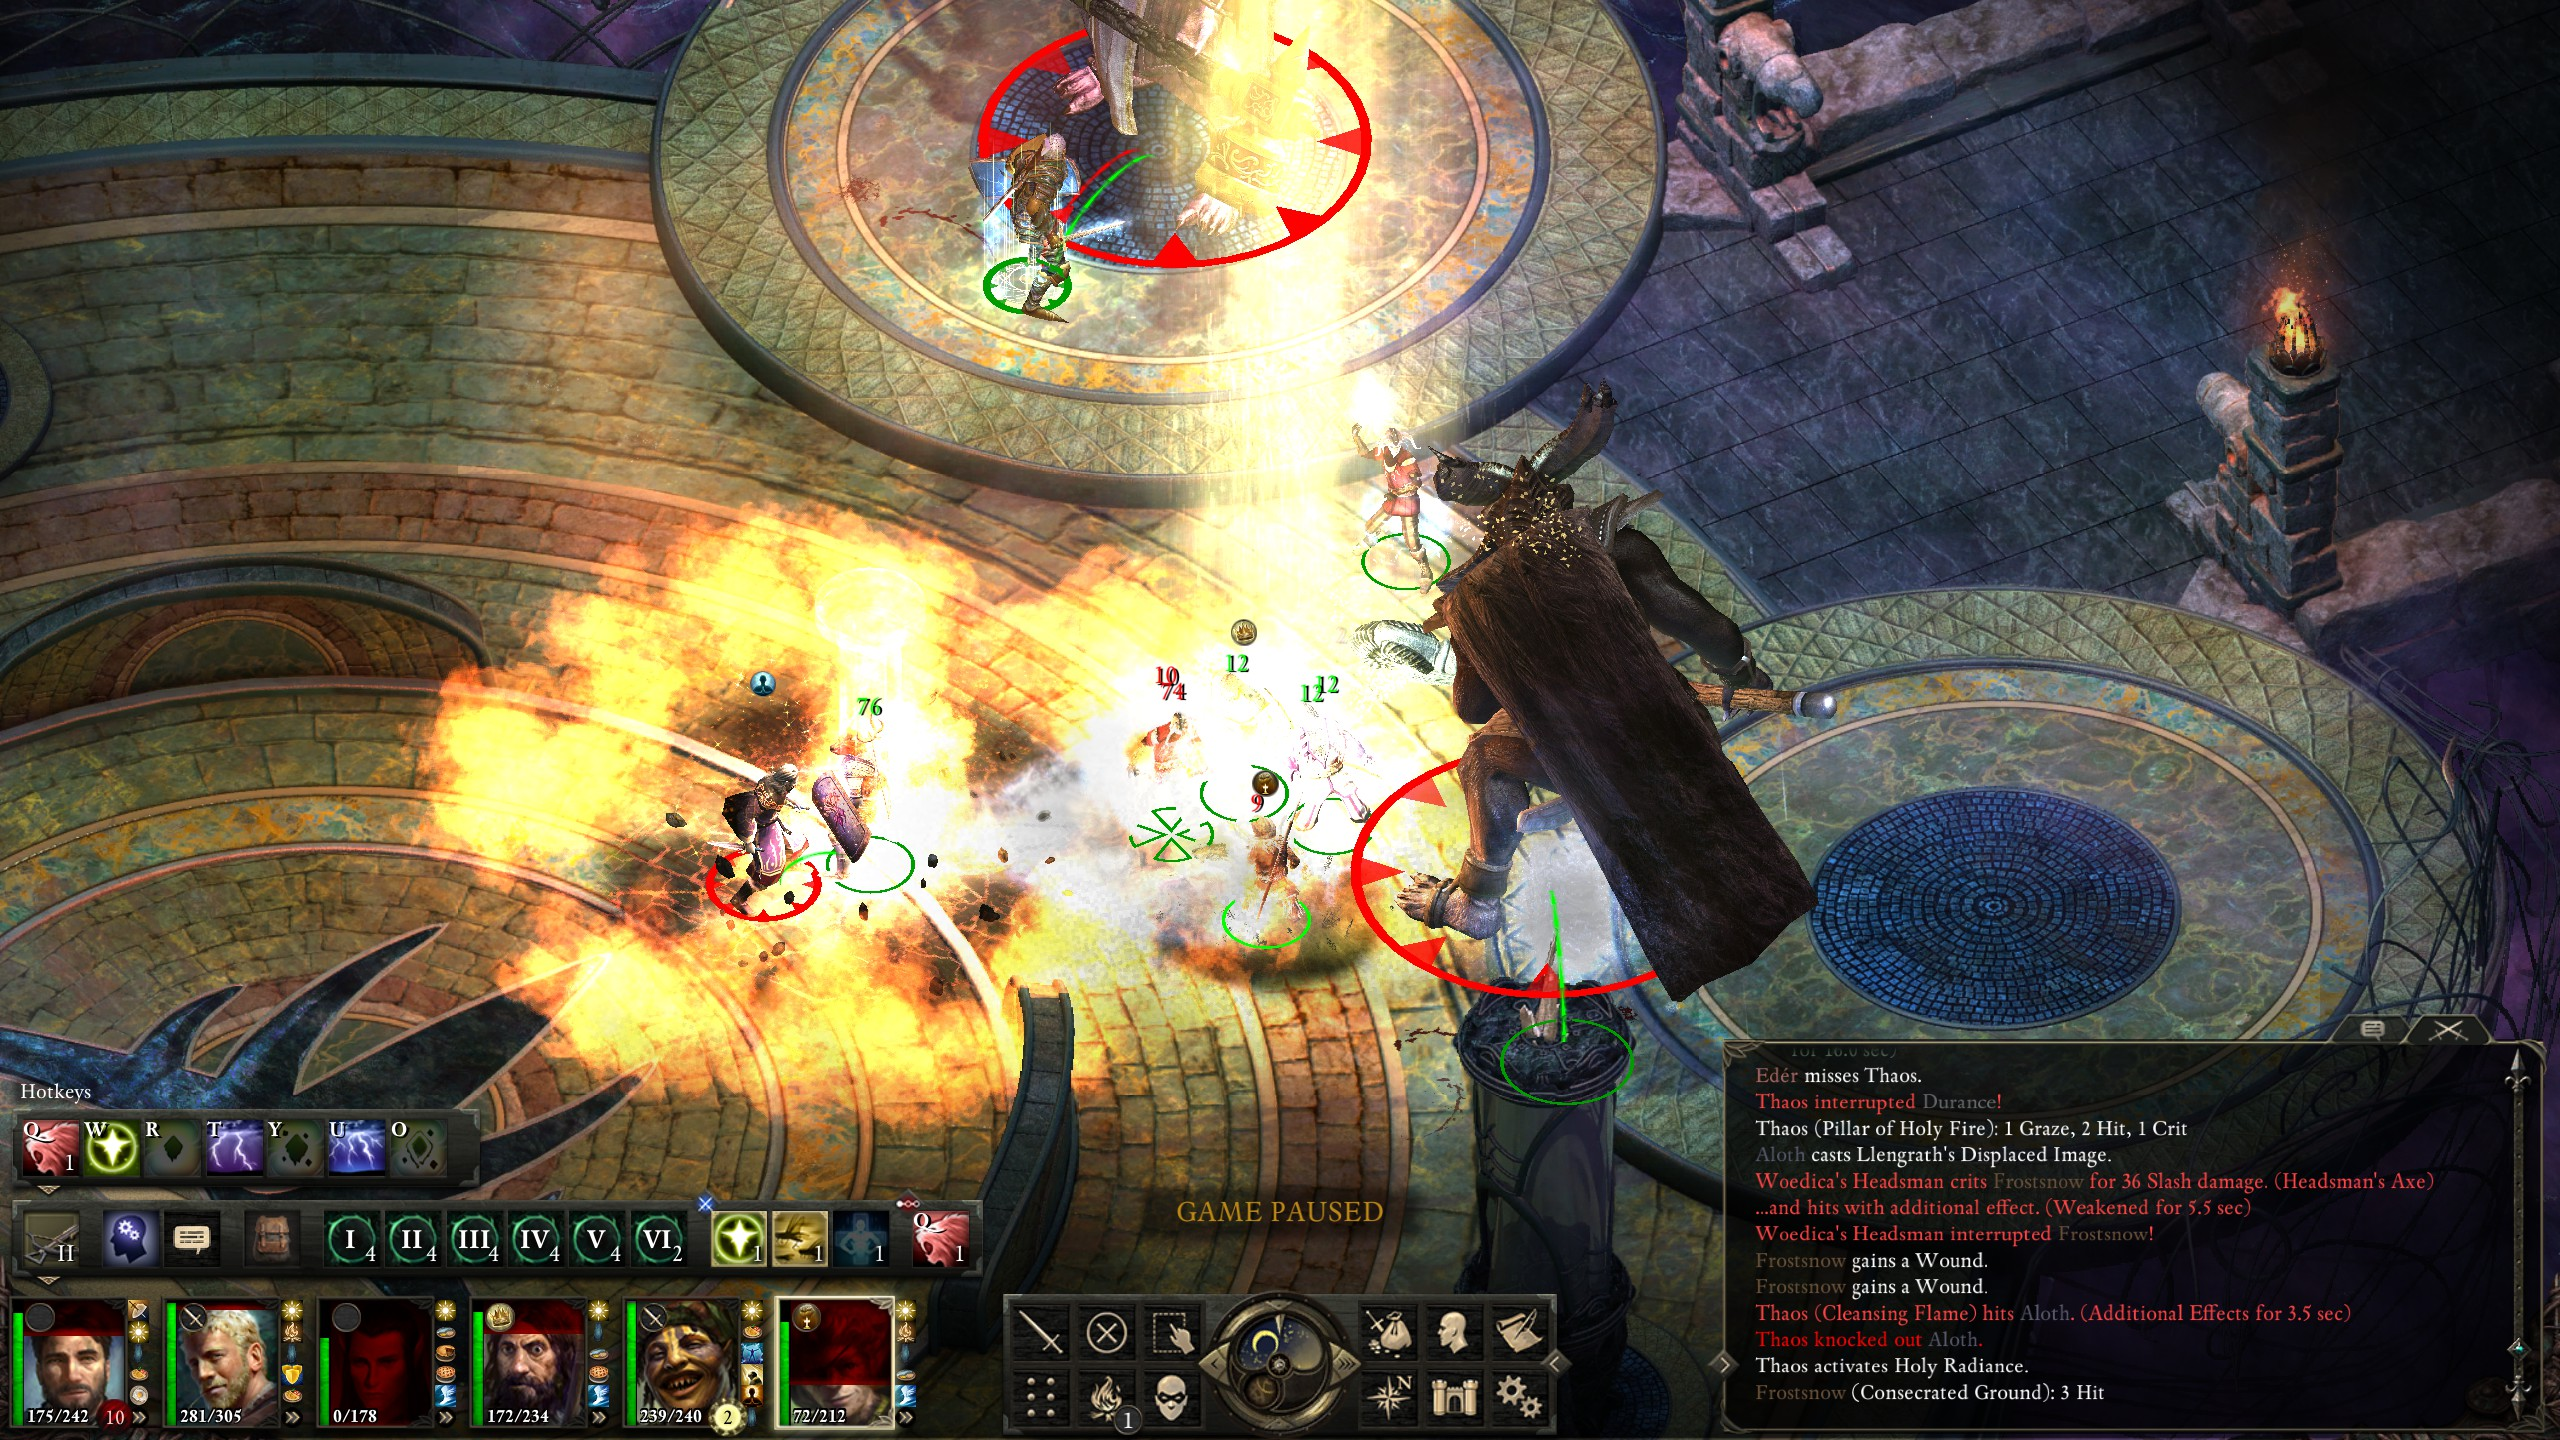
\includegraphics[scale=0.33]{files/blog/2019_03_17_pillars_of_eternity_path_of_the_damned_act_iv/2019_03_17_thaos1.jpg}
\end{figure}

Nonetheless, I quickly revived him (and had him cast a few defensive buffs on himself) and then proceeded to kill Woedica's Headsman.

\begin{figure}
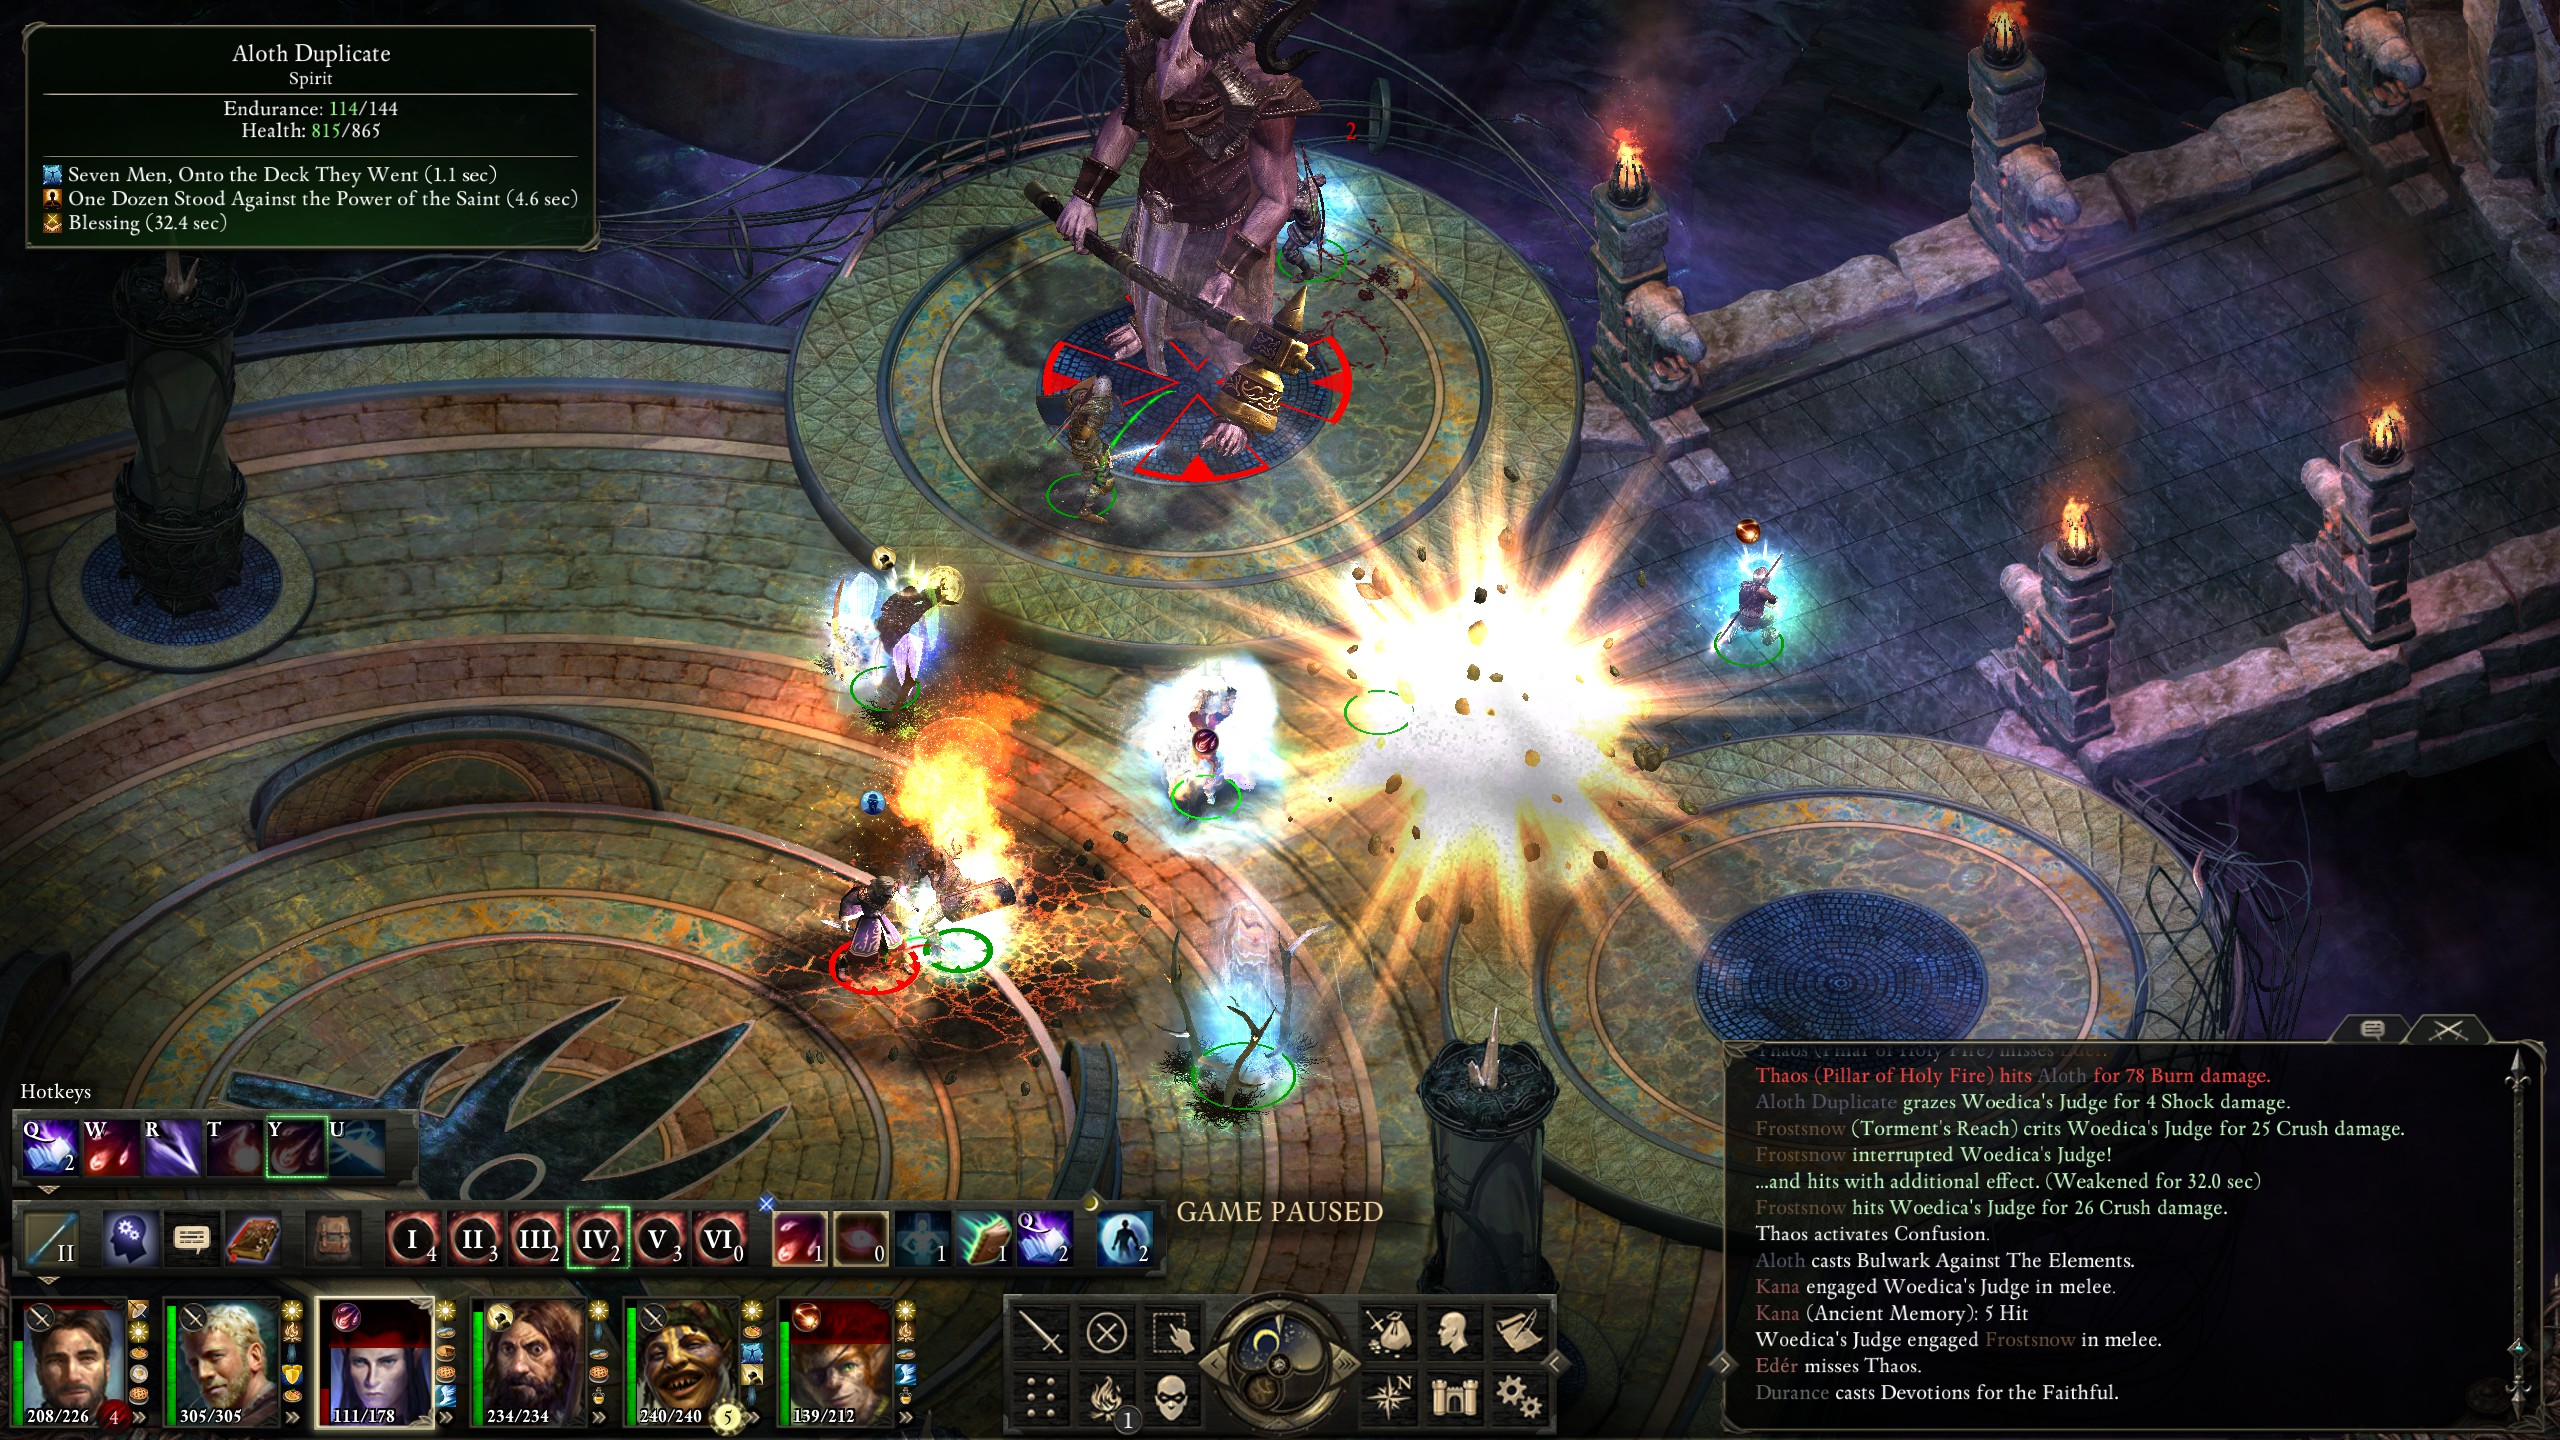
\includegraphics[scale=0.33]{files/blog/2019_03_17_pillars_of_eternity_path_of_the_damned_act_iv/2019_03_17_thaos2.jpg}
\end{figure}

Woedica's Judge then shared his friend's fate shortly thereafter.

\begin{figure}
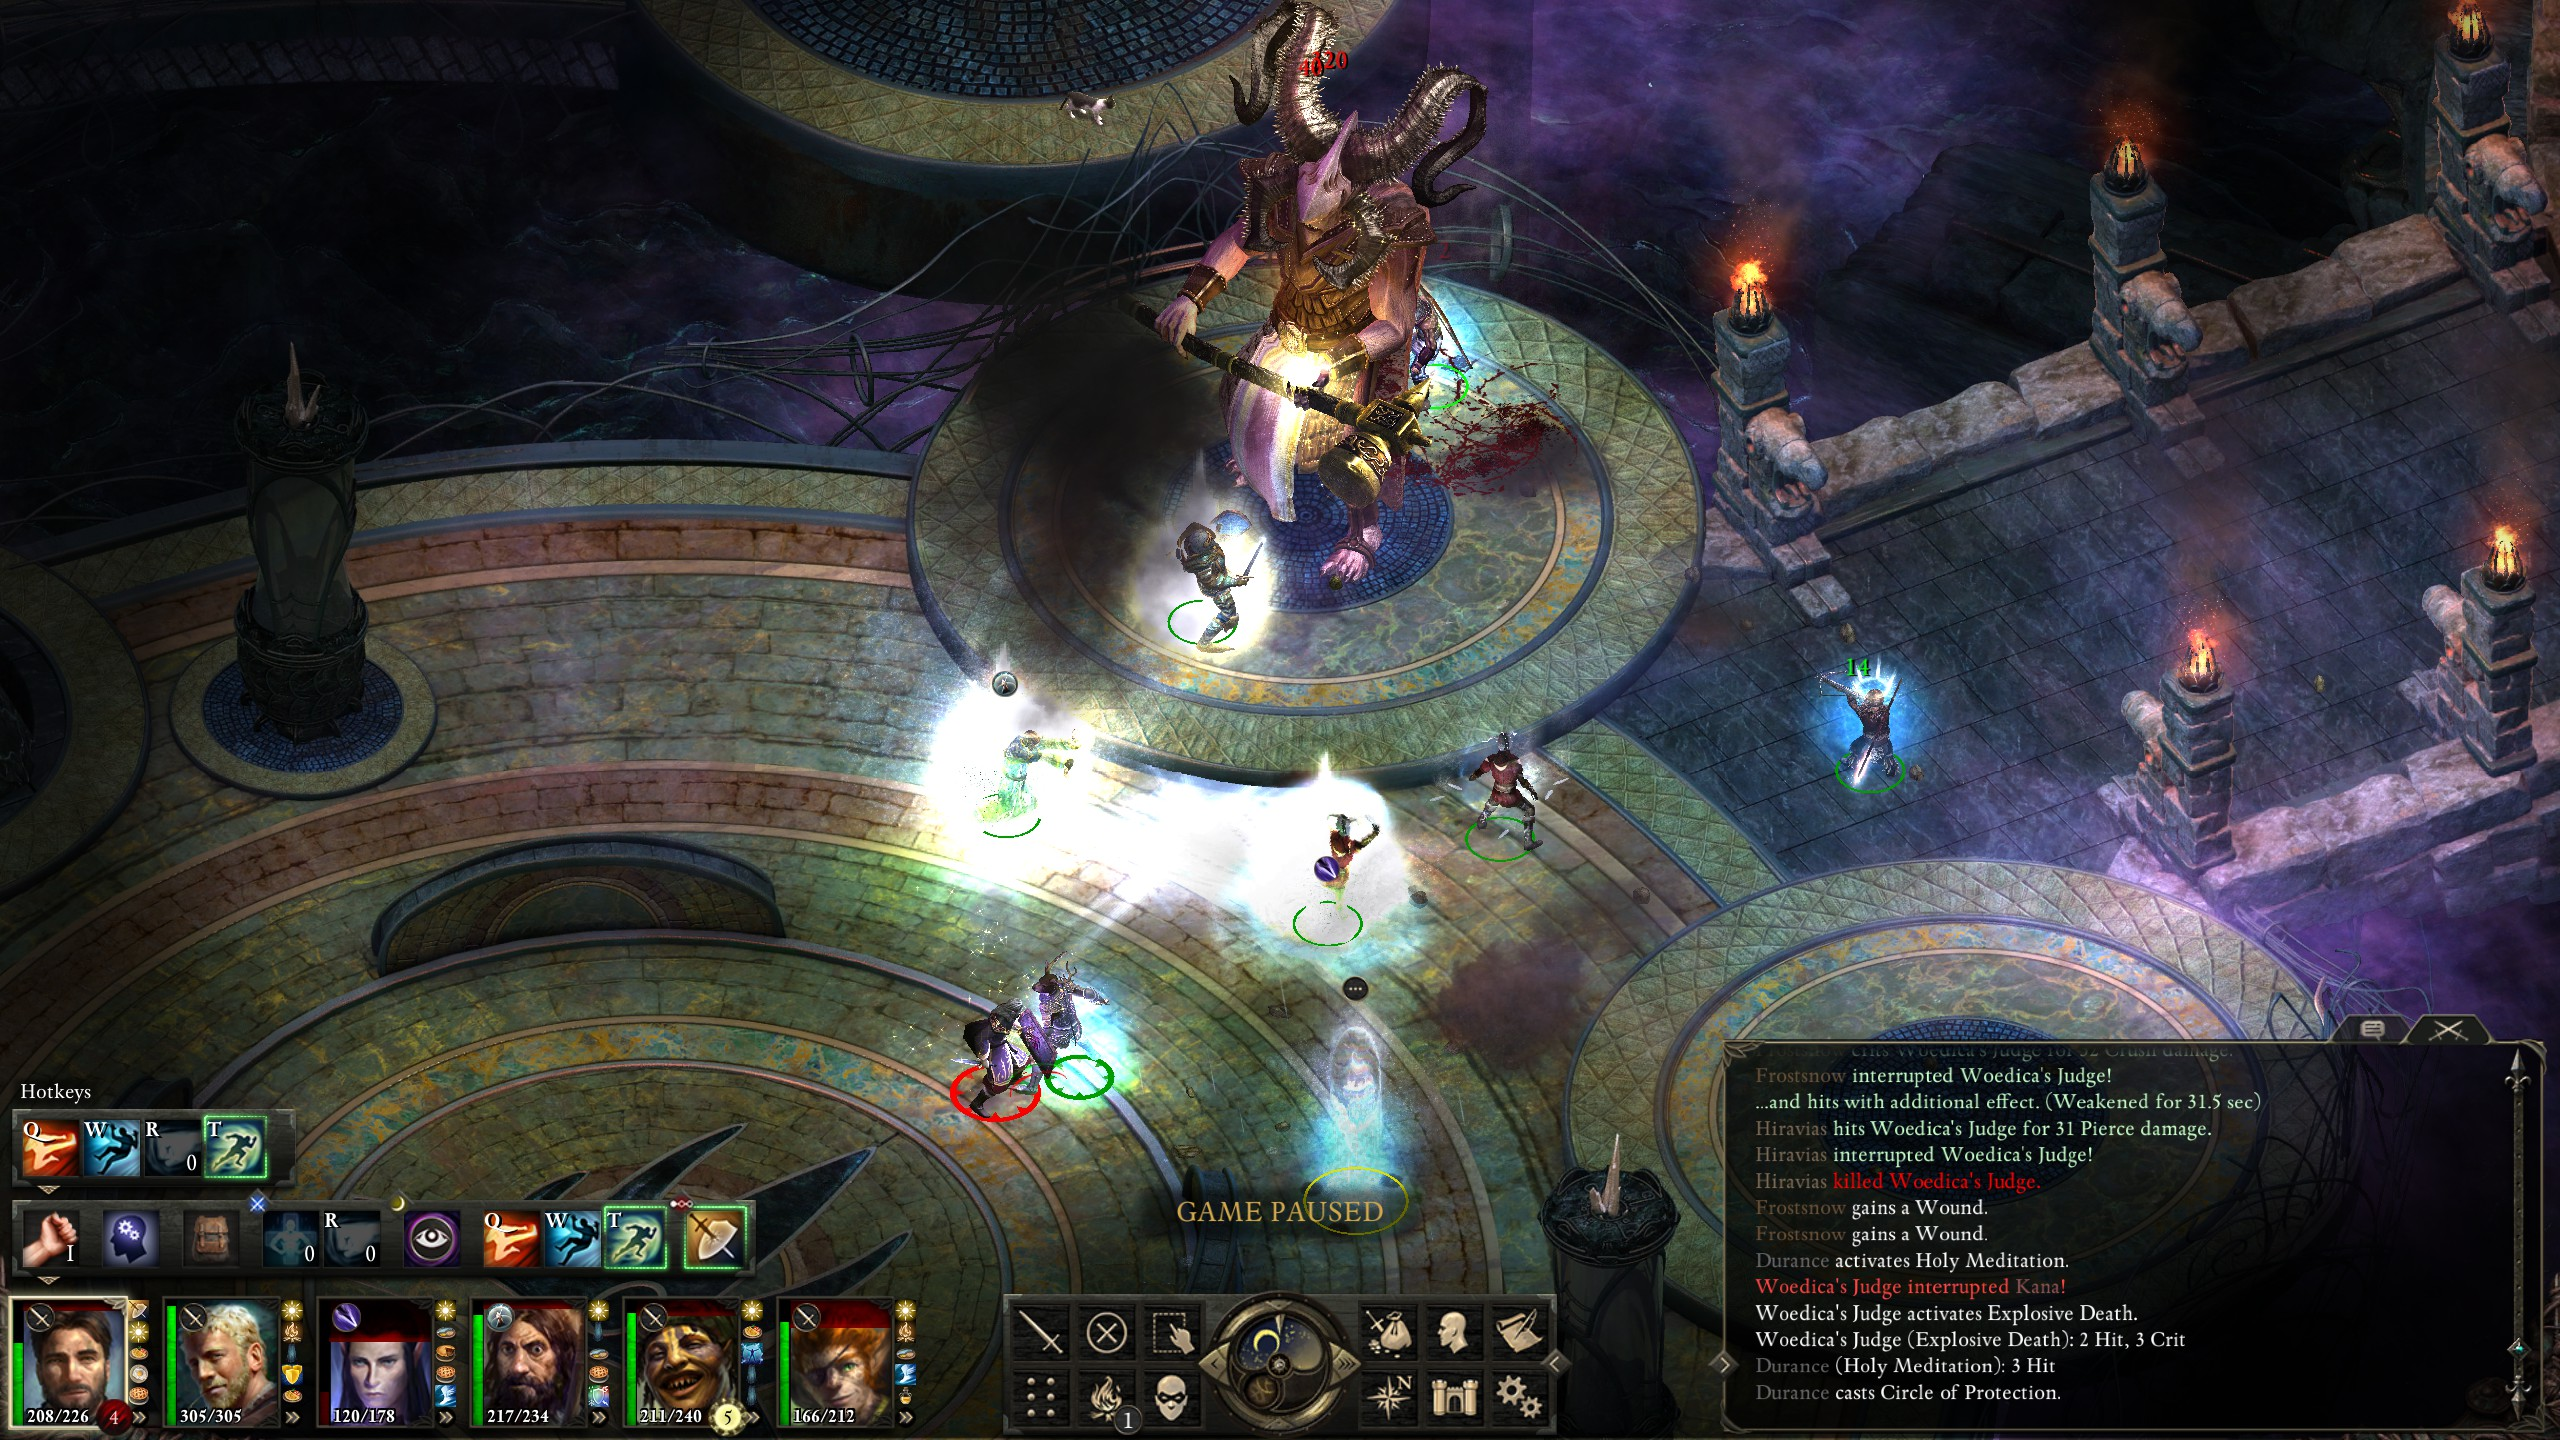
\includegraphics[scale=0.33]{files/blog/2019_03_17_pillars_of_eternity_path_of_the_damned_act_iv/2019_03_17_thaos3.jpg}
\end{figure}

I then quickly surrounded Thaos.  Thaos himself is tricky to kill in part because he's highly buffed, but he will also use an AoE dominate/charm spell when he gets low in order to take the damage off of him while he then heals back up; the damage, dominate, heal cycle can repeat while he wears the party down, so I had to put a stop to it.  The first thing was to cast Aloth's "Arkemyr's Wondrous Torment" to weaken Thaos' casting ability followed by "Arcane Dampener" to suppress his buffs; meanwhile, Durance cast "Crowns for the Faithful" on those surrounding Thaos for the extra +62 to Will saves.

\begin{figure}
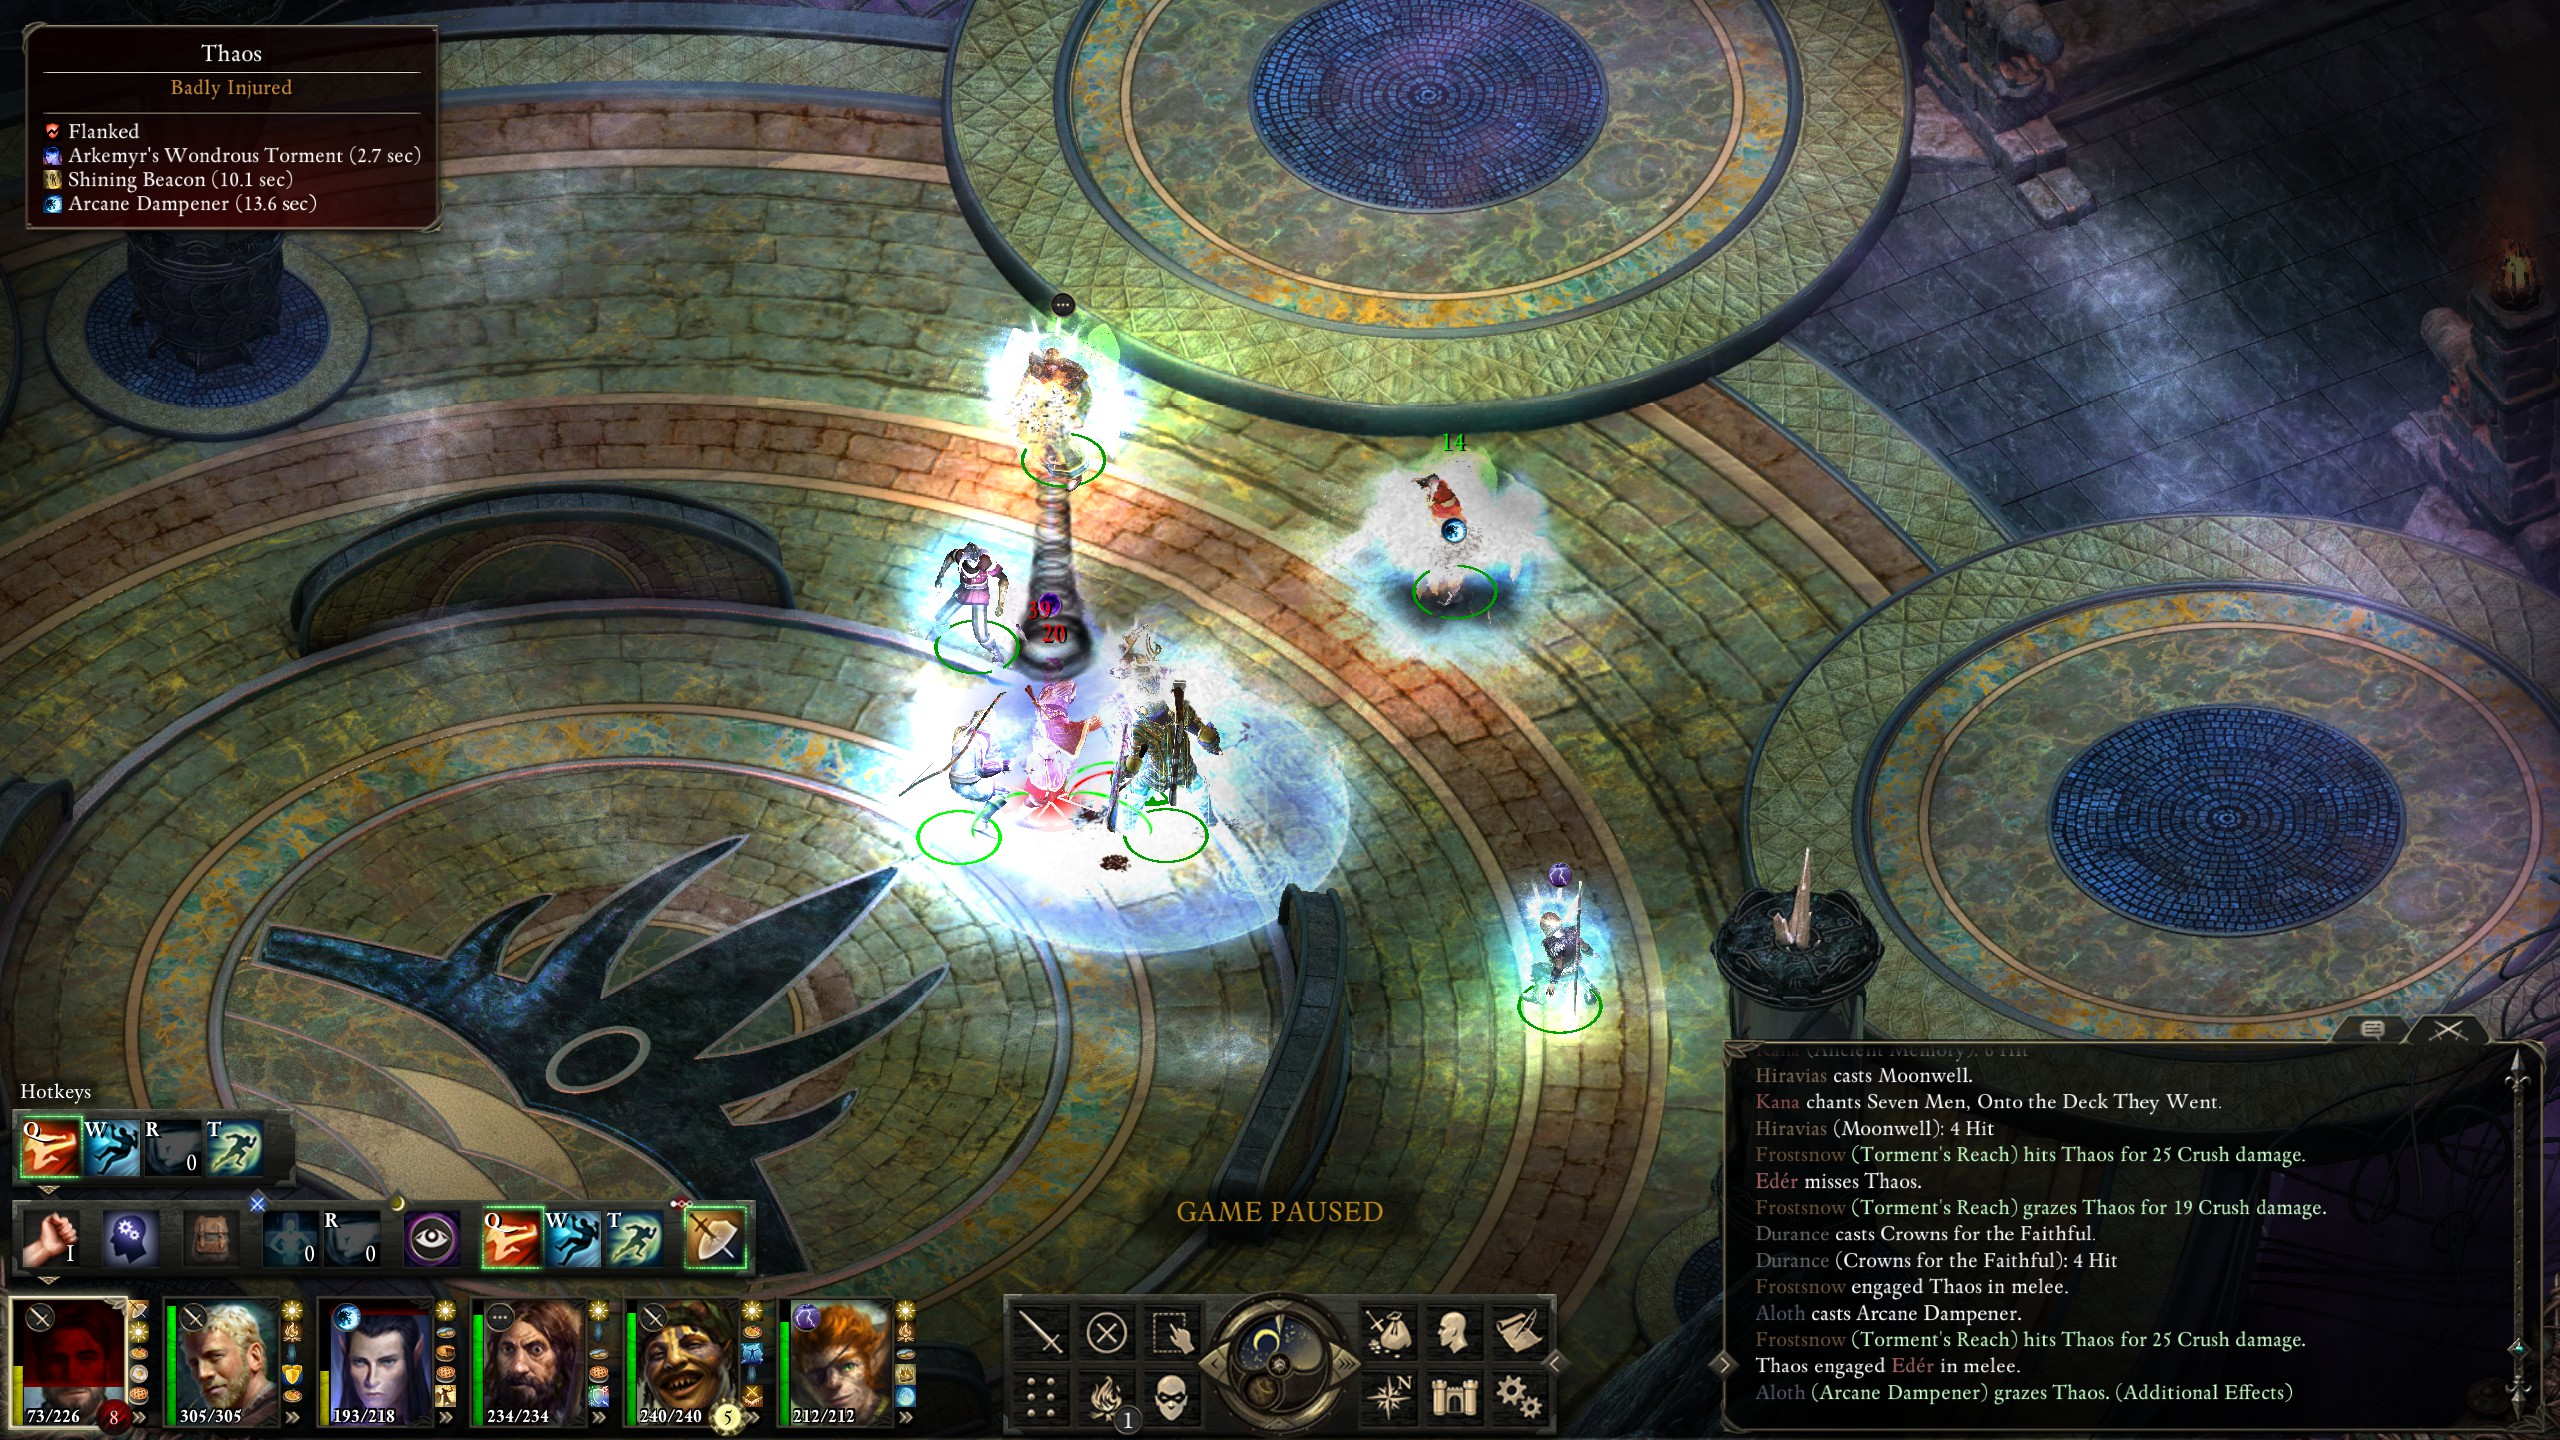
\includegraphics[scale=0.33]{files/blog/2019_03_17_pillars_of_eternity_path_of_the_damned_act_iv/2019_03_17_thaos4.jpg}
\end{figure}

Thus when Thaos finally cast his dominate spell, the only ones affected were my monk and an Aloth duplicate.

\begin{figure}
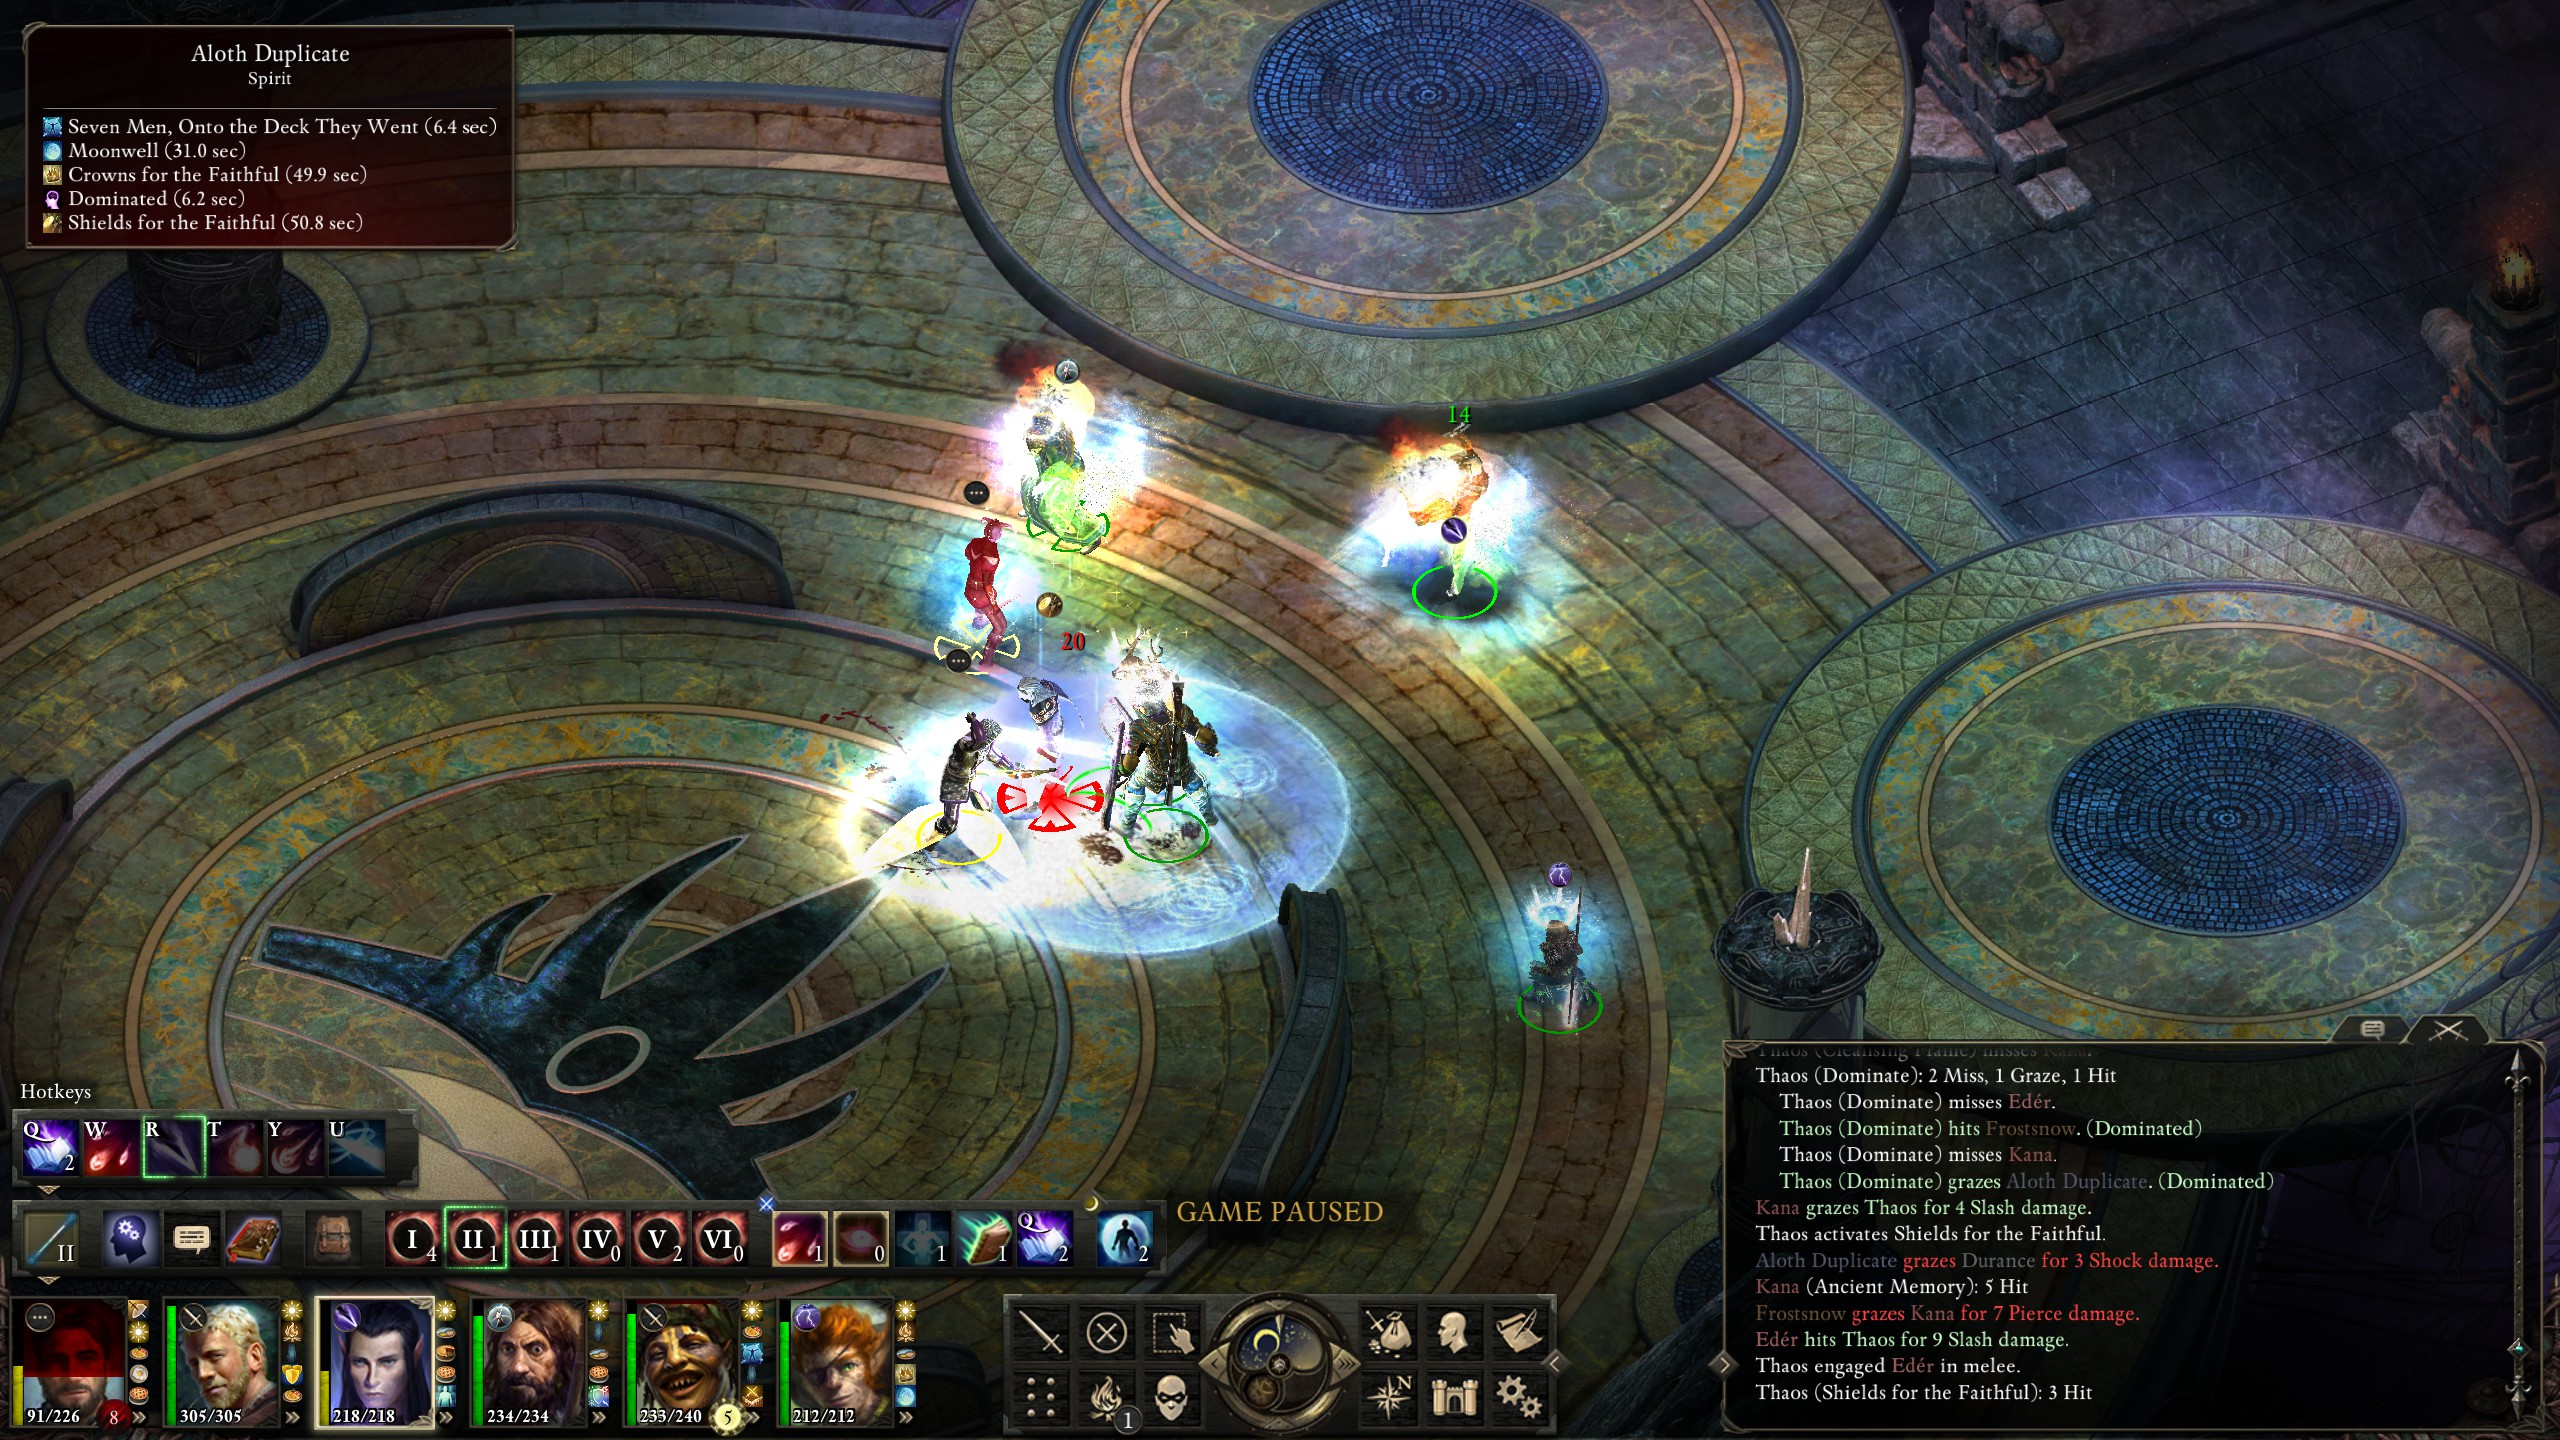
\includegraphics[scale=0.33]{files/blog/2019_03_17_pillars_of_eternity_path_of_the_damned_act_iv/2019_03_17_thaos5.jpg}
\end{figure}

Hiravas then got a fortunate "Returning Storm" proc on Thaos, stunning him, and he quickly died.

\begin{figure}
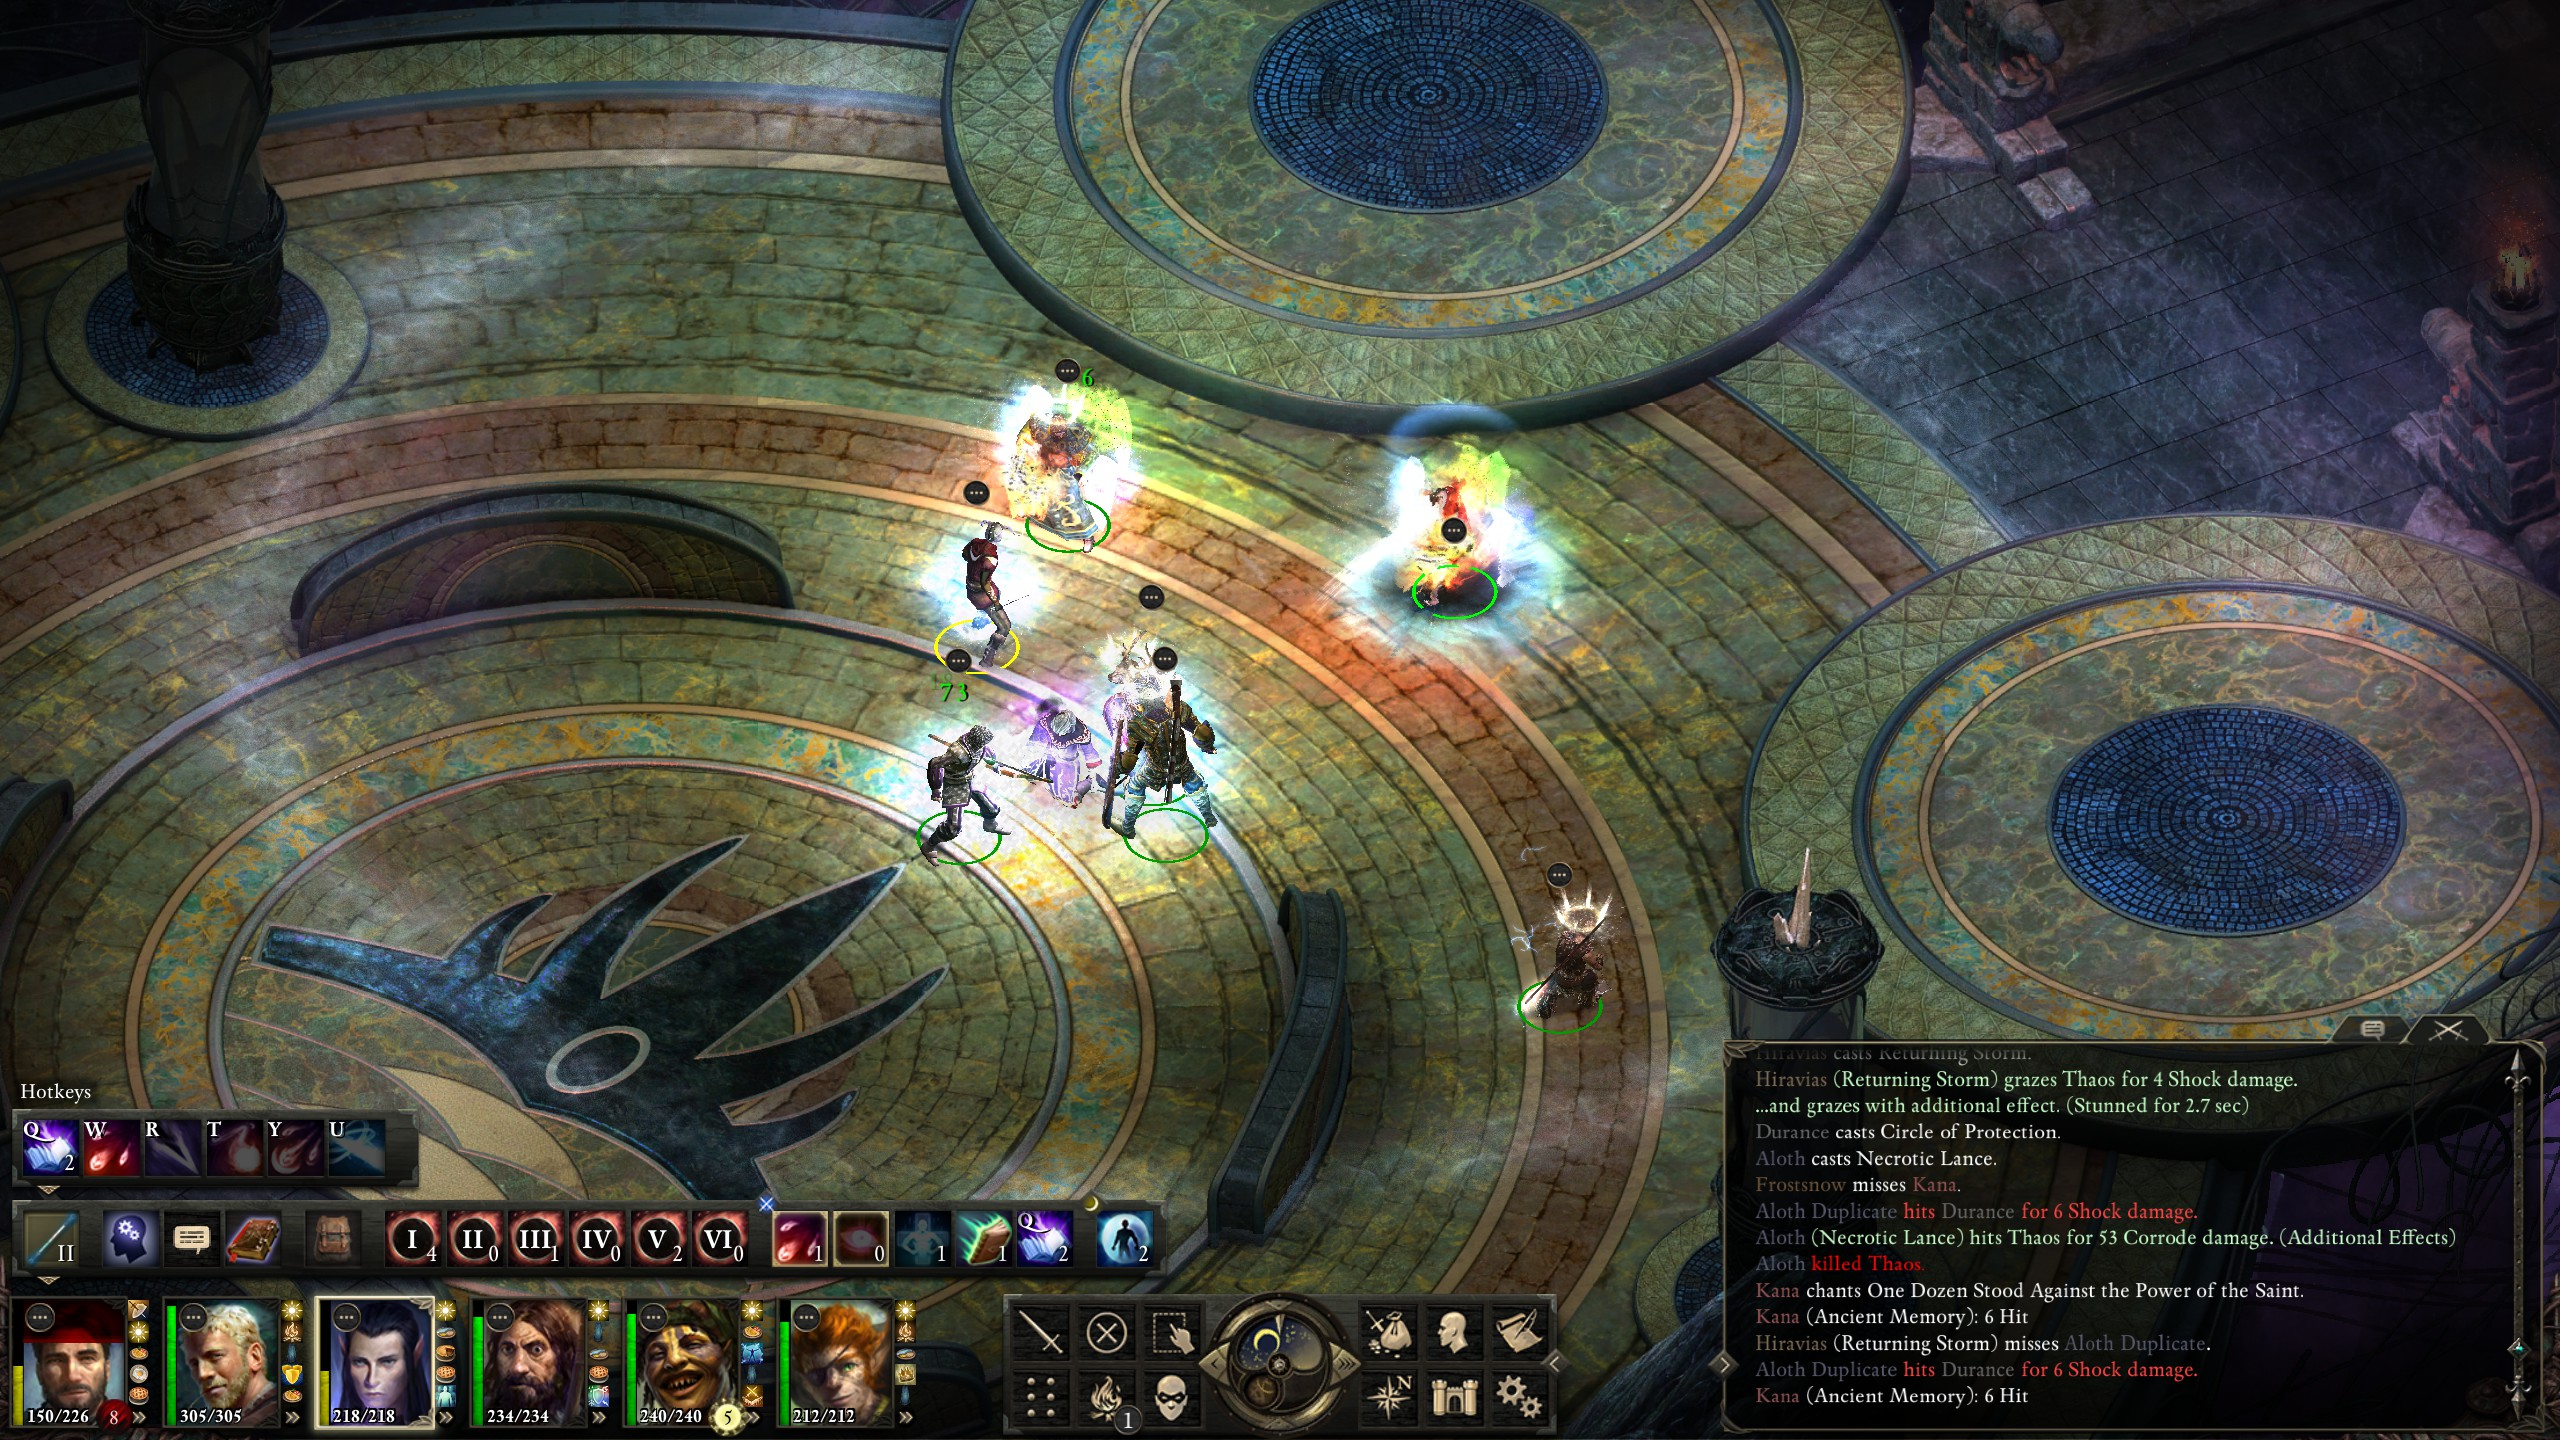
\includegraphics[scale=0.33]{files/blog/2019_03_17_pillars_of_eternity_path_of_the_damned_act_iv/2019_03_17_thaos6.jpg}
\end{figure}

And that was it!  I had beaten the game on the highest difficulty!

\begin{figure}
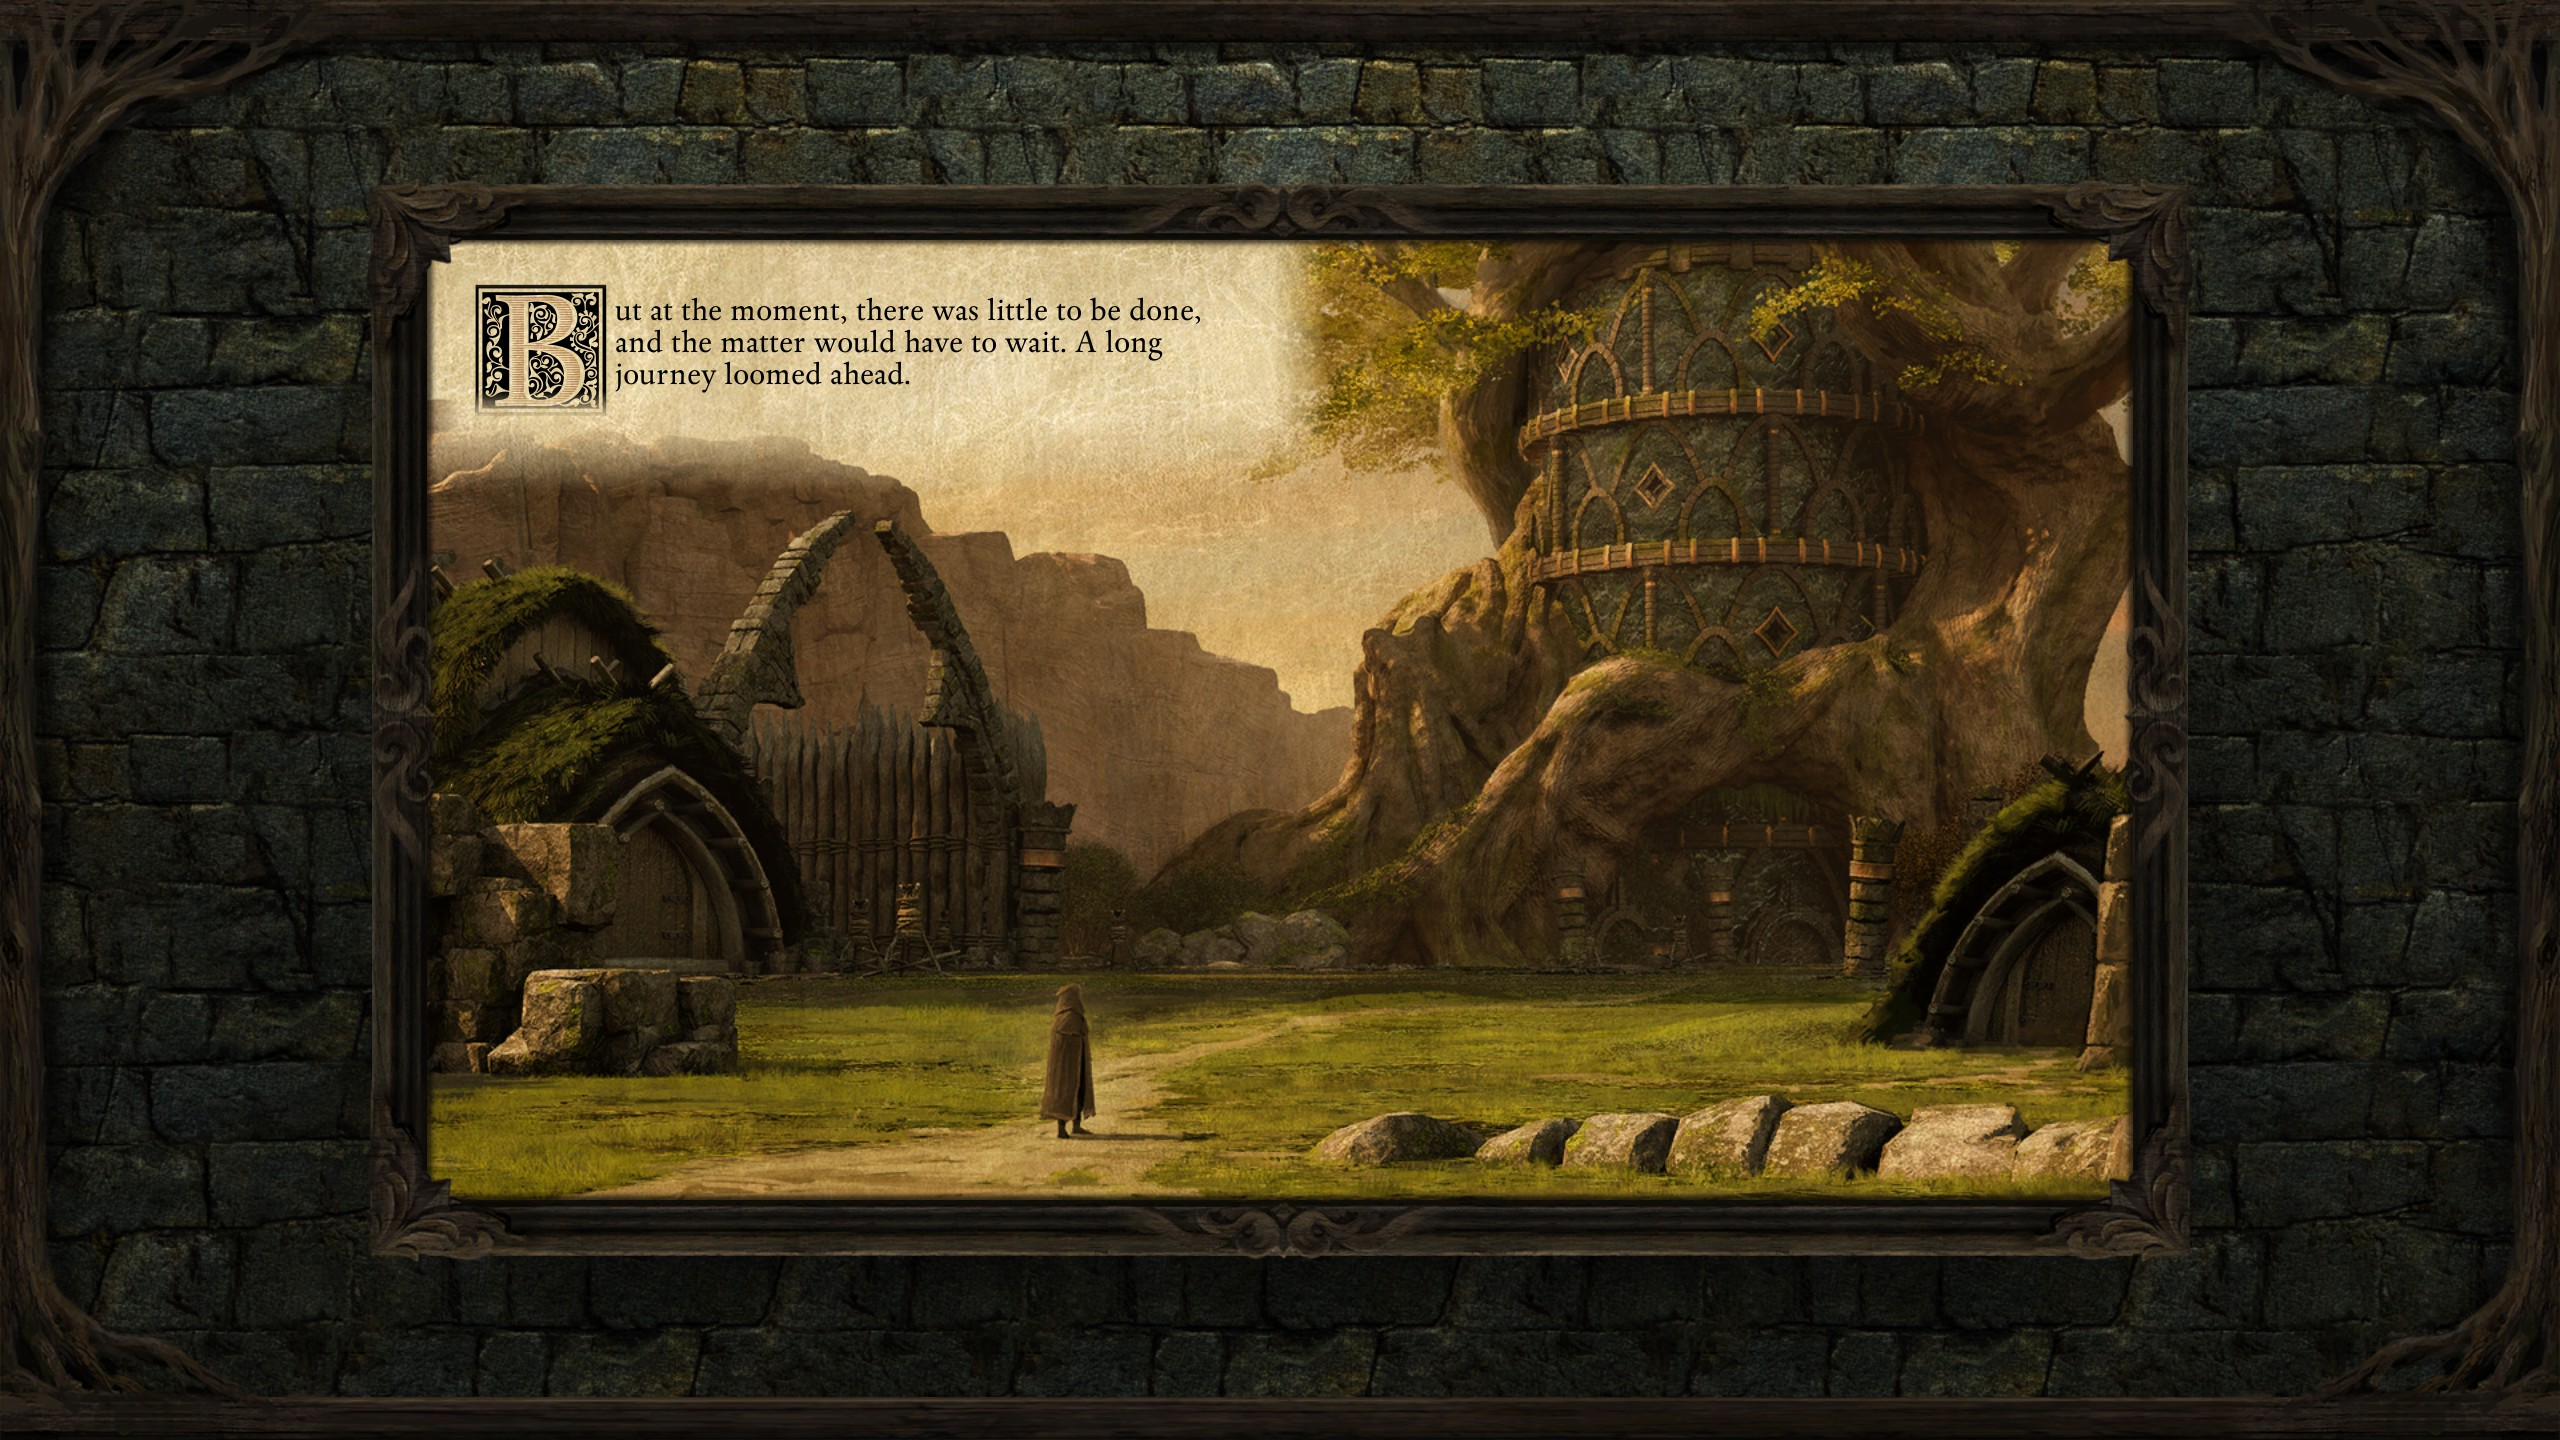
\includegraphics[scale=0.33]{files/blog/2019_03_17_pillars_of_eternity_path_of_the_damned_act_iv/2019_03_17_end.jpg}
\end{figure}

Thinking back on how the run had gone, knowing where to go and how to out-level most areas made the run much easier than it otherwise would have been.  Out-levelling aside, the bosses, especially the Master Below, were still quite difficult, so the run had a good amount of challenge regardless.

The sequel has an option to enable upward-only level-scaling, so that may alleviate the out-levelling advantage I had, but level-scaling doesn't always properly increase the difficulty of lower-level areas (for example, level-scaled mobs often only have their corresponding lower-level status afflictions) or it may mis-compensate and make some creatures ultra-hard at certain levels but not others.  I'll find out eventually, but, for now, there are still the White March expansions that need to be done before I will proceed to the sequel.


% Pillars of Eternity: Path of the Damned, Act III
\section{2019-03-04 Pillars of Eternity: Path of the Damned, Act III}
By this act I'd gotten to the point where the game became easier thanks to my high level.  Continuing the strategy I'd developed earlier worked well, although it wasn't put to any particularly difficult tests in this act.  The game was mostly a matter of staying on top of fights and tossing a few high levels spells out as needed for crowd control.  Thus this blog is more of a visual tour/record of the path I took than any particular strategy employed.

\subsection{To Twin Elms}
The first journey was leaving the riots of Defiance Bay for Twin Elms via Stormwall George.  Rather than go down the path, I decided to explore Lle a Rhemen on my way through.

\begin{figure}
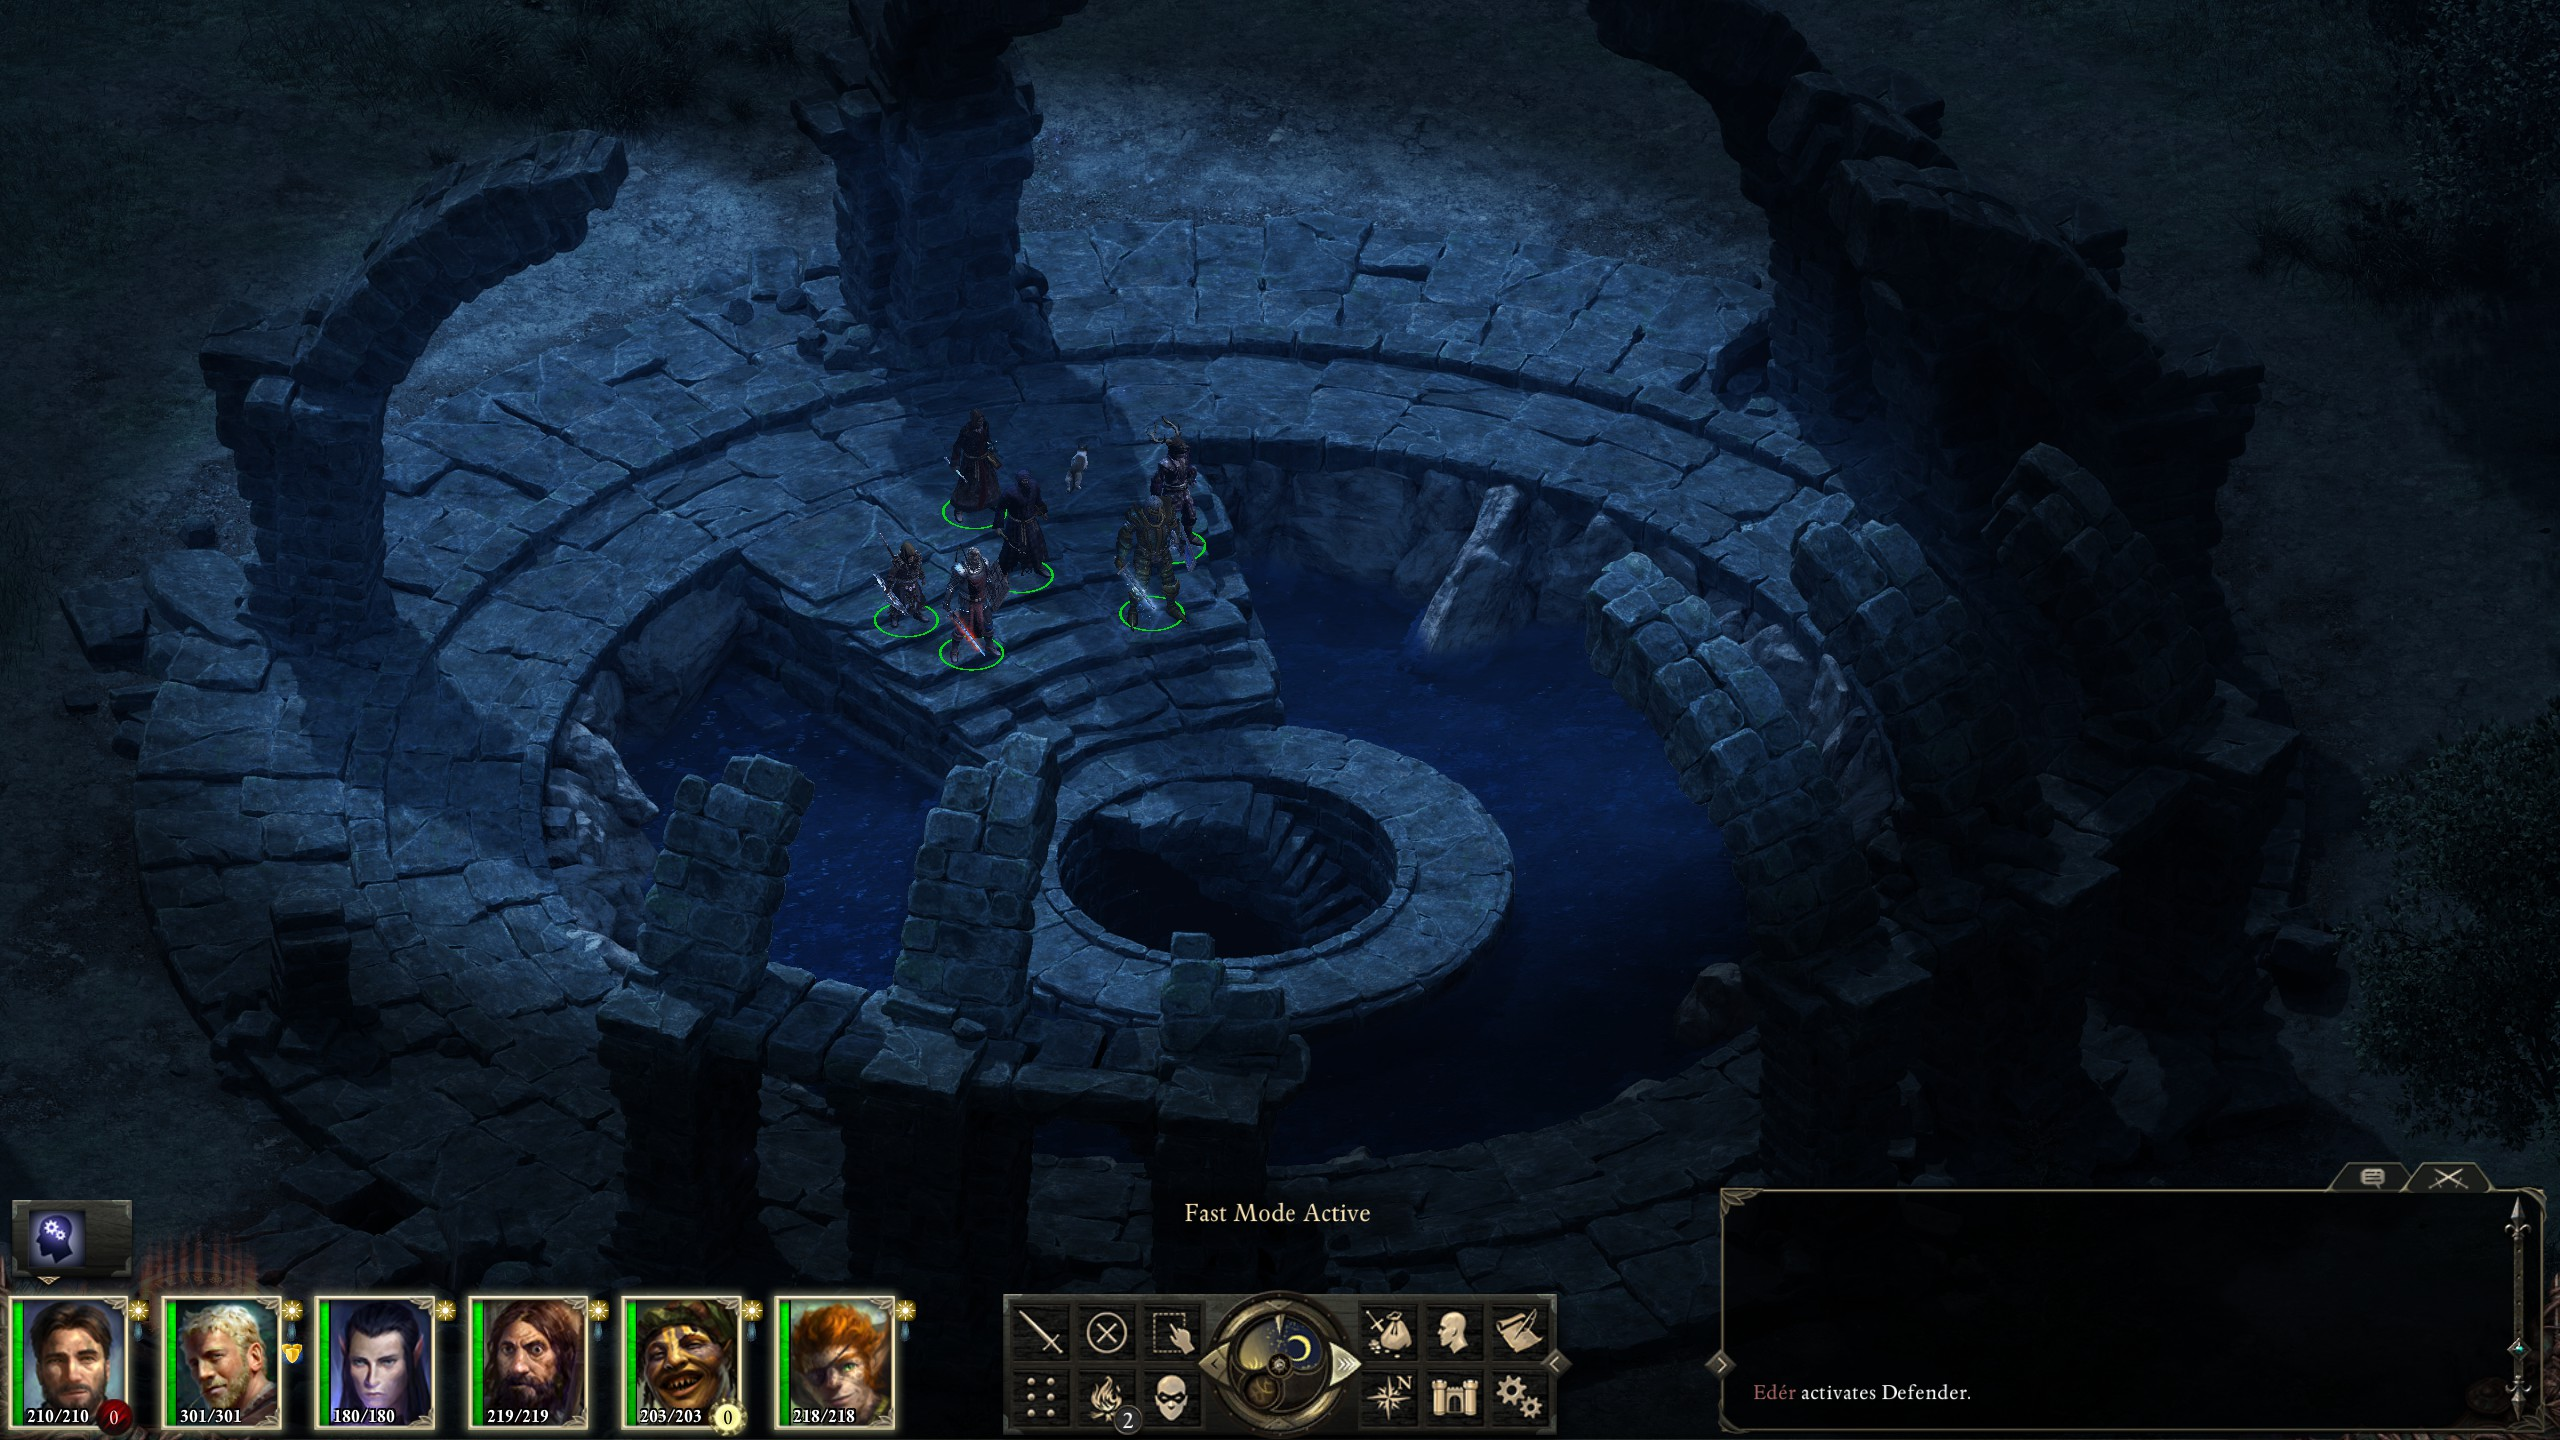
\includegraphics[scale=0.33]{files/blog/2019_03_04_pillars_of_eternity_path_of_the_damned_act_iii/2019_03_04_llearhemen_entrance.jpg}
\end{figure}

The creatures inside were moderately tricky with their freezing pillars; I also made the mistake of sending the monk in alone against one, and he was promptly petrified and knocked out.

\begin{figure}
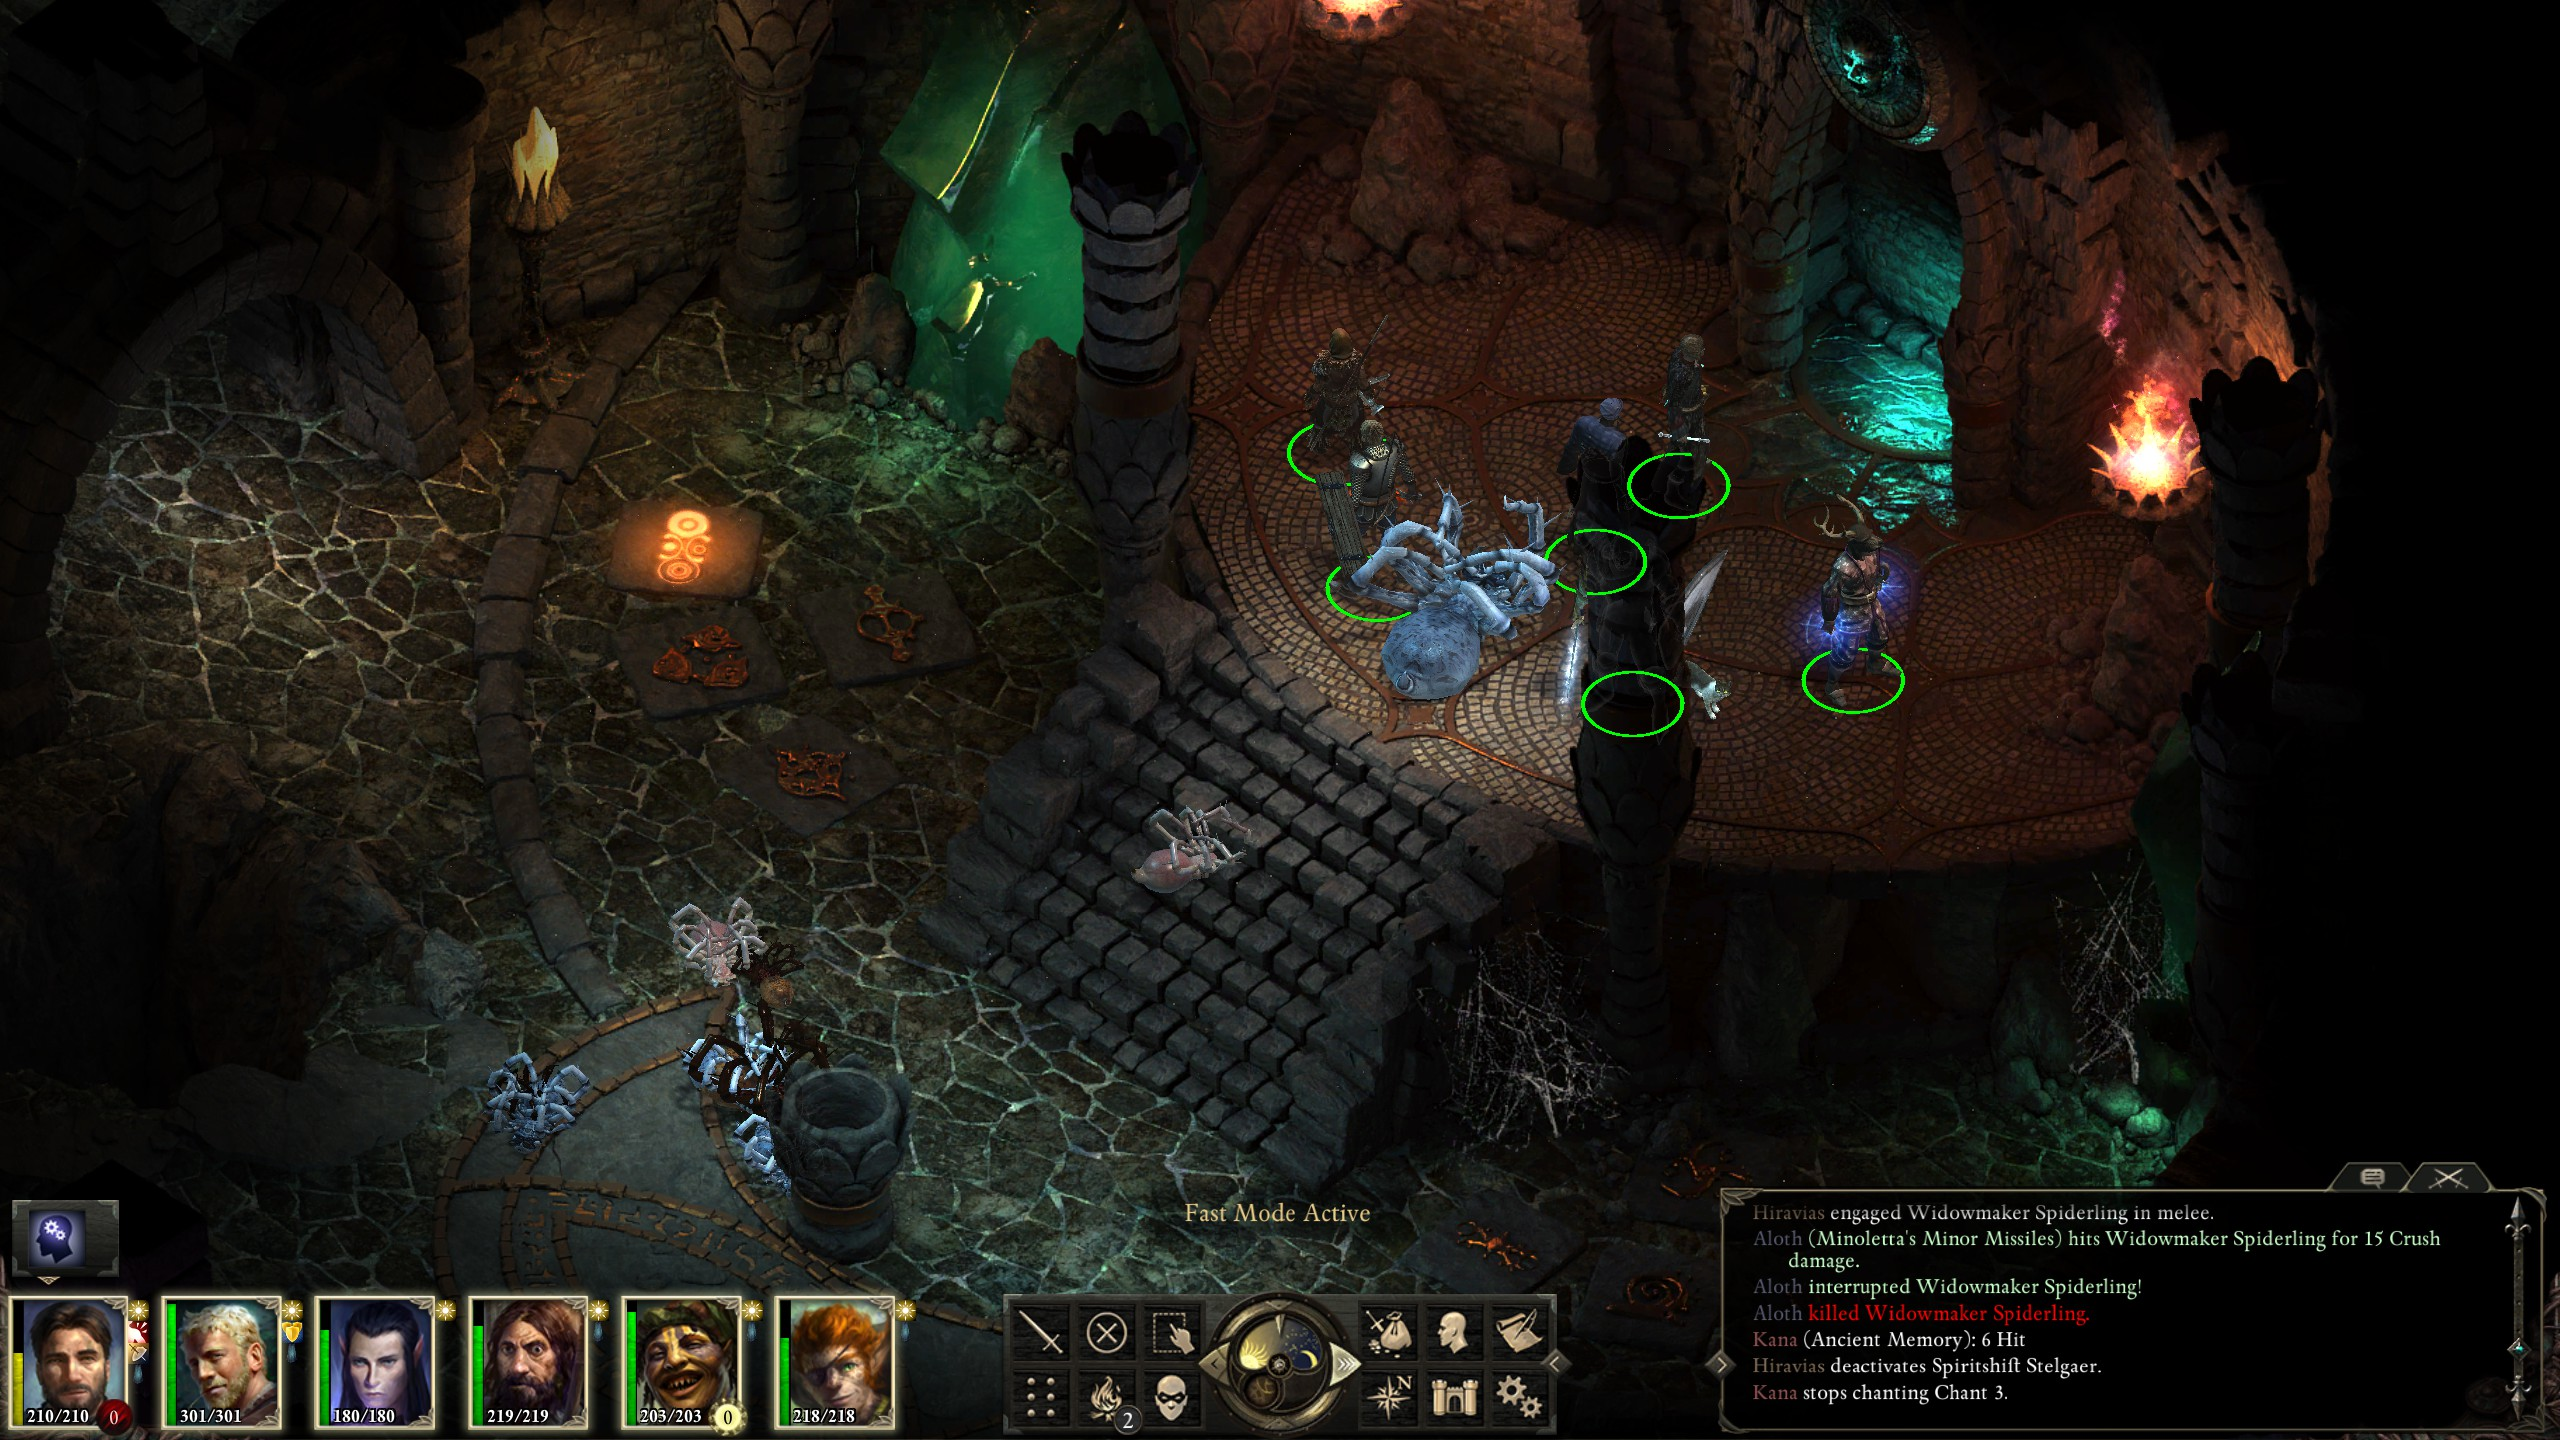
\includegraphics[scale=0.33]{files/blog/2019_03_04_pillars_of_eternity_path_of_the_damned_act_iii/2019_03_04_llearhemen_floor1.jpg}
\end{figure}

The final floor was much easier despite its narrow ledges.

\begin{figure}
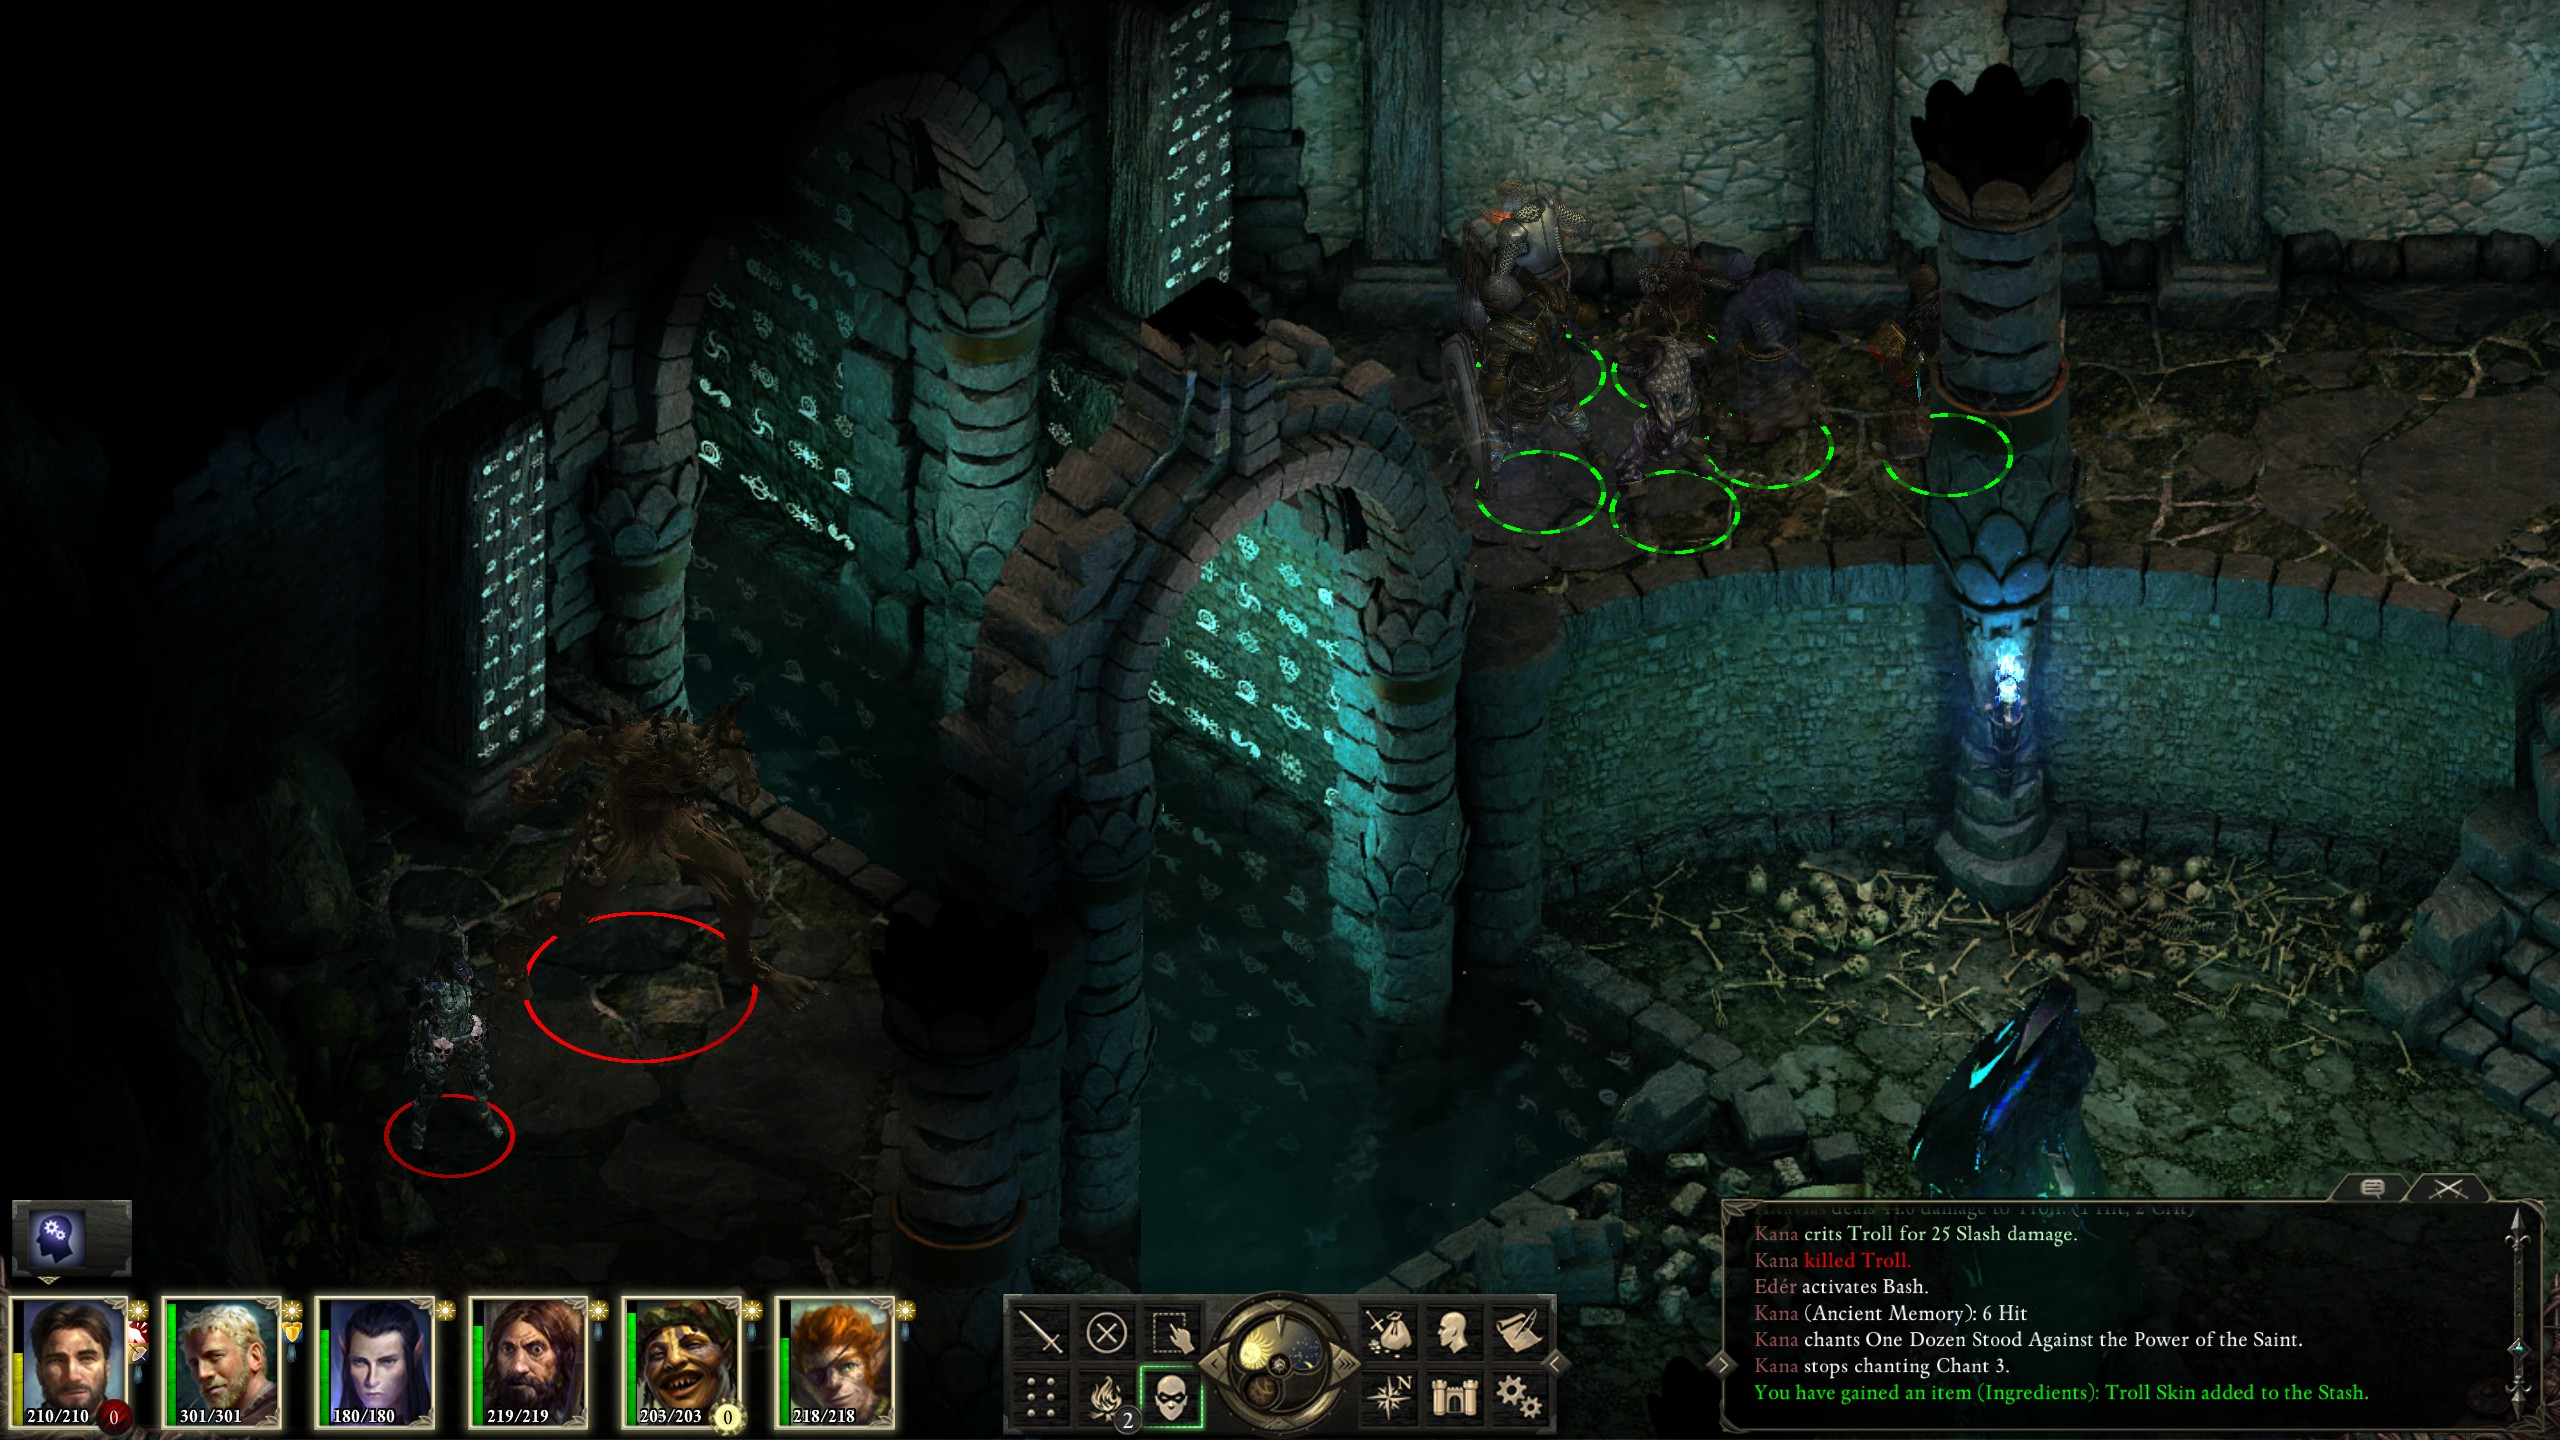
\includegraphics[scale=0.33]{files/blog/2019_03_04_pillars_of_eternity_path_of_the_damned_act_iii/2019_03_04_llearhemen_floor2.jpg}
\end{figure}

Once outside I cleared out the oozes and spores with their annoying confusion and dominate abilities.

\begin{figure}
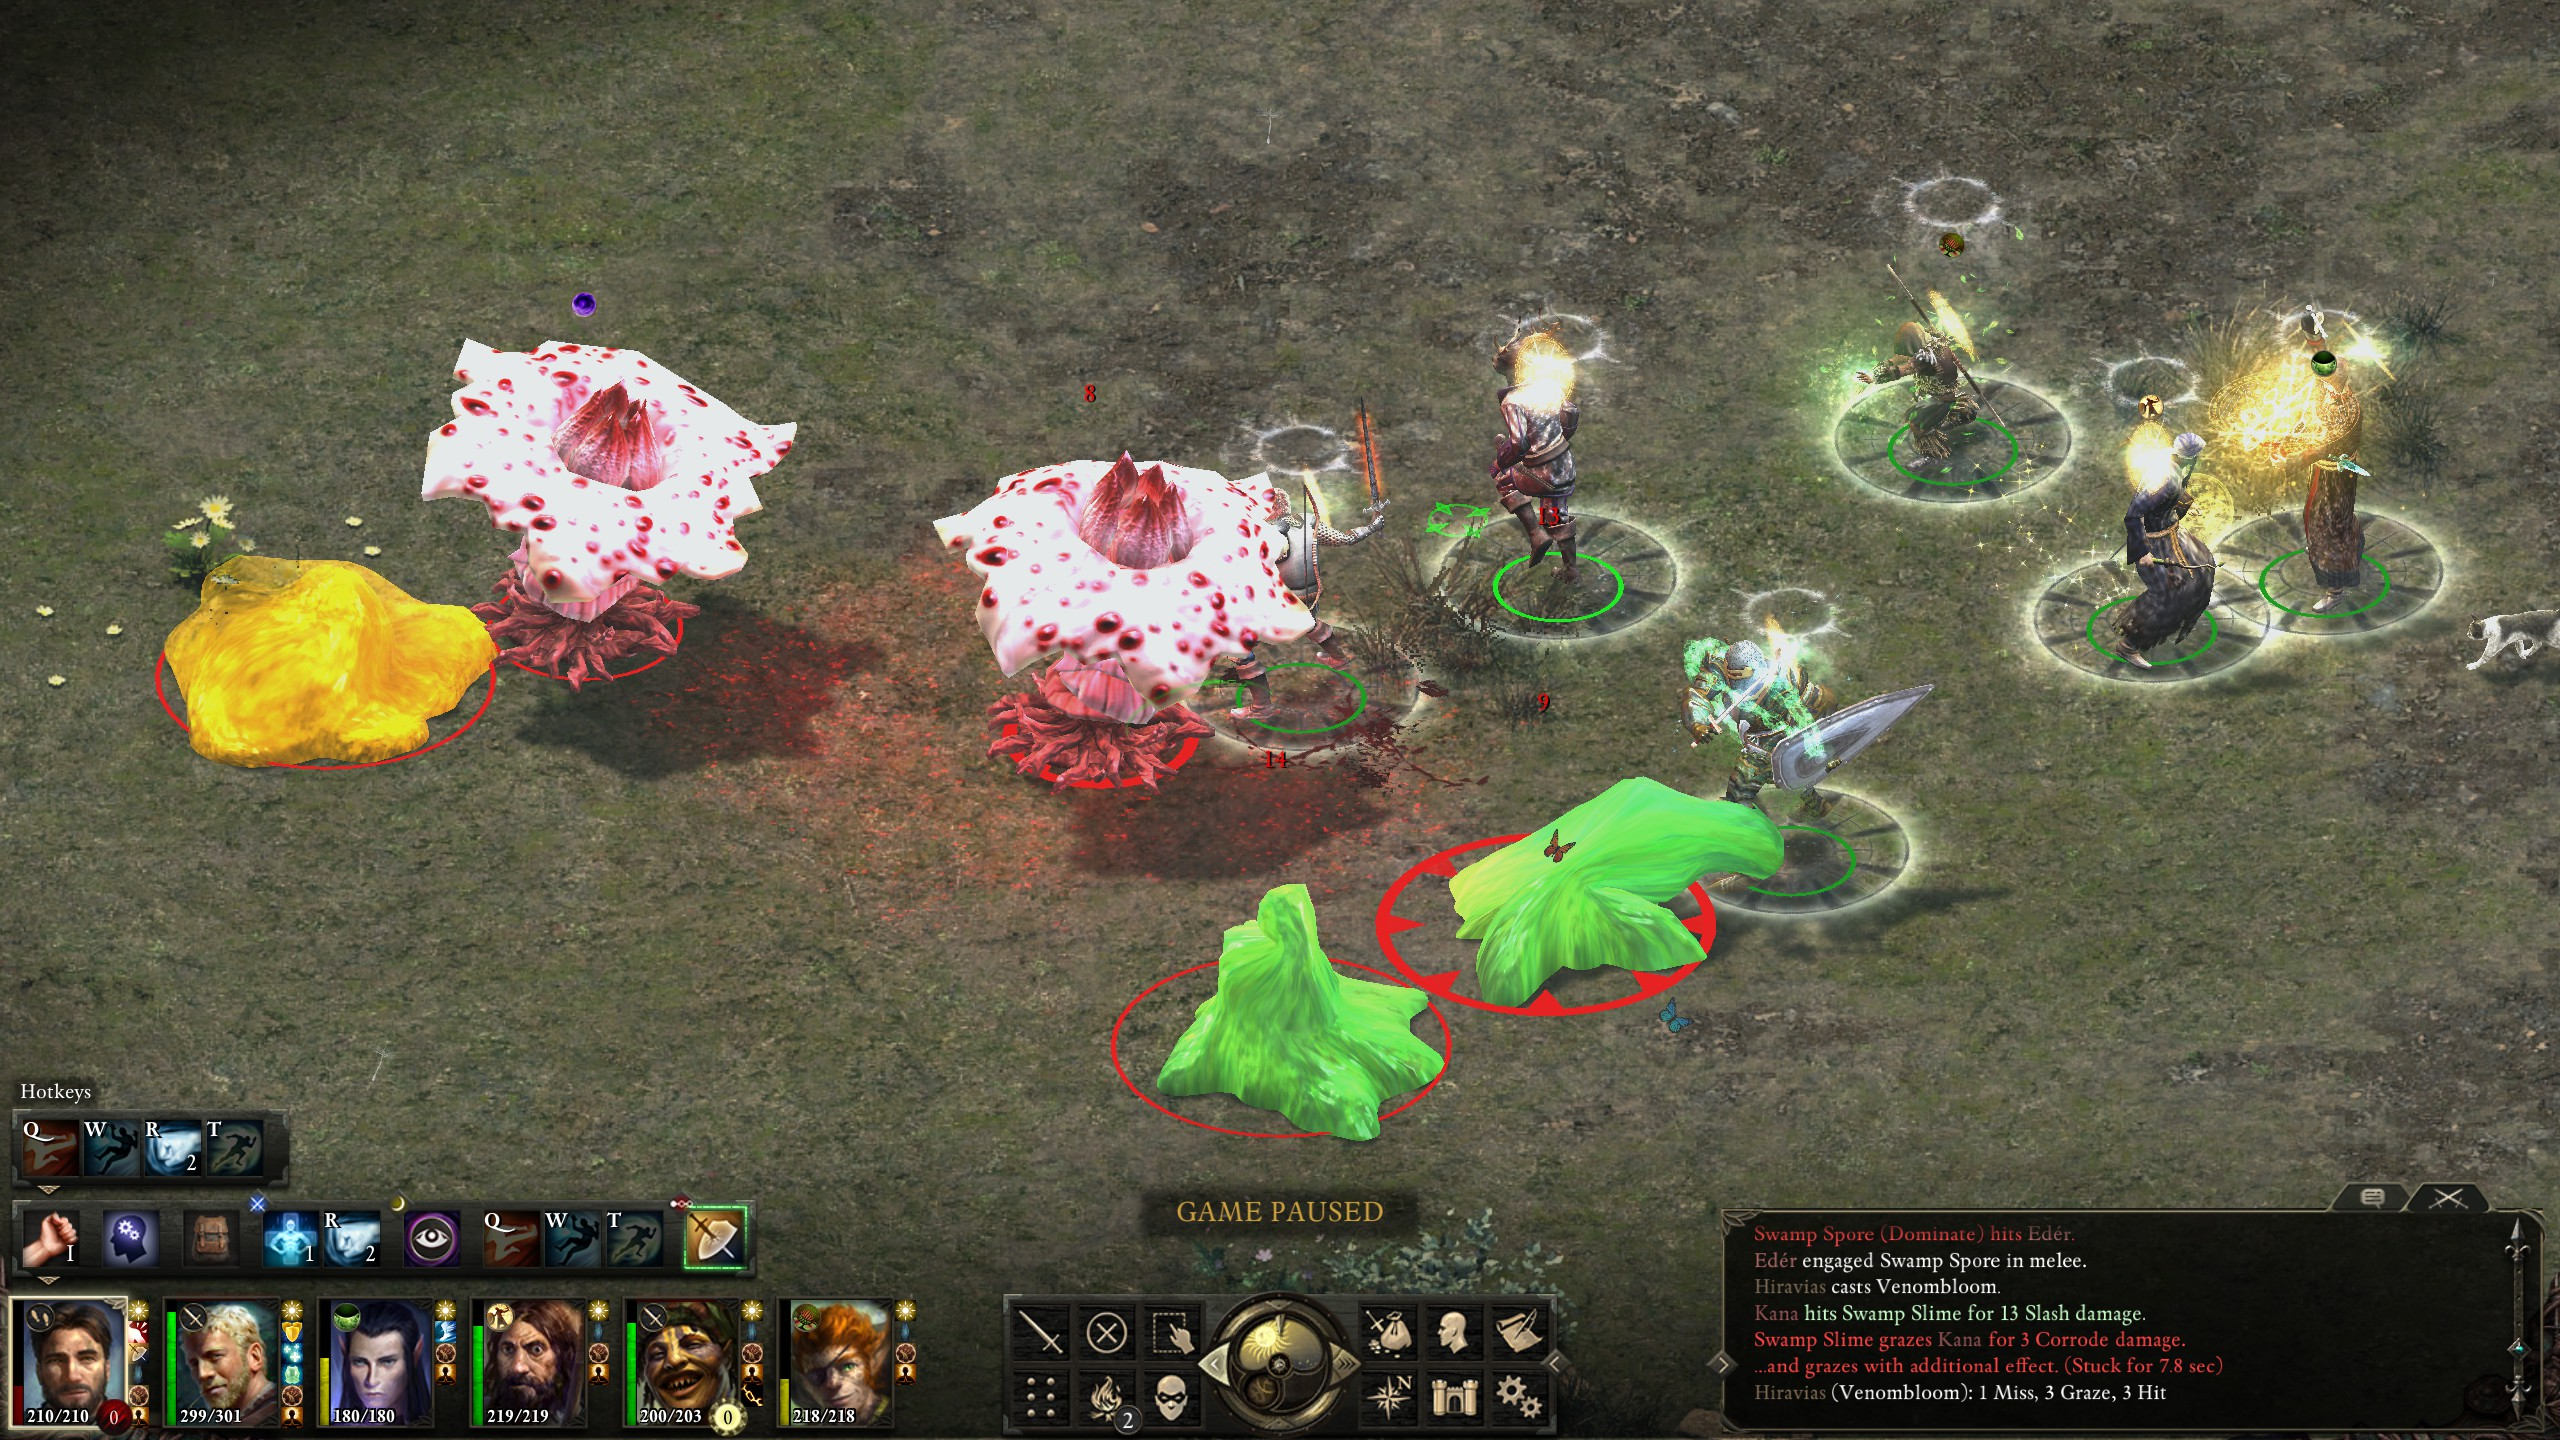
\includegraphics[scale=0.33]{files/blog/2019_03_04_pillars_of_eternity_path_of_the_damned_act_iii/2019_03_04_stormwall.jpg}
\end{figure}

Moving onto Elmshore I received the usual "High Level" challenge (despite not having any of the expansions installed), which I accepted.

\begin{figure}
\includegraphics[scale=0.7]{files/blog/2019_03_04_pillars_of_eternity_path_of_the_damned_act_iii/2019_03_04_highlevel.jpg}
\end{figure}

Elmshore had only a few fights but most of them were decently tough; I also learned that blights, unlike undead, could be rendered unconscious.

\begin{figure}
\includegraphics[scale=0.33]{files/blog/2019_03_04_pillars_of_eternity_path_of_the_damned_act_iii/2019_03_04_elmshore.jpg}
\end{figure}

The way to Twin Elms was then clear.

\begin{figure}
\includegraphics[scale=0.33]{files/blog/2019_03_04_pillars_of_eternity_path_of_the_damned_act_iii/2019_03_04_elmshore2.jpg}
\end{figure}

First, though, it was time to do a few bounties (after clearing the a way to the cave).

\begin{figure}
\includegraphics[scale=0.33]{files/blog/2019_03_04_pillars_of_eternity_path_of_the_damned_act_iii/2019_03_04_elmshore3.jpg}
\end{figure}

\subsection{Bounties}

I made the mistake of trying to pull Nalrend the Wise across a trap; his adds then blasted me with spells while the bears blocked my path\ldots

\begin{figure}
\includegraphics[scale=0.33]{files/blog/2019_03_04_pillars_of_eternity_path_of_the_damned_act_iii/2019_03_04_nalrend1.jpg}
\end{figure}

not that it was enough to save him.

\begin{figure}
\includegraphics[scale=0.33]{files/blog/2019_03_04_pillars_of_eternity_path_of_the_damned_act_iii/2019_03_04_nalrend2.jpg}
\end{figure}

Next up was Thorfen\ldots

\begin{figure}
\includegraphics[scale=0.33]{files/blog/2019_03_04_pillars_of_eternity_path_of_the_damned_act_iii/2019_03_04_thorfen1.jpg}
\end{figure}

Who was easily defeated.

\begin{figure}
\includegraphics[scale=0.33]{files/blog/2019_03_04_pillars_of_eternity_path_of_the_damned_act_iii/2019_03_04_thorfen2.jpg}
\end{figure}

After him came Songsmith Roska.

\begin{figure}
\includegraphics[scale=0.33]{files/blog/2019_03_04_pillars_of_eternity_path_of_the_damned_act_iii/2019_03_04_roska1.jpg}
\end{figure}

Who was also easily crushed (especially by Durance's "Pillar of Holy Fire").

\begin{figure}
\includegraphics[scale=0.33]{files/blog/2019_03_04_pillars_of_eternity_path_of_the_damned_act_iii/2019_03_04_roska2.jpg}
\end{figure}

I made the mistake of getting too close to the ledge when fighting Glasdial\ldots

\begin{figure}
\includegraphics[scale=0.33]{files/blog/2019_03_04_pillars_of_eternity_path_of_the_damned_act_iii/2019_03_04_glasdial1.jpg}
\end{figure}

but made up for it by casting spells from above.

\begin{figure}
\includegraphics[scale=0.33]{files/blog/2019_03_04_pillars_of_eternity_path_of_the_damned_act_iii/2019_03_04_glasdial2.jpg}
\end{figure}

Daroth Grimault, being undead, was immune to the unconscious affliction\ldots

\begin{figure}
\includegraphics[scale=0.33]{files/blog/2019_03_04_pillars_of_eternity_path_of_the_damned_act_iii/2019_03_04_daroth_grimault1.jpg}
\end{figure}

but petrify and stunned still worked.

\begin{figure}
\includegraphics[scale=0.33]{files/blog/2019_03_04_pillars_of_eternity_path_of_the_damned_act_iii/2019_03_04_daroth_grimault2.jpg}
\end{figure}

Captain Muarumi and his crew, however, being regular kith, were not so immune.

\begin{figure}
\includegraphics[scale=0.33]{files/blog/2019_03_04_pillars_of_eternity_path_of_the_damned_act_iii/2019_03_04_captain_muarumi1.jpg}
\end{figure}

"Ninagauth's Freezing Pillar" then demolished them while their reflex saves were low.

\begin{figure}
\includegraphics[scale=0.33]{files/blog/2019_03_04_pillars_of_eternity_path_of_the_damned_act_iii/2019_03_04_captain_muarumi2.jpg}
\end{figure}

I don't even recall the fight with Galen Dalgard\ldots

\begin{figure}
\includegraphics[scale=0.33]{files/blog/2019_03_04_pillars_of_eternity_path_of_the_damned_act_iii/2019_03_04_galen1.jpg}
\end{figure}

but I know that I now use that excellent shield (Old Gerun's Wall) of his!

\begin{figure}
\includegraphics[scale=0.33]{files/blog/2019_03_04_pillars_of_eternity_path_of_the_damned_act_iii/2019_03_04_galen2.jpg}
\end{figure}

Foemyna and her beasts were easily distracted by the summoning trinkets\ldots

\begin{figure}
\includegraphics[scale=0.33]{files/blog/2019_03_04_pillars_of_eternity_path_of_the_damned_act_iii/2019_03_04_foemyna1.jpg}
\end{figure}

Then quickly finished.

\begin{figure}
\includegraphics[scale=0.33]{files/blog/2019_03_04_pillars_of_eternity_path_of_the_damned_act_iii/2019_03_04_foemyna2.jpg}
\end{figure}

The next bounty was up in Northweald, so it and the ones after it would have to wait for me to explore Twin Elms first.

\subsection{Twin Elms}
First up in Twin Elms was the Hearthsong district.  There were no fights in this district but there's a marketplace with another excellent figurine\ldots

\begin{figure}
\includegraphics[scale=0.33]{files/blog/2019_03_04_pillars_of_eternity_path_of_the_damned_act_iii/2019_03_04_hearthsong1.jpg}
\end{figure}

A storyline encounter with the anamenfath\ldots

\begin{figure}
\includegraphics[scale=0.33]{files/blog/2019_03_04_pillars_of_eternity_path_of_the_damned_act_iii/2019_03_04_hearthsong2.jpg}
\end{figure}

And a pretty awesome tree-house inn.

\begin{figure}
\includegraphics[scale=0.33]{files/blog/2019_03_04_pillars_of_eternity_path_of_the_damned_act_iii/2019_03_04_hearthsong3.jpg}
\end{figure}

From Elms' Reach I then went towards Teir Evron.

\begin{figure}
\includegraphics[scale=0.33]{files/blog/2019_03_04_pillars_of_eternity_path_of_the_damned_act_iii/2019_03_04_elmsreach1.jpg}
\end{figure}

Although I took a quick detour in order to deal with the brute Simoc\ldots

\begin{figure}
\includegraphics[scale=0.33]{files/blog/2019_03_04_pillars_of_eternity_path_of_the_damned_act_iii/2019_03_04_elmsreach2.jpg}
\end{figure}

before actually entering Teir Evron.

\begin{figure}
\includegraphics[scale=0.33]{files/blog/2019_03_04_pillars_of_eternity_path_of_the_damned_act_iii/2019_03_04_elmsreach3.jpg}
\end{figure}

Quests in hand I went to Oldsong.

\begin{figure}
\includegraphics[scale=0.33]{files/blog/2019_03_04_pillars_of_eternity_path_of_the_damned_act_iii/2019_03_04_oldsong1.jpg}
\end{figure}

While doing the Maw I accidentally agro'd another group of enemies, then ran straight into a "Gaze of the Adragan" trap which almost took me out, though I managed to recover and win the fight.

\begin{figure}
\includegraphics[scale=0.33]{files/blog/2019_03_04_pillars_of_eternity_path_of_the_damned_act_iii/2019_03_04_oldsong2.jpg}
\end{figure}

Not learning from my previous mistakes I took on a group in Rymrgand's temple while low on spells\ldots

\begin{figure}
\includegraphics[scale=0.33]{files/blog/2019_03_04_pillars_of_eternity_path_of_the_damned_act_iii/2019_03_04_oldsong3.jpg}
\end{figure}

Only to have a patrol open the door and bring another wave of enemies in.

\begin{figure}
\includegraphics[scale=0.33]{files/blog/2019_03_04_pillars_of_eternity_path_of_the_damned_act_iii/2019_03_04_oldsong4.jpg}
\end{figure}

I managed to survive again, but the ordeal was more dangerous than I'd have liked.

\begin{figure}
\includegraphics[scale=0.33]{files/blog/2019_03_04_pillars_of_eternity_path_of_the_damned_act_iii/2019_03_04_oldsong5.jpg}
\end{figure}

Setbacks aside, after Twin Elms was clear it was onto Northweald for quests, including a bounty and a dragon!

\subsection{Northweald}

The wilderness of Northweald is quite pretty, though it has its fair share of monsters.

\begin{figure}
\includegraphics[scale=0.33]{files/blog/2019_03_04_pillars_of_eternity_path_of_the_damned_act_iii/2019_03_04_northweald01.jpg}
\end{figure}

In the northern cave I found the next bounty: Devwen and her druids.

\begin{figure}
\includegraphics[scale=0.33]{files/blog/2019_03_04_pillars_of_eternity_path_of_the_damned_act_iii/2019_03_04_northweald02.jpg}
\end{figure}

They didn't stand a chance.

\begin{figure}
\includegraphics[scale=0.33]{files/blog/2019_03_04_pillars_of_eternity_path_of_the_damned_act_iii/2019_03_04_northweald03.jpg}
\end{figure}

Up the stairs, however, to Hylea's Temple was where the real fun lay, though, for there was the Sky Dragon!  I began the fight by using the summoning trinkets in order to eat up the "Returning Storm" spells of the wind blights, then focused the blights as best I could.

\begin{figure}
\includegraphics[scale=0.33]{files/blog/2019_03_04_pillars_of_eternity_path_of_the_damned_act_iii/2019_03_04_northweald04.jpg}
\end{figure}

Eder then got rather unlucky against a breath attack\ldots

\begin{figure}
\includegraphics[scale=0.33]{files/blog/2019_03_04_pillars_of_eternity_path_of_the_damned_act_iii/2019_03_04_northweald05.jpg}
\end{figure}

but I managed to recover and finish off the blights.

\begin{figure}
\includegraphics[scale=0.33]{files/blog/2019_03_04_pillars_of_eternity_path_of_the_damned_act_iii/2019_03_04_northweald06.jpg}
\end{figure}

Luck decided to favor me next, as Aloth managed to land a "Gaze of the Adragan" on the dragon.

\begin{figure}
\includegraphics[scale=0.33]{files/blog/2019_03_04_pillars_of_eternity_path_of_the_damned_act_iii/2019_03_04_northweald07.jpg}
\end{figure}

I used the opportunity to unlesh everything I could on it: Durance's "Pillar of Holy Fire", Hiravas' "Sunlance", and Aloth's "Minoletta's Concussive Missiles".

\begin{figure}
\includegraphics[scale=0.33]{files/blog/2019_03_04_pillars_of_eternity_path_of_the_damned_act_iii/2019_03_04_northweald08.jpg}
\end{figure}

The volley didn't outright kill the dragon, but it took it most of the way down, and it wasn't long after that I won the fight.

\begin{figure}
\includegraphics[scale=0.33]{files/blog/2019_03_04_pillars_of_eternity_path_of_the_damned_act_iii/2019_03_04_northweald09.jpg}
\end{figure}

With the dragon dead and the bounty done I was ready to head to Burial Isle, but first it was time to show a certain tyrant that he should have stayed dead.

\subsection{Undead Raedric}

As blackberry vines cut but not pulled up from the root soon sprout stems anew, so Raedric rose as a death knight.

\begin{figure}
\includegraphics[scale=0.33]{files/blog/2019_03_04_pillars_of_eternity_path_of_the_damned_act_iii/2019_03_04_raedric1.jpg}
\end{figure}

The trick to this fight was to mitigate the fampyrs' dominate afflictions by using Durance's "Prayer Against Treachery" on the party, disregarding the "Fireball" thrown by Raedric.

\begin{figure}
\includegraphics[scale=0.33]{files/blog/2019_03_04_pillars_of_eternity_path_of_the_damned_act_iii/2019_03_04_raedric2.jpg}
\end{figure}

With their powerful affliction impotent, the fampyrs then became merely tough undead.  Some skilled nuking then quickly dispatched both them and Raedric.

\begin{figure}
\includegraphics[scale=0.33]{files/blog/2019_03_04_pillars_of_eternity_path_of_the_damned_act_iii/2019_03_04_raedric3.jpg}
\end{figure}

With that thug down it was then time to finish cleaning up the remaining ruffians in the Dyrwood.

\subsection{Final Bounties}

The first of the final three bounties was Naroc the Prophet.

\begin{figure}
\includegraphics[scale=0.33]{files/blog/2019_03_04_pillars_of_eternity_path_of_the_damned_act_iii/2019_03_04_naroc1.jpg}
\end{figure}

The fight had some difficulties as his barbarians seemed able to chain cast "Heart of Fury", but I managed to pull through.

\begin{figure}
\includegraphics[scale=0.33]{files/blog/2019_03_04_pillars_of_eternity_path_of_the_damned_act_iii/2019_03_04_naroc2.jpg}
\end{figure}

Hiding in the ruins of previously-explored Teir Nowneth was Ysly\ldots

\begin{figure}
\includegraphics[scale=0.33]{files/blog/2019_03_04_pillars_of_eternity_path_of_the_damned_act_iii/2019_03_04_ysly1.jpg}
\end{figure}

who did not prove to be as much of a challenge as the previous bounty.

\begin{figure}
\includegraphics[scale=0.33]{files/blog/2019_03_04_pillars_of_eternity_path_of_the_damned_act_iii/2019_03_04_ysly2.jpg}
\end{figure}

Last and most difficult was Lord Exarch Sserkal.

\begin{figure}
\includegraphics[scale=0.33]{files/blog/2019_03_04_pillars_of_eternity_path_of_the_damned_act_iii/2019_03_04_sserkal1.jpg}
\end{figure}

What makes this fight so difficult is the massive amount of crowd control used by him and his cronies.  Their "Psychic Blast" spell stuns, and in addition they have a confusion.  I had used "Prayer Against Treachery" in the belief that they had dominates and charms, but did not bank on having nearly my entire team confused.

\begin{figure}
\includegraphics[scale=0.33]{files/blog/2019_03_04_pillars_of_eternity_path_of_the_damned_act_iii/2019_03_04_sserkal2.jpg}
\end{figure}

Despite the odds I managed to have Aloth kite and petrify the foes long enough to take a couple out (it helps that they are low health), then Durance's confusion wore off and he was able to cast "Crowns for the Faithful" on a few of my team members for the extra will saves.  After that I was able to turn the fight around.

\begin{figure}
\includegraphics[scale=0.33]{files/blog/2019_03_04_pillars_of_eternity_path_of_the_damned_act_iii/2019_03_04_sserkal3.jpg}
\end{figure}

Despite the fight's difficulty, the "Gwisk Glas" won was well worth the effort.

Bounties done, I headed back to Twin Elms' Burial Isle.

\subsection{Burial Isle}

The isle itself was full of high-level spirits, especially Cean Gwla, making Durance's "Prayer Against Imprisonment" extremely useful.  After a bit of fighting, I finally stood above Woedica's pit.

\begin{figure}
\includegraphics[scale=0.33]{files/blog/2019_03_04_pillars_of_eternity_path_of_the_damned_act_iii/2019_03_04_burialisle.jpg}
\end{figure}

The pit beckoned me onto Act IV, but it would have to wait until the next blog, of course.


% Rebuilding a Mathematical Foundation: Euclid, Books I to V
\section{2019-02-21 Rebuilding a Mathematical Foundation: Euclid, Books I to V}
Since leaving college for the workforce, the amount of math I've had to do has been reduced to nothing.  While some might welcome this, I find it rather tragic as, to me, math is an incredibly useful tool that allows me to recognize abstract patterns in complex situations and thus get a grasp on things that would otherwise be overwhelming or elude comprehension.  Instead I learn things such as the specifics of Application Programming Interfaces (APIs) and how to use specific Graphical User Interfaces (GUIs), but, as instances of a class are ephemeral, so are specific APIs and GUIs to their underlying mathematical patterns (to the extent that the patterns are understood), and I'd prefer to get a better handle on the underlying patterns than constantly running the rat-race of memorizing specifics.

I took some time to remedy this on my own by trying to \htmladdnormallink{self-study}{https://github.com/clinew/introduction_to_algorithms} out of \htmladdnormallink{Rivest, et al.}{https://en.wikipedia.org/wiki/Introduction_to_Algorithms}, but while trying to do so I found that the mathematical foundation that I'd retained from my academic years was lacking.  Some of that could be blamed on the academic institutions, as not all of my teachers were great and inspiring, while other times it could be blamed on myself, as I tended to put more thought into women than mathematical truth during my teenage years.  Regardless of how I'd gotten there it became clear to me that I needed some kind of refresher in order to fill in the gaps left by my teachers and me, which meant I had to come up with some kind of plan.

\subsection{Developing a Plan}
I began by doing some \htmladdnormallink{serious academic research}{https://www.wikipedia.org} with an emphasis on the type mathematics most relevant to computers, focusing on names of theoreticians that I already knew of such as Turing, Von Neumann, and Church.  From this I compiled a list of authors and potential works that seemed relevant to a solid mathematical foundation with an emphasis on computation, coupled with a couple other possibly interesting works; alas it was not always clear from the Wikipedia page which works would be relevant nor were they always enumerated in a clear manner, but the list which I compiled was a rough start:
\begin{itemize}
	\item George Boole
	\begin{itemize}
		\item The Mathematical Analysis of Logic
		\item An Investigation of the Laws of Thought
	\end{itemize}
	\item Augustus De Morgan
	\begin{itemize}
		\item Trigonometry and Double Algebra
		\item Formal Logic
		\item Budget of Paradoxes
		\item Relations
	\end{itemize}
	\item Von Neumann
	\begin{itemize}
		\item Mathematical Foundations of Quantum Mechanics
		\item Theory of Games and Economic Behaviour
		\item "The Mathematician"
		\item Theory of Self Reproducing Automata
		\item On the Introduction of Transfinite Numbers
		\item An Axiomization of Set Theory
		\item The General and Logical Theory of Automata
		\item Continuous Geometry
	\end{itemize}
	\item Alan Turing
	\begin{itemize}
		\item Collected Works of A. M. Turing
	\end{itemize}
	\item Alonzo Church
	\begin{itemize}
		\item Church's Theorem (Entscheidungsproblem)
		\item Church-Turing Thesis
		\item Introduction to Mathematical Logic
		\item The Calculi of Lambda-Conversion
		\item A Bibliography of Symbolic Logic
		\item Logic, Meaning and Computation: Essays in memory of Alonzo Church
	\end{itemize}
	\item Claude Shannon
	\begin{itemize}
		\item A Symbolic Analysis of Relay and Switching Circuits
		\item The Mathematical Theory of Communication
		\item Communication Theory of Secrecy Systems
		\item Claude Elwood Shannon: Collected Papers (IEEE Press)
		\item Programming a Computer for Playing Chess
	\end{itemize}
	\item Gottfried Wilhelm Leibniz
	\begin{itemize}
		\item Monadologie
		\item A Philosopher's Creed
		\item General Inqueries About the Analysis and Concepts of Truth
		\item Explanation of Binary Arithmetic
		\item New Essays on Human Understanding
	\end{itemize}
	\item Isaac Newton
	\begin{itemize}
		\item Mathematical Principles of Natural Philosophy
		\item Opticks
		\item Method of Fluxions
	\end{itemize}
	\item Euclid of Alexandria
	\begin{itemize}
		\item Elements
	\end{itemize}
	\item Aristotle
	\begin{itemize}
		\item Organon
	\end{itemize}
	\item Pythagoras of Samos
	\item Georg Cantor
	\begin{itemize}
		\item On a Property of the Collection of All Real Algebraic Numbers
		\item Contributions to the Founding of the Theory of Transfinite Numbers
	\end{itemize}
	\item Bertrand Russel
	\begin{itemize}
		\item The Principles of Mathematics
		\item Principa Mathematica
		\item Logical Atomism
	\end{itemize}
	\item Kurt Godel
	\begin{itemize}
		\item Godel's Completeness Theorem
		\item On Formally Undecidable Propositions of "Principa Mathematica" and Related Systems
		\item Consistency of the axiom of choice and of the generalized continuum-hypothesis with the axioms of set theory
	\end{itemize}
	\item Haskell Curry
	\begin{itemize}
		\item Foundations of Mathematical Logic
		\item Combinatory Logic
		\item A theory of formal deducibility
	\end{itemize}
\end{itemize}
This was quite the list (note that Pythagoras of Samos had no writings to study!), so obviously some kind of order would have to be imposed on it.  The first thing was to realize that it'd be too much to read all of each author's works, so the best bet would be to try and pick one or two of each author's best, most influential, and most relevant works to read.  Next, some kind of structure should be imposed on the order of readings; as knowledge tends to build upon itself, a chronological order seemed most natural here, but with the later authors it was unclear who should come first, therefore I gave them a tentative grouping and order.  The list, with their groups, was thus as follows:
\begin{itemize}
	\item "Ancients"
	\begin{itemize}
		\item Euclid's Elements
		\item Aristotle's Organon
		\item Newton's Mathematical Principles of Natural Philosophy
		\item Leibniz's Explanation of Binary Arithmetic
	\end{itemize}
	\item Computers
	\begin{itemize}
		\item George Boole
		\begin{itemize}
			\item The Mathematical Analysis of Logic
			\item An Investigation of the Laws of Thought
		\end{itemize}
		\item Augustus De Morgan
		\begin{itemize}
			\item Formal Logic
			\item Budget of Paradoxes
		\end{itemize}
		\item Von Neumann
		\begin{itemize}
			\item "The Mathematician"
			\item Theory of Self Reproducing Automata
			\item The General and Logical Theory of Automata
		\end{itemize}
		\item Alan Turing
		\begin{itemize}
			\item Collected Works of A. M. Turing
		\end{itemize}
		\item Alonzo Church
		\begin{itemize}
			\item Church's Theorem (Entscheidungsproblem)
			\item Church-Turing Thesis
			\item Introduction to Mathematical Logic
		\end{itemize}
		\item Claude Shannon
		\begin{itemize}
			\item A Symbolic Analysis of Relay and Switching Circuits
			\item The Mathematical Theory of Communication
			\item Communication Theory of Secrecy Systems
		\end{itemize}
	\end{itemize}
	\item Others
	\begin{itemize}
		\item Georg Cantor
		\begin{itemize}
			\item On a Property of the Collection of All Real Algebraic Numbers
		\end{itemize}
		\item Bertrand Russel
		\begin{itemize}
			\item The Principles of Mathematics
			\item Principa Mathematica
		\end{itemize}
		\item Von Neumann
		\begin{itemize}
			\item An Axiomization of Set Theory (Von Neumann-Bernays-Godel set theory) (Russel's paradox first)
		\end{itemize}
		\item Kurt Godel
		\begin{itemize}
			\item Godel's Completeness Theorem (The completeness of the axioms of the functional calculus of logic)
			\item Godel's Incompleteness Theorem (On Formally Undecidable Propositions of "Principa Mathematica" and Related Systems)
		\end{itemize}
		\item Haskell Curry
		\begin{itemize}
			\item Foundations of Combinatorial Logic
			\item Foundations of Mathematical Logic
		\end{itemize}
	\end{itemize}
\end{itemize}
This list gave a rough outline for how to proceed; though it's likely far from perfect, I won't be able to fully realize how until later.  I'll likely end up splicing in a few works from the "Others" category as I progress, depending on what seems appropriate.  It's also a highly-ambitious project that will likely take me decades to complete given full-time employment and my hobby projects, but I imagine it will be worthwhile, even if I do manage to complete the project.  The basic plan in place, it was thus time to begin, starting nearly two and half millennia ago with Euclid's "Elements".

\subsection{Euclid, Books I to V}
When I began reading Euclid it wasn't exactly clear to me whether I'd have anything worth saying, in fact, I'm still not convinced that I do, as I've no doubt that many highly-educated mathematical scholars have made extensive commentary of the text, whereas I am a mere computer programmer taking a cursory read through it.  As such, I will not even try giving any kind of comprehensive commentary and will instead point out a few things that I found befuddling, interesting, or otherwise noteworthy, after quickly providing the details of my methodology.

The translation that I chose to read was Thomas L. Heath's translation.  Given my current time-management system it would have been impractical to tackle all of "Elements" in one go, thus I divvied it up into four sections: 1) books I to V, 2) books VI - IX, 3) book X, and 4) books XI - XIII.  As you may have surmised from the title, this blog covers only the first section.

The material of these first five books felt in many ways like a refresher of high school geometry, except without the sleep-inducing monotone of my teacher that year.  However, the material also felt more mature, like a college course; as I recall, fewer things were proven in high school and more was asserted, this created a more disjoint effect than Euclid, who started with a few simple premises and then continuously built upon them.  As with most books, the language has taken a bit of getting used to; the algebraic form of math which I am accustomed to was likely not developed when "Elements" was written, but the diagrams with every proposition more than made up for the unfamiliar vernacular.

\subsubsection{Book I, Proposition 7}
The first major difficulty that I ran into was in \htmladdnormallink{Book I, Proposition 7}{https://mathcs.clarku.edu/~djoyce/java/elements/bookI/propI7.html}, which had the following diagram and statement:
\begin{center}
\begin{figure}
\begin{makeimage}
\fbox{ % I don't like this but haven't fixed latex2html's cropping bug yet.
\begin{tikzpicture}
	\coordinate [label=left:A] (A) at (0, 0);
	\coordinate [label=right:B] (B) at (10, 0);
	\coordinate [label=above:C] (C) at (7, 4);
	\coordinate [label=right:D] (D) at (9, 3);
	\draw (A) -- (B);
	\draw (A) -- (C);
	\draw (A) -- (D);
	\draw (B) -- (C);
	\draw (B) -- (D);
	\draw (C) -- (D);
\end{tikzpicture}
}
\end{makeimage}
\end{figure}
\end{center}
\begin{quote}
Thus, since \textit{AC} is equal to \textit{AD},
\begin{centering}
the angle \textit{ACD} is also equal to the angle \textit{ADC}; \\
therefore the angle \textit{ADC} is greater than the angle \textit{DCB}; \\
therefore the angle \textit{CDB} is much greater than the angle \textit{DCB}. \\
\end{centering}
\end{quote}

What wasn't clear to me was how, exactly, \textit{ADC} was bigger than \textit{DCB}.  The answer in this case was the unstated assumption that "the part is greater than the whole"; looking at the diagram I was supposed to have noticed how the angle \textit{DCB} was within the angle \textit{ACD}, therefore \textit{DCB} was less than \textit{ACD} and, since \textit{ADC} was proven equal to \textit{ACD}, \textit{DCB} was thus also less than \textit{ADC}.  This confused me because, at this point, I was not yet sure whether to treat the diagram as part of the proposition and thus containing information perhaps not explicitly stated or as an auxiliary piece of information to help visualize the proposition.  Given the proposition so far, one could construct an alternate diagram as follows:
\begin{center}
\begin{figure}
\begin{makeimage}
\fbox{
\begin{tikzpicture}
	\coordinate [label=left:A] (A) at (0, 0);
	\coordinate [label=right:B] (B) at (10, 0);
	\coordinate [label=above:C] (C) at (3, 4);
	\coordinate [label=left:D] (D) at (1, 3);
	\draw (A) -- (B);
	\draw (A) -- (C);
	\draw (A) -- (D);
	\draw (B) -- (C);
	\draw (B) -- (D);
	\draw (C) -- (D);
\end{tikzpicture}
}
\end{makeimage}
\end{figure}
\end{center}
In this case the angle \textit{ADC} would be less than the angle \textit{DCB} (at least, given the proposition so far, as the whole thing is proved absurd in the end).  Thus it was impossible to come to either conclusion regarding \textit{ADC} and \textit{DCB} without the extra information contained in the diagram.  Once it became apparent that the diagram contained information not explicitly stated in the text the proposition became readily understandable.  While it may seem trivial, this misunderstanding caused me untold confusion for a few hours as I had to map out both possibilities to the end while constantly mentally-switching between the two, unsure which one to progress.

\subsubsection{Book I, Proposition 47}
Perhaps this was shown me long ago, perhaps not; this proposition is a proof of the Pythagorean Theorem.  It was interesting to see as, despite being able to use the theorem in calculations, I had not thought to visualize it as literal squares on the side of the triangle, nor that I could reason about the relationship of their sizes based on the geometry I'd learned.
\begin{center}
\begin{figure}
\begin{makeimage}
\fbox{
\begin{tikzpicture}
	\coordinate [label=225:B] (B) at (0, 0);
	\coordinate [label=right:C] (C) at (5, 0);
	\coordinate [label={[label distance=1mm,above]105:A}] (A) at (53.13014723127149049863:3);
	\path (B) +(0, -5) coordinate [label=below left:D] (D);
	\path (D) +(5, 0) coordinate [label=below right:E] (E);
	\path (A) +(143.13014723127149049863:3) coordinate [label=above:G] (G);
	\path (G) +(233.13014723127149049863:3) coordinate [label=left:F] (F);
	\path (A) +(53.13014723127149049863:4) coordinate [label=above:H] (H);
	\path (H) +(323.13014723127149049863:4) coordinate [label=right:K] (K);
	\draw (A) -- (B) -- (C) -- (A);
	\draw (B) -- (D) -- (E) -- (C) -- (B);
	\draw (A) -- (G) -- (F) -- (B);
	\draw (A) -- (H) -- (K) -- (C);
	\draw (A) -- (D);
	\draw (A) -- (E);
	\draw (C) -- (F);
	\draw (B) -- (K);
	\draw (A) -- (A |- D) coordinate [label=below:L] (L);
\end{tikzpicture}
}
\end{makeimage}
\end{figure}
\end{center}
I won't re-iterate the formula here as it's easily searchable.

\subsubsection{Book III, Proposition 16}
This was the first time I'd ever really heard the term "rectilineal angle" used, and I found it quite baffling:
\begin{center}
\begin{figure}
\begin{makeimage}
\fbox{
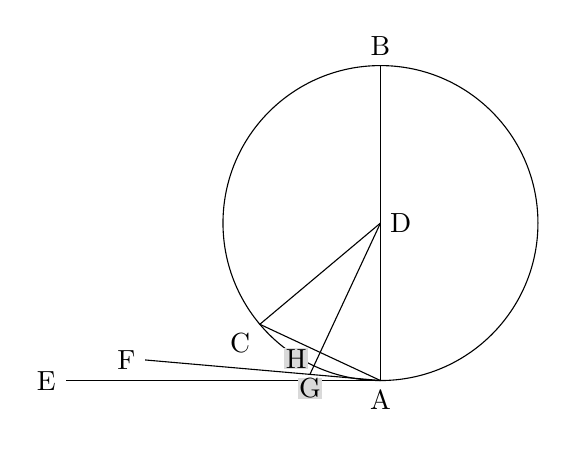
\begin{tikzpicture}
	\definecolor{mycolor}{RGB}{217, 217, 217}; % Designed LaTeX2HTML transparency color.
	\coordinate [label=above:B] (B) at (0, 2);
	\coordinate [label=below:A] (A) at (0, -2);
	\coordinate [label=right:D] (D) at (0, 0);
	\coordinate [label=below left:C] (C) at (220:2);
	\coordinate [label=left:E] (E) at (-4, -2);
	\path (0, -2) +(175:3) coordinate [label=left:F] (F);
	\draw (0, 0) circle [radius=2];
	\draw (B) -- (A) -- (E);
	\draw (D) -- (C) -- (A);
	\draw [name path=af] (A) -- (F);
	\path [name path=dh] (D) -- (245:3);
	\draw [name intersections={of=af and dh}] (D) -- (intersection-1) coordinate [label={[label distance=1pt,fill=mycolor,inner sep=0.5pt]below:G}] (G);
	\coordinate [label={[label distance=2pt,fill=mycolor,inner sep=0.5pt,anchor=335]165:H}] (H) at (245:2);
\end{tikzpicture}
}
\end{makeimage}
\end{figure}
\end{center}
\begin{quote}
I say further that the angle of the semicircle contained by the straight line \textit{BA} and the circumference \textit{CHA} is greater than any acute rectilineal angle, and the remaining angle contained by the circumference \textit{CHA} and the straight line \textit{AE} is less than any acute rectilineal angle.
\end{quote}

Not sure what Euclid meant by "the angle contained by\ldots the circumference \textit{CHA}", I tried imagining the segment \textit{CHA} and thus the angle contained by the line \textit{CA} and \textit{BA} or \textit{AE}, but that didn't make any sense.  After thinking on the text a bit longer I gave up and decided to search for the proposition and landed at \htmladdnormallink{this page}{https://mathcs.clarku.edu/~djoyce/java/elements/bookIII/propIII16.html} (whose site I'd come across earlier) which explained that what Euclid was referring to was called a "Horn angle"; that is, Euclid was describing the angle made between a \emph{line} and a \emph{curve}.  Nothing that I'd learned in geometry had prepared me for this; I'd always thought of angles as between straight lines, never between curves, hence I was totally blind-sided by the idea.  The proposition now made sense, though, and I was lucky enough to not have to consider horn angles for the rest of my reading (so far).

\subsection{Epilogue: Generating a Transparent Graph}
The last graph took a surprising amount of effort in order to generate, so I'm going to ramble about it here.  The trick came about in part because of the \textit{G} and \textit{H} labels; unlike the other labels, these needed to mask the lines under them.  The simple solution was to add a \texttt{fill=white} command, but, of course this doesn't quite work on the grayish background of the webpage, but, wait, what's with that background:
\begin{figure}
\includegraphics[scale=0.5]{files/blog/2019_02_21_math_euclid_pt1/2019_02_21_broken.png}
\caption{Figure is produced with a contrasting background.}
\end{figure}
Though I could change the fill to the same color as the webpage background, I didn't know what color that was and worried that future graphs may need more colors that would trigger this issue, so I resolved to find out what was going on and fix it.

I first supplied \texttt{-debug} to the \texttt{latex2html} command-line and learned that the final part of the image processing involves running the \texttt{pnmcrop}, \texttt{ppmquant}, and then \texttt{pnmtopng} commands.  Unfortunately, \LaTeX2html was cleaning the intermediate PNM, PS, and PNG files, but that was remedied by editing the \texttt{latex2html} file's \texttt{cleanup} function to simply return rather than perform clean-up.  Looking at the intermediate files I then noticed that all of the PostScript and PNM files in fact had the same gray background, it was only the PNG images in which the background had (usually) become fully transparent.  For example, here is how the graph relating to Book I, Proposition 47 looks like as a PNM (though it was converted to a PNG for posting's sake):
\begin{figure}
\includegraphics[scale=0.5]{files/blog/2019_02_21_math_euclid_pt1/2019_02_21_workspnm.png}
\caption{PNMs of images that work fine have the same gray background.}
\end{figure}
Looking closer at the commands showed that the \texttt{-trans '#d9d9d9'} option was being passed to \texttt{pnmtopng}, thus it seemed that the gray color was being used as a marker for what would become transparent in the final PNG image, but why wasn't it working for this problem image?  I also took a look at the resulting files with the \texttt{file} command, naming one image "working" and the other "broken" after whether they rendered as per my expectation or not, respectively:
\begin{quote}
\begin{verbatim}
	works.pnm:  Netpbm image data, size = 1032 x 1093, rawbits, pixmap
	broken.pnm: Netpbm image data, size = 643 x 518, rawbits, pixmap
	works.png:  PNG image data, 1032 x 1093, 4-bit colormap, interlaced
	broken.png: PNG image data, 643 x 518, 8-bit grayscale, interlaced
\end{verbatim}
\end{quote}
So the broken image was being converted to a grayscale which had no alpha channel!  I ran the command myself (\texttt{pnmtopng -interlace -trans '#d9d9d9'}) in order to see if I could reproduce the output and, sure enough, ran into the same issue.  I checked the man page for a workaround and noticed that by default the program would use a "nearby" color if the specified transparency color wasn't found, but I could append an \texttt{=} to the color in order to make it match exactly.  When I tried this neither the working image nor the broken image had \emph{any} transparency, and the previously-working image printed the warning \texttt{pnmtopng: specified transparent color not present in palette; ignoring -transparent} as well (the broken image did not print anything); strange that it should only warn for working image, presumably the broken one matched better, but then where was the transparency?!  I figured it must not exist in grayscale images, as they must not have an alpha channel.  At this point I decided to e-mail the soon-to-be-unfortunate program maintainer telling him that I'd run into a bug.  In the meantime I figured out that I could set the fill color with \verb+\definecolor{mycolor}{RGB}{192, 192, 192}+ to make it the same gray as the background and thus cause it to appear transparent as the other, "working", image was, but this workaround was still not satisfying.

The maintainer got back to me and told me that, in fact, the grayscale image does have transparency in it!  Apparently, for images where a single color is designated as transparent, that information is encoded via something called a "\htmladdnormallink{tRNS chunk}{http://www.libpng.org/pub/png/book/chapter08.html#png.ch08.div.5.2}" rather than a separate alpha channel (thus saving space).  He told me that I could check using either \texttt{pngtopam -verbose > /dev/null} or \texttt{pngcheck -v}.  Doing so showed the following:
\begin{quote}
\begin{verbatim}
	File: broken.png (9153 bytes)
	  chunk IHDR at offset 0x0000c, length 13
	    643 x 518 image, 8-bit grayscale, interlaced
	  chunk tRNS at offset 0x00025, length 2
	    gray = 0x00d9
	  chunk IDAT at offset 0x00033, length 8192
	    zlib: deflated, 32K window, default compression
	    rows per pass: 65, 65, 65, 130, 129, 259, 259
	  chunk IDAT at offset 0x0203f, length 878
	  chunk IEND at offset 0x023b9, length 0
	No errors detected in broken.png (5 chunks, 97.3% compression).

	File: works.png (21851 bytes)
	  chunk IHDR at offset 0x0000c, length 13
	    1032 x 1093 image, 4-bit palette, interlaced
	  chunk PLTE at offset 0x00025, length 48: 16 palette entries
	  chunk IDAT at offset 0x00061, length 8192
	    zlib: deflated, 32K window, default compression
	    rows per pass: 137, 137, 137, 274, 273, 547, 546
	  chunk IDAT at offset 0x0206d, length 8192
	  chunk IDAT at offset 0x04079, length 5326
	  chunk IEND at offset 0x05553, length 0
	No errors detected in works.png (6 chunks, 96.1% compression).
\end{verbatim}
\end{quote}
So the broken image did indeed have a transparency value encoded as a tRNS chunk while the working image had a palette entry to designate transparency, but why wasn't it showing as transparent on the broken image?  Were all the image viewers that I tried just buggy?

Then it occurred to me: does \texttt{#d9d9d9} actually map onto an 8-bit grayscale?  I opened the PNG image and noticed that the gray was actually \texttt{#c0c0c0}!  So it had been downscaled, but, wait, it turned out to be the same value in the PNM image... and the PostScript image!  Well, what created the PostScript image?  That turned out to be a DVI file which contained \emph{all} of the images, so it was a bit tricker to analyze.  After digging in \LaTeX2html's source code though I eventually found that the background color was set via the variable \texttt{\$LATEX_COLOR} which was by default \verb+\pagecolor[gray]{.7}+.  By setting this value myself in \texttt{.latex2html-init} to the expected transparency value with \verb+\pagecolor[RGB]{217, 217, 217}+ (the decimal equivalent of the hexadecimal value) and adjusting my workaround to also use said value (never mind that I didn't previously comprehend that I was using \texttt{#c0c0c0} rather than \texttt{#d9d9d9} when I first implemented the workaround) I could then generate a correct image!  In addition, the warning that came from generating a PNG from the PNM file when using the exact transparency specification went away.  Turns out the other images \emph{happened} to work because \texttt{pnmtopng} was selecting the nearby color \texttt{#c0c0c0} when it couldn't find \texttt{#d9d9d9}, but this nearness selection didn't happen when generating a grayscale image, thus causing my problem!

The problem root caused and solution found, I decided to check if there was anywhere I could submit a patch against \LaTeX2html.  Checking my distribution's upstream it appeared that someone had actually taken on maintaining the \htmladdnormallink{program}{https://github.com/latex2html/latex2html/} to some extent, as the original author, Nikos Drakos, was no longer maintaining it.  Before submitting a patch I took a look at the newest version and noticed that a number of significant changes had been made, such as using \texttt{pdflatex} in order to generate images by default.  Slightly daunted, I tried it out, but the results that I got had a black background for all images and made some other changes to the layout of the webpage that I was not particularly keen on.  I tried tweaking the options based on a few of the commits but quickly ran out of patience; I was not trying to port my website to a new version of the tool with breaking changes \emph{and} fix a bug, especially as I'd already dumped so much time into it already.  Before quitting, though, I did notice a \htmladdnormallink{patch}{https://github.com/latex2html/latex2html/commit/02aca89d8c282a8c65d60fcbdd3c6ccf30f4bea8} which appeared to address a similar issue.  Fair enough then, it seemed the problem was already noticed and had a solution; too bad I didn't see it sooner!

Thus the great image conversion transparency saga of early 2019 came to an end.  Hopefully my next blog attempt will run into fewer issues, sheesh!

My thanks to the Netpbm (\texttt{pnmtopng}) maintainer Bryan Henderson for his assistance.


% Pillars of Eternity: Path of the Damned, Act II
\section{2018-11-25 Pillars of Eternity: Path of the Damned, Act II}
At last, part II is done!  The sequel continues to tempt me, but I remain committed to mastering the first game before moving onto the second.

Act II is probably the lengthiest act in the game, consisting of the entire city of Defiance Bay, a journey through the wilderness, Dyrford Village, Engwithian Ruins, and, optionally, most of the Endless Paths; hence in part why it took so long to complete.  That, and work, as I am, alas, not yet retired.

\subsection{Defiance Bay Sidequests}
The first time I entered Defiance Bay the city was rather overwhelming for my completionist nature; how was I to explore every nook and cranny and complete all of the quests?  Talking to a quest-giver often gave quests that lead me to another district, which would quickly tangle me up in a web of half-explored and half-completed areas.  Instead I came up with the following algorithm: explore an entire district, completing all quests that stay within it and other previously-explored areas, then enter a new district and repeat the previous step.  Before completing any quests, however, the first order of business was to grab the awesome summoning trinkets.  The first, "Oaken Scarab Figurine", which summons 3 Wood Beetles, was in a hidden stash near the amphitheatre.  Next, I stole the "Obsidian Lamp Figurine", which summons 3 Shades, from the Vailian Embassy (I would have bought it but they don't offer that option!).  The "Ashwood Cameo Figurine" was being sold by the merchant Lora in the Copperlane merchant district for 15,000 copper; I didn't have the cash to buy it right away, so it had to wait until later.

Figurines in hand, it was time to begin questing.  I went through Copperlane, First Fires, Brackenbury, Ondra's Gift, then finally Heritage Hill.  Since I had gone so deep into the Endless Paths and gained powerful loot and experience, I began to move ahead of the level difficulty, making the journey much easier.  More loot was to come, though; upon completing the first quest for the Crucible Knights (the one that doesn't exclude you from the other factions), I noticed that the smith, Dunstan, sold a pair of boots called "Shod-in-Faith" that would proc "Consecrated Ground" when the wearer was hit by a critical hit.  Since my Monk was having difficulties staying alive, I placed these on my Monk and, when combined with "Fulvano's Amulet", which increases healing received by 25\%, they are insanely powerful, allowing my Monk to profit from damage while not getting beaten down by it.  Further questing in Heritage Hill also gave me the "Iridescent Scarab Figurine", which summons an Adra Beetle, from the family tomb where Saeda was hiding.  The biggest challenge was the lighthouse in Ondra's Gift, but it was nothing an army of figurines couldn't handle:

\begin{figure}
\includegraphics[scale=0.33]{files/blog/2018_11_25_pillars_of_eternity_path_of_the_damned_act_ii/2018_11_25_lighthouse.jpg}
\end{figure}

Amusingly enough, accidentally killing my summoned animat with the adra beetle's "Shocking Blast" gave a little bit of experience.  Having cleared out most of Defiance Bay it was time to progress the main questline a little.

\subsection{Defiance Bay Catacombs}
The catacombs were easy-going as well; I cleared them out without a problem.

\begin{figure}
\includegraphics[scale=0.33]{files/blog/2018_11_25_pillars_of_eternity_path_of_the_damned_act_ii/2018_11_25_catacombs.jpg}
\end{figure}

Having cleared most of Defiance Bay and gained a few levels I next went to dispatch a few ruffians on the road.

\subsection{Bounties}
I find the bounties quite enjoyable.  They are fights where one can go all-out without feeling like they are cheesing it, and, if there's one thing that Pillars is all about, it's epic battles.  First up, the Dweller:

\begin{figure}
\includegraphics[scale=0.33]{files/blog/2018_11_25_pillars_of_eternity_path_of_the_damned_act_ii/2018_11_25_dweller_begin.jpg}
\end{figure}

I began playing around with Aloth's "Minor Grimoire Imprint", but have generally found it too buggy in that it often doesn't actually steal spells when it should.  Regardless, the Dweller went down without much hassle:

\begin{figure}
\includegraphics[scale=0.33]{files/blog/2018_11_25_pillars_of_eternity_path_of_the_damned_act_ii/2018_11_25_dweller_end.jpg}
\end{figure}

Next up was Sly Cidrel.  The battle started out easy enough.

\begin{figure}
\includegraphics[scale=0.33]{files/blog/2018_11_25_pillars_of_eternity_path_of_the_damned_act_ii/2018_11_25_slycidrel_begin.jpg}
\end{figure}

\ldots but it almost became a disaster when my backline was struct by mass confusion.

\begin{figure}
\includegraphics[scale=0.33]{files/blog/2018_11_25_pillars_of_eternity_path_of_the_damned_act_ii/2018_11_25_slycidrel_mid.jpg}
\end{figure}

Flee, Aloth, flee!  "Deleterious Alacrity of Motion" turns out to be useful not just for casting spells but for getting out of harm's way.  A bit of kiting later the confusion wore off and I made short work of the bandits.

\begin{figure}
\includegraphics[scale=0.33]{files/blog/2018_11_25_pillars_of_eternity_path_of_the_damned_act_ii/2018_11_25_slycidrel_end.jpg}
\end{figure}

A bit further north, next to the bear cave from the beginning of the game, was Warchief Iklak and his drakes.

\begin{figure}
\includegraphics[scale=0.33]{files/blog/2018_11_25_pillars_of_eternity_path_of_the_damned_act_ii/2018_11_25_warchiefiklak_begin.jpg}
\end{figure}

I'd begun using Kana's "One Dozen Stood Against the Power of the Saint" chant to help negate the drakes' fear auras; it turns out to be quite powerful.

\begin{figure}
\includegraphics[scale=0.33]{files/blog/2018_11_25_pillars_of_eternity_path_of_the_damned_act_ii/2018_11_25_warchiefiklak_end.jpg}
\end{figure}

Alas, the final bounty was out of reach until Act III, so I decided to continue cleaning my keep's basement instead.

\subsection{The Endless Paths}
It was time once again to take on the adragans.

\begin{figure}
\includegraphics[scale=0.33]{files/blog/2018_11_25_pillars_of_eternity_path_of_the_damned_act_ii/2018_11_25_adragan1.jpg}
\end{figure}

I go for the adragans before the shades and animats due to their blight summons and dominating abilities.

\begin{figure}
\includegraphics[scale=0.33]{files/blog/2018_11_25_pillars_of_eternity_path_of_the_damned_act_ii/2018_11_25_adragan2.jpg}
\end{figure}

Alas, I was not fast enough taking out the adragans and lost Durance along the way.

\begin{figure}
\includegraphics[scale=0.33]{files/blog/2018_11_25_pillars_of_eternity_path_of_the_damned_act_ii/2018_11_25_adragan3.jpg}
\end{figure}

The result was a wipe.  Undeterred, I tried once again.

\begin{figure}
\includegraphics[scale=0.33]{files/blog/2018_11_25_pillars_of_eternity_path_of_the_damned_act_ii/2018_11_25_adragan4.jpg}
\end{figure}

\ldots and managed to succeed!  Alas I forgot to take a screenshot.  Below the blights room is the fampyr room, with the semi-optional boss.  The boss is semi-optional because he's mandatory unless you've learned to speak Engwithian, otherwise you can kill the other fampyrs and skip him; the thing is, though, he wears a plate mail enchanted with "Second Chance", which is quite useful on a tank and is also one of the few enchanted plate mails available in the base game.  Definitely worth killing, but a very tough fight.  I postponed the questline which grants me knowledge of Engwithian specifically so I had good reason to kill him.

\begin{figure}
\includegraphics[scale=0.33]{files/blog/2018_11_25_pillars_of_eternity_path_of_the_damned_act_ii/2018_11_25_fampyr01.jpg}
\end{figure}

Note that I gave my whole party snowcap mushrooms for the extra resistance against the charm and dominated afflictions, as Durance had not yet learned "Prayer Against Treachery".  Also note the two death guards preparing to cast fireball, nevermind the small army of darguls.

\begin{figure}
\includegraphics[scale=0.33]{files/blog/2018_11_25_pillars_of_eternity_path_of_the_damned_act_ii/2018_11_25_fampyr02.jpg}
\end{figure}

The fireballs hurt.  Lots.  They killed most of summons and left my party in rough shape.

\begin{figure}
\includegraphics[scale=0.33]{files/blog/2018_11_25_pillars_of_eternity_path_of_the_damned_act_ii/2018_11_25_fampyr03.jpg}
\end{figure}

The enemies also kept going after Hiravas, making it impossible for him to cast the awesome "Relentless Storm" spell; I kept having to cast "Beetle Shell" in order to prevent a knockout.

\begin{figure}
\includegraphics[scale=0.33]{files/blog/2018_11_25_pillars_of_eternity_path_of_the_damned_act_ii/2018_11_25_fampyr04.jpg}
\end{figure}

At this point my summons were all gone and I was left with quite a few enemies, but that's no reason to give up!

\begin{figure}
\includegraphics[scale=0.33]{files/blog/2018_11_25_pillars_of_eternity_path_of_the_damned_act_ii/2018_11_25_fampyr05.jpg}
\end{figure}

Unfortunately Durance got charmed while Hiravas continued to get pummeled, making healing the latter impossible.

\begin{figure}
\includegraphics[scale=0.33]{files/blog/2018_11_25_pillars_of_eternity_path_of_the_damned_act_ii/2018_11_25_fampyr06.jpg}
\end{figure}

Then the boss got a few quick crits on my Monk, taking him down.

\begin{figure}
\includegraphics[scale=0.33]{files/blog/2018_11_25_pillars_of_eternity_path_of_the_damned_act_ii/2018_11_25_fampyr07.jpg}
\end{figure}

I managed to revive the Monk, but lost Durance in the process.  I also learned to use Aloth's "Ninagauth's Bitter Mooring" to (sort of) control the death guards by inflicting them with a stuck affliction.

\begin{figure}
\includegraphics[scale=0.33]{files/blog/2018_11_25_pillars_of_eternity_path_of_the_damned_act_ii/2018_11_25_fampyr08.jpg}
\end{figure}

Their Fireballs still hurt, though, and I lost the Monk for a final time to one.

\begin{figure}
\includegraphics[scale=0.33]{files/blog/2018_11_25_pillars_of_eternity_path_of_the_damned_act_ii/2018_11_25_fampyr09.jpg}
\end{figure}

My main healers and Monk down, and Aloth nearly out of spells, it wasn't long until the subsequent wipe.  Ouch.  Even some of the party's \emph{health} is in red.  I considered re-working my strategy a little.  Since the Fireballs did tons of damage, I decided to craft a "Potion of Bulwark Against The Elements" potion for each character; this potion couldn't be taken before the battle, so I decided to take it as soon as the battle started.  I also had the figurines summon as close to the enemies as possible (hopefully out of fireball range).

\begin{figure}
\includegraphics[scale=0.33]{files/blog/2018_11_25_pillars_of_eternity_path_of_the_damned_act_ii/2018_11_25_fampyr10.jpg}
\end{figure}

To my great consternation my team was not able to chug the potions before getting blasted by fireballs, the blast interrupted their chugging, and they knocked out Hiravas!  I almost rage-restarted the battle at this point, but instead decided to re-try taking the potions and revive Hiravas.

\begin{figure}
\includegraphics[scale=0.33]{files/blog/2018_11_25_pillars_of_eternity_path_of_the_damned_act_ii/2018_11_25_fampyr11.jpg}
\end{figure}

Finally, I managed to get Relentless Storm cast, then managed to anchor a death guard with Ninagauth's Bitter Mooring.

\begin{figure}
\includegraphics[scale=0.33]{files/blog/2018_11_25_pillars_of_eternity_path_of_the_damned_act_ii/2018_11_25_fampyr12.jpg}
\end{figure}

Despite the brutal start, the stuns from Hiravas made a huge difference and I managed to secure a victory over the boss, netting his sweet plate mail in the process.

Though the following floors would not be easy, my past experience was that no fight ahead would be as tough as the last one.  Since that would lead to a sad dearth of screenshots, I decided to take one for the most intense fight that the floor offered.

Level 9 is probably best described as the torture floor given its medieval-style torture implements and spiked floor.

\begin{figure}
\includegraphics[scale=0.33]{files/blog/2018_11_25_pillars_of_eternity_path_of_the_damned_act_ii/2018_11_25_paths_l09.jpg}
\end{figure}

Crystal eaters are squishy but deadly with their petrify affliction and ability to cast "Ninagauth's Freezing Pillar", but nothing I couldn't handle.

\begin{figure}
\includegraphics[scale=0.33]{files/blog/2018_11_25_pillars_of_eternity_path_of_the_damned_act_ii/2018_11_25_paths_l10.jpg}
\end{figure}

Level 10 is rather short and indescript.  Durance's "Prayer Against Imprisonment" (sp?) was extremely handy against Cean Gwlas, as it prevented my party from being paralyzed and beaten.

\begin{figure}
\includegraphics[scale=0.33]{files/blog/2018_11_25_pillars_of_eternity_path_of_the_damned_act_ii/2018_11_25_paths_l11_1.jpg}
\end{figure}

Level 11 is the dank cave level with the aggravating spores that like to control half of the party (literally).

\begin{figure}
\includegraphics[scale=0.33]{files/blog/2018_11_25_pillars_of_eternity_path_of_the_damned_act_ii/2018_11_25_paths_l11_2.jpg}
\end{figure}

The solution, of course, is to just summon more minions, as the bastards can't control them all!

\begin{figure}
\includegraphics[scale=0.33]{files/blog/2018_11_25_pillars_of_eternity_path_of_the_damned_act_ii/2018_11_25_paths_l12.jpg}
\end{figure}

The strange greenish cave on level 12 (with the neutral vithrack) presented me with a problem when I didn't position my party properly and almost got killed by the frost and petrification.  Thankfully I paused to study Aloth's grimoire and then tried out "Call to Slumber" to great success; it is a save versus will, which is often weak, and afflicts the enemy with unconsciousness, giving -40 deflection, which is incredibly powerful, allowing my monk to tear through enemies afflicted by it.

\begin{figure}
\includegraphics[scale=0.33]{files/blog/2018_11_25_pillars_of_eternity_path_of_the_damned_act_ii/2018_11_25_paths_l13.jpg}
\end{figure}

The final level one can get to without learning Engwithian, level 13, is mostly straightforward.  The adra animats aren't that tough, but the fight against \emph{five} Cean Gwla proved difficult, even with "Prayer Against Imprisonment", as the damage from their wail and regular attacks is quite powerful.  Nonetheless I managed to take them out before finally being blocked from going deeper.  It was time to go back and finish the main quests in Defiance Bay.

\subsection{The Sanitarium and Teir Nowneth}
At this point the extra levels and gear had practically allowed me to undergo apotheosis.

\begin{figure}
\includegraphics[scale=0.33]{files/blog/2018_11_25_pillars_of_eternity_path_of_the_damned_act_ii/2018_11_25_sanitarium.jpg}
\end{figure}

I cleared the sanitarium without a problem.

\begin{figure}
\includegraphics[scale=0.33]{files/blog/2018_11_25_pillars_of_eternity_path_of_the_damned_act_ii/2018_11_25_teirnowneth.jpg}
\end{figure}

Same with the tower in Heritage Hill, and the unnerving conversation with Icantha, which meant I could push a little deeper into the Endless Paths!  Actually, I forgot to take a screenshot of these so I did it after the fact using an old save.  Don't tell!

\subsection{The Throne Room and Od Nua}
Past the sealed door in the Endless Paths is the throne room of Od Nua, though not Od Nua himself.

\begin{figure}
\includegraphics[scale=0.33]{files/blog/2018_11_25_pillars_of_eternity_path_of_the_damned_act_ii/2018_11_25_paths_l13_2.jpg}
\end{figure}

The battle is pretty intense, but nothing particularly challenging awaits in this room.

\begin{figure}
\includegraphics[scale=0.33]{files/blog/2018_11_25_pillars_of_eternity_path_of_the_damned_act_ii/2018_11_25_paths_l14.jpg}
\end{figure}

Finally comes the encounter with Od Nua himself on level 14, leaving one final level.  I cleared the trash on level 15, but dared not even try to fight the Master Below until max level.  No, instead I would save him for last, as he's possibly more difficult than the proper final boss.  So, back onto the main questline it was.

\subsection{Through Death's Gate}
Before heading straight to Dyrford Village I like to detour south of Defiance Bay and clear the relevant areas.

\begin{figure}
\includegraphics[scale=0.33]{files/blog/2018_11_25_pillars_of_eternity_path_of_the_damned_act_ii/2018_11_25_searingfalls.jpg}
\end{figure}

Searing Falls with its drakes (and distinct lack of anything I'd consider a "fall") is the first destination.

\begin{figure}
\includegraphics[scale=0.33]{files/blog/2018_11_25_pillars_of_eternity_path_of_the_damned_act_ii/2018_11_25_cailthesilent.jpg}
\end{figure}

Then comes the lava cave with Cail the Silent, a drake of moderate strength, easily crushed by my superior levels.

\begin{figure}
\includegraphics[scale=0.33]{files/blog/2018_11_25_pillars_of_eternity_path_of_the_damned_act_ii/2018_11_25_pearlwoodbluff.jpg}
\end{figure}

After that is the cliff of Pearlwood Bluff with a few drakes, menpwgra, and a hidden cave.  Around this time I realized the glory of "Vulnerable Attack" on my Monk, which slows attacks down by 20\% but gives 5 Damage Reduction (DR), extremely useful for heavily-armored foes.

\begin{figure}
\includegraphics[scale=0.33]{files/blog/2018_11_25_pillars_of_eternity_path_of_the_damned_act_ii/2018_11_25_dyrfordvillage.jpg}
\end{figure}

Detour complete, it was on to Dyrford Village via Stormwall George (the latter of which I forgot to screenshot).

\begin{figure}
\includegraphics[scale=0.33]{files/blog/2018_11_25_pillars_of_eternity_path_of_the_damned_act_ii/2018_11_25_dyrfordcrossing.jpg}
\end{figure}

Quests in hand I proceeded to clear out Dyrford Crossing and its cave, taking Korgrak as a hireling to defend my keep.

\begin{figure}
\includegraphics[scale=0.33]{files/blog/2018_11_25_pillars_of_eternity_path_of_the_damned_act_ii/2018_11_25_dyrfordruins.jpg}
\end{figure}

The Dryford Ruins which had been made into a Skaenenite temple were long, but I managed to clear that rat's nest in a single rest.

\begin{figure}
\includegraphics[scale=0.33]{files/blog/2018_11_25_pillars_of_eternity_path_of_the_damned_act_ii/2018_11_25_cliabanrilag1.jpg}
\end{figure}

With the cruel cultists dead it was time trespass on the Engwithian ruins of Cliaban Rilag for the Greater Good.

\begin{figure}
\includegraphics[scale=0.33]{files/blog/2018_11_25_pillars_of_eternity_path_of_the_damned_act_ii/2018_11_25_cliabanrilag2.jpg}
\end{figure}

The fights were not difficult, but the scenery was gorgeous.

\begin{figure}
\includegraphics[scale=0.33]{files/blog/2018_11_25_pillars_of_eternity_path_of_the_damned_act_ii/2018_11_25_cliabanrilag3.jpg}
\end{figure}

\ldots and the destination was reached without much problem, though I did almost require a rest.

\subsection{The Hearing}
Information being gathered from the main quests it was time to intrude on the animancy hearings.  I went with the Crucible Knights as The Dozens are a bit overzealous and The Doemenel are straight dicks.

\begin{figure}
\includegraphics[scale=0.33]{files/blog/2018_11_25_pillars_of_eternity_path_of_the_damned_act_ii/2018_11_25_hearing.jpg}
\end{figure}

From there it was straightforward to the end of Act II!

\subsection{Brief Analysis}
Much of the challenge in this act was diminished by out-leveling many of the areas, though the bosses in the Endless Paths were extra difficult at a lower level in order to compensate.  With regards to the party composition and roles, Kana grew quite nicely into his role of off-tank, while Eder became a walking brick.  Hiravas turned into a Crowd Control (CC) master with "Relentless Storm", as did Aloth with "Call to Slumber".  My Monk became a self-perpetuating death machine with his healing boots, and Durance, well, he didn't gain any particularly new or unexpected powers, but he was already a bad-ass healer and entertaining cynic.  Everything came together quite nicely, and it looks like this team will make it through to the end.


% 4.14-4.18 Linux Kernel Upgrade Networking Woes
\section{2018-11-11 4.14-4.18 Linux Kernel Upgrade Networking Woes}
I seem to be having bad luck with kernel upgrades.  Traditionally, upgrades have worked out smoothly\ldots until, of course, I started this blog, at which point they started providing me with blog material.  Normally there wouldn't be anything of particular interest in this blog besides giving an example of thought process for those unfamiliar with it, but necessity caused me to come up with a novel, at least in my experience, hack for manual testing.  The rest was legwork.

\subsection{The Saga Begins}
I chose to use the latest stable release rather than a newer Long Term Support (LTS) version of my current kernel.  Everything began normally: downloading source, verifying the signature, updating the config with \texttt{make oldconfig}, compiling, installing, and even booting the kernel, except, after booting the kernel I didn't get an IP address.  Re-running the service gave me an IP address, but then running \texttt{ssh} would just hang indefinitely.  I booted into the old kernel (always keep backups) and networking started working again.  Something was broken (\htmladdnormallink{use the latest stable release, he said}{http://kroah.com/log/blog/2018/08/24/what-stable-kernel-should-i-use/})!

The first step was to contact the appropriate people with a bug report.  The kernel source code contained a nice how-to at \texttt{Documentation/admin-guide/reporting-bugs.rst}; this included a format for the bug report as well as a pointer to a script, \texttt{scripts/get_maintainer.pl}, which gave me names and e-mail addresses to submit the bug report to.  So I gathered the data, placed it into the bug report format, and fired off an e-mail.

Not content to simply wait for the maintainers to look at my report, I decided to do a little digging to see if I could find which commit broke networking.  Since I had moved from \texttt{4.14.12} to \texttt{4.18.5} and the latest upstream at the time was \texttt{4.19-rc3} it seemed prudent to try the latest \texttt{-rc} kernel to see if the bug had been fixed.  To my surprise, it worked!  In order to compare apples to apples I then tried the \texttt{4.18} version, which failed.  It seemed that the \texttt{4.18} stable kernel series was missing a patch from the \texttt{4.19} series.

My first approach was to simply \texttt{git log | grep} for my driver, \texttt{r8169}, and look for relevant fixes.  After I had counted 9 relevant commits with many more to go, and realized that each commit would require 2 compilations (one to test if networking is fixed on the commit, another to test that it is broken before the commit), decided that a better method would be to run a \texttt{git bisect} on the source in order to find the fix.

Now, somehow, presumably post-workday delirium, I got it into my head that, when bisecting, using \texttt{good} and \texttt{bad} for descriptive attributes wasn't good enough; thankfully \texttt{git} entertained my delirium and allowed me to rename \texttt{good} to \texttt{fixed} and \texttt{bad} to \texttt{broken} by using \texttt{git bisect start \verb$-$-term-good=fixed \verb$-$-term-bad=broken}, then marking them with \texttt{git bisect fixed} or \texttt{git bisect broken} as needed.

The problem with trying to do this, though, is that each kernel compilation took about half an hour and a manual reboot of my system in order to run the test.  Since I was doing this in my free time after work and in-between getting ready for the next day this meant firing off a single compilation when I got home and testing it right before bed.  This dragged out the process over many days, and, as I honed in on the final commit it seemed to be in the wrong location (the nearby fixes were for an unrelated driver), and, upon testing it, found that the commit I'd honed in on was indeed incorrect (networking was still broken, though I'd run into two fixed commits earlier).  One thing had become clear: I had fucked up.

Thankfully I had been smart enough to take notes and save all of my kernels and their configurations in case this had happened.  Since I wasn't sure what to do at this point I began to peruse the \texttt{git-bisect} man page and found the useful \texttt{git bisect log} to show me what I had marked, and, indeed, I had missed a commit in my logs (though I had thankfully saved the kernel).  Alas, testing the commit showed that my bisect choices were correct; my notes had missed a single entry but were otherwise accurate.  Thus I was left with the annoying task of running through each kernel and checking them for the bug based on my list:
\begin{quote}
\begin{verbatim}
	54dbe75bbf1e - broken
	307797159ac2 - broken
	ee090756962c - broken
	d972604f6f87 - broken
	c81c7012e0c7 - fixed
	2a8a2b7c49d6 - broken
	aba16dc5cf93 - broken
	cf1acec008f8 - fixed
	ac4a5b52f597 - broken
	1eb43fc75448 - broken
	785e76d7a205 - broken
	43f8b22450f0 - broken
	c08eebad4ac5 - broken
	a9910c088647 - broken
\end{verbatim}
\end{quote}
Before doing this, however, I decided to get smart: it had become apparent after much testing that judging whether or not networking was working from whether or not I received a DHCP lease during system initialization was only accurate about 90\% of the time for whatever reason, so I wrote a quick test that would work all of the time using \texttt{ping -c 3}.  Test in hand, running through the pre-compiled kernels was quite fast and I quickly learned that commit \texttt{cf1acec008f8} was actually \texttt{broken}, not \texttt{fixed}.

Fantastic as it was to find the broken commit, I was still left with a big problem: this process was taking forever (and I'd had a week vacation to slow it all down on top of that) and compiling another 6 kernels, since the ones past \texttt{cf1acec008f8} were now irrelevant) would take another week at least.  From perusing the logs I'd learned earlier about the \texttt{git bisect run} command which could automate testing when provided with the appropriate script, but there were multiple problems with that: first, I had to boot the machine into the kernel under test, which would kill the automated bisection; second, even if I could automatically reboot, the test would hang when trying to decrypt my hard-drive; third, I selected a few non-default options during kernel configuration and it wasn't clear how to programmatically select them.  The third problem was feasibly solvable, the first one might be solvable but would require a non-trivial amount of work, and the second one seemed impossible to solve without an unacceptable security compromise.  Automation was out of the question.

\subsection{Forward Compilation}
"Necessity is the mother of all invention" as the old saying goes.  The (only) useful thing about refusing to give up using my Pentium 4 is that it necessitates finding clever solutions for problems rather than \htmladdnormallink{throwing more compute power at terrible code}{https://pxlnv.com/blog/bullshit-web/}.

In this case my problem was that kernel compilation took half an hour and testing couldn't be automated, thus it took many hours to compile and run tests.  Yet I was absent sleeping or working most of the day while my machine idled, but how was I to put that time to good use?  I couldn't \emph{know} which kernel to compile next\ldots if only I could \emph{speculate} which kernel to compile I could \emph{pre-compile} it while I was at work then knock out two tests in short order.  Alas, I had no means of speculation as both possibilities were equally likely!  Then it struck me: why speculate?  I could instead compile \emph{both} kernels if they were equally likely and then \emph{discard} the unneeded one, thus I'd be enabled to perform two tests at once without the need to speculate.  Indeed, this logic could be extended to 3, 4, or even more tests!  Eureka!

As a visualization, consider bisecting the following theoretical series of commits named "1" to "64" after their chronological order; this would take 6 steps and can be represented as a binary tree:
\begin{center}
\begin{makeimage}
\reflectbox{\reflectbox{% _THIS_ exists because otherwise LaTeX2HTML can't figure out where and how to crop the damn image.
\begin{forest}
[32
	[16,edge={green!60!black}
		[8,edge={green!60!black}
			[4,edge={green!60!black}
				[2,edge={green!60!black}
					[1,edge={green!60!black}] {\node [rectangle,draw=orange,fit=()] {};}
					[3,edge={red!80!black}] {\node [rectangle,draw=orange,fit=()] {};}
				] {\node [rectangle,draw=orange,fit=()] {};}
				[6,edge={red!80!black}
					[5,edge={green!60!black}] {\node [rectangle,draw=orange,fit=()] {};}
					[7,edge={red!80!black}] {\node [rectangle,draw=orange,fit=()] {};}
				] {\node [rectangle,draw=orange,fit=()] {};}
			] {\node [rectangle,draw=orange,fit=()] {};}
			[12,edge={red!80!black}
				[10,edge={green!60!black}
					[9,edge={green!60!black}] {\node [rectangle,draw=orange,fit=()] {};}
					[11,edge={red!80!black}] {\node [rectangle,draw=orange,fit=()] {};}
				] {\node [rectangle,draw=orange,fit=()] {};}
				[14,edge={red!80!black}
					[13,edge={green!60!black}] {\node [rectangle,draw=orange,fit=()] {};}
					[15,edge={red!80!black}] {\node [rectangle,draw=orange,fit=()] {};}
				] {\node [rectangle,draw=orange,fit=()] {};}
			] {\node [rectangle,draw=orange,fit=()] {};}
		] {\node [rectangle,draw=orange,fit=()] {};}
		[24,edge={red!80!black}
			[20,edge={green!60!black}
				[18,edge={green!60!black}
					[17,edge={green!60!black}] {\node [rectangle,draw=orange,fit=()] {};}
					[19,edge={red!80!black}] {\node [rectangle,draw=orange,fit=()] {};}
				] {\node [rectangle,draw=orange,fit=()] {};}
				[22,edge={red!80!black}
					[21,edge={green!60!black}] {\node [rectangle,draw=orange,fit=()] {};}
					[23,edge={red!80!black}] {\node [rectangle,draw=orange,fit=()] {};}
				] {\node [rectangle,draw=orange,fit=()] {};}
			] {\node [rectangle,draw=orange,fit=()] {};}
			[28,edge={red!80!black}
				[26,edge={green!60!black}
					[25,edge={green!60!black}] {\node [rectangle,draw=orange,fit=()] {};}
					[27,edge={red!80!black}] {\node [rectangle,draw=orange,fit=()] {};}
				] {\node [rectangle,draw=orange,fit=()] {};}
				[30,edge={red!80!black}
					[29,edge={green!60!black}] {\node [rectangle,draw=orange,fit=()] {};}
					[31,edge={red!80!black}] {\node [rectangle,draw=orange,fit=()] {};}
				] {\node [rectangle,draw=orange,fit=()] {};}
			] {\node [rectangle,draw=orange,fit=()] {};}
		] {\node [rectangle,draw=orange,fit=()] {};}
	] {\node [rectangle,draw=orange,fit=()] {};}
	[48,edge={red!80!black}
		[40,edge={green!60!black}
			[36,edge={green!60!black}
				[34,edge={green!60!black}
					[33,edge={green!60!black}] {\node [rectangle,draw=orange,fit=()] {};}
					[35,edge={red!80!black}] {\node [rectangle,draw=orange,fit=()] {};}
				] {\node [rectangle,draw=orange,fit=()] {};}
				[38,edge={red!80!black}
					[37,edge={green!60!black}] {\node [rectangle,draw=orange,fit=()] {};}
					[39,edge={red!80!black}] {\node [rectangle,draw=orange,fit=()] {};}
				] {\node [rectangle,draw=orange,fit=()] {};}
			] {\node [rectangle,draw=orange,fit=()] {};}
			[44,edge={red!80!black}
				[42,edge={green!60!black}
					[41,edge={green!60!black}] {\node [rectangle,draw=orange,fit=()] {};}
					[43,edge={red!80!black}] {\node [rectangle,draw=orange,fit=()] {};}
				] {\node [rectangle,draw=orange,fit=()] {};}
				[46,edge={red!80!black}
					[45,edge={green!60!black}] {\node [rectangle,draw=orange,fit=()] {};}
					[47,edge={red!80!black}] {\node [rectangle,draw=orange,fit=()] {};}
				] {\node [rectangle,draw=orange,fit=()] {};}
			] {\node [rectangle,draw=orange,fit=()] {};}
		] {\node [rectangle,draw=orange,fit=()] {};}
		[56,edge={red!80!black}
			[52,edge={green!60!black}
				[50,edge={green!60!black}
					[49,edge={green!60!black}] {\node [rectangle,draw=orange,fit=()] {};}
					[51,edge={red!80!black}] {\node [rectangle,draw=orange,fit=()] {};}
				] {\node [rectangle,draw=orange,fit=()] {};}
				[54,edge={red!80!black}
					[53,edge={green!60!black}] {\node [rectangle,draw=orange,fit=()] {};}
					[55,edge={red!80!black}] {\node [rectangle,draw=orange,fit=()] {};}
				] {\node [rectangle,draw=orange,fit=()] {};}
			] {\node [rectangle,draw=orange,fit=()] {};}
			[60,edge={red!80!black}
				[58,edge={green!60!black}
					[57,edge={green!60!black}] {\node [rectangle,draw=orange,fit=()] {};}
					[59,edge={red!80!black}] {\node [rectangle,draw=orange,fit=()] {};}
				] {\node [rectangle,draw=orange,fit=()] {};}
				[62,edge={red!80!black}
					[61,edge={green!60!black}] {\node [rectangle,draw=orange,fit=()] {};}
					[63,edge={red!80!black}] {\node [rectangle,draw=orange,fit=()] {};}
				] {\node [rectangle,draw=orange,fit=()] {};}
			] {\node [rectangle,draw=orange,fit=()] {};}
		] {\node [rectangle,draw=orange,fit=()] {};}
	] {\node [rectangle,draw=orange,fit=()] {};}
%] {\node [rectangle,draw=orange,fill=green,fill opacity=0.2,draw opacity=0.2,fit=()] {};} % FIXME: Transparency not working.  Works via 'pdflatex', wtf?
% https://tex.stackexchange.com/questions/172764/opacity-and-transparency  % Doesn't actually work, WTF?
% https://tex.stackexchange.com/questions/399767/pstricks-and-opacity-with-gradient-filling?noredirect=1
] {\node [rectangle,draw=orange,fit=()] {};}
% Left side arrow thingy.
\node(leftbox) at ($(current bounding box.west) - (0.75, 0)$){$6$};
\path (current bounding box.north west) -- (current bounding box.north) node(topline){};
\draw[->] (leftbox) -- (leftbox |- topline);
\path (current bounding box.south west) -- (current bounding box.south) node(botline){};
\draw[->] (leftbox) -- (leftbox |- botline);
\end{forest}
}}
\end{makeimage}
\end{center}
A bisection would travel downward along the tree, following the green line on a \texttt{fixed} commit and the red line on a \texttt{broken} commit.  The orange boxes represent the number of commits tested in a single "session"; the default is to test a single commit in a single session, represented by a orange box existing around each individual commit; it would thus take 6 sessions to traverse to the bottom of the tree.  Using forward compilation to compile 3 commits worth of kernels at once then produces the following graph:

\begin{center}
\begin{makeimage}
\reflectbox{\reflectbox{% _THIS_ exists because otherwise LaTeX2HTML can't figure out where and how to crop the damn image.
\begin{forest}
[32
	[16,edge={green!60!black}
		[8,edge={green!60!black}
			[4,edge={green!60!black}
				[2,edge={green!60!black}
					[1,edge={green!60!black}]
					[3,edge={red!80!black}]
				]
				[6,edge={red!80!black}
					[5,edge={green!60!black}]
					[7,edge={red!80!black}]
				]
			] {\node [rectangle,draw=orange,fit=()(!11)(!22)] {};}
			[12,edge={red!80!black}
				[10,edge={green!60!black}
					[9,edge={green!60!black}]
					[11,edge={red!80!black}]
				]
				[14,edge={red!80!black}
					[13,edge={green!60!black}]
					[15,edge={red!80!black}]
				]
			] {\node [rectangle,draw=orange,fit=()(!11)(!22)] {};}
		]
		[24,edge={red!80!black}
			[20,edge={green!60!black}
				[18,edge={green!60!black}
					[17,edge={green!60!black}]
					[19,edge={red!80!black}]
				]
				[22,edge={red!80!black}
					[21,edge={green!60!black}]
					[23,edge={red!80!black}]
				]
			] {\node [rectangle,draw=orange,fit=()(!11)(!22)] {};}
			[28,edge={red!80!black}
				[26,edge={green!60!black}
					[25,edge={green!60!black}]
					[27,edge={red!80!black}]
				]
				[30,edge={red!80!black}
					[29,edge={green!60!black}]
					[31,edge={red!80!black}]
				]
			] {\node [rectangle,draw=orange,fit=()(!11)(!22)] {};}
		]
	]
	[48,edge={red!80!black}
		[40,edge={green!60!black}
			[36,edge={green!60!black}
				[34,edge={green!60!black}
					[33,edge={green!60!black}]
					[35,edge={red!80!black}]
				]
				[38,edge={red!80!black}
					[37,edge={green!60!black}]
					[39,edge={red!80!black}]
				]
			] {\node [rectangle,draw=orange,fit=()(!11)(!22)] {};}
			[44,edge={red!80!black}
				[42,edge={green!60!black}
					[41,edge={green!60!black}]
					[43,edge={red!80!black}]
				]
				[46,edge={red!80!black}
					[45,edge={green!60!black}]
					[47,edge={red!80!black}]
				]
			] {\node [rectangle,draw=orange,fit=()(!11)(!22)] {};}
		]
		[56,edge={red!80!black}
			[52,edge={green!60!black}
				[50,edge={green!60!black}
					[49,edge={green!60!black}]
					[51,edge={red!80!black}]
				]
				[54,edge={red!80!black}
					[53,edge={green!60!black}]
					[55,edge={red!80!black}]
				]
			] {\node [rectangle,draw=orange,fit=()(!11)(!22)] {};}
			[60,edge={red!80!black}
				[58,edge={green!60!black}
					[57,edge={green!60!black}]
					[59,edge={red!80!black}]
				]
				[62,edge={red!80!black}
					[61,edge={green!60!black}]
					[63,edge={red!80!black}]
				]
			] {\node [rectangle,draw=orange,fit=()(!11)(!22)] {};}
		]
	]
] {\node [rectangle,draw=orange,fit=()(!11)(!22)] {};}
% Left side arrow thingy.
\node(leftbox) at ($(current bounding box.west) - (0.75, 0)$){$6$};
\path (current bounding box.north west) -- (current bounding box.north) node(topline){};
\draw[->] (leftbox) -- (leftbox |- topline);
\path (current bounding box.south west) -- (current bounding box.south) node(botline){};
\draw[->] (leftbox) -- (leftbox |- botline);
\end{forest}
}}
\end{makeimage}
\end{center}
In this case it takes a total of 2 sessions rather than 6 to work down the tree.  The downside, of course, is that the number of compilations grows \emph{exponentially} with respect to the number of tests to be run; 7 kernels in order to test 3 commits, and 14 kernels to test the tree.  Trying to jam the entire tree into a single session (an orange box around the entire tree) would require compiling all 64 kernels.

Mathematically, the number of tests \texttt{n} that can be run over a given time period \texttt{t} is given by taking the floor of the base 2 logarithm of \texttt{t} divided by average time of compilation \texttt{c}:
\begin{center}
\begin{makeimage}
	$n = \left \lfloor \log_2(\frac{t}{c}) \right \rfloor$
\end{makeimage}
\end{center}
In my case, 30-minute compilations with a 20-hour compilation period meant 5 tests could be done in a day!  While this is no academic breakthrough due to its usefulness being limited by exponential growth (a 40-hour compilation period would only give 6 tests), the ability to run 5 tests at once is a huge improvement over running tests one at a time.

\subsection{The Final Stretch}
Excited to try my new technique, I was still delayed by the necessity of automating kernel configuration.  Someone suggested that I try using the \texttt{MIN_CONFIG} option of \texttt{tools/testing/ktest/ktest.pl}.  I quickly found the tool to be rather unwieldy for my relatively simple task; this was clearly a tool meant for much more than to apply a simple configuration and build.  I figured out enough of the tool to have it read my configuration file and apply the minimum configuration, but it then tried to configure \emph{again} and erred out claiming that the directory was "not clean".  Impatient, I decided to simply use \texttt{make olddefconfig}; although not entirely accurate it would most likely be enough for my current issue.

Configuration automation in hand I wrote a quick test script and, after a couple of tries, of course, was able to crank out 2 tests worth of kernels, and another 4 tests (the remaining amount) of kernels the next day while I was at work.  Below is a (simplified) version of the script I was able to use:
\begin{quote}
\begin{verbatim}
forward_compile() {
	local commit=$(git log --oneline -n 1 | cut -f 1 -d ' ')
	local log="${LOG}-${commit}"
	# Build kernel.
	# Save results.
	# Compile forward.
	if [ $1 -lt 1 ]; then
		return
	fi
	git bisect log > "${log}"
	git bisect fixed
	forward_compile $(($1 - 1))
	git bisect replay "${log}"
	git bisect broken
	forward_compile $(($1 - 1))
	git bisect replay "${log}"
}
RESULTS="fwdcmpl"
LOG="${RESULTS}/.tmp_bisect_log"
# Parse arguments.
if [ $# -lt 1 ]; then
	echo "USAGE: $0 DEPTH"
	echo "  DEPTH: Tree depth to traverse (2^DEPTH builds will be done)."
	exit 1
fi
# Perform forward compilation.
forward_compile $1
\end{verbatim}
\end{quote}
I was lucky that, during the second run, there were exactly 8 commits left so I did not need to test corner-cases.  Thus I was able to finish testing 6 kernels in two days rather than six, giving me the following list:
\begin{quote}
\begin{verbatim}
	54dbe75bbf1e - broken
	307797159ac2 - broken
	ee090756962c - broken
	d972604f6f87 - broken
	c81c7012e0c7 - fixed
	2a8a2b7c49d6 - broken
	aba16dc5cf93 - broken
	cf1acec008f8 - broken
	15c480efab01 - broken
	6e0bb04d0e4f - fixed
	6a5d39aa9ac2 - broken
	9a07efa9aea2 - broken
	31fabbee8f5c - fixed
	05212ba8132b - fixed
\end{verbatim}
\end{quote}

Alas, it had taken me so long to run all of these tests that the latest stable kernel had moved all the way to \texttt{4.18.14}.  I decided to test this kernel, only to find that networking now worked again!  Someone else must have discovered the bug and backported the patch before I could, the bastard!  My efforts to find the bug fix were thus rendered futile, but at least I learned a useful trick along the way.

I never did hear back from the maintainers, though I did update them letting them know that the bug had been fixed; annoyingly, my message to the mailing list was rejected with the error "\texttt{Your address is not liked source for email}".  Rude!  Things were working again, though, and I wasn't keen on fighting the mailing list at this point, especially when I could be generating visuals for this blog\ldots hopefully I don't need to upgrade my kernels before I finish writing it.


\section{2018-10-07 From Brainpool to Mindmush in OpenSSL}
I have a series of \htmladdnormallink{tests}{https://github.com/clinew/inspircdtests} which attempt to connect to an SSL/TLS-enabled service; the tests use different types of cryptography: RSA, DSA, and EC.  When I began testing with the OpenSSL 1.1.0 series instead of the 1.0.1 series, the test which uses EC started to return an "unknown" result rather than "pass" or "fail".  Looking at the client output showed the following error message: \texttt{140379411924736:error:1409441A:SSL routines:ssl3_read_bytes:tlsv1 alert decode error:ssl/record/rec_layer_s3.c:1399:SSL alert number 50}; the server output wasn't particularly helpful: \texttt{SOCKET: Error on FD 8 - 'Read Error'}.

This looked pretty bad, so I took some time to re-examine the test; it generates an elliptic curve using the \texttt{brainpoolP512t1} curve, which I selected through a rigorous process of running \texttt{openssl ecparam -list_curves} and then just picking one arbitrarily.  The certificate is then signed by the server's trusted root authority and then finally passed to the server by the client, at which point the protocol error occurs.  There didn't seem to be any particular wrongdoing on my end, so I filed a \htmladdnormallink{bug}{https://github.com/inspircd/inspircd/issues/1464} against the service.

The maintainer got back to me pointing to a \htmladdnormallink{bug}{https://github.com/openssl/openssl/issues/6332} filed against OpenSSL in which the project's maintainer responded that it was not possible to use the \texttt{brainpoolP512t1} curve as it had not been assigned a number by the Internet Assigned Numbers Authority (IANA).  But, wait a second, it \emph{had} worked on the older, 1.0.1 series, and upon closer inspection, the filer was \emph{also} using the 1.0.1 series, \emph{and} their error messages were different than mine.  After digging a little deeper I realized that they were using EC for the \emph{server} certificate, while I was using it for the \emph{client}.  From the ticket I was able to reproduce their version of the issue on both the 1.0.1 series and the 1.1.0 series with the following commands:

\begin{quote}
\begin{verbatim}
	openssl ecparam -out eckey.pem -name brainpoolP512t1 -genkey
	openssl req -x509 -new -key eckey.pem -out eccert.pem -subj "/CN=EC-SHA512/"
	openssl s_server -accept 415 -cert eccert.pem -key eckey.pem -4
	openssl s_client -connect 127.0.0.1:415
\end{verbatim}
\end{quote}

This did not, however, explain why I had \emph{ever} been able to connect using EC in the client certificate and my brain was starting to turn to mush trying to figure out what facts might cause such inconsistent behaviour.  Configuring the service was proving to be tricky and I wanted to test against a known-correct implementation, so I decided to see if I could reproduce the client error by the command-line OpenSSL utilities.  I began by generating keys and self-signed certificates:

\begin{quote}
\begin{verbatim}
	openssl ecparam -out eckey.pem -name brainpoolP512t1 -genkey
	openssl req -x509 -new -key eckey.pem -out eccert.pem -subj "/CN=EC-SHA512/"
	openssl genrsa -out rsakey.pem 4096
	openssl req -key rsakey.pem -new -x509 -days 7200 -sha512 -out rsacert.pem -subj '/CN=RSA/'
\end{verbatim}
\end{quote}

\ldots then attempted to connect to the server while using EC in the client certificate:

\begin{quote}
\begin{verbatim}
        openssl s_server -accept 415 -cert rsacert.pem -key rsakey.pem -4
	openssl s_client -cert eccert.pem -key eckey.pem -connect 127.0.0.1:415
\end{verbatim}
\end{quote}

To my great consternation, this worked on \emph{both} OpenSSL series.  After some colourful language and gnashing of teeth I took a look at the man page of \texttt{s_server} and found a \texttt{-verify} and \texttt{-verify_return_error} option, and, after making sure I had set the server's Certificate Authority properly via the \texttt{-CAfile eccert.pem} option, tried again and, finally, was able to reproduce the behaviour that occurred on the service: The EC client certificate would break on the OpenSSL 1.1.0 series with a protocol error but work in the 1.0.1 series.

Since this behaviour was unexpected, I decided to ask the OpenSSL maintainers about it by filing an \htmladdnormallink{issue}{https://github.com/openssl/openssl/issues/7067} about it on their GitHub page.  I was informed that "\ldots implicit support for the 't' versions was removed \ldots" and that "\ldots If the curve does not have an IANA number, it cannot work in TLS".  Well, this doesn't quite explain to me how the curve \emph{ever} worked in the old series, but I didn't feel up to analyzing the protocol and source code in order to find out.  They also suggesting using the \texttt{-named_curve} and \texttt{-curves} flag, but neither option worked for me.

As \texttt{brainpoolP512p1} was now clearly not portable, the next step was to try a different curve.  I chose the \texttt{brainpoolP512r1} curve mentioned in the first OpenSSL bug, and this worked for both series of the library.  Thus my noggin-melting problem was solved by changing a single character.  Perhaps in the future I'll be more leery of making arbitrary selections, but in this case a quick Internet search beforehand didn't reveal anything digestible, so probably not.


% Logging OpenSSL Connections.
\section{2018-08-05 Logging OpenSSL Connections}
Unfortunately for me, using client certificates for authentication left my IRC service without any meaningful logging, as most of the per-user log messages in InspIRCd assumed that the client would make it past certificate verification.  Since this is a rather esoteric feature, it was up to me to write the code that would enable this; in fact, I'd written a \htmladdnormallink{patch}{https://github.com/clinew/inspircd} for this over a year ago, but had neglected what would happen in the rare event that the client presented a \emph{chain} of certificates rather than just a single certificate, thus I had to revisit my old patch and extend its functionality.  This required gathering some data in order to determine what a good log message might look like, actually implementing the code, and, of course, finding some unexpected functionality along the way.

\subsection{Gathering Data}
When in doubt it's usually a good idea to copy those who came before you, or at least get an idea of what they've done.  In this case I decided to use the output from the OpenSSL \texttt{s_client} and \texttt{s_server} commands in order to see what might be worth logging.  One problem I ran into is that \texttt{s_server} would silently fail to listen for connections because I had disabled IPv6 and needed to specify the \texttt{-4} option in order to use only IPv4; furthermore, it turns out that \texttt{s_server} \emph{also} uses the hidden \texttt{-cert_chain} option mentioned in a \htmlref{previous}{2018-03-05-cert-chain} blog post.  Amusingly enough, the output from \texttt{s_server} was worthless; \texttt{s_client}, however, did provide useful output, as shown in the following sample:

\begin{quote}
\begin{verbatim}
	 0 s:/CN=a
	   i:/CN=a
	 1 s:/CN=b
	   i:/CN=a
\end{verbatim}
\end{quote}

The output shows two certificates with their \emph{Distinguished Name} (DN), in this example consisting only of the \emph{Common Name} (denoted '\texttt{CN}'), for both the \emph{Subject} (denoted '\texttt{s}') and \emph{Issuer} (denoted '\texttt{i}') of the respective certificate; it shows how in this example Certificate Authority (CA) \texttt{A} signed client certificate \texttt{B}.  Checking out the source for \texttt{s_client} showed the following code at work in \texttt{apps/s_client.c}:

\begin{quote}
\begin{verbatim}
        sk = SSL_get_peer_cert_chain(s);
        if (sk != NULL) {
            got_a_chain = 1;    /* we don't have it for SSL2 (yet) */

            BIO_printf(bio, "---\nCertificate chain\n");
            for (i = 0; i < sk_X509_num(sk); i++) {
                X509_NAME_oneline(X509_get_subject_name(sk_X509_value(sk, i)),
                                  buf, sizeof buf);
                BIO_printf(bio, "%2d s:%s\n", i, buf);
                X509_NAME_oneline(X509_get_issuer_name(sk_X509_value(sk, i)),
                                  buf, sizeof buf);
                BIO_printf(bio, "   i:%s\n", buf);
                if (c_showcerts)
                    PEM_write_bio_X509(bio, sk_X509_value(sk, i));
            }
\end{verbatim}
\end{quote}

This code, simple enough, detailed what functions would be necessary for my own needs.

\subsection{Implementing}
Connections needed to be logged in one of two places: during the handshake or during certificate validation in the case that the former succeeded.

\subsubsection{Logging the Handshake}
Error-checking in OpenSSL is rather tricky and weird.  Errors are stored on a \emph{stack} of errors that need to be cleared before calling the function that needs to be error-checked, thus the first function to invoke was \texttt{ERR_clear_error()}.  After this I could then call the actual handshaking function \texttt{SSL_do_handshake()}, but what to do next depends on the return value from that function, of which there are three distinct possibilities, made more complicated by the fact that blocking and non-blocking IO need to be treated differently.  If the return value is less than zero and one is using non-blocking IO then one needs to run \texttt{SSL_get_error()} and check for either \texttt{SSL_ERROR_WANT_READ} or \texttt{SSL_ERROR_WANT_WRITE} and then handle them as appropriate, otherwise there has been an error that needs to be logged; likewise, if the return value is zero then an error needed to be logged.  Finally, if the return value is greater than zero then one can move onto logging client certificates without worrying about logging connection success.  When logging an error, it's not clear to me whether it makes more sense to use \texttt{ERR_get_error()} or \texttt{SSL_get_error()} at this point; the former is more general than the latter, so I've been using it and it seems to be working fine.  Once I had gotten through the return value maze and gotten an error number I could then convert it into a human-readable string by a call to \texttt{ERR_error_string()} and then finally log it.  Example output from logged connection failures is as follows:

\begin{quote}
\begin{verbatim}
	OpenSSL handshake error 'error:1408A0C1:SSL routines:ssl3_get_client_hello:no shared cipher' for '71.6.146.185' port '6697'
	OpenSSL handshake error 'error:140760FC:SSL routines:SSL23_GET_CLIENT_HELLO:unknown protocol' for '71.6.146.185' port '6697'
	OpenSSL handshake error 'error:1408A10B:SSL routines:ssl3_get_client_hello:wrong version number' for '71.6.146.185' port '6697'
	OpenSSL handshake error 'error:1408A0C1:SSL routines:ssl3_get_client_hello:no shared cipher' for '71.6.146.185' port '6697'
\end{verbatim}
\end{quote}

The string returned by \texttt{ERR_error_string()} is the first single-quoted string in each of the above lines.  With logging connection failures out of the way I could then move onto logging certificate verification.

\subsubsection{Checking the Certificate}
Before printing the certificate chain I prefer to print any certificate validation errors.  In the OpenSSL 1.0.1 series this required an initial call to \texttt{ERR_load_X509_strings()} in order to load the error strings, but does not appear to be relevant to the 1.1.0 series.  Once the error strings had been loaded I could then use \texttt{SSL_get_peer_certificate()} in order to see if a certificate was actually presented by the peer; I obviously cannot validate what is not there.  Next I called \texttt{SSL_get_verify_result()} which returns \texttt{X509_V_OK} if the peer certificate is valid, otherwise it will return a value that can be passed to \texttt{X509_verify_cert_error_string()} in order to return a human-readable error string; some example error strings include:

\begin{quote}
\begin{verbatim}
	unable to verify the first certificate
	certificate revoked
\end{verbatim}
\end{quote}

Notice that the errors don't always make the situation clear, but they are far better than nothing.

Logging the peer certificate chain was slightly more involved than in the \texttt{s_client} code; this is because, in server mode, \texttt{SSL_get_peer_cert_chain()} does not present the peer certificate and thus a separate call to \texttt{SSL_get_peer_certificate()} is necessary. It also may not be immediately apparent how to use the strange \texttt{STACK_OF(X509*)} object returned by the function; the \texttt{STACK_OF} object is a special data type defined in OpenSSL via macros that allows access of OpenSSL objects through a, well, stack abstraction for that specific type, perhaps analogous to a C++ template, though I am no C++ aficionado.  In the \texttt{STACK_OF(X509*)} case this meant using the functions \texttt{sk_509_num()} and \texttt{sk_509_value()} to return the length of the stack and the value in the stack, respectively.  Once the certificate had been obtained I could call \texttt{X509_get_subject_name()} and \texttt{X509_get_issuer_name()} to return the subject and issuer names, respectively, followed by \texttt{X509_NAME_oneline()} to turn it into human-readable ASCII text.  Doing that for each certificate gave me enough information to log the peer's certificate chain.

\subsection{Idiosyncrasies and Miscellaneous}
An interesting quirk I noticed when running my tests with \texttt{s_client} is that in certain circumstances OpenSSL appeared to automatically append the root certificate to the client certificate when sending its certificates to the server (though you shouldn't use the same certificate for signing and encryption).  For example, the command \texttt{openssl s_client -verify_return_error -cert leaf_ca/certs/leaf_ca.pem -key leaf_ca/private/leaf_ca.pem -connect 127.0.0.1:6697 -ign_eof} produced the output:

\begin{quote}
\begin{verbatim}
	Valid peer certificate chain from '127.0.0.1' port '6697':
	 0 s:/CN=leaf_ca
	   i:/CN=root_ca
\end{verbatim}
\end{quote}

\ldots while the same command with the Certificate Authority specified via \texttt{CAfile}, specifically, \texttt{openssl s_client -verify_return_error -CAfile root_ca/certs/root_ca.pem -cert leaf_ca/certs/leaf_ca.pem -key leaf_ca/private/leaf_ca.pem -connect 127.0.0.1:6697 -ign_eof} produced the output:

\begin{quote}
\begin{verbatim}
	Valid peer certificate chain from '127.0.0.1' port '6697':
	 0 s:/CN=leaf_ca
	   i:/CN=root_ca
	 1 s:/CN=root_ca
	   i:/CN=root_ca
\end{verbatim}
\end{quote}

Even stranger, this did not happen with the chain of trust \texttt{A -> B -> C} and the client passing certificates \texttt{B} and \texttt{C} via \texttt{openssl s_client -verify_return_error -CAfile a/certs/a.pem -cert c/certs/c.pem -key c/private/c.pem -cert_chain b/certs/b.pem -connect 127.0.0.1:6697 -ign_eof}:

\begin{quote}
\begin{verbatim}
	Valid peer certificate chain from '127.0.0.1' port '6697':
	 0 s:/CN=c
	   i:/CN=b
	 1 s:/CN=b
	   i:/CN=a
\end{verbatim}
\end{quote}

There doesn't appear to be any harm in this behavior as far as I can tell, but it is rather odd.

Slightly more annoying for me is how sending a certificate chain isn't cooperating with Certificate Revocation Lists (CRLs) in a way that I'd like.  As mentioned in a \htmlref{previous}{2017-09-22-missing-crls} blog post about CRLs, each certificate authority must have a CRL, even if it hasn't revoked any certificates.  Well, this logic \emph{also} applies when the client sends the CA in a chain, even if the server trusts said CA, thus a trust chain of \texttt{A -> B -> C} where the server has \texttt{A} and the client sends \texttt{B -> C} will fail unless the client sends a CRL for \texttt{B}.  The problem is that I have no idea how to add \texttt{B}'s CRL into the client's certificate chain.  Perhaps I'll find out with more digging, perhaps it's not currently possible.  At least I got the logging working, though.


% Pillars of Eternity: Path of the Damned, Act I
\section{2018-06-16 Pillars of Eternity: Path of the Damned, Act I}
\htmladdnormallink{Pillars of Eternity (PoE) II}{https://www.youtube.com/watch?v=EXYDsp7BnFo} is out, but I had determined before then that I'd like to beat the original game on the hardest difficulty (called the "Path of the Damned"), as I find mastering a video game to be quite satisfying, especially one as enjoyable and challenging as Pillars.  Now, Pillars may not be \htmladdnormallink{Free Software}{https://www.gnu.org/philosophy/free-sw.en.html}, but it does run natively on GNU/Linux and I still enjoy my video games too much to give them up, and it's not like Obsidian, PoE's developers, have done any kind of noteworthy evil.  Thus I intend to enjoy my copy of an immersive, challenging, fantasy-based Role Playing Game (RPG) to the fullest extent possible.

\subsection{Party Layout}
Some people like to switch party members as a game progresses, but I like to choose a party and stick with it, thus I planned out my dream team before even starting the game.  Now, one of the problems with including the White March expansions is that, despite adding three extra characters (a Monk, a Barbarian, and a Rogue), they also raise the level cap, which is a problem since I tend to play in a completionist manner and going above the normal level cap (12) makes the end game less of a challenge and thus make victory less authentic.  The solution here was to leave the expansions uninstalled, but it limited my class selection unless I wished to create custom characters, which are generally boring and therefore not acceptable, thus if I wanted one of the classes held by the White March characters it would have to be my main.

Given my constraints I decided to make my main character be a "glass cannon" (18 Might, 18 Agility) Monk.  Eder (Fighter) would then take the role of main tank, Aloth (Wizard) of nuker, and Durance (Priest) of healer.  The last few spots were a bit more of a toss-up.  Kana (Chanter) is particularly fun for his summons and late-game revive, and the chants and healing are both welcome.  Hiravas (Druid) has awesome support spells, especially the level 6 "Relentless Storm" spell (periodic Area of Effect (AoE) stun), and he has elemental summons and healing.  Grieving Mother (Cipher) has awesome crowd-control abilities like "Dominate" and deadly raw damage spells, though gaining focus can be difficult against heavily-armored foes.  Pallagina (Paladin) can be made into a badass tank, but her pre-determined, first class ability selection "Flames of Devotion" tries to build her into some kind of Damage Per Second (DPS) option, which seems generally blasphemous to me.  I ended up settling on Kana and Hiravas for the awesome summons and stuns they provided, though I strongly considered substituting Grieving Mother for Hiravas.

\subsection{Intro and Gilded Vale Locales}
The beginning of the game proceeded without incident; it's basic enough and I've played through it enough that it did not present any particular challenges.  After reaching Gilded Vale I took a brief sojourn from fighting and questing in order to gather up Durance and Kana (Eder and Aloth are easily picked up in Gilded Vale proper), then hired a temporary Druid until I could pass through Caed Nua (Right-click on the images in order to view them fully):

\begin{figure}
\includegraphics[scale=0.33]{files/blog/2018_06_16_pillars_of_eternity_path_of_the_damned_act_i/2018_06_16_full_party.jpg}
\end{figure}

The plan was to then grab all Gilded Vale quests and then clear the surrounding areas in the following order: Valewood, Magran's Fork, Anslog's Compass, Black Meadow, and finally Madhmr Bridge.  A few amusing events happened along the way, including my Hiravas wannabe, tactfully named "not_hiravas", getting one-shot by "Necrotic Lance":

\begin{figure}
\includegraphics[scale=0.33]{files/blog/2018_06_16_pillars_of_eternity_path_of_the_damned_act_i/2018_06_16_hiravas_oneshot.jpg}
\end{figure}

Durance going on a wicht "rampage":

\begin{figure}
\includegraphics[scale=0.33]{files/blog/2018_06_16_pillars_of_eternity_path_of_the_damned_act_i/2018_06_16_durance_rampage.png}
\end{figure}

As well as dispensing words of wisdom about traders:

\begin{figure}
\includegraphics[scale=0.33]{files/blog/2018_06_16_pillars_of_eternity_path_of_the_damned_act_i/2018_06_16_durance_wisdom.jpg}
\end{figure}

And fake Hiravas getting rooted and knocked out by a Forest Lurker:

\begin{figure}
\includegraphics[scale=0.33]{files/blog/2018_06_16_pillars_of_eternity_path_of_the_damned_act_i/2018_06_16_hiravas_rip.png}
\end{figure}

Once I'd cleared these areas it was time to proceed to the big, bad dude, Raedric, and his cronies.  Oh, and Esternwood was a breeze by this point, although one of the backer memorials had an amusing quip:

\begin{figure}
\includegraphics[scale=0.33]{files/blog/2018_06_16_pillars_of_eternity_path_of_the_damned_act_i/2018_06_16_grammar.jpg}
\end{figure}

\subsection{Raedric's Hold}
While Raedric may be the first proper boss fight of the game, there are a few mini-bosses of note, and a few tough battles if you choose to engage in them.  Personally, I like clearing out the entire keep in order to acquire their loot (the kith do not provide experience), thus I engaged in all of the fights.  The path that I choose was: dungeons, top floor, ground floor, outside guards.

From the dungeons I reached the Captain of the Guard, whose archers proved deadly to my squishy Monk:

\begin{figure}
\includegraphics[scale=0.33]{files/blog/2018_06_16_pillars_of_eternity_path_of_the_damned_act_i/2018_06_16_captain_of_the_guard.jpg}
\end{figure}

At the end of the dungeons is the evil animancer Osyra, who almost nailed me early in the fight except I somehow managed to recover and beat her:

\begin{figure}
\includegraphics[scale=0.33]{files/blog/2018_06_16_pillars_of_eternity_path_of_the_damned_act_i/2018_06_16_osyra.jpg}
\end{figure}

The last two difficult fights are the hoards of guards on the ground level outside of the keep.  Naturally, I had to kill all of them, but they were very close fights, with the first fight being near-fatal:

\begin{figure}
\includegraphics[scale=0.33]{files/blog/2018_06_16_pillars_of_eternity_path_of_the_damned_act_i/2018_06_16_guards1.png}
\end{figure}

During the next guard fight, poor Aloth got ganked as soon as I stepped outside (exiting through the doors is generally more sane than fighting on the stairs):

\begin{figure}
\includegraphics[scale=0.33]{files/blog/2018_06_16_pillars_of_eternity_path_of_the_damned_act_i/2018_06_16_guards2.png}
\end{figure}

After that I took a brief interlude to Gilded Vale in order to sell the loot (the guards' armor sells quite well) and buy the "Bronze Horn Figurine", which summons an animat, as well as a few special pieces of armor for the tough battle ahead.  I made sure to buff everyone with food and even some Svef before taking on Raedric and his \emph{nine} guards:

\begin{figure}
\includegraphics[scale=0.33]{files/blog/2018_06_16_pillars_of_eternity_path_of_the_damned_act_i/2018_06_16_raedric_before.jpg}
\end{figure}

And somehow managed to end victorious:

\begin{figure}
\includegraphics[scale=0.33]{files/blog/2018_06_16_pillars_of_eternity_path_of_the_damned_act_i/2018_06_16_raedric_after.jpg}
\end{figure}

With Raedric down it was finally onto Cae--oh crap I'd forgotten the Eothasian Temple!  I quickly curbed my future housing ambitions in order to clear the forsaken temple, but got a little too overconfident and almost paid for it with my first Game Over:

\begin{figure}
\includegraphics[scale=0.33]{files/blog/2018_06_16_pillars_of_eternity_path_of_the_damned_act_i/2018_06_16_temple_neardeath.jpg}
\end{figure}

Thankfully I managed to clear the rest of the temple without incident, although the oozes did quite a number on me.  At long last, I departed for Caed Nua!

\subsection{Caed Nua and the Endless Paths}
Getting to Maerwald went forward without any wiping, although the shades proved difficult to contend with as always.  I then took a quick detour in order to pick up Hiravas proper before descending into the Endless Paths.  Despite several close calls, I'd yet to actually wipe, even against Raedric, so I was feeling pretty confident in my abilities.  The Endless Paths took me down a notch or ten.  Now, the thing about this dungeon is that it's located right below the keep, which makes it really easy to cycle between resting and fighting, which makes it possible to push further in than natural by resting before each fight, and to push oneself to the limits of what they can do per-rest.  This is a mildly corny way to play, but, if there was a dungeon below my house, I'd be cleaning it out, too, before worrying about the rest of the world.

The first particularly noteworthy fight is on level 2, the Xariup pit:

\begin{figure}
\includegraphics[scale=0.33]{files/blog/2018_06_16_pillars_of_eternity_path_of_the_damned_act_i/2018_06_16_l2_xariups_before.jpg}
\end{figure}

Which I managed to beat (somewhat) gracefully:

\begin{figure}
\includegraphics[scale=0.33]{files/blog/2018_06_16_pillars_of_eternity_path_of_the_damned_act_i/2018_06_16_l2_xariups_after.jpg}
\end{figure}

Note that one thing in particular was becoming clear at this point: Kana's health isn't too great.  He makes a decent tank endurance-wise, but he can't be knocked down as much as a class that's more naturally-geared for tanking.  Moving onto level 3, I began picking off ogres despite having most of my spells spent, until I accidentally pulled an entire group of them thinking that there was only one, resulting in my first wipe:

\begin{figure}
\includegraphics[scale=0.33]{files/blog/2018_06_16_pillars_of_eternity_path_of_the_damned_act_i/2018_06_16_l3_ogre_wipe1.jpg}
\end{figure}

Saddening, but no big deal; I thought I'd just rest, try again, pop off a few casual spells, and continue on my merry way.  I was wrong:

\begin{figure}
\includegraphics[scale=0.33]{files/blog/2018_06_16_pillars_of_eternity_path_of_the_damned_act_i/2018_06_16_l3_ogre_wipe2.jpg}
\end{figure}

Fine.  I tried another route.  I managed to clear a few small groups of ogres before trying to take on an ogre druid and its pack, which resulted in another wipe:

\begin{figure}
\includegraphics[scale=0.33]{files/blog/2018_06_16_pillars_of_eternity_path_of_the_damned_act_i/2018_06_16_l3_ogre_wipe3.jpg}
\end{figure}

Ogre druids are terrifying creatures, especially this early on.  I somehow accidentally managed to pull just one ogre druid and one regular ogre out of the pack, and they alone almost took me out:

\begin{figure}
\includegraphics[scale=0.33]{files/blog/2018_06_16_pillars_of_eternity_path_of_the_damned_act_i/2018_06_16_l3_ogres_are_hard.jpg}
\end{figure}

Given how much trouble I'd been having on the trash mobs, I wasn't expecting the boss, Zolla, to be easy, or, for that matter, feasible.  It turns out that:

\begin{figure}
\includegraphics[scale=0.33]{files/blog/2018_06_16_pillars_of_eternity_path_of_the_damned_act_i/2018_06_16_zolla_r1_wipe1.jpg}
\end{figure}

my guess:

\begin{figure}
\includegraphics[scale=0.33]{files/blog/2018_06_16_pillars_of_eternity_path_of_the_damned_act_i/2018_06_16_zolla_r1_wipe2.jpg}
\end{figure}

was accurate:

\begin{figure}
\includegraphics[scale=0.33]{files/blog/2018_06_16_pillars_of_eternity_path_of_the_damned_act_i/2018_06_16_zolla_r1_wipe3.jpg}
\end{figure}

Over many years of gaming I've developed a rule-of-thumb for difficult boss fights: do something else after three failed attempts.  In this case that meant skipping Zolla and going further into the Endless Paths in the hopes of getting some better gear and more levels before trying again.  On level 5 I decided to clear the area before the Drake in a counter-clockwise manner; unfortunately, in the south-western room within the circle, I managed to agro the guard pack outside of the room, resulting in a flood of xariups mauling one of my squishier party members, and finally wiping me:

\begin{figure}
\includegraphics[scale=0.33]{files/blog/2018_06_16_pillars_of_eternity_path_of_the_damned_act_i/2018_06_16_l5_xariups.jpg}
\end{figure}

The good thing about taking a break from boss fights is that it allows one to slowly contemplate methods for beating said boss while working on other things.  By the time I'd cleared up to the Drake on level 5, one thing that I'd contemplated about was that ogres were really slow and only the druids had spells with range, so I might be able slow them enough that I could pick them off before they mobbed me.  I also noticed that the druid's "Insect Swarm" and "Tanglefoot" combinations had made it nigh-impossible for Hiravas to cast spells; since Hiravas is a druid I should see about using this power for myself.  The trick that I found was to combine "Insect Swarm" with Aloth's "Deleterious Alacrity of Motion" and waves of "Minoletta's Minor Missiles", which could virtually lockdown an enemy spellcaster while nuking it.  Thus I attempted Zolla again, attempting to slow the ogres with "Tanglefoot" and interrupting the druids' casting with "Insect Swarm" spells; unfortunately, my squishy monk managed to run face-first into a club wielded by a very angry Zolla:

\begin{figure}
\includegraphics[scale=0.33]{files/blog/2018_06_16_pillars_of_eternity_path_of_the_damned_act_i/2018_06_16_zolla_r2_crit.jpg}
\end{figure}

Which left me without enough damage to kill the ogres in time:

\begin{figure}
\includegraphics[scale=0.33]{files/blog/2018_06_16_pillars_of_eternity_path_of_the_damned_act_i/2018_06_16_zolla_r2_wipe1.jpg}
\end{figure}

Not that a second attempt went any better:

\begin{figure}
\includegraphics[scale=0.33]{files/blog/2018_06_16_pillars_of_eternity_path_of_the_damned_act_i/2018_06_16_zolla_r2_wipe2.jpg}
\end{figure}

Two attempts was enough in this case; besides, I was rather eager to try my hand at another, likely more difficult but with fewer knockdowns, boss, the Drake.  For starters, I decided to try a head-on approach, and it went as well as one would expect:

\begin{figure}
\includegraphics[scale=0.33]{files/blog/2018_06_16_pillars_of_eternity_path_of_the_damned_act_i/2018_06_16_drake.jpg}
\end{figure}

For my second attempt I tried pulling it past the blood pool into the side room so that the xariups would be bottlenecked and I could slowly pick them off 300-style as they came in, but, rather than follow me, all the mobs de-agroed yet I continued to remain in combat.  This might not have been much of an advantage... except I had Kana in my party; this allowed him to accumulate chants and summon skeletons which I could then throw at the Drake from a safe distance.  Now, skeletons don't do a lot of damage, so this would have been a rather tiresome strategy, however, the Drake likes to breathe fire on enemies, xariups caught in the fire be damned, thus I would send in the skeletons such that the xariups would be between the Drake and the skeletons, then the Drake would incinerate its own allies with its recklessness.  Once its allies were dead, taking out the Drake itself was rather easy.  I imagine the Drake's callous disregard for its xariup allies was intentional, even though the exact method which I used to exploit it was not (I should have de-agroed once the mobs left); there aren't any screenshots of its defeat, because, amusing as it was, it wasn't particularly glorious.

The Paths actually get easier for a bit after the Drake, unless, of course, you decide to agro practically the entire room:

\begin{figure}
\includegraphics[scale=0.33]{files/blog/2018_06_16_pillars_of_eternity_path_of_the_damned_act_i/2018_06_16_l6_room_before.jpg}
\end{figure}

but that's still more do-able than the Drake:

\begin{figure}
\includegraphics[scale=0.33]{files/blog/2018_06_16_pillars_of_eternity_path_of_the_damned_act_i/2018_06_16_l6_room_after.png}
\end{figure}

Though it's best not to get too confident:

\begin{figure}
\includegraphics[scale=0.33]{files/blog/2018_06_16_pillars_of_eternity_path_of_the_damned_act_i/2018_06_16_l6_darguls.png}
\end{figure}

The darguls were difficult due to their "Paralyzing Touch" ability, but Hiravas' "Purge of Toxins" spell \emph{seemed} to counteract it, though Eder still got re-paralyzed despite being affected by the buff.  

The blights on level 7 were tricky, but nothing that I wasn't able to overcome:

\begin{figure}
\includegraphics[scale=0.33]{files/blog/2018_06_16_pillars_of_eternity_path_of_the_damned_act_i/2018_06_16_l7_tricky.png}
\end{figure}

It does, however, help when you don't accidentally agro two rooms at once, though Aloth's "Chill Fog" makes quick work of fire blights:

\begin{figure}
\includegraphics[scale=0.33]{files/blog/2018_06_16_pillars_of_eternity_path_of_the_damned_act_i/2018_06_16_l7_roomagro.png}
\end{figure}

At the end of level 7 is the next boss fight.  Having cleared the rest of levels 6 and 7 and having gained a level myself, I decided it was time again to take on Zolla.  This time I also gave Aloth "Binding Web" and had Hiravas cast "Spreading Plague".  The extra level seemed to help quite a bit, but it was hardly a giveaway:

\begin{figure}
\includegraphics[scale=0.33]{files/blog/2018_06_16_pillars_of_eternity_path_of_the_damned_act_i/2018_06_16_zolla_r3_wipe.jpg}
\end{figure}

Finally, the next attempt yielded fruit:

\begin{figure}
\includegraphics[scale=0.33]{files/blog/2018_06_16_pillars_of_eternity_path_of_the_damned_act_i/2018_06_16_zolla_r3_win1.png}
\end{figure}

Unfortunately, something about trying to screenshot caused Steam to crash, which meant that I couldn't save, which meant \emph{another} attempt had to be made, but, thankfully, I had it (mostly) down by now:

\begin{figure}
\includegraphics[scale=0.33]{files/blog/2018_06_16_pillars_of_eternity_path_of_the_damned_act_i/2018_06_16_zolla_r3_win2.jpg}
\end{figure}

With Zolla down it was time to take a vain stab at the level 7 boss fight; considering that I had only beaten the Drake by cornballing it and this fight would be more difficult, these attempts were mostly for fun rather than a serious attempt at getting through, especially as I decided to leave the blights in.  This turned out to be a reasonable prediction:

\begin{figure}
\includegraphics[scale=0.33]{files/blog/2018_06_16_pillars_of_eternity_path_of_the_damned_act_i/2018_06_16_l7_boss1.jpg}
\end{figure}

Though I normally give bosses three attempts before calling it quits, I took a good, hard look at what I was up against:

\begin{figure}
\includegraphics[scale=0.33]{files/blog/2018_06_16_pillars_of_eternity_path_of_the_damned_act_i/2018_06_16_l7_boss2.png}
\end{figure}

And it became quickly apparent that my best just \htmladdnormallink{wasn't good enough}{https://www.youtube.com/watch?v=BaNyUDDZRPE} then:

\begin{figure}
\includegraphics[scale=0.33]{files/blog/2018_06_16_pillars_of_eternity_path_of_the_damned_act_i/2018_06_16_l7_boss3.png}
\end{figure}

Thus I'd finally reached a blocker when going through the Endless Paths.  This meant that it was time to take a break from the Paths and head onwards to Defiance Bay in search of the Leaden Key!

\subsection{To Defiance Bay}
Going so deep into the Endless Paths has the advantage of giving me powerful loot and extra experience when returning to the game's regular path.  Despite that extra edge I had, I still wound up nearly getting mauled by the lion pack in the north-west corner of Woodend Plains:

\begin{figure}
\includegraphics[scale=0.33]{files/blog/2018_06_16_pillars_of_eternity_path_of_the_damned_act_i/2018_06_16_lions.jpg}
\end{figure}

After that I proceeded across Aedelwan Bridge and onto Defiance Bay, marking the end of Act I.

\subsection{Party Analysis}
The Monk is awesome.  He does insane amounts of damage and has an incredible attack speed, though he certainly is very squishy, and this seems to especially be a problem against projectile-wielding rogues that can inflict a significant amount of damage from afar.  I gave him "Fulvano's Amulet" for the extra healing and try to keep him near Durance in case things start to go poorly, and also enchanted his "Valian Clothing" up to "Fine" for a little bit of Damage Reduction (DR).  "Force of Anguish" is also a great way to crowd-control enemies when they start to surround him.

Eder, Aloth, and Durance are excellent as expected.  I've been playing around with Aloth's spells a bit more than normal, trying out "Merciless Gaze" for the extra crit chance (I've not noticed it much) and also "Deleterious Alacrity of Motion" which is actually insanely powerful, allowing Aloth to cast spells almost twice as fast as normal.  With Durance I've been using "Armor of Faith" and "Circle of Protection" much more in order to save both endurance and health, thus keeping the actual healing spells to a minimum.

Kana makes an interesting tank.  At first he was rather squishy endurance-wise, but that got better with a large shield and full set of plate mail.  The chant-based healing and buffs are nice, keeping everyone on the front lines strong, especially Eder when combined with his "Constant Recovery"; in addition, Kana's summons are always both fun and useful.  The biggest problem with Kana is that his health-to-endurance ratio is actually quite weak, meaning that he will be close to death much sooner than Eder even if his endurance is okay.  I've been working around this by making Eder the "main" tank, having him initiate first and then having Kana gather up the few stragglers, thus keeping the majority of the damage off of Kana while still having him tank the front line.

Hiravas has been an alright pick.  The healing spells that I had thought would be very handy tend to not come in use too much as Durance and Kana provide lots of healing already.  Summoning blights, however, often provides a useful distraction against the floods of enemies that come, "Returning Storm" is always fun to cast for the sporadic disables, and "Insect Swarm" has proven quite useful against casters.  In addition, "Nature's Mark" provides a little extra accuracy against hard-to-hit enemies.  His damage is okay, and can actually be very powerful when he shapeshifts into the Golden Stelgar, but is otherwise quite underwhelming.

In summary the team has proven heavy on support and healing but a little light in damage.  The monk and Aloth pretty much do all of the damage, so it's critical to keep them alive; keeping Aloth alive is generally easy as he is in the back of the team, the monk, however, tends to be a bit more difficult as he must be in melee range.  So far I've managed to make it work, though.  Hopefully this continues to be the case for the next act!


% Measuring Sea Level Averages Using RADS
\section{2018-06-02 Measuring Sea Level Averages Using RADS}
I was recently tasked by a client to generate graphs of the Global Mean Sea Level (GMSL) by latitude.  This proved to be rather tricky, as the tool, Panoply, which my client had referred me to was not designed for the task.  Instead, I had to do a bit of digging into a rather complex subject before eventually finding a tool, the Radar Altimetry Database System (RADS), which would provide the required data points.  It then took a bit of wrestling with Gnuplot in order to properly graph the data.  This provided graphs similar to those \htmladdnormallink{published}{http://sealevel.colorado.edu/content/2018rel1-global-mean-sea-level-time-series-seasonal-signals-retained} by the University of Colorado, giving me some confidence that my methods were correct.

\subsection{Panoply and Tide Gauge Measurements}
My task began with the \htmladdnormallink{Panoply}{https://www.giss.nasa.gov/tools/panoply/} tool and a link to a rather large amount of \htmladdnormallink{data}{https://www.ngdc.noaa.gov/thredds/enhancedCatalogWaterlevel.html}.  However, at the time, several of the datasets, such as \htmladdnormallink{this one}{https://www.ngdc.noaa.gov/thredds/fileServer/nos_coops/wl_1min/processed/9761115/9761115_20110609to20171214_qc.nc}, that I tried to plot threw an error because there were "multiple entries with the same time value"; this was due to the process that appended a new year's worth of data to the dataset erroneously repeating the last record from the previous version of the file, but the dataset has since been fixed by its maintainers.  Upon finding a dataset that did not contain duplicate points, however, the program then proceeded to crunch numbers for the next 50 minutes on my poor, old computer before I grew tired of waiting and killed the program.

Mildly perturbed by the issues I'd been having, and also concerned about the feasibility of automatically processing and aggregating the data for each of the many stations using a Graphical User Interface (GUI) program, I decided to look at Python tools for dealing with the raw netCDF-formatted data.  I ended up trying out the \texttt{pydap} module, using it to fetch and processes a single netCDF file at a time from a specific HTTP URL (\htmladdnormallink{example}{https://www.ngdc.noaa.gov/thredds/dodsC/nos_coops/wl_1min/processed/1611400/1611400_20080110to20171129_qc.nc}); to my great consternation I did not have any luck when providing providing the module a local URL (\texttt{file://}).  Trying to average the data rapidly proved to be non-trivial, as the data was both plentiful, non-contiguous, and oscillating.  I eventually managed to hack something together, but its validity was rather questionable, and it remained an open question how to deal with both fetching all datasets over HTTP (feasible, but possibly hacky) and averaging \emph{all} datasets (probably PhD-level numeric analysis).

It was also becoming rapidly apparent to me that tide gauge data was entirely insufficient for the task at hand.  The main reason for this is that tide gauges provide data for the \emph{Relative} Sea Level (RSL) at the gauge; this is a problem because factors like \htmladdnormallink{Glacial Isostatic Adjustment}{http://sealevel.colorado.edu/content/what-glacial-isostatic-adjustment-gia-and-why-do-you-correct-it} (GIA), which causes the land to rise relative to the sea, as well as \htmladdnormallink{other factors}{http://sealevel.colorado.edu/content/why-gmsl-different-local-tide-gauge-measurements} cause each gauge to be representative of its local area only rather than the ocean as a whole.  While methods have been developed to approximate a GMSL in spite of these difficulties, I didn't have the time to dig through all of them, and finding the occasional paywall when searching for articles that may or may not contain the algorithms I'd need was rather disheartening.  It was also becoming clear to me that there was another method for measuring GMSL besides tide gauges: satellite altimeters.

\subsection{RADS and Satellite Altimetry}
Since 1992 a series of satellite missions has collected oceanography data using \htmladdnormallink{altimeters}{http://www.altimetry.info/}.  The missions, in chronological order, are: \htmladdnormallink{TOPEX/Poseidon}{https://en.wikipedia.org/wiki/TOPEX/Poseidon}, \htmladdnormallink{Jason-1}{https://en.wikipedia.org/wiki/Jason-1}, \htmladdnormallink{Jason-2}{https://en.wikipedia.org/wiki/Ocean_Surface_Topography_Mission/Jason-2}, and \htmladdnormallink{Jason-3}{https://en.wikipedia.org/wiki/Jason-3}.  Processing the data can be done using the RADS tool, whose source is freely (as in freedom) \htmladdnormallink{available}{https://github.com/remkos/rads}.

Compiling RADS was simple enough for me, albeit likely non-trivial to a novice GNU/Linux user due to a dependency issue; specifically, RADS requires the netCDF library with Fortran 90 support compiled in as mentioned in the RADS \texttt{README} file.  Trying to compile using the provided \texttt{libnetcdf-dev} on Ubuntu 14.04 LTS failed due to missing Fortran 90 support, and checking the \htmladdnormallink{build log}{https://launchpadlibrarian.net/167488976/buildlog_ubuntu-trusty-amd64.netcdf_1:4.1.3-7ubuntu2_UPLOADING.txt.gz} shows \texttt{checking for Fortran flag to compile .f90 files... none}, thus I needed to manually provide Fortran 90 support.  I was able to get this working by downloading the netCDF library from some long-forgotten location and enabling Fortran 90 support with \texttt{./configure --enable-f90}, then telling RADS to configure against this library via \texttt{./configure --with-netcdf-lib=/path/to/netcdf-4.1.3/liblib --with-netcdf-lib=/path/to/netcdf-4.1.3/fortran --with-netcdf-inc=/path/to/netcdf-4.1.3/f90}.  After fixing the dependency issue I had no problem building and running RADS.

Unsurprisingly, the RADS software doesn't come bundled with the satellite data.  This is a good thing, because there is lots of data; the data for the above-mentioned satellites currently takes up 200 GiB, but note that there is also data from other satellites, and the data will only grow with time.  In order to get the data one must follow the instructions in the RADS \htmladdnormallink{User Manual}{https://github.com/remkos/rads/raw/master/doc/manuals/rads4_user_manual.pdf}, the exact steps will not be detailed here.  I decided to place the data under \texttt{/usr/local/share/rads} so that it would be accessible system-wide.

The RADS tool itself consists of a series of subcommands such as \texttt{rads2asc}, which takes the satellite data and turns it into text (ASCII) format.  Note that the \texttt{RADSDATAROOT} environment variable must be set before invocation, otherwise the tool won't find the data.  The tool allows one to specify what data one is interested in for output; in my case, the \texttt{-V sla} option provided data for Sea Level Average (SLA, which, when taken globally ought to be equivalent to the GMSL), the \texttt{--ymd begin,end} command allowed me to specify a date range, and the \texttt{--lat min,max} option allowed me to process the data by latitude as my client had requested, awesome!  Oddly enough, the inclination of the satellites means that no data has been gathered at +66 or -66 degrees latitude.  I will discuss a few things that I learned about graphing the data in the next section; for now pretend that the data has been graphed satisfactorily.

Processing the data this way produced graphs that were surprisingly different from those \htmladdnormallink{published}{http://sealevel.colorado.edu/content/2018rel1-global-mean-sea-level-time-series-seasonal-signals-removed} by the University of Colorado, so I contacted the authors to see what could be causing the discrepancies.  It turns out that generating an unweighted average causes the extreme (higher/lower) latitudes to be oversampled due to satellite inclination; the solution is to use \texttt{radsstat}, which divides measurements into a series of grids and then computes a weighted average of the grids, giving a more accurate result.  Likewise, I had been sampling by day, but the complete cycle for a satellite is approximately 9.91 days, so any single day might overweight certain regions and underweight others; the solution is to use the \texttt{-C start,end} option to measure by specific cycles rather than dates (a list of satellite cycles can be found \htmladdnormallink{here}{http://sealevel.colorado.edu/content/data-processing-methods}).  Changing these things helped align the graphs that I generated with the aforementioned, published ones.

There are tons of features that RADS that I have yet to explore.  Since calculating the GMSL involves many factors that one may or may not wish to correct for, and many models which provide corrections as best they are able, RADS allows the user to specify a custom configuration file detailing which corrections to use and how to apply them.  I did not get this far in my work, as I currently have no idea which corrective models to apply.

\subsection{Gnuplot and Graphing the Data}
Gnuplot is one of those powerful tools that I would not describe to anyone as "usable"; perhaps there's a trick to it, but I've yet to feel particularly comfortable with it and everything that I have learned thus far has taken a fair bit of work.  That being said, it's proven quite capable, though I had to learn a few new tricks in order to graph the satellite data properly, namely: sectioning, legend titling, and x-axis time.  Note that most of the graphs displayed in this section were generated before applying the statistical corrections of \texttt{radsstat} (detailed above) and thus their data is \emph{not} accurate.

\begin{figure}
\includegraphics{files/blog/2018_06_02_measuring_sea_level_averages_using_rads/2018_06_02_datasets_before.png}
\includegraphics{files/blog/2018_06_02_measuring_sea_level_averages_using_rads/2018_06_02_datasets_midway.png}
\includegraphics{files/blog/2018_06_02_measuring_sea_level_averages_using_rads/2018_06_02_datasets_after.png}
\caption{Left: The graph before datasets, middle: datasets indexed carelessly, right: datasets and indexed properly (kind of).}
\end{figure}
Though all of the satellite data used is measuring the same thing, the Sea Level Average (SLA), the data comes from different satellites and it is useful to visually display this in the graph.  Luckily, Gnuplot has a concept of \emph{data sets}, which are separated by pairs of blank records in the input file (\verb$\n\n$); plotting with \texttt{index 0::1} then plots each data set.  The next step was to give the data some color, which was done by setting the \texttt{linetype} of each index to the desired style (\texttt{13} on my system) via \texttt{set linetype 1 pt 13} and \texttt{set linetype 2 pt 13} and then enabling colors by plotting with \texttt{lc variable} and changing the \texttt{using} specifier; since my data was in CSV-format with the first column being a sparsely-filled year label (as in, the first column was either blank or the first datapoint of the year) and the second column being the data, the specifier was changed to \texttt{0:2:(column(-2) + 1):xtic(1)}.  The problem with this specification, however, is that the first specifier, which is the position of the item in the data set, is reset for each data set, thus each satellite's data overlaps as in the above middle graph.  The solution was to set a variable, \texttt{col}, before calling \texttt{plot} via \texttt{col = 0} and then replacing the specifier with an expression that increments col: \texttt{(col = col + 1)} instead of simply \texttt{0}, but see below for a more accurate solution.

\begin{figure}
\includegraphics{files/blog/2018_06_02_measuring_sea_level_averages_using_rads/2018_06_02_legend_before.png}
\includegraphics{files/blog/2018_06_02_measuring_sea_level_averages_using_rads/2018_06_02_legend_midway.png}
\includegraphics{files/blog/2018_06_02_measuring_sea_level_averages_using_rads/2018_06_02_legend_after.png}
\caption{Left: Single plot legend with weird grid distortion, middle: careless double plot, right: multiple plot done properly.}
\end{figure}
Adding a legend also proved to be rather tricky.  The good news is that Gnuplot allows naming data sets by adding a row containing the name of the data set to the top of the data set, then it was a simple matter of telling Gnuplot to use the data set names by specifying \texttt{set key autotitle columnheader} and \texttt{set key left top} in order to set the location.  Unfortunately, this produced a legend where only the first data set appeared in the legend, and it created a weird visual distortion in the grid.  The solution for this was to plot each data set separately; thankfully, this didn't mean running multiple plot commands but instead it meant using Gnuplot's \texttt{stats} command via \texttt{stats 'data.dat' using 0 nooutput} in order to get the number of data sets and then using the \texttt{iteration} feature within the plot command.  Using iteration was tricky; it meant replacing a simple \texttt{plot 'data.dat'} with \texttt{plot for [i=0:(STATS_blocks - 1)] 'data.dat'}; this plotted \emph{all} data sets twice (since there are two data sets in the input file).  In order to plot each data set once I had to replace the index specifier \texttt{index 0::1} with \texttt{index i}.  I then set the title with \texttt{title columnhead(1)}.  It's still a mystery to me why the grid distortion occurred and why iterative plotting fixed it.  Preventing the datapoints from overlapping the legend was a simple matter of changing the y-axis ranges, which wasn't done during this testing phase.

\begin{figure}
\includegraphics{files/blog/2018_06_02_measuring_sea_level_averages_using_rads/2018_06_02_timefmt_before.png}
\includegraphics{files/blog/2018_06_02_measuring_sea_level_averages_using_rads/2018_06_02_timefmt_after.png}
\caption{Left: Gnuplot places time-formatted xtics where it pleases, right: xtics manually specified at the beginning of the year.}
\end{figure}
Using an incrementing \texttt{col} variable for the x-axis values was a decent hack, but it didn't take into account days with missing data or days with multiple sets of data, such as the days when the final cycle of one satellite ends and the first cycle of another satellite begins.  Thankfully, Gnuplot can gracefully handle time-based data; I began by using \texttt{set xdata time} in order to tell Gnuplot that the x-axis data was time based, followed by \texttt{set timefmt "\%y\%m\%d"} in order to tell it the format of the time data (2-digit year, 2-digit month, 2-digit day), and finally \texttt{set xtics format "\%Y"} in order to label the x-axis tics with a 4-digit year number.  Strangely, and annoyingly, enough, running this then gave me the error, \texttt{Stats command not available in timedata mode}, which made plotting datasets via \texttt{i=0:(STATS_blocks - 1)} impossible, so I moved the stats command before \texttt{set xdata time} and saved the \texttt{STATS_blocks} value into a variable for use in plotting, which worked; go figure.  This worked, but, as can be seen in the above graph on the left, also caused Gnuplot to place too many tics in unknown locations (I only wanted them at the beginning of a year); the solution that I came up with was to manually specify which tics I wanted via \texttt{set xtics ("920101", "930101", "940101", ...)}, which was cumbersome, but it worked well enough.

\subsection{Conclusion}
\begin{figure}
\includegraphics{files/blog/2018_06_02_measuring_sea_level_averages_using_rads/2018_06_02_final.png}
\caption{Graphing all Sea Level Average (SLA) data in RADS.}
\end{figure}
Combining RADS with my Gnuplot script finally gave me the results above.  Note that the graph currently retains seasonal signals, causing the data to oscillate in a predictable manner.  There are also many more avenues to explore; my work here only touches the surface of what RADS is capable of.  For example, as detailed in the \htmladdnormallink{Data Manual}{https://github.com/remkos/rads/raw/master/doc/manuals/rads4_data_manual.pdf}, there are many different types of corrections which can be applied to the data, specified in RADS via a configuration file.  As I had no reason to tweak these parameters, I assumed that the defaults used were good enough, and I am currently pleased with the results thus far.


% Recycling in Hillsboro
\section{2018-03-15 Recycling in Hillsboro}
It must be my Eugene-hippy roots, but I feel compelled to recycle and/or reuse whatever I can.  Although I've mostly got this down to a science on a day-to-day basis, the long passage of time inevitably wears down long-lasting items whose disposal methods I am unfamiliar with.  Trying to figure out what to do with these items, despite the honest, hard work of various environmental groups is still a pain.  This blog chronicles my latest adventure in responsibly disposing of old junk.

\subsection{Fabrics}
\begin{figure}
\includegraphics{files/blog/2018_03_15_recycling_in_hillsboro/2018_03_15_clothing.png}
\caption{Beaten-up fabrics, not even useful for donations.}
\end{figure}
Though I'm slowly learning to sew, there's only so much that I can sew and only so much that can be sewn, thus I had to find a way to dispose of some old clothes and bed sheets.  Normally old clothes can be given to stores like Goodwill, but these were too beaten up even for that.  Apparently, Goodwill used to take beaten-up clothing, but that is probably \htmladdnormallink{no longer}{https://earth911.com/living-well-being/style/donate-worn-damaged-clothing/} the case.  One good suggestion that I got from some \htmladdnormallink{serious, academic research}{https://duckduckgo.com/html/} was to donate beaten-up clothing to an animal shelter; alas, my local shelter \htmladdnormallink{does not}{https://www.co.washington.or.us/HHS/AnimalServices/Donations/wishlist.cfm} appear to accept such clothing.  Now, despite having seen clothing donation bins around I didn't recall any of their locations and kept getting search results for donation bins in the UK, and it wasn't clear to me, even if I did find one, whether or not they wanted the clothing to be in good condition or not.

At this point I was rather stumped and ended up asking some friends about potential solutions, and one of them pointed me to \htmladdnormallink{H&M's recycling program}{https://about.hm.com/en/sustainability/get-involved/recycle-your-clothes.html}.  Thankfully they take beaten-up clothing and can recycle it into things like insulation, which is exactly what I was looking for; they also give you an in-store coupon for doing so!  Although I was able to give them both my bedding and old clothes, they did not have any need for my belt, but, as luck would have it, I managed to pass a clothing donation bin and get the organization name to look up at home.  The name that I got was "Gemtext Portland", and it appears that they would also have recycled beaten-up clothing in addition to taking my belt.  Now I just have to find the time to run back to the bin with belt in tow\ldots

\subsection{XBox 360}
I don't think I've ever owned nor heard about a more fragile system than the 360.  Mine died after about 2.5 years of use, which, given what I'd heard, seemed pretty good to me.  After it's death, however, it wasn't clear to me whether or not buying a new one would be worth it as it, too, would likely die in another couple of years.  I put off making a decision or trying to repair it for many years, in which time I've moved away from Micro\$oft as a company and off of consoles and onto PCs (running GNU/Linux) for gaming.  Now the XBone is out, and buying a new 360 or trying to repair it just seems absurd when I'd rather play games on my PC, thus some pawning was in order.

I did, of course, try and find a local game store to pawn at first.  \htmladdnormallink{GameStar}{http://www.gamestarinc.net/buylist}, however, was only interested in older-generation games and "Magic: The Gathering" cards, thus GameStop was the obvious next option.  I was able to pawn off my games, controller, and misc. connectors, but not the red-ringed box itself nor the small headset it came with; they would have to join the other broken electronics of mine.

\subsection{Electronics}
\begin{figure}
\includegraphics{files/blog/2018_03_15_recycling_in_hillsboro/2018_03_15_electronics.png}
\caption{Broken electronics, not acceptable under Oregon E-Cycles.}
\end{figure}
One might think that disposing of used electronics would be easy, given the concern over electronic waste and possibility of extracting precious metals from the used goods; alas, things turn out to be a bit more complicated.  The Oregon E-Cycles program bans the disposal of computers, monitors, and TVs, and there are a number of locations such as my \htmladdnormallink{local landfill}{http://wmnorthwest.com/landfill/hillsboro2.htm} which will accept these items, however, this does not cover the misc. peripherals such as headsets and USB sticks that inevitably break and must also be disposed.  Thankfully there is a company called Far West Recycling with a location in Hillsboro that, at the time of this writing, at least, \htmladdnormallink{does}{http://www.farwestrecycling.com/materials/electronics-recycling} accept such items, including my red-ringed 360.  Thus I was able to dispose of my used electronics there, and I also spotted another Gemtext Portland clothing donation bin for future use, how convenient!

\subsection{Conclusion}
Now, having finally responsibly disposed of a good amount of my junk I can finally rela-- oh damnit I forgot the burnt-out light bulb.


% Verifying X.509 Peer Certificate Strength
\section{2018-03-05 Verifying X.509 Peer Certificate Strength}
The X.509 certificates of the SSL/TLS protocol contain cryptographically-secure data, but only if the cryptographic algorithms are of sufficient strength to secure that data.  Most Certificate Authorities (CAs) that issue certificates choose relatively "weak" algorithms in order to bean-count compute cycles rather than provide extra security (for example, SHA-256 instead of SHA-512).  In addition, trying to clairvoyantly guess algorithm deprecation times by setting expiration dates on the certificate is either dangerous in the case of a lengthy expiration date, or irritating in the case of a short expiration date.  Alternatively, revoking individual, insecure certificates is tedious at best.  Rather than trust CAs, rely on expiration dates, or revoke certificates, I decided instead to implement server-side checks of client certificate strength on my InspIRCd server; specifically, I implemented checks for the public key size and signature algorithms used in the certificates.  This blog entry details the \strikeout{hacks} methods I used in implementing the checks.

\subsection{OpenSSL Data Structure Primer}
First, a few notes on some of the data structures used in OpenSSL.  An \texttt{SSL_CTX} object is basically a factory for individual SSL connections which are then represented by \texttt{SSL} objects.  X.509 certificates are represented by, intuitively enough, \texttt{X509} structures.  Ciphers, hashes, and keys are represented by a set of abstract interfaces prefixed with \texttt{EVP} (\htmladdnormallink{EnVeloPe}{https://stackoverflow.com/questions/3055454/what-does-openssls-evp-mean}), thus the \texttt{EVP_PKEY} interface can be used to access the public key of a certificate; the other interfaces were not relevant to me.

\subsection{ASN.1 Primer}
X.509 makes use of an, in my opinion, labyrinthian, standard known as Abstract Syntax Notation One (ASN.1).  A full description is outside the scope of both this article and my mortal understanding; however, it has some very useful properties that I was able to make use of.  ASN.1 objects, at least in OpenSSL, have a Numeric ID (NID), Short Name (SN), and Long Name (LN), and OpenSSL provides an API that easily translates between these.  The function \texttt{OBJ_txt2nid()} translates the specified string, which can be either a Short Name or a Long Name, to a NID while the \texttt{OBJ_nid2ln()} and \texttt{OBJ_nid2sn()} functions can turn the specified NID into either a Long Name or a Short Name, respectively.  The relevant object definitions can be found within your system include directory (assuming development headers are installed) under \texttt{openssl/obj_macs.h}.

These translation functions made it possible for me to translate from arbitrary user-defined strings in a configuration file to relevant OpenSSL objects, without having to write some unmaintainable kludge that maps configuration options to objects.  Note, however, that not all the names were exactly what I expected.  For example, \texttt{rsa} and \texttt{rsaEncryption} refer to two \emph{different} objects.  A \htmladdnormallink{thorough Internet search}{https://stackoverflow.com/questions/15106201/difference-between-evp-pkey-rsa-and-evp-pkey-rsa2-in-openssl} reveals that the two objects are used in different contexts; sadly, the question's answer doesn't seem to be quite correct as I was getting an \texttt{rsaEncryption} object from an X.509 certificate despite the answer stating it was for PKCS1 objects.  The naming thus seems rather idiosyncratic, but rolling with it seems to work well enough.

\subsection{Implementation}
The first step was to get the \texttt{SSL} object for the connection; this was provided to me by the program.  Likewise, the program then called \texttt{SSL_get_peer_certificate()} on the \texttt{SSL} object in order to get the client's certificate (note that, in this context, the \emph{client} is the \emph{peer} of the server, as the client is on the other side of the connection) as an \texttt{X509*} object.  From here the methods to verify the key size and to verify the signature algorithm on the certificate diverged.

\subsubsection{Verifying the Key Size}
In order to verify the key size, the first step was to get the public key from the \texttt{X509*} object by using the \texttt{X509_get_pubkey()} function.  The next step was to get the type of the public key before comparing it to the respective minimum size for that key type (or failing if the key type was not found); this was be done by calling \texttt{EVP_PKEY_id()} in order to return the type as a NID (note that the \texttt{EVP_PKEY_RSA} family of macros, which are used to identify key types, are actually defined based on their respective NIDs).  Versions of OpenSSL prior to the 1.1 series allow accessing the \texttt{type} member of the \texttt{EVP_PKEY} object directly, and confusingly enough, the \texttt{EVP_PKEY_type()} function serves an entirely different purpose than returning the key type as a NID, thus \texttt{EVP_PKEY_id()} had to be used.  After the key type had been retrieved the size of the key was retrieved via the \texttt{EVP_PKEY_bits()} function, which returned the key size in bits. Confusingly enough, there is also an \texttt{EVP_PKEY_size()} function which serves a different purpose; it returns, in bytes, the maximum size of a signature that can be created by the specified key and is meant to be used when allocating memory, but that number, depending on key type, may have \emph{nothing} to do with key size, so I had to use \texttt{EVP_PKEY_bits()} instead.  Thus, using \texttt{EVP_PKEY_id()} and \texttt{EVP_PKEY_bits()}, I was able to verify key type and size.

\subsubsection{Verifying the Signature Algorithm}
Verifying the certificate signature algorithm was much more straightforward than verifying the key type and size.  Getting the signature algorithm NID can be done by simply calling \texttt{X509_get_signature_nid()}.  That's it.  No weird gotchas like in the previous subsection.  Phew.

\subsubsection{Verifying a Chain of Peer Certificates}
Astute\label{2018-03-05-cert-chain} readers may have noticed the \emph{singular} form of \texttt{SSL_get_peer_certificate()}, which is a problem, as the client may in fact present multiple certificates in the form of a certificate \emph{chain} to the server, and it would be silly to check only one of the certificates in the chain for proper strength.  Thankfully, the function \texttt{SSL_get_peer_cert_chain()} can be used to retrieve the \emph{other} certificates (but not the last certificate, the one returned by \texttt{SSL_get_peer_certificate()}) in the chain as a \texttt{STACK_OF(X509)*} objects that can be iterated through and checked one-by-one for meeting proper strength requirements (use of OpenSSL's \texttt{STACK_OF} API is outside the scope of this document).

\begin{center}
\begin{figure}
\begin{makeimage}
\fbox{
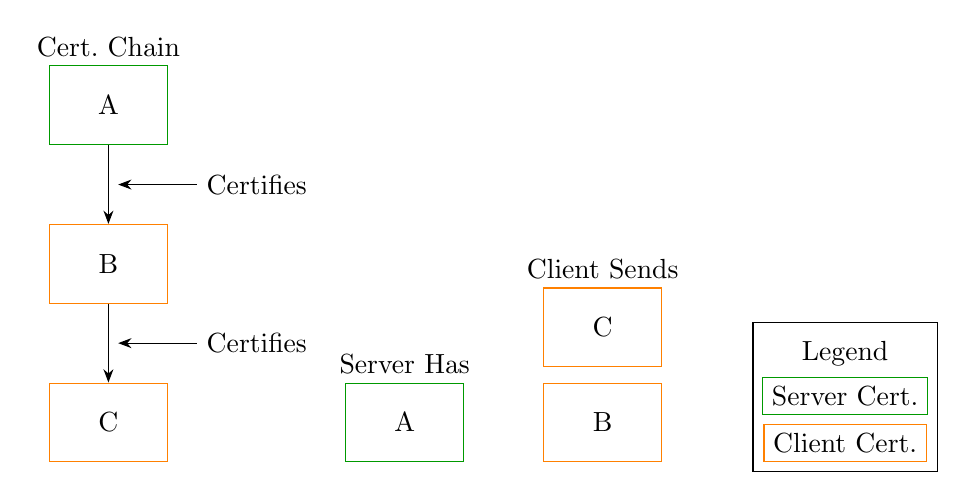
\begin{tikzpicture}
	% Styles.
	[s-cert/.style={rectangle,draw=green!60!black,minimum height=1cm,minimum width=1.5cm},
	c-cert/.style={rectangle,draw=orange,minimum height=1cm, minimum width=1.5cm}]
	% Certificate chain.
	\node (A) at (0, 0) [s-cert] {A};
	\node (B) [below=of A] [c-cert] {B};
	\node (C) [below=of B] [c-cert] {C};
	\draw[-Stealth] (A) -- (B)
		node[pos=0.5](a-cfies){};
	\node (a-cfies-txt) [right=of a-cfies] {Certifies};
	\draw[-Stealth] (a-cfies-txt) -- (a-cfies);
	\draw[-Stealth] (B) -- (C)
		node[pos=0.5](b-cfies){};
	\node (b-cfies-txt) [right=of b-cfies] {Certifies};
	\draw[-Stealth] (b-cfies-txt) -- (b-cfies);
	\node (txt) at (A) [above=0.5cm] {Cert.\ Chain};
	% Server certificates.
	\node (S-tmp) [right=of C] {};
	\node (S-A) [right=of S-tmp,s-cert] {A};
	\node (S-txt) at (S-A) [above=0.5cm] {Server Has};
	% Client certificates.
	\node (C-B) [right=of S-A,c-cert] {B};
	\node (C-C) at (C-B) [above=0.7cm,c-cert] {C};
	\node (C-txt) at (C-C) [above=0.5cm] {Client Sends};
	% Legend.
	\node (lanchor) at ($(current bounding box.south east) + (2, 0)$) {};
	\node (legend) at (lanchor) [above=1.1cm] {Legend};
	\node (l1) at (lanchor) [above=0.6cm,draw=green!60!black] {Server Cert.};
	\node (l2) at (lanchor) [above=0.0cm,draw=orange] {Client Cert.};
	\node [rectangle,draw,fit=(legend) (l1) (l2)] {};
\end{tikzpicture}
}
\end{makeimage}
\caption{Certificate chain where \texttt{A} is a trusted CA of the server and the client must send its certificate \texttt{C} followed by the intermediate certificate \texttt{B}.}
\end{figure}
\end{center}
After implementing a check for the entire peer certificate chain, my next problem was testing verification of the chain.  Consider the chain A -> B -> C, where A is trusted by the server and B and C are sent by the client.  I had been using OpenSSL's \texttt{s_client} command for testing, so the obvious approach was to place B and C into the file passed via the \texttt{-cert} argument; the first problem with this approach was that the certificates must be in a certain \emph{order}, specifically, the sender's certificate must come \emph{first}, followed by the certificate certifying the sender's certificate, and so on (see \htmladdnormallink{the RFC}{https://tools.ietf.org/html/rfc5246#section-7.4.2}).  In this case that meant sending C followed by B; specifying the certificates in the wrong order (B followed by C) was obvious, because \texttt{s_client} tried to use C's private key to verify B, which, of course, failed.  Putting them in the correct order, however, sent C while silently ignoring B.  After much gnashing of teeth, I decided to look into the source code, and, while combing through the parsing of the \texttt{-cert} option noticed an \emph{undocumented} (yes, not even in the \texttt{man} pages nor \texttt{-help} output) \texttt{-cert_chain} option.  After looking into it I ran the \texttt{s_client} command again with C sent via the \texttt{-cert} option and B sent via the \texttt{-cert_chain} option and was able to actually send a certificate chain to the server, and sanity was once again restored to my life.

\subsubsection{Testing}
Manually verifying changes is both a pain and error-prone, so I created a \htmladdnormallink{bash script}{https://github.com/clinew/inspircdtests/blob/master/ssl_strongcert.sh} in order to automatically test strong cert verification for InspIRCd on my system.  The tests check that the program runs without strong verification enabled, then turns verification on and checks that users can connect when their certificates use proper key type+sizes and algorithms, then checks that errors occur when invalid configuration options (such as non-existent algorithms) are specified, then finally checks that verification works correctly when the client passes a \emph{chain} of certificates.  It's not particularly exciting, but it gives peace of mind when rebasing on top of the latest stable release and when porting to newer versions of both OpenSSL and InspIRCd.

\subsection{Future Work}
After adding this feature I managed to find a series of functions that appeared as if they might do my heavy lifting for me.  The functions, found under the include directory as \texttt{ssl/ssl.h} were \texttt{SSL_set1_sigalgs_list()}, \texttt{SSL_set1_client_sigalgs_list()}, and a few similar variations.  Sadly, testing these show that they do not actually have the same functionality, although the signature algorithm list displayed after connecting via \texttt{s_client} was indeed different; presumably the signature algorithm is for session negation rather than peer certificate verification, but I am not yet sure as I have not yet Read The "Friendly" \strikeout{Manual} RFC.

The online man pages for the function also mentioned an \texttt{SSL_CONF} API, which might make option parsing easier; regardless, I didn't use it this time.


% Better Browsing With Firefox
\section{2018-01-17 Better Browsing With Firefox}
The Web is not what it once was, or at least not how I remember it.  It used to be like browsing a catalogue, with each link analogous to turning to a new page.  But the Web has transformed into something else entirely.  It is more like a \htmladdnormallink{two-way black mirror}{https://freedom-to-tinker.com/2017/11/15/no-boundaries-exfiltration-of-personal-data-by-session-replay-scripts} than a catalogue.  Every keystroke and mouse movement is logged and analyzed.  Users are tracked across unrelated websites by both visible widgets, invisible cookies, and more \htmladdnormallink{nefarious means}{https://en.wikipedia.org/wiki/Web_beacon}.  So-called "social media" sites analyze this data and censor their feeds in order to feed both themselves and their sponsors as much money as possible.  Basically, the Web has become a platform that consumes the user, rather than the user consuming the content of the Web.

Fortunately, there are ways to avoid being consumed by the Web and to create a more pleasant, catalogue-like browsing experience, but they are by no means obvious to the average person.  This blog will attempt to introduce the reader to some intermediate browsing techniques.  It assumes that the reader is already familiar with basic browser usage, and will then point out how, by installing a few add-ons, making a few configuration changes, and learning a few keystrokes, one's browsing experience can become both more controlled and more pleasant.  This requires work on the reader's part; it's not a give-me like most consumers desire, but tough shit, it's the world we currently live in.  This guide is divided into three sections, called "\htmladdnormallink{Power Levels}{https://www.youtube.com/watch?v=SiMHTK15Pik}", of increasing difficulty, with the first section requiring little to no work and having relatively little negative effect on one's browsing experience and a large positive effect, while the later sections require more work for often smaller gains.  Readers who are unsure of their skills should take a week or two in-between sections in order to familiarize themselves with any changes that they have made.

The Web browser of choice for this blog will be Firefox, because Firefox is \htmladdnormallink{Free Software}{https://www.gnu.org/philosophy/free-sw.en.html}.  Other common browsers, such as, but not limited to, Google Chrome, Safari, Microsoft Explorer, and Microsoft Edge are proprietary software and, therefore, \htmladdnormallink{considered harmful}{https://www.gnu.org/proprietary/proprietary.en.html}.  Make no mistake, Firefox has its flaws and its parent company, Mozilla Corporation, has made some \htmladdnormallink{questionable decisions}{http://lunduke.com/2017/12/17/mozilla-is-not-trustworthy}, but it's currently the best of the Free and featureful browsers to use.

\subsection{Power Level One}
\begin{figure}
\includegraphics[scale=0.5]{files/blog/2018_01_17_better_browsing_with_firefox/2018_01_17_ublockorigin_icon.png}
\caption{The uBlock Origin icon.}
\end{figure}
The first thing to do is to install the "uBlock Origin" add-on from the \htmladdnormallink{Mozilla Add-Ons}{https://addons.mozilla.org/en-US/firefox} webpage in order to block advertisements.  That's it.  Once it's installed, most advertisements will cease to be, and browsers without an ad-blocker will seem like a headache, because they are.  Sadly, a few sites will detect that one is using an ad-blocker and refuse to display any content, in which case you can disable the add-on \textit{for that site alone} by clicking on the uBlock Origin icon, then clicking the big ol' power-button icon in the drop-down menu that appears, but do note that most sites that are this ad-infested tend to suck and aren't worth reading anyways, in the same way that the trashiest magazines at the grocery checkout always have more advertisements than content in them.  Go figure.  Another icon worth noting is the little, Harry Potter-esque lightning icon, called the \textit{element zapper}.  Clicking on that icon will allow one to enter an element-zapper mode where one can select an element on the site for removal from their browser by clicking on it.  Hold \texttt{Shift} while clicking in order to continue removing elements, and press \texttt{Esc} to return to normal browsing mode.  Removals are not permanent, thus refreshing the page will reload any removed elements.  uBlock Origin can do this in part because it's actually a \textit{generic blocker} and not just an ad-blocker, but for now simply know that it's configured to block ads.

It's worth noting that there are other ad-blockers.  "AdBlock Plus" (ABP) is noteworthy for having been the de facto standard for a while before falling out of favor by many due to an \htmladdnormallink{"acceptable ads"}{https://adblockplus.org/acceptable-ads} campaign, in which certain, "unobtrusive" advertisements are not blocked by default and a portion of the revenue generated by the advertisements in sent to the ABP developers.  The AdBlock Plus add-on also tends to take up far more memory than uBlock Origin, which gave me issues on my low-memory machines, thus I prefer uBlock Origin for that reason alone.  There's also "uBlock", which was originally developed by the author of uBlock Origin, but apparently there were some issues and now the original author is working on uBlock Origin and that's what I've decided to use.  Feel free to check out the other one if you are so inclined.

\begin{figure}
\includegraphics[scale=0.5]{files/blog/2018_01_17_better_browsing_with_firefox/2018_01_17_httpseverywhere_icon.png}
\caption{The HTTPS Everywhere icon.}
\end{figure}
The next thing to do is to install the "HTTPS Everywhere" add-on developed by the \htmladdnormallink{Electronic Frontier Foundation}{https://www.eff.org/} (EFF).  A brief explanation is in order: HyperText Transfer Protocol (HTTP) is the protocol used for the Web, and HTTP\textbf{S} is, roughly speaking, the \textit{\textbf{S}ecure} version of that protocol.  HTTPS is useful because it's the reason \htmladdnormallink{crackers}{https://stallman.org/articles/on-hacking.html} cannot easily break into your bank account or use your credit card when you are browsing the web.  Many sites offer both secured and unsecured versions of their webpages but configure their websites such that users must explicitly request the secure version of the website by prefixing the address with \texttt{https://}, which is a giant pain in the ass.  HTTPS Everywhere fixes this problem by automatically \textit{rewriting} (a.k.a. "changing") any HTTP addresses to their secure, HTTPS variants, no user intervention required.  This is done through a database of sites that comes with the program; the database knows how to rewrite addresses for different sites.  Although a few, very obscure sites may not have their addresses rewritten, the vast majority will.

Lastly, it is worth learning one mouse click technique and a few simple key-commands.  Most mice have a scroll wheel in the middle, and that scroll wheel can be pressed in order to generate a "middle-mouse button click", or "middle-click" for short.  Middle-clicking a link will open said link in a new tab.  This is far faster than going through the tedious process of right-clicking the link and then selecting "Open in New Tab" from the drop-down menu.  It's a serious time-saver.  Use it.  The middle-mouse click can also be used to close a tab by clicking on the tab itself.  Ever accidentally close a tab and then realized that it shouldn't have been closed?  Type \texttt{Ctrl-Shift-T} to bring it back!  Continue typing the command in order to bring back tabs in the order in which they were closed.  Finally, \texttt{Ctrl-F} can be used to \textit{Find} text within a webpage.  Just in case one wasn't aware.

That's it for this first section.  One's browsing experience should now be ad-free, far more secure, and hopefully a little bit smoother with those middle-clicks.  There probably won't be any disruption in one's browsing experience, but take some time to get used to it before proceeding onto the next section.

\subsection{Power Level Two}
This section will impact one's browsing experience far more than the previous section.  This section also plays the largest part in disabling the two-way mirror "functionality" of the Web.  This involves changing a few configuration options, installing a new add-on, and finally learning a few keyboard shortcuts.

Begin by making some configuration changes to Firefox that will cause each \textit{session} to be independent of the others.  In other words, each time Firefox is closed and opened it will be as if no websites had been visited during the previous time Firefox was open, even if they were, as if Firefox had just been installed, except, of course, the add-ons, bookmarks, and other user-defined settings will remain.  I could try and describe the bloody icons that lead to the \texttt{Preferences} menu, but it'll be easier if I tell you to simply type \texttt{F10} to open the old-style text-based menu and then navigate to \texttt{Edit -> Preferences}.  From there, click on the tab labeled \texttt{Privacy}, then find the section labelled \texttt{History} and change the corresponding drop-down to \texttt{Never remember history}.  Likewise, next find the section labelled \texttt{Location Bar} and uncheck all of the boxes.  Lastly, click on the tab labelled \texttt{Advanced}, then another tab labelled \texttt{Network} and finally the section labelled \texttt{Cached Web Content} and check the \texttt{Override automatic cache management} checkbox and then set the specified value to \texttt{0 MB}.  That should make each browsing session far more independent and thus make tracking more difficult, but it will be noticeable as many sites that require a login will no longer "remember" one's username and one will thus have to type it in again.

\begin{figure}
\includegraphics[scale=0.5]{files/blog/2018_01_17_better_browsing_with_firefox/2018_01_17_noscript_icon.png}
\caption{The NoScript icon.}
\end{figure}
Next comes the biggest change: installing the "NoScript" add-on.  This add-on is what allows one to selectively enable and disable JavaScript.  Unlike plain HTML, JavaScript is actually code that is sent by the web server and run on the user's computer.  This code is what allows the browser to track the user's mouse movements, keystrokes, and gather various information about the user's system.  The fact that browsers run arbitrary JavaScript code on the user's computer is a large part of what turns the Web from a catalogue into a two-way mirror (confusingly enough, JavaScript has no relationship to the Java programming language).  What NoScript does is to give one some control over what JavaScript is run on their computer.  The default is to block all JavaScript, which will cause many sites to break, but scripts can be allowed on a per-site basis by clicking the NoScript icon and then selecting \texttt{Temporarily allow from <address>} from the drop-down menu where \texttt{<address>} is the name of the site that the JavaScript is loaded from, and when the drop-down menu is closed the site will automatically reload with the selected scripts enabled.  Note that most sites load JavaScript from multiple sources, thus the \texttt{Temporarily allow all this page} option can come in handy when one wants to load all scripts on the site, but note, however, that some scripts will then drag in other scripts, and thus for certain sites one will have to "allow all" for the site multiple times.  Note that any allowances made will apply to \textit{all} tabs that one has opened, not just the current tab.  When one no longer wishes to allow scripts, clicking the icon again and selecting the \texttt{Revoke temporary permissions} will disable all scripts and refresh the sites whose scripts were revoked.  It's actually quite simple once one gets the hang of it.

After using NoScript for a while one will inevitably notice that certain addresses come up again and again.  Most notorious in my opinion is \texttt{google-analytics.com}.  Since I have absolutely no desire to be analyzed by The Googlaug ever, I banished the script permanently by clicking the NoScript icon, then selecting \texttt{Untrusted -> Mark google-analytics.com as untrusted}, thus removing it from the drop-down menu.  Good riddance.  The drop-down menu can be customized by selecting \texttt{Options} and then the \texttt{Appearance} tab and toggling the various boxes.  It can be useful to uncheck the \texttt{Allow [...]} and \texttt{Allow all this page} boxes if one does not wish to even accidentally give some scripts permanent permission.

Now, NoScript actually does a little more than just block JavaScript, it also protects against a few types of Web-based attacks by blocking \htmladdnormallink{Cross-Site Scripting (XSS)}{https://en.wikipedia.org/wiki/Cross-site_scripting} and implementing \htmladdnormallink{Application Boundary Enforcer (ABE)}{https://noscript.net/abe/}.  Although these are generally considered a Good Thing (TM), they occasionally cause problems with crappy Web portals, for example, at one's local library where one is required to agree to a Terms of Service (ToS), and need to be disabled.  ABE can usually be worked around by choosing the "Unsafe Reload" option after it has been triggered, but both can be disabled by opening the options window, selecting the \texttt{Advanced} tab and then selecting either the \texttt{XSS} or \texttt{ABE} tab and turning the offending feature off.  With that one should now have some basic control over the JavaScript run on one's own computer.

A few more useful key-commands are now in order.  First, \texttt{Ctrl-L} and \texttt{Ctrl-J} move the cursor to the Location and Search Bar, respectively.  For tab-management, \texttt{Ctrl-T} opens a new tab, \texttt{Ctrl-W} closes the current tab, and \texttt{Ctrl-Q} quits the browser program; because the \texttt{Q} key is right next to the \texttt{W} key, it's a good idea to keep the "Warn me when I attempt to close multiple tabs" checkbox enabled.  Lastly, use \texttt{Ctrl-PgUp} (Page Up) and \texttt{Ctrl-PgDn} (Page Down) in order to move to the previous and subsequent tab, respectively.

Thus ends the second section.  Each browser session should now be more independent and two-way mirror functionality will be disabled by default.  These are both rather large changes to make, but they offer significant privacy and security advantages, so the added difficulty is often worthwhile.  Make sure to become comfortable with these changes before moving onto the next section.

\subsection{Power Level Three}
As explained in the first section, uBlock Origin is actually a \textit{generic blocker}, meaning that it can block more than just ads.  Ad-blocking is actually done via a \textit{filter list} which is provided by a third party, and there exist more than just ad-filter lists, for example, filter lists to block embedded tracking widgets from sites like Farcebook.  In order to view the filter lists, click on the uBlock Origin icon and then click on the icon that looks like, uh, well, three lines with some kind of slider-thingies on it (damn icons) in order to open the "dashboard", and then click on the "3rd party filters" tab in order to view a default list of filters.  Learn more about each filter by clicking on the house icon in order to be directed to a webpage containing information about the filter, and enable/disable filters by checking/unchecking their respective boxes.  I like "Fanboy's Social Blocking List" myself.  One can also manually update their lists by clicking the obvious "Update Now" button while on this tab.

Filter lists are nice for most uses, but sometimes one needs custom filters on a site; this can be done by clicking "I am an advanced user" in the dashboard's "Settings" tab and thus enabling \textit{dynamic filtering}; make sure to read the corresponding documentation under \htmladdnormallink{required reading}{https://github.com/gorhill/uBlock/wiki/Advanced-user-features} before trying to apply any dynamic filters; they are not covered here because the existing documentation is better than what I would write.  Note that after enabling dynamic filtering it's interesting enough to simply click on the uBlock Origin icon after loading a site and seeing which sites one's browser has connected to.  In a similar vein to the zapper icon (in the menu that appears after clicking the uBlock Origin icon), the eye-dropper, or \textit{element picker}, helps create custom filter rules rather than simply removing an element until the page is reloaded, but be careful about the filters it creates unless one wants to filter more than intended.  Adding custom filters in more of an art than a science, but it provides incredible control over which services get to track one's virtual movement across the Web.

When customizing Firefox, one might be tempted to naively believe that, after clicking on the gear icon and perusing all sections and tabs and setting things up as one desires that they're finished with all possible non-add-on-based customizations.  However, Firefox, in fact, actually has a, well, it's not exactly \textbf{hidden}, but \textbf{unadvertised}, perhaps, customization menu that can be reached by typing \texttt{about:config} into the address bar (then hitting \texttt{Enter}, obviously).  This page consists of a list of \textit{preferences} with a \textit{type} and \textit{value} and whose values can be customized by the user.  A full discussion of all preferences in this menu would likely require an entire encyclopedia, so only a few noteworthy preferences are mentioned here.  First off is the \texttt{UserAgent}, which is a string containing various client metadata such as operating system, browser vendor, browser version, \&c, and which is sent to the web server when the connection is first established so that the web server can serve up client-specific \htmladdnormallink{hacks}{https://en.wikipedia.org/wiki/Hack_(computer_science)}, \htmladdnormallink{nevermind that the whole damn point of the web was to be platform-independent}{http://www.catb.org/~esr/html-hell.html}.  One can view their \texttt{UserAgent} by navigating to \texttt{about:} in the address bar, and one can customize it in the \texttt{about:config} menu by right-clicking then selecting \texttt{New -> String} and then giving the preference name \texttt{general.useragent.override} and then providing whatever value one wants; check \texttt{about:config} to confirm.  Note that poorly-designed sites will break if they can't supply custom browser-specific hacks, for example, this is what Googlaug Voice looks like with the classy \texttt{UserAgent} of "Fuck JavaScript":
\begin{figure}
\includegraphics[scale=0.33]{files/blog/2018_01_17_better_browsing_with_firefox/2018_01_17_googlaug_voice.png}
\caption{These modern interfaces really know how to cut down on bloat!}
\end{figure}
Note that using a custom \texttt{UserAgent} is \htmladdnormallink{probably less anonymous than one might think}{https://panopticlick.eff.org/}.

A few other noteworthy preferences are \texttt{javascript.options.asmjs} which allows JavaScript to run native code on one's computer and will probably cause some security nightmare within the next decade or two (set it to \texttt{false} now).  One may also wish to set \texttt{webgl.disabled} to \texttt{true}, although NoScript already forbids WebGL by default.  Due to \htmladdnormallink{recent events}{https://sircmpwn.github.io/2017/12/16/Firefox-is-on-a-slippery-slope.html} one will probably want to set \texttt{experiments.enabled} to \texttt{false}.  Note that while one might be tempted to set \texttt{javascript.enabled} to \texttt{false}, JavaScript is actually used internally by the browser and add-ons, and thus disabling it here actually causes add-ons to not function properly, relying on NoScript is recommended instead.

This section has been rather open-ended, because customizations at this point have become, well, highly-customized.  Nonetheless, one should now have an idea of how to go about blocking content on websites they visit and performing deep configuration of Firefox.

\subsection{Conclusion}
That's it for this guide.  Hopefully one's browser experience is now both cleaner and more controlled than it had been before.  While it may have been a large amount of information to take in, please understand that there is still much more to be learned about the Web and its oftentimes questionable behaviour, and please note that none of these techniques are meant to make one anonymous, as that is the aim of other projects such as \htmladdnormallink{Tor}{https://torproject.org} and \htmladdnormallink{TAILS}{https://tails.boum.org}.  Regardless, one who has followed this guide should now be able to begin taking back control of their Web experience.  Good luck.


% 4.9-4.14 Kernel Upgrade USB Woes
\section{2018-01-08 4.9-4.14 Kernel Upgrade USB Woes}
Given the recent concerns over the Meltdown/Spectre vulnerabilities and the release of \htmladdnormallink{new stable kernels}{https://lwn.net/Articles/743246/}, I figured that now would be a good time to do a quick kernel upgrade.  As you have probably surmised by the very existence of this blog post, the "quick" upgrade turned into a bit of a headache.

Rather than using another 4.9 kernel with a backported mitigation, I decided that now would be a good time to upgrade to the newer 4.14 kernel.  The usual process went smoothly: downloading, verifying the signature, updating the configuration, compiling, and finally booting.  Except there was one little problem after booting: I couldn't enter my passphrase from my keyboard in order to decrypt the root filesystem.  Huh?  The keyboard, which is a USB keyboard, had worked before the BIOS hand-off, and it still had power, but no key-presses, even SysRq keys, had any effect.  Other than that, the kernel seemed perfectly fine, no backtraces or nasty error messages being spewed out.

Okay, well, at this point I was rather dumbfounded.  Nothing in the output of \texttt{make oldconfig} that I could recall suggested something that would break my USB keyboard, and the only thing that I really cared about in this upgrade was the new Kernel Page-Table Isolation (KPTI) feature, but maybe this was some weird bug with it and my \texttt{initramfs}, so I tried disabling it, recompiling the kernel, and booting the recompiled kernel.  Still broken.  So, at least the security feature that I'd upgraded for wasn't the source of my woes, but that didn't solve my problem.  At this point it also occurred to me that no messages for the attached USB storage device were showing up, either, so this was some kind of USB problem.  Perhaps the problem was specific to the front ports?  I decided to try the back ports, which are attached directly to the motherboard, and did not have any luck there, either.

Perhaps I'd missed something when updating the configuration, so I saved my new configuration and re-ran \texttt{make oldconfig} on a copy of the old configuration and noted any options that \textit{might possibly} be affecting my USB devices.  A few possibilities emerged, including \texttt{X86_MCELOG_LEGACY} (the \texttt{initramfs} is rather old), \texttt{SERIAL_DEV_BUS} (are the USB devices connected to the motherboard via serial?), \texttt{RC_CORE} (uhh do I have video capture?), \texttt{USB_PCI}, and \texttt{USB_HUB_USB251XB}.  The latter two options seemed the most suspicious.  The help information for \texttt{USB_PCI} reads:
\begin{quote}
\begin{verbatim}
	A lot of embeded system SOC (e.g. freescale T2080) have both
	PCI and USB modules. But USB module is controlled by registers
	directly, it have no relationship with PCI module.

	When say N here it will not build PCI related code in USB driver.
\end{verbatim}
\end{quote}
English is obviously not their native language, but code isn't mine, so fair's fair.  It sounds like there's PCI code in the USB module for\ldots~no reason?  Well, I don't have any USB hubs connected via PCI add-on cards, so this should be safe left disabled.  Regarding \texttt{USB_HUB_USB251XB}, perhaps some hub-specific code got moved into a separate option and I happen to be using that hub.

No clear winner emerged, so I opened the case in order to examine how the USB ports were connected and what hubs were in use:
\begin{figure}
\includegraphics[scale=0.5]{files/blog/2018_01_08_kernel_upgrade_usb_woes/motherboard.png}
\caption{"Can you find the PCI USB on this motherboard?  Neither could we."}
\end{figure}
The back ports are directly connected to the motherboard, and the front ports are connected by some\ldots~thing to the motherboard.  I have no idea how components on the motherboard are interconnected (I2C?, serial?, gnomes?), but the USB hubs are certainly not connected via PCI cards, and I couldn't find any "USB251XB" markings on or around the hubs, not that I could particularly make out the small, cryptic writings on the board anyhow.  After blowing out some dust and a couple of sneezes later I went back to scratching my head.  Perhaps \texttt{make oldconfig} didn't tell me everything.  I decided to run a \texttt{diff -u} in-between the old and new configuration, and one line in particular caught my eye:
\begin{quote}
\begin{verbatim}
	-CONFIG_USB_UHCI_HCD=y
\end{verbatim}
\end{quote}
Now I cannot for the life of me remember what each of the \texttt{_HCI} USB configurations refer to what vendor/version combination, but this seemed like a \textit{very} strange omission.  Going into \texttt{menuconfig} and searching for the option was even more telling:
\begin{quote}
\begin{verbatim}
	Prompt: UHCI HCD (most Intel and VIA) support
\end{verbatim}
\end{quote}
"most Intel", eh?  So why was this option magically unselected?
\begin{quote}
\begin{verbatim}
	Depends on: USB_SUPPORT [=y] && USB [=y] && (USB_PCI [=n] || USB_UHCI_SUPPORT_NON_PCI_HC [=n])
\end{verbatim}
\end{quote}
Right, so, disabling the new \texttt{USB_PCI} option will \textit{silently} disable \texttt{USB_UHCI_HCD} \textit{even if it was already selected}.  Could this be my problem?  I enabled both \texttt{USB_PCI} and \texttt{USB_UHCI_HCD}, recompiled, booted, and, lo and behold, my USB devices started working again.

So much for a "quick" upgrade.  While I'm glad to have things working again, it would have been nice if the \texttt{USB_PCI} help had clarified that whether or not PCI code is needed in the USB module \textit{depends on the system}, because the current wording suggests that it \textit{never} has any relationship to the PCI module ("it have no relationship with PCI module", said without qualifications).  Something along the lines of, "in these embedded systems, the USB module has no relationship to the PCI module" would have been better.  It also would have been nice if the \texttt{USB_UHCI_HCD} options wasn't silently disabled, but that may be a limitation of the Kconfig language; I don't know.  At least things are working again\ldots~at least until the other cache vulnerabilities start being exploited \texttt{;)}.


% Booting BeagleBone Black With an Initramfs
\section{2017-10-05 Booting BeagleBone Black With an Initramfs}
\begin{center}
\begin{figure}
\begin{makeimage}
\newcommand{\fn}[1]{\hspace*{1ex}\texttt{#1}}
\fbox{
\begin{tabular}{l l}
Before: & After: \\
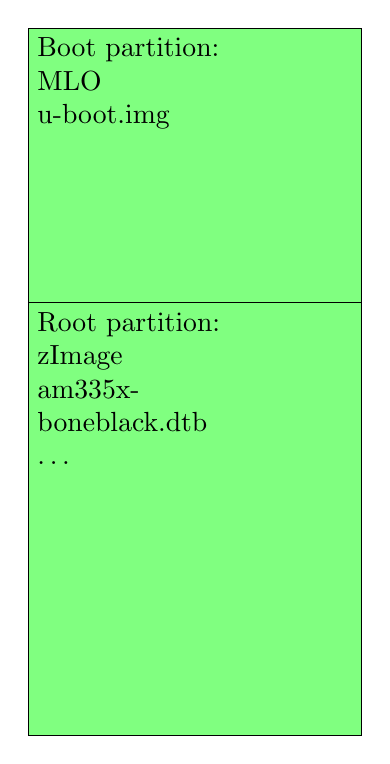
\begin{tikzpicture}
	\node at (0, 0) [rectangle split,rectangle split parts=2,rectangle split part fill={green!50, green!50},align=left,draw,text width=4cm]
		{\rule[-3cm]{0cm}{3cm}\parbox[t]{3cm}{Boot partition: \\ \fn{MLO} \\ \fn{u-boot.img}}
		\nodepart{two} \rule[-5cm]{0cm}{5cm}\parbox[t]{3cm}{Root partition: \\ \fn{zImage} \\ \fn{am335x-boneblack.dtb} \\ \fn{\ldots}}};
\end{tikzpicture}
&
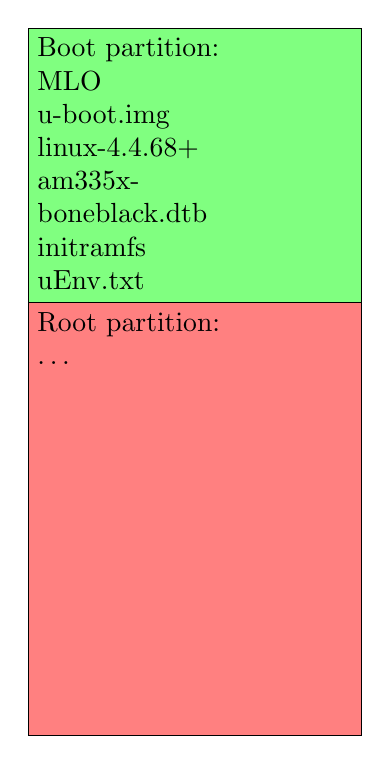
\begin{tikzpicture}
	\node at (0, 0) [rectangle split,rectangle split parts=2,rectangle split part fill={green!50, red!50},align=left,draw,text width=4cm]
		{\rule[-3cm]{0cm}{3cm}\parbox[t]{3cm}{Boot partition: \\ \fn{MLO} \\ \fn{u-boot.img} \\ \fn{linux-4.4.68+} \\ \fn{am335x-boneblack.dtb} \\ \fn{initramfs} \\ \fn{uEnv.txt}}
		\nodepart{two} \rule[-5cm]{0cm}{5cm}\parbox[t]{3cm}{Root partition: \\ \fn{\ldots}}};
\end{tikzpicture}
\end{tabular}
\begin{tabular}{c l}
\multicolumn{2}{c}{\textbf{Legend}} \\

\begin{tikzpicture}
	\node at (0, 0) [fill=green!50,draw] {};
\end{tikzpicture} & Unencrypted \\

\begin{tikzpicture}
	\node at (0, 0) [fill=red!50,draw] {};
\end{tikzpicture} & Encrypted
\end{tabular}
}
\end{makeimage}
\caption{Visualization of the SD Card before and after modifications.  Contents are not to scale.}
\end{figure}
\end{center}

The instructions for installing Gentoo on my BeagleBone Black (BBB)\htmladdnormallink{[1]}{https://wiki.gentoo.org/wiki/BeagleBone_Black} gave me a working OS, but one without the root partition encrypted.  Unencrypted OSes make me sad, but an encrypted root partition means using an \texttt{initramfs}; to make matters more complicated, the kernel and device tree are on the root partition, but they need to be on the boot partition (because the root partition will be encrypted).  This blog will explain how I was able to make these changes; it will not cover creating an \texttt{initramfs} nor creating an encrypted root partition using LUKS and \texttt{cryptsetup}.

\subsection{Das U-Boot}
Das U-Boot, colloquially known simply as "U-Boot", is roughly analogous to the BIOS and/or UEFI portion of normal desktop towers.  Like desktops, the boot process can be interrupted and the user taken to a configuration interface by typing a certain key early on in the boot process.  For the BBB, this can be done by pressing the 'Space' button, which takes the user to a Command-Line Interface (CLI); from here, \texttt{help} may be run in order to provide a list of commands or to print usage information for a specific command.  One of the most useful commands to run is \texttt{printenv}, which will list all of the environment variables; these variable are important because their values can be either simple values or an entire script.  It is these variables that must be modified in order to load and boot an \texttt{initramfs}, kernel, and device tree file from the boot partition.

While one can modify the environment variables before each boot, this is extremely tedious.  Thankfully, U-Boot allows one to define a \texttt{uEnv.txt} file in the boot partition that will be read in before the boot process is completed and which will set the environment variables as specified in the file.  Thus one can simply write this file rather than constantly modify the environment variables at each boot.

\subsection{uEnv.txt}
This section will explain what variables I added/modified and why I modified them.  Though they are all crammed together in the actual file, for conceptual purposes I will divide them into three categories: filename definitions, load scripts, and boot scripts.

The first of the sections, filename definitions, is straightforward enough:
\begin{quote}
\begin{verbatim}
	# BEFORE
	bootfile=zImage
	# AFTER
	bootfile=linux-4.4.68+
	rdfile=initramfs
\end{verbatim}
\end{quote}
Although changing the name from \texttt{zImage} to \texttt{linux-4.4.68+} isn't strictly necessary, I prefer to have my kernels include their version in the name as it makes booting, upgrading, and dealing with regressions easier.  The \texttt{rdfile} variable is added for consistency with the existence of the \texttt{bootfile} variable, and is used later.  Note that the same \texttt{initramfs} can often be used across multiple kernel versions.

The second section, load scripts, consists of the series of commands used to load the kernel, initramfs, and device tree into memory:
\begin{quote}
\begin{verbatim}
	# BEFORE
	loadimage=load ${devtype} ${bootpart} ${loadaddr} ${bootdir}/${bootfile}
	loadfdt=load ${devtype} ${bootpart} ${fdtaddr} ${bootdir}/${fdtfile}
	loadramdisk=load mmc ${mmcdev} ${rdaddr} ramdisk.gz
	# AFTER
	loadimage=fatload mmc ${mmcdev} ${loadaddr} ${bootfile}
	loadfdt=fatload mmc ${mmcdev} ${fdtaddr} ${fdtfile}
	loadramdisk=fatload mmc ${mmcdev} ${rdaddr} ${rdfile}
\end{verbatim}
\end{quote}
A few things are worth noting here.  First is that I ignored the \texttt{devtype} and \texttt{bootpart} variables and just loaded the kernel (\texttt{loadimage}), device tree (\texttt{loadfdt}), and initramfs (\texttt{loadramdisk}) directly from the MMC (SD Card), since that is what I wanted; this worked on my SD Card, but may be fragile on other configurations, use at your own risk!  Second, there is already an instruction for loading a ramdisk which, from a cursory glance of other environment variables, appears to be associated with boot code for a live OS rather than an \texttt{initramfs} for booting; since I currently am not interested in nor know how to use this functionality, it appears safe to modify.  Last, I removed the \texttt{bootdir} prefix for the kernel and device tree filepaths, since I'm simply going to place them at the root directory of the boot partition.

The last section, boot scripts, is the most complicated section, because it contains the commands and logic needed to actually boot the system:
\begin{quote}
\begin{verbatim}
	# BEFORE
	args_mmc=run finduuid;setenv bootargs console=${console} ${optargs} root=PARTUUID=${uuid} rw rootfstype=${mmcrootfstype}
	mmcloados=run args_mmc; if test ${boot_fdt} = yes || test ${boot_fdt} = try; then if run loadfdt; then bootz ${loadaddr} - ${fdtaddr}; else if test ${boot_fdt} = try; then bootz; else echo WARN: Cannot load the DT; fi; fi; else bootz; fi;
	# AFTER
	args_mmc=run finduuid;setenv bootargs console=${console} ${optargs} root=/dev/mapper/mmcblk0p2 initrd=initramfs rw rootfstype=${mmcrootfstype}
	mmcloados=run args_mmc; run loadramdisk; if test ${boot_fdt} = yes || test ${boot_fdt} = try; then if run loadfdt; then bootz ${loadaddr} ${rdaddr} ${fdtaddr}; else if test ${boot_fdt} = try; then bootz; else echo WARN: Cannot load the DT; fi; fi; else bootz; fi;
\end{verbatim}
\end{quote}
While the commands may appear relatively complex, the modifications are actually pretty simple.  For \texttt{args_mmc}, the \texttt{root=PARTUUID=\${uuid}} had to be changed to the mapping set up by the encryption scripts, in my case to \texttt{root=/dev/mapper/mmcblk0p2}; the argument \texttt{initrd=initramfs} was also added to let the kernel know about the \texttt{initramfs} file (but may not strictly be necessary in this context).  Two modifications were made to \texttt{mmcloados}: the first was to load the initramfs by calling \texttt{run loadramdisk;}, the second was to change the \texttt{bootz} command to contain the address of the \texttt{initramfs} to load (\texttt{rdaddr}) rather than not loading one (\texttt{-}).

Thus with each of these modifications I was able to boot with an encrypted root partition.  Hopefully you will have the same luck, and don't forget to copy your files from the root partition to the boot partition!


% Adding Certificate Revocation Lists (CRLs) to an Existing OpenSSL Implementation.
\section{2017-09-22 Adding Certificate Revocation Lists (CRLs) to an Existing OpenSSL Implementation}
I recently took it upon myself to add Certificate Revocation List (CRL) functionality to an SSL-enabled program (\htmladdnormallink{InspIRCd}{https://github.com/inspircd/inspircd/pull/1370}).  This blog details both the code that I used and some unexpected functionality regarding how CRLs behave.  Hopefully this blog will prove useful to someone else who needs to tread this path.

\subsection{Code Itself}
The code itself is actually quite simple, consisting of two basic steps: loading the CRL files and then enabling CRL checking.  In order to load the CRL files, begin by getting the \texttt{X509_STORE *} from the \texttt{SSL_CTX *} by calling \texttt{SSL_CTX_get_cert_store(3)}, then load the CRL files into the \texttt{X509_STORE *} by calling \texttt{X509_STORE_load_locations()} with the specified CRL file and path locations.  The definition of the functions can be found in \texttt{openssl/x509_vfy.h} in your system's include file directory.  The code looks something like:
\begin{quote}
\begin{verbatim}
	SSL_CTX *ctx = sslctx; // Defined elsewhere.
	X509_STORE *store;
	char *crlfile = "/path/to/single/file.pem";
	char *crlpath = "/path/to/entire/directory";

	if (!(store = SSL_CTX_get_cert_store(ctx))) {
		fprintf(stderr, "No cert store found\n");
		return -1;
	}
	if (!X509_STORE_load_locations(store, crlfile, crlpath)) {
		fprintf(stderr, "Unable to load CRL files\n");
		return -1;
	}
\end{verbatim}
\end{quote}
This will load the CRL files, but will not enable CRL checking; this has to be done by setting a flag value in the \texttt{X509_STORE *}.  There at least two possible options: one is to check only the leaf certificate, the other is to check all certificates in the chain.  The former option can be accomplished by setting only \texttt{X509_V_FLAG_CRL_CHECK} while the latter can be accomplished by setting two flags \texttt{X509_V_FLAG_CRL_CHECK | X509_V_FLAG_CRL_CHECK_ALL}.  The latter option (the entire chain) is almost certainly what you want.
\begin{quote}
\begin{verbatim}
	char* crlmode; // Defined elsewhere.
	int crlflags;

	if (!strcmp(crlmode, "chain")) {
		crlflags = X509_V_FLAG_CRL_CHECK | X509_V_FLAG_CRL_CHECK_ALL;
	} else if (!strcmp(crlmode, "leaf")) {
		crlflags = X509_V_FLAG_CRL_CHECK;
	} else {
		fprintf(stderr, "Unknown flag mode '%s'\n", crlmode);
		return -1;
	}
	if (X509_STORE_set_flags(store, crlflags) != 1) {
		fprintf(stderr, "Unable to set flags\n");
		return -1;
	}
\end{verbatim}
\end{quote}
\ldots and that's it!  CRLs should now be enabled for your program.  However, do not rest easily just yet, as CRLs offer several pitfalls for the unwary, as detailed below.

\subsection{Missing CRL Files}
Consider\label{2017-09-22-missing-crls} the following, simple certificate chain:
\begin{center}
\begin{figure}
\begin{makeimage}
\fbox{
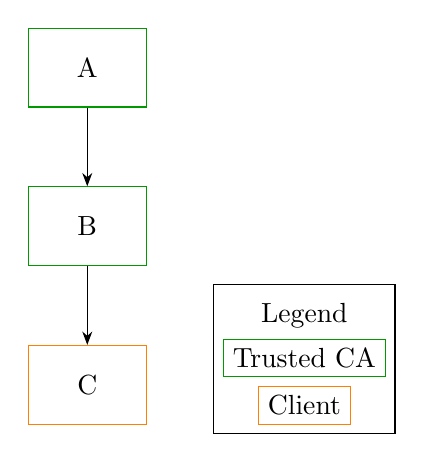
\begin{tikzpicture}
	% Styles.
	[ca/.style={rectangle,draw=green!60!black,minimum height=1cm,minimum width=1.5cm},
	leaf/.style={rectangle,draw=orange,minimum height=1cm, minimum width=1.5cm}]
	% Certificates.
	\node (A) at (0, 0) [ca] {A};
	\node (B) [below=of A] [ca] {B};
	\node (C) [below=of B] [leaf] {C};
	\draw[-Stealth] (A) -- (B);
	\draw[-Stealth] (B) -- (C);
	% Legend.
	\node (lanchor) at ($(current bounding box.south east) + (2, 0)$) {};
	\node (legend) at (lanchor) [above=1.1cm] {Legend};
	\node (l1) at (lanchor) [above=0.6cm,draw=green!60!black] {Trusted CA};
	\node (l2) at (lanchor) [above=0.0cm,draw=orange] {Client};
	\node [rectangle,draw,fit=(legend) (l1) (l2)] {};
\end{tikzpicture}
}
\end{makeimage}
\caption{Simple certificate chain, where A and B are CAs and C is the client.}
\end{figure}
\end{center}
The server trusts Certificate Authorities (CAs) A and B to issue valid certificates, thus C's certificate will be accepted.  Without CRLs this scenario will work as expected, C will be able to connect to the server without a problem.  Now, assume that the server enables CRLs, generates a CRL for A, and then configures itself to use A's CRL; a CRL for B is not generated as B has not revoked any certificate and thus there doesn't \emph{seem} to be any need to generate a CRL for B.  As you can probably guess by now, C will not be able to connect in this scenario, because the default CRL-checking method requires \emph{every} CA in the chain to have a CRL file loaded, thus C cannot connect unless both A \emph{and} B generate CRL files, \emph{even if they have no revoked certificates}.
\begin{center}
\begin{figure}
\begin{makeimage}
\fbox{
\begin{tikzpicture}
	% Styles.
	[ca/.style={rectangle,draw=green!60!black,minimum height=1cm,minimum width=1.5cm},
	leaf/.style={rectangle,draw=red,minimum height=1cm, minimum width=1.5cm},
	x/.pic={
		\draw[--] (-1mm,1mm) -- (1mm,-1mm);
		\draw[--] (-1mm,-1mm) -- (1mm,1mm);
	}]
	% Certificates.
	\node (A) at (0, 0) [ca] {A};
	\node (B) [below=of A] [ca] {B};
	\node (C) [below=of B] [leaf] {C};
	\draw[-Stealth] (A) -- (B);
	\draw[-Stealth] (B) -- (C)
		node[pos=0.5](fail){}
		pic [pos=0.5,red] {x};
	\node (error) [right=of fail] {No CRL file for B};
	\draw[-Stealth] (error) -- (fail);
	% Legend.
	\node (lanchor) at ($(current bounding box.south east) + (1.5, 0)$) {};
	\node (legend) at (lanchor) [above=1.1cm] {Legend};
	\node (l1) at (lanchor) [above=0.6cm,draw=green!60!black] {Trusted CA};
	\node (l2) at (lanchor) [above=0.0cm,draw=red] {Client};
	\node [rectangle,draw,fit=(legend) (l1) (l2)] {};
\end{tikzpicture}
}
\end{makeimage}
\caption{Each CA is required to have a CRL file.}
\end{figure}
\end{center}

The consequence of this is that enabling CRL-checking requires gathering CRL files, a task that is likely non-trivial.  The alternative is to override OpenSSL's verify callback by defining your own verify function and then telling OpenSSL to use said function with \texttt{X509_STORE_set_verify_cb(3)}.  I, however, do not intend to touch that with a 10-foot pole.

\subsection{Using a CRL Path}
Suppose that you wish to use a directory to store CRL files separately for each CA (instead of one big CRL file), then have OpenSSL load in each CRL file from this directory.  An obvious benefit of this approach is that it allows you to create a separate CRL file for each CA; using the certificate chain from the previous section, this would mean a directory containing both \texttt{crl/a.pem} and \texttt{crl/b.pem}.  One would think that it would be enough to place each CRL file in said directory, then point OpenSSL to said directory, but that actually doesn't work.

While OpenSSL indeed expects each CA to have its own CRL file, it expects the CA file to be named in a very specific manner; it expects the file to be named as the concatenation of the first part of the \emph{hash} of its issuer name and \texttt{.rX} where \texttt{X} starts as \texttt{0} and is incremented for each hash collision that occurs.  For example, suppose the hash of CA B is \texttt{deadbeef}, then its CRL filename is expected to be \texttt{deadbeef.r0}.  Arguably, the easiest way to support this hash-based filename is to create the actual CRL file with the name of its respective issuer, then create the symbolic link for OpenSSL, which can be done by something like:
\begin{quote}
\begin{verbatim}
	for crl in `ls *.pem`; do
		hash=$(openssl crl -hash -in "${crl}" -noout)
		# Just assume no collisions for simplicity.
		ln -s "${crl}" "${hash%$'\n'}.r0"
	done
\end{verbatim}
\end{quote}
\ldots which generates a hash for each file suffixed with \texttt{.pem} in the current directory (WARNING: does not take into account hash collisions).  With the symbolic links created, you should now be able to use a CRL path.

\begin{center}
\begin{figure}
\begin{makeimage}
\fbox{
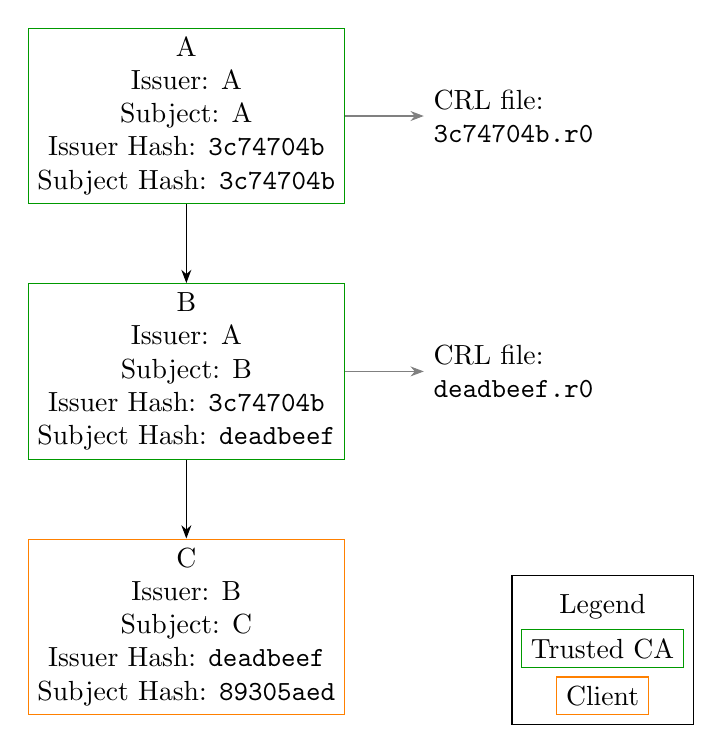
\begin{tikzpicture}
	% Styles.
	[ca/.style={rectangle,draw=green!60!black,minimum height=1cm,minimum width=1.5cm},
	leaf/.style={rectangle,draw=orange,minimum height=1cm, minimum width=1.5cm}]
	% Certificates.
	\node (A) at (0, 0) [ca,align=center] {A \\ Issuer: A \\ Subject: A \\ Issuer Hash: \texttt{3c74704b} \\ Subject Hash: \texttt{3c74704b}};
	\node (B) [below=of A] [ca,align=center] {B \\ Issuer: A \\ Subject: B \\ Issuer Hash: \texttt{3c74704b} \\ Subject Hash: \texttt{deadbeef}};
	\node (C) [below=of B] [leaf,align=center] {C \\ Issuer: B \\ Subject: C \\ Issuer Hash: \texttt{deadbeef} \\ Subject Hash: \texttt{89305aed}};
	\draw[-Stealth] (A) -- (B);
	\draw[-Stealth] (B) -- (C);
	\node (A CRL) [right=of A,align=left] {CRL file: \\ \texttt{3c74704b.r0}};
	\node (B CRL) [right=of B,align=left] {CRL file: \\ \texttt{deadbeef.r0}};
	\draw[-Stealth,gray] (A) -- (A CRL);
	\draw[-Stealth,gray] (B) -- (B CRL);
	% Legend.
	\node (lanchor) at (current bounding box.south east) {};
	\node (legend) at (lanchor) [above=1.1cm] {Legend};
	\node (l1) at (lanchor) [above=0.6cm,draw=green!60!black] {Trusted CA};
	\node (l2) at (lanchor) [above=0.0cm,draw=orange] {Client};
	\node [rectangle,draw,fit=(legend) (l1) (l2)] {};
\end{tikzpicture}
}
\end{makeimage}
\caption{Each CA requires its own CRL file.  The CRL file name is based on the hash of its issuer name.  Note that the \emph{issuer} of the CRL file is the \emph{subject} of its respective CA.}
\end{figure}
\end{center}

One more caveat: OpenSSL does not seem to report any error if the CRL path directory does not exist.  Figures.


% Syncing the Gentoo repository.
\section{2017-08-23 Securely Syncing the Gentoo Repository via a Local Server}

\begin{center}
\begin{figure}
\begin{makeimage}
\fbox{
\begin{tabular}{l|l}
Before: & After: \\
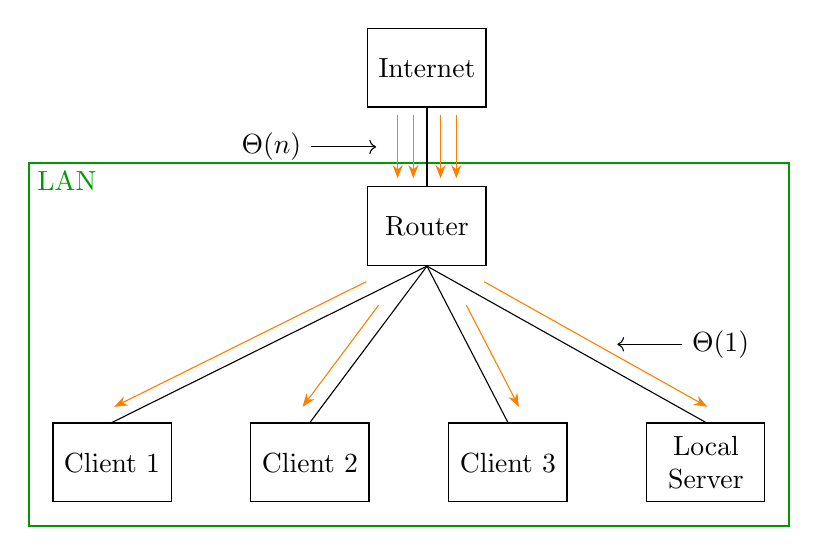
\begin{tikzpicture}
	% Machines.
	[puter/.style={rectangle,draw,minimum height=1cm,minimum width=1.5cm}]
	\node (client1)  at (0, 0) [puter] {Client 1};
	\node (client2)  [right=of client1] [puter] {Client 2};
	\node (client3)  [right=of client2] [puter] {Client 3};
	\node (server)   [right=of client3] [puter] {\parbox{1cm}{\centering Local \\ Server}};
	\node (router)   at (4, 3) [puter] {Router};
	\node (internet) [above=of router] [puter] {Internet};
	% Links.
	\draw (client1.north) -- (router.south)
		node[pos=0.1,left=0.2,circle](c1-r){}
		node[pos=0.9,left=0.2,circle](r-c1){};
	\draw (client2.north) -- (router.south)
		node[pos=0.1,left=0.07,circle](c2-r){}
		node[pos=0.75,left=0.07,circle](r-c2){};
	\draw (client3.north) -- (router.south)
		node[pos=0.1,right=0.07,circle](c3-r){}
		node[pos=0.75,right=0.07,circle](r-c3){};
	\draw (server.north) -- (router.south)
		node[pos=0.1,right=0.2,circle](s-r){}
		node[pos=0.9,right=0.2,circle](r-s){}
		node[pos=0.5,right=0.3,circle](smid){};
	\draw (router.north) -- (internet.south)
		node[pos=0.1,left=0.2,circle](r1-i1){}
		node[pos=0.1,left=0,circle](r2-i2){}
		node[pos=0.1,right=0,circle](r3-i3){}
		node[pos=0.1,right=0.2,circle](r4-i4){}
		node[pos=0.9,left=0.2,circle](i1-r1){}
		node[pos=0.9,left=0,circle](i2-r2){}
		node[pos=0.9,right=0,circle](i3-r3){}
		node[pos=0.9,right=0.2,circle](i4-r4){}
		node[pos=0.5,left=0.3,circle](mid){};
	% Traffic.
	\draw[orange,-Stealth] (r-c1.center) -- (c1-r.center);
	\draw[orange,-Stealth] (r-c2.center) -- (c2-r.center);
	\draw[orange,-Stealth] (r-c3.center) -- (c3-r.center);
	\draw[orange,-Stealth] (r-s.center) -- (s-r.center);
	\draw[orange,-Stealth] (i1-r1.center) -- (r1-i1.center);
	\draw[orange,-Stealth] (i2-r2.center) -- (r2-i2.center);
	\draw[orange,-Stealth] (i3-r3.center) -- (r3-i3.center);
	\draw[orange,-Stealth] (i4-r4.center) -- (r4-i4.center);
	\draw [<-] (mid) -- +(-1, 0) node[left]{$\Theta(n)$};
	\draw [<-] (smid) -- +(1, 0) node[right]{$\Theta(1)$};
	% LAN box.
	\begin{scope}[on background layer]
		\node (bback) [rectangle,thick,draw=green!60!black,inner sep=0.3cm,fit=(client1) (server) (router)] {};
		\node [below right,text=green!60!black] at (bback.north west) {LAN};
	\end{scope}
\end{tikzpicture}
&  % Copy+paste'd
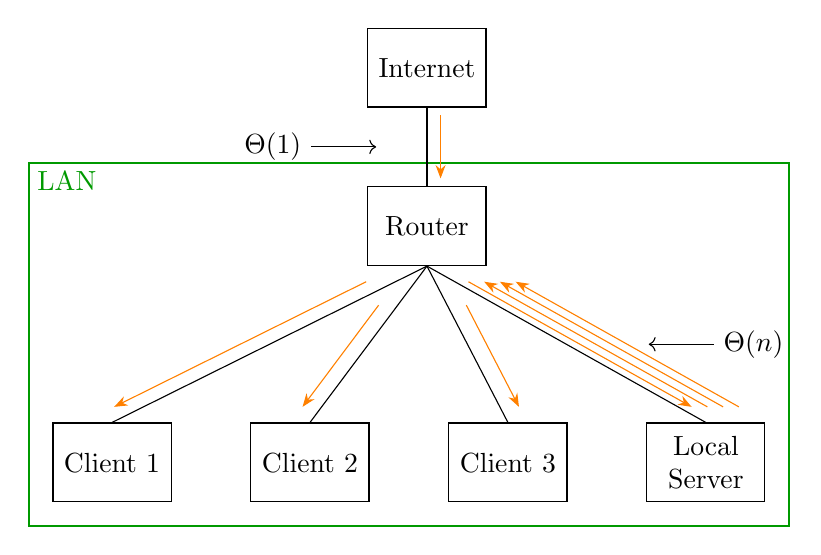
\begin{tikzpicture}
	% Machines.
	[puter/.style={rectangle,draw,minimum height=1cm,minimum width=1.5cm}]
	\node (client1)  at (0, 0) [puter] {Client 1};
	\node (client2)  [right=of client1] [puter] {Client 2};
	\node (client3)  [right=of client2] [puter] {Client 3};
	\node (server)   [right=of client3] [puter] {\parbox{1cm}{\centering Local \\ Server}};
	\node (router)   at (4, 3) [puter] {Router};
	\node (internet) [above=of router] [puter] {Internet};
	% Links.
	\draw (client1.north) -- (router.south)
		node[pos=0.1,left=0.2,circle](c1-r){}
		node[pos=0.9,left=0.2,circle](r-c1){};
	\draw (client2.north) -- (router.south)
		node[pos=0.1,left=0.07,circle](c2-r){}
		node[pos=0.75,left=0.07,circle](r-c2){};
	\draw (client3.north) -- (router.south)
		node[pos=0.1,right=0.07,circle](c3-r){}
		node[pos=0.75,right=0.07,circle](r-c3){};
	\draw (server.north) -- (router.south)
		node[pos=0.1,right=0,circle](s-r){}
		node[pos=0.9,right=0,circle](r-s){}

		node[pos=0.1,right=0.2,circle](s-c1){}
		node[pos=0.9,right=0.2,circle](c1-s){}
		node[pos=0.1,right=0.4,circle](s-c2){}
		node[pos=0.9,right=0.4,circle](c2-s){}
		node[pos=0.1,right=0.6,circle](s-c3){}
		node[pos=0.9,right=0.6,circle](c3-s){}

		node[pos=0.5,right=0.7,circle](smid){};
	\draw (router.north) -- (internet.south)
		node[pos=0.9,right=0,circle](i-s){}
		node[pos=0.1,right=0,circle](s-i){}
		node[pos=0.5,left=0.3,circle](mid){};
	% Traffic.
	\draw[orange,-Stealth] (r-c1.center) -- (c1-r.center);
	\draw[orange,-Stealth] (r-c2.center) -- (c2-r.center);
	\draw[orange,-Stealth] (r-c3.center) -- (c3-r.center);
	\draw[orange,-Stealth] (r-s.center) -- (s-r.center);
	\draw[orange,-Stealth] (s-c1.center) -- (c1-s.center);
	\draw[orange,-Stealth] (s-c2.center) -- (c2-s.center);
	\draw[orange,-Stealth] (s-c3.center) -- (c3-s.center);
	\draw[orange,-Stealth] (i-s.center) -- (s-i.center);
	\draw [<-] (mid) -- +(-1, 0) node[left]{$\Theta(1)$};
	\draw [<-] (smid) -- +(1, 0) node[right]{$\Theta(n)$};
	% LAN box.
	\begin{scope}[on background layer]
		\node (bback) [rectangle,thick,draw=green!60!black,inner sep=0.3cm,fit=(client1) (server) (router)] {};
		\node [below right,text=green!60!black] at (bback.north west) {LAN};
	\end{scope}
\end{tikzpicture}
\end{tabular}
}
\end{makeimage}
\caption{Using a local server for the Gentoo repository takes pressure off of the (often relatively slow) Internet connection and places it onto the (often relatively fast) LAN, especially important for those whose Internet is metered.}
\end{figure}
\end{center}

Running multiple Gentoo machines normally means keeping a copy of the Gentoo repository on each machine; by default this also means updating each copy of the repository by having each machine call out to the Gentoo mirrors on a regular basis for updates.  This is a waste of both local and upstream bandwidth and resources, because, within a given time period, the repository is the exact same regardless of the type of machine it is on; instead, it is more efficient to set up one machine as a server that synchronizes with upstream, then have the other local machines synchronize to said local server.  This guide will explain how to do that securely.

Though there are multiple protocols that Portage can use for synchronization, this guide will cover only SSH, and \texttt{rsync+stunnel}.  Both of these are secure, allowing synchronization over an untrusted network, albeit the local server must be trusted.  Securely syncing the server to the upstream repository with \texttt{FEATURES=webrsync-gpg} is not covered here, as it is instead covered \htmladdnormallink{here}{https://wiki.gentoo.org/wiki/Handbook:AMD64/Working/Features#Validated_Gentoo_repository_snapshots}.

\subsection{SSH Synchronization}
One of the pros of SSH-based synchronization is that it requires no extra server configuration for machines that already have SSH access to the server.  The downside is that SSH access means shell access, which might not be desirable if any of the local machines is not fully trusted, for example, because it is running proprietary applications for, say, video games; one could try and circumvent this potential security weakness by giving the SSH user a restricted shell such as \texttt{rssh}, but I was unable to get \texttt{rssh} working with the \texttt{rsync} arguments that Portage wanted to use (note: Portage calls \texttt{rsync} over the SSH session).  Thus I prefer \texttt{rsync+stunnel}, but am including the SSH method for completeness and possible future reference.
\subsubsection{Server} Assuming that \texttt{sshd} is already set up (find one of many guides if it is not), the only thing that may need to be done is to add a special user for synchronization.  In order to add the user, run
\begin{quote}
\begin{verbatim}
	# useradd -m -s /bin/bash rsyncuser
	# passwd rsyncuser
\end{verbatim}
\end{quote}
\ldots then edit the SSH daemon configuration file, usually \texttt{/etc/ssh/sshd_config}, to contain the following line:
\begin{quote}
\begin{verbatim}
	AllowUsers rsyncuser
\end{verbatim}
\end{quote}
Depending on the selected authentication method for SSH, this may be enough to give the user access; however, in the case that only key-based authentication is allowed (usually via something like \texttt{PasswordAuthentication no} \& \texttt{ChallengeResponseAuthentication no} in \texttt{sshd_config}) an SSH keypair will need to be generated for the user and the private key copied to each client that wishes to synchronize with the server.  This can be done with the following commands:
\begin{quote}
\begin{verbatim}
	# cd /home/rsyncuser
	# su rsyncuser
	$ umask 0066
	$ mkdir -p .ssh
	$ ssh-keygen -a 16 -t ed25519
	$ cp .ssh/id_ed25519.pub .ssh/authorized_keys
\end{verbatim}
\end{quote}
This will create a keypair for the \texttt{rsyncyser} and authorize that keypair for SSH login.  The \texttt{.ssh/id_ed25519} file (the private key) will then need to be copied to the client machines, probably via a USB storage device:
\begin{quote}
\begin{verbatim}
	# cp .ssh/id_ed25519 /path/to/probably/usb/storage/device
\end{verbatim}
\end{quote}

This ends the server-side configuration.

\subsubsection{Clients}
By default, Portage knows how to use SSH for synchronization, so basic setup is quite simple, although some of the details are rather esoteric.

In order to tell Portage to synchronize over SSH, if it hasn't been done already, set up the main repository configuration via:
\begin{quote}
\begin{verbatim}
	# mkdir -p /etc/portage/repos.conf
	# cp /usr/share/portage/config/repos.conf /etc/portage/repos.conf/gentoo.conf
\end{verbatim}
\end{quote}
This creates, at the time of this writing, at least, a sane configuration file for the default repository that can then be reconfigured.  With this file created, Portage should function as it always has; the defaults must be overridden in order to actually change its behavior. In order to use SSH, edit the \texttt{/etc/portage/repos.conf/gentoo.conf} file by changing the \texttt{sync-uri} option under the \texttt{[gentoo]} section to read:
\begin{quote}
\begin{verbatim}
	sync-uri = ssh://rsyncuser@192.168.1.1/usr/portage
\end{verbatim}
\end{quote}
\ldots where \texttt{192.168.1.1} is replaced with the network address of the local server.  Portage will now begin trying to sync via SSH.

"Trying" may be the modus operandi depending on whether or not the local server strictly requires keys or will accept user passwords; it is thus useful to understand where Portage stores its SSH information, as its home directory is not \texttt{/home/portage}, but, as \texttt{/etc/passwd} reveals, \texttt{/var/tmp/portage}, thus SSH configuration goes into \texttt{/var/tmp/portage/.ssh}.  In order to get Portage to use \texttt{rsyncuser}'s key, run the following:
\begin{quote}
\begin{verbatim}
	# mkdir -p /var/tmp/portage/.ssh
	# umask 0066
	# cp /path/from/probably/usb/device/with/rsyncusers/key/id_ed25519 /var/tmp/portage/.ssh/id_ed25519
	# chown -R portage:portage /var/tmp/portage/.ssh
\end{verbatim}
\end{quote}
Portage should now pickup \texttt{rsyncuser}'s key when it tries to synchronize.

Admittedly, storing valuable authentication information in a \texttt{/var/tmp} subdirectory seems risky at best.  Another option for storing the key is to place the key at a more stable location and then tell Portage where to find it.  Start by placing the key somewhere safer:
\begin{quote}
\begin{verbatim}
	# mkdir -p /usr/local/portage/.ssh
	# chmod 700 /usr/local/portage/.ssh
	# chown -R portage:portage /usr/local/portage/.ssh
	# mv /var/tmp/portage/.ssh/id_ed25519 /usr/local/portage/.ssh/
\end{verbatim}
\end{quote}
\ldots then tell Portage where to find the key by adding the following line to \texttt{/etc/portage/make.conf}:
\begin{quote}
\begin{verbatim}
	PORTAGE_SSH_OPTS="-i /usr/local/portage/.ssh/id_ed25519"
\end{verbatim}
\end{quote}
Portage will now look for the \texttt{rsyncuser}'s key at the previously-specified location.

This solves the \texttt{rsyncuser}'s key problem, but what about the important \texttt{known_hosts} file?  Well, I didn't get that far.  I don't fully trust of all my machines, and do not want to give all of them shell access to my server, and, since I couldn't get \texttt{rssh} to work with Portage and was looking for an excuse to play with \texttt{stunnel}, I decided to work on it instead, thus \texttt{rsync+stunnel} is the topic of the next section.

\subsection{Rsync+stunnel Synchronization}
This method works by using an \texttt{rsync} daemon to synchronize between the local server and client; however, because \texttt{rsync} is unencrypted, the connection is wrapped via the \texttt{stunnel} daemon, which uses \htmladdnormallink{TLS}{https://en.wikipedia.org/wiki/Transport_Layer_Security} for encryption and authentication.  \texttt{stunnel} must be configured on both the local server and each client.

\subsubsection{Server}
Start by setting up the \texttt{rsync} daemon without \texttt{stunnel}.  By default, Gentoo comes with a disabled but sane configuration file at \texttt{/etc/rsyncd.conf}.  Adding a few extra lines gives, excluding comments, the following:
\begin{quote}
\begin{verbatim}
	pid file = /run/rsyncd.pid
	use chroot = yes
	read only = yes
	hosts allow = 192.168.1.1/16
	reverse lookup = no
	timeout = 60

	[gentoo-portage]
	path = /usr/portage
	comment = Gentoo Portage tree
	exclude = /distfiles /packages
\end{verbatim}
\end{quote}
By default this configuration file creates an \texttt{rsync} \textit{module} that clients can synchronize with; this module is read-only and excludes directories that are not a part of the repository.  The extra options are: \texttt{hosts allow = 192.168.1.1/16}, which tells \texttt{rsync} to only accept connections from hosts in the specified block and must be appropriate to the local network; \texttt{reverse lookup = no}, which disables reverse-DNS lookups of client IP addresses; and \texttt{timeout = 60}, which sets a small timeout for unresponsive clients.  See \texttt{man 5 rsyncd.conf} for details; the extra options are not strictly necessary for the purposes of this guide.

The next step is to install and configure \texttt{stunnel}.  This involves four steps: installing the program, configuring the service, generating certificates, and creating the service: To install \texttt{stunnel}, run:
\begin{quote}
\begin{verbatim}
	# emerge -av stunnel
\end{verbatim}
\end{quote}
For convenience, the Gentoo developers created a useful example configuration file for \texttt{rsync+stunnel} which may be installed by running:
\begin{quote}
\begin{verbatim}
	USE="stunnel" emerge -av rsync
\end{verbatim}
\end{quote}
This creates the file \texttt{/etc/stunnel/rsyncd.conf}.  Move it to \texttt{/etc/stunnel/rsyncd-stunnel.conf} for \texttt{init} scripts (later), and reconfigure it such that, excluding comments, it has the following options:
\begin{quote}
\begin{verbatim}
	foreground = no
	pid = /var/run/stunnel/rsyncd-stunnel.pid
	socket = l:TCP_NODELAY=1
	socket = r:TCP_NODELAY=1
	setuid = root
	setgid = root

	[rsync]
	accept = 874
	cert = /etc/stunnel/rsyncd-stunnel.crt
	key  = /etc/stunnel/rsyncd-stunnel.key
	client = no

	exec = /usr/bin/rsync
	execargs = rsync --server --daemon --config=/etc/rsyncd.conf .
\end{verbatim}
\end{quote}
Most of these options come with the default configuration file, but make sure to change the \texttt{pid} option.  The \texttt{cert} and \texttt{key} options specify where the \htmladdnormallink{X.509}{https://en.wikipedia.org/wiki/X.509} certificate and its key are to be loaded from (they will be generated later).  Port \texttt{874} is used in place of \texttt{873}, as it is not a plaintext \texttt{rsync} service.  Client verification is not wanted here, so make sure to remove any \texttt{verify} and \texttt{CAfile} lines.

In order to generate the server's certificate, run the following series of commands:
\begin{quote}
\begin{verbatim}
	# cd /etc/stunnel
	# umask 0077
	# openssl genrsa -out rsyncd-stunnel.key 4096
	# openssl req -key rsyncd-stunnel.key -new -x509 -days 7200 -sha512 -out rsyncd-stunnel.crt -subj '/CN=rsyncd-stunnel/'
\end{verbatim}
\end{quote}
The short story here is that this will create a certificate and key pair for TLS that will last for almost 20 years, see \texttt{man genrsa} and \texttt{man req} for details.

Finally, create the service with:
\begin{quote}
\begin{verbatim}
	# cd /etc/init.d
	# ln -s stunnel rsyncd-stunnel
\end{verbatim}
\end{quote}
This uses the default \texttt{stunnel} init script, except it will look for a configuration file at \texttt{/etc/stunnel/rsyncd-stunnel.conf}, hence the earlier renaming that was done.  To start the service, run \texttt{rc-service rsyncd-stunnel start}, and don't forget to add it to the default runlevel via:
\begin{quote}
\begin{verbatim}
	# rc-update add rsyncd-stunnel default
\end{verbatim}
\end{quote}

The server should now be configured and ready for synchronization.  The clients must now be configured to trust and use the server.

\subsubsection{Clients}
The client must now be configured so that when Portage attempts to sync it will use the secure connection \textbf{and} it will validate that it is syncing with the server, otherwise a malicious actor could imitate the server and send a compromised repository.  This involves installing and configuring \texttt{stunnel}, configuring Portage, then creating the service.

Begin by installing \texttt{stunnel}:
\begin{quote}
\begin{verbatim}
	# emerge -av stunnel
\end{verbatim}
\end{quote}
\ldots then configure \texttt{stunnel} so that, without comments, the configuration file \texttt{/etc/stunnel/stunnel.conf} reads:
\begin{quote}
\begin{verbatim}
	setuid = stunnel
	setgid = stunnel
	pid = /run/stunnel/stunnel.pid
	socket = l:TCP_NODELAY=1
	socket = r:TCP_NODELAY=1

	[rsync-stunnel]
	client     = yes
	CAfile     = /etc/stunnel/rsyncd-stunnel.crt
	verifyPeer = yes
	accept     = 127.0.0.1:873
	connect    = 192.168.1.200:874
\end{verbatim}
\end{quote}
This creates an \texttt{stunnel} \emph{service}.  The \texttt{client} argument lets \texttt{stunnel} know to run \texttt{rsync} as a client rather than as a server.  The \texttt{CAfile} argument specifies the location of the server certificate to use (note that it has not yet been copied over to the client).  The \texttt{verifyPeer} is especially important as enabling it will actually validate the server certificate; without this enabled a malicious actor could intercept and modify the traffic.  The \texttt{accept} argument specifies where the \texttt{stunnel} program will listen for client connections, Portage will later be configured to make connections here.  The \texttt{connect} argument specifies where the \texttt{stunnel} program will connect to; it must be set to the address and port of the local server.  The other options are fairly standard.  Note that, unlike the server, this setup is using the default \texttt{stunnel} settings, configuring multiple \texttt{stunnel} services at the OpenRC level would require modifying a few parameters, such as the PID (Process ID) and the filename of the configuration.

Now that \texttt{stunnel} has been configured, make sure to copy the certificate from the local server to the client.  This should be done via a trusted storage device (USB stick, SD Card, \&c.) or the certificate retrieved via a command such as OpenSSL's \texttt{s\_client} (usage not covered here) and its fingerprint manually verified.
\begin{quote}
\begin{verbatim}
	# cp /path/from/secure/storage/device /etc/stunnel/rsyncd-stunnel.crt
\end{verbatim}
\end{quote}
\texttt{stunnel} now has all that it needs to securely tunnel a connection to the server.

Portage must now be configured to use the secure tunnel.  As with SSH configuration, begin by overriding the default repository configuration:
\begin{quote}
\begin{verbatim}
	# mkdir -p /etc/portage/repos.conf
	# cp /usr/share/portage/config/repos.conf /etc/portage/repos.conf/gentoo.conf
\end{verbatim}
\end{quote}
\ldots then modify the \texttt{sync-uri} argument to correspond to the \texttt{accept} argument configured in \texttt{stunnel}:
\begin{quote}
\begin{verbatim}
	sync-uri = rsync://127.0.0.1:873/gentoo-portage
\end{verbatim}
\end{quote}
This will synchronize with the \texttt{gentoo-portage} module defined on the local server's \texttt{/etc/rsyncd.conf}.  Note how the use of \texttt{stunnel} is completely transparent to Portage.  This has the minor disadvantage that error diagnostics must be found in log message from \texttt{stunnel} and not the Portage frontend, but is usually not a problem once things have been configured properly.

Next, start the service and add it to the default runlevel:
\begin{quote}
\begin{verbatim}
	# rc-service stunnel start
	# rc-update add stunnel default
\end{verbatim}
\end{quote}
\ldots then try it out with:
\begin{quote}
\begin{verbatim}
	# emerge --sync
\end{verbatim}
\end{quote}
Portage should now be securely synchronizing to the local server!  Repeat these steps for each client that needs to synchronize with the local server.


% Ancient Apparition Bowling
\section{2017-07-17 Ancient Apparition Bowling}
This is a silly metagame that I came up with for a DotA2 custom game.  It may not be possible to beat, but I've yet to try all strategies.

\subsection*{Origin}
Mercilessly slaughtering bots using weird combinations of cheats in DotA2 is an easy way to blow off a little steam after a difficult match.  One day I decided to go "bowling" with Ancient Apparition; I'd cheat to maximum level, 6-slot, enable wtf mode, and snipe the bots from base with his ultimate.
This is loads of fun, until the creeps start pushing towers, at which point the bots also take advantage of wtf mode and begin spamming fortify, leading to a frustrating stalemate.  The workaround for this is to disable wtfmode and instead use the \texttt{-refresh} cheat, which, although it does reset fortify cooldowns, can be used in conjunction with a Refresher Orb to blast the bots with two ultimates while giving them only one fortify.

The result is a semi-functional slaughtering of bots, although having to constantly open the command prompt to paste and submit the \texttt{-refresh} command gets annoying after a while; sadly, there doesn't seem to be a way to disable the bots' fortify spam.  After a little bit of this, I noticed that the cooldown of the metaphorical bowling ball and the travel time were not that far apart, leading me to wonder if I could play this game successfully without having to spam cheat commands (and reset the fortify cooldown) all game long.  Thus "Ancient Apparition Bowling" was born.

\subsection*{Rules}
These are the rules of the game, and though they may not be comprehensive, you should be able to understand the jist of them.  First, stay in fountain for the duration of the match.  Second, use cheats to give yourself max level (\texttt{-lvlup 25}), 6-slots (\texttt{-item <name>}), and vision (\texttt{-allvision}).  Third, no backpack, stash, or other item-use shenanegains; stick to your 6 slots.  Fourth, no bots on your team and five bots of highest difficulty on the other team.  That's it!
\begin{figure}
\includegraphics[scale=0.33]{files/blog/2017_07_17_ancient_apparition_bowling/fountain.png}
\caption{Where you will be spending all of your time.}
\end{figure}

Your goal is now to destroy the bots' ancient before the bots level up enough to tank through your ult and push your base.  This is more difficult than it sounds, as the bots are actually rather crafty and level up sooner than you might expect.

\subsection*{Strategy}
My current build involves getting an Aghaim's Scepter, Octarine Core, Refresher Orb, and 3 Aether Lens.  Perhaps you can think up something better.
\begin{figure}
\includegraphics{files/blog/2017_07_17_ancient_apparition_bowling/items.png}
\end{figure}

It is difficult to push all lanes at once, since the bots can quickly respawn at lower levels, and you only have so many ultimates to shoot off.  It would thus seem prudent to choose a particular lane to hammer, but how to do so isn't actually obvious.

The strategy that I tried was to focus the enemy creeps at their spawning point in a side lane.  This can be done by firing consistently at the 18 and 48 second marks towards the front of their 3rd tower. This will obliterate all of the creeps during the early part of the game.  Make sure to adjust your ultimate slightly to the left each time in order to adjust for the micro-delay between your ult going off cooldown and actually launching your ult; you can reset this after a while with a Refresher Orb.
\begin{figure}
\includegraphics[scale=0.33]{files/blog/2017_07_17_ancient_apparition_bowling/towerhit.png}
\caption{Killing creeps as soon as they spawn.}
\end{figure}

Though this may at first seem like a good way to get the creeps to push the tower, the bots are actually crafty enough to pull the creeps behind the tower, limiting the amount of damage done.  While I was able to eventually push to their barracks, at this point the other bots also helped pull the creeps behind the barracks, and eventually became strong enough to tank the ult and push my base, thus making this a losing strategy.
\begin{figure}
\includegraphics[scale=0.33]{files/blog/2017_07_17_ancient_apparition_bowling/botpull.png}
\caption{Sneaky bots pulling creeps away from the tower.}
\end{figure}

A possible variation would be to try focusing down the bots themselves, but this is tricky as they often move out of the ult's way.  A hybrid combination may involve finding a position where the bots and creeps are likely to align, then aiming to kill the creeps and probably the bots.  It may also be easier to push straight up middle rather than taking out a side lane first, especially as the bots seem found of charging up mid.

I've yet to win at this metagame.  It might not even be plausible.  Try it yourself and see what happens!

\subsection*{Addendum}
Between inventing this game, writing this article, and getting the screenshots, the bot fortify spam in wtf mode seems to have stopped.

\end{document}
